\documentclass[11pt,oneside]{book}
\usepackage{fontspec}
\setmainfont{Noto Serif}
\setsansfont{Noto Sans}
\setmonofont{Noto Sans Mono}
\newfontfamily\proseunicodefont{DejaVu Serif}
\usepackage[margin=1in]{geometry}
\usepackage{microtype}
\usepackage{amsmath,amssymb,amsthm,mathtools,bm}
\usepackage{graphicx}
\usepackage{xcolor}
\usepackage{booktabs}
\usepackage{array}
\usepackage{longtable}
\usepackage{enumitem}
\usepackage{float}
\usepackage{caption}
\usepackage{hyperref}
\usepackage{fancyhdr}
\usepackage{tikz}
\usetikzlibrary{arrows.meta,positioning,calc,decorations.pathmorphing}

\hypersetup{
  colorlinks=true,
  linkcolor=blue!50!black,
  urlcolor=blue!50!black,
  citecolor=blue!50!black
}

\setlength{\parskip}{0.5em}
\setlength{\parindent}{0pt}
\setlist[itemize]{topsep=0.25em,itemsep=0.2em}
\setlist[enumerate]{topsep=0.25em,itemsep=0.2em}
\setlength{\headheight}{40pt}
\numberwithin{equation}{chapter}

\newtheorem{theorem}{Теорема}[chapter]
\newtheorem{proposition}[theorem]{Утверждение}
\newtheorem{lemma}[theorem]{Лемма}
\newtheorem{corollary}[theorem]{Следствие}
\theoremstyle{definition}
\newtheorem{definition}[theorem]{Определение}
\newtheorem{example}[theorem]{Пример}
\theoremstyle{remark}
\newtheorem{remark}[theorem]{Замечание}

\providecommand{\ket}[1]{\left\lvert#1\right\rangle}
\providecommand{\bra}[1]{\left\langle#1\right\rvert}
\providecommand{\braket}[2]{\left\langle#1\,\middle|\,#2\right\rangle}
\providecommand{\expect}[1]{\left\langle#1\right\rangle}
\newcommand{\lectureoverview}[1]{\paragraph{Обзор.} #1}
\newenvironment{classroomqa}{%
  \par\medskip
  \begin{quote}\small
}{%
  \end{quote}
  \medskip
}
\newcommand{\audiencequestion}[1]{\noindent\textbf{Вопрос из аудитории.} #1\par\smallskip}
\newcommand{\classquestion}[1]{\noindent\textbf{Вопрос аудитории.} #1\par\smallskip}
\newcommand{\lecturerresponse}[1]{\noindent\textbf{Ответ.} #1\par}
\newcommand{\lecturetimestamp}[1]{\footnote{Время в лекции: #1.}}
\newcommand{\lectureframe}[1]{\par\smallskip{\centering\footnotesize\itshape Кадр лекции: #1.\par}}

\makeatletter
\newcommand{\course@headerfont}{\normalfont\small\itshape}
\newcommand{\course@pagefont}{\normalfont\small}
\newcommand{\course@headerraise}{14pt}
\newlength{\course@headerboxheight}
\setlength{\course@headerboxheight}{\dimexpr\headheight-\course@headerraise-9pt\relax}
\newcommand{\course@leftheadbox}[1]{%
  \raisebox{\course@headerraise}{%
    \parbox[t][\course@headerboxheight][t]{0.82\textwidth}{%
      \raggedright\course@headerfont\strut\MakeUppercase{#1}\strut%
    }%
  }%
}
\newcommand{\course@rightheadbox}[1]{%
  \raisebox{\course@headerraise}{%
    \parbox[t][\course@headerboxheight][t]{0.82\textwidth}{%
      \raggedleft\course@headerfont\strut\MakeUppercase{#1}\strut%
    }%
  }%
}
\renewcommand{\chaptermark}[1]{\markboth{\MakeUppercase{\chaptername\ \thechapter.\ #1}}{}}
\renewcommand{\sectionmark}[1]{\markright{\MakeUppercase{\thesection\hspace{0.4em}#1}}}
\fancyhf{}
\fancyhead[L]{\course@leftheadbox{\leftmark}}
\fancyhead[R]{\course@pagefont\thepage}
\renewcommand{\headrulewidth}{0.5pt}
\pagestyle{fancy}
\fancypagestyle{plain}{%
  \fancyhf{}
  \fancyhead[L]{\course@leftheadbox{\leftmark}}
  \fancyhead[R]{\course@pagefont\thepage}
  \renewcommand{\headrulewidth}{0.5pt}
}
\makeatother

\usepackage{polyglossia}
\setdefaultlanguage{russian}
\usepackage{sectsty}
\renewcommand{\contentsname}{Содержание}
\renewcommand{\chaptername}{Глава}
\renewcommand{\figurename}{Рисунок}
\renewcommand{\tablename}{Таблица}
\renewcommand{\proofname}{Доказательство}
\renewcommand{\bibname}{Литература}
\sectionfont{\raggedright}
\subsectionfont{\raggedright}
\makeatletter
\renewcommand{\@pnumwidth}{2.2em}
\renewcommand{\@tocrmarg}{3.2em}
\makeatother
\usepackage{tocloft}
\renewcommand{\cftchapfont}{\small\bfseries}
\renewcommand{\cftchappagefont}{\small\bfseries}
\renewcommand{\cftsecfont}{\small}
\renewcommand{\cftsecpagefont}{\small}
\setlength{\cftsecnumwidth}{3em}
\renewcommand{\cftsubsecfont}{\small}
\renewcommand{\cftsubsecpagefont}{\small}
\setlength{\cftsubsecindent}{4.5em}
\setlength{\cftsubsecnumwidth}{4em}
\emergencystretch=6em
\pdfstringdefDisableCommands{\def\proseunicodefont{}}

\geometry{paperwidth=177.6mm,paperheight=252mm,left=16mm,right=16mm,
 top=18mm,bottom=18mm,includeheadfoot,headheight=28pt,headsep=7mm,footskip=9mm}
\usepackage{scrextend}
\changefontsizes[17pt]{12pt}
\raggedbottom
\renewenvironment{classroomqa}{\par\medskip\begingroup}{\par\endgroup\medskip}
\fancyhf{}
\setlength{\headwidth}{\textwidth}
\fancyhead[L]{\parbox{\textwidth}{\raggedright\fontsize{9}{11}\selectfont\nouppercase{\leftmark}}}
\fancyfoot[C]{\small\thepage}
\renewcommand{\headrulewidth}{0.3pt}
\fancypagestyle{plain}{\fancyhf{}\fancyfoot[C]{\small\thepage}\renewcommand{\headrulewidth}{0pt}}

\graphicspath{{../../../generated_course_notes/core/statistical_mechanics/2013_spring_theoretical_minimum/figures/}{../../../generated_course_notes/core/statistical_mechanics/2013_spring_theoretical_minimum/assets/}}
\hypersetup{
  pdftitle={Statistical Mechanics: The Theoretical Minimum},
  pdfauthor={Leonard Susskind; companion notes edited by LazyingArt LLC with Video2Book},
  pdfsubject={Core track, 2013 Spring},
  pdfkeywords={Leonard Susskind, statistical mechanics, thermodynamics, Ising model, critical phenomena}
}
\begin{document}
\frontmatter
\hypersetup{pageanchor=false}
\begin{titlepage}
\hyphenpenalty=10000\exhyphenpenalty=10000
\thispagestyle{empty}
\begin{tikzpicture}[remember picture,overlay]
  \node[anchor=south west,inner sep=0] at (current page.south west) {%
    \includegraphics[width=\paperwidth,height=\paperheight,keepaspectratio=false]{../../../generated_course_notes/core/statistical_mechanics/2013_spring_theoretical_minimum/assets/cover-art.png}%
  };
  \node[
    anchor=north west,
    align=left,
    text width=0.78\paperwidth,
    fill=white,
    fill opacity=0.9,
    rounded corners=8pt,
    inner xsep=10pt,
    inner ysep=8pt
  ] at ([xshift=0.08\paperwidth,yshift=-0.06\paperheight]current page.north west) {%
    {\fontsize{30}{33}\selectfont\bfseries\color{black!88} Статистическая механика\\[0.85em]}
    {\large\color{black!72} Русское издание / весна 2013, теоретический минимум}
  };
  \node[
    anchor=south west,
    align=left,
    text width=0.68\paperwidth,
    fill=white,
    fill opacity=0.82,
    text opacity=1,
    rounded corners=6pt,
    inner sep=12pt
  ] at ([xshift=0.08\paperwidth,yshift=0.08\paperheight]current page.south west) {%
    {\normalsize\color{black!78} Оригинальные лекции: Leonard Susskind\\[0.35em]}
    {\small\color{black!72} Сопроводительное издание: \href{https://lazying.art}{LazyingArt LLC} / \href{https://github.com/lachlanchen/Video2Book}{Video2Book}.}
  };
\end{tikzpicture}
\mbox{}
\end{titlepage}
\hypersetup{pageanchor=true}

\chapter*{Об этих конспектах}
Эти самостоятельно отредактированные сопроводительные конспекты следуют лекциям Леонарда Сасскинда 2013 года по статистической механике. Они сохраняют принятый в лекциях порядок изложения, содержательные обсуждения в аудитории, математические выводы и избранные записи с доски. Они не являются оригинальной рукописью профессора Сасскинда и не были им проверены или одобрены.

Это издание подготовлено \href{https://lazying.art}{LazyingArt LLC} с использованием рабочего процесса \href{https://github.com/lachlanchen/Video2Book}{Video2Book} с открытым исходным кодом. Полные машинные расшифровки и файлы субтитров по-прежнему доступны отдельно в репозитории и могут содержать ошибки распознавания.
\clearpage
\tableofcontents
\mainmatter
\chapter{Вероятность, информация и энтропия}

\lectureoverview{Статистическая механика начинается там, где микроскопический закон встречается с неполным знанием. Сначала мы придадим вероятности точный смысл, затем спросим, как само детерминированное движение задаёт вероятности, как законы сохранения разбивают пространство состояний и почему динамика, сохраняющая информацию, естественным образом приводит к энтропии. Первый и нулевой законы вступают в игру лишь после того, как эта структура установлена.}

\section{Зачем нужна статистическая механика?}

Статистическую механику иногда описывают как старую физику. Такое описание упускает главное. Она и досовременна, и современна и, вероятно, останется полезной в любой постсовременной физике, которая придёт на смену известным нам теориям. Частные модели возникают и исчезают; второй закон термодинамики снова и снова сохранялся как ориентир. Всякий раз, когда предлагаемое описание природы как будто создаёт порядок даром, принципиально уничтожает информацию или сводит замкнутую систему к неестественно простому состоянию, второй закон предупреждает нас, что что-то было упущено.

Эта дисциплина может казаться менее эффектной, чем вновь открытая частица, но она по меньшей мере столь же глубока и гораздо более обща. Газы, жидкости, твёрдые тела, излучение, чёрные дыры, информация и квантовые поля — всё это требует статистических рассуждений. Более того, без неё нельзя было бы понять экспериментальный аппарат, использованный для открытия частиц. Вот почему поколения сильных физиков овладевали статистической механикой, даже когда их основная работа лежала в других областях: эта дисциплина полезна, но, кроме того, необычайно красива.

Чтобы понять, зачем она нужна, начнём с идеала, задаваемого механикой. Замкнутая система — это либо вся рассматриваемая вселенная, либо подсистема, достаточно хорошо изолированная, чтобы окружение на неё не влияло. Если нам известны её начальное состояние и закон эволюции, то классическая механика даёт полное предсказание. Квантовая механика изменяет то, что может быть предсказано, но и в ней есть точно определённое состояние и закон, предсказывающий максимум информации, допускаемый теорией.

Между предсказанием в принципе и полезным пониманием существует резкое различие. Список положений и скоростей всех молекул в этой комнате был бы невероятно длинным, почти сразу изменился бы и ответил бы лишь на немногие из вопросов, которые нас действительно интересуют. Поэтому точные микроскопические законы могут одновременно обладать полной предсказательной силой и быть практически бесполезными.

Статистическая механика — это теория вероятностей, применённая к данной физической ситуации. Она становится необходимой, когда начальное состояние известно не с совершенной точностью, когда закон известен лишь приближённо, когда система открыта или просто когда число микроскопических переменных слишком велико, чтобы их отслеживать. Ничто из этого не означает слабости предсказаний. Большие числа часто делают статистические предсказания чрезвычайно точными.

Рассмотрим изолированный ящик с газом. Мы не можем предсказать траекторию каждой молекулы, однако немногие макроскопические данные позволяют нам с высокой точностью предсказывать давление, энергию и многие другие макроскопические величины. Неопределёнными остаются флуктуации. В непредсказуемый момент малая область может содержать больше молекул, чем в среднем, тогда как другая содержит меньше. Такое событие лежит в хвосте распределения вероятностей: оно маловероятно, но не запрещено. Мы можем вычислить, как часто должны происходить такие флуктуации, не предсказывая момент конкретного появления одной из них.

Подбрасывание монеты демонстрирует то же различие. В миллиарде честных бросков числа орлов и решек будут близки друг к другу. Длинная серия орлов в конце концов возникнет, если бросать достаточно долго, но теория вероятностей предсказывает её частоту, а не указывает заранее, когда именно это произойдёт. Статистическая механика предназначена для систем, элементы которых слишком малы, слишком многочисленны или и то и другое одновременно.

В этом курсе будут развиты законы, а также их приложения к веществу. Эта дисциплина вознаграждает многократное изучение: её изучают, забывают часть материала, а затем изучают снова, уже глубже понимая, какие идеи являются фундаментальными. Мы начнём с идеи, которая определяет всё дальнейшее.

\section{Вероятность как исходный язык}

Почему вероятность работает, не объясняется самим исчислением вероятностей. Вероятностное предсказание может не оправдаться в отдельном испытании; именно это и означает, что исход возможен, но маловероятен. Теория говорит нам, как распределены исключения. Она не устраняет их. Поэтому мы принимаем вероятность как исходное понятие и формулируем правила, которым она подчиняется.

\subsection{Состояния и нормировка}

Пусть \(i\) обозначает возможный исход или возможное состояние системы. Для одной монеты \(i\) может означать орёл или решку. Для одного игрального кубика этот индекс может принимать значения от \(1\) до \(6\). Для двух кубиков пара индексов задаёт оба выпавших значения. Мы начнём с конечного дискретного пространства состояний,
\begin{equation}
 i=1,\ldots,N,
\end{equation}
а позже перейдём к бесконечному числу состояний и к непрерывному множеству состояний.

Незнание не означает, что у системы нет состояния. Оно означает, что мы не знаем, какое именно состояние она имеет, поэтому каждой возможности мы приписываем вероятность \(p_i\). Основные правила таковы:
\begin{align}
 p_i &\geq 0, \label{eq:sm1-prob-positive}\\
 \sum_{i=1}^{N}p_i &=1. \label{eq:sm1-prob-normalization}
\end{align}
Альтернативы взаимно исключают друг друга и исчерпывают все возможности: реализуется ровно одна из них. Отрицательным вероятностям здесь места нет, а сумма равна единице, потому что должен реализоваться некоторый допустимый исход.

\subsection{Частота и закон больших чисел}

Вероятность связывается с экспериментом посредством повторных испытаний. Предположим, что один и тот же эксперимент проводится \(N_{\mathrm{trials}}\) раз, и пусть \(N(i)\) — число испытаний, в которых получается исход \(i\). Тогда частотная интерпретация имеет вид
\begin{equation}
 p_i=
 \lim_{N_{\mathrm{trials}}\to\infty}
 \frac{N(i)}{N_{\mathrm{trials}}}.
 \label{eq:sm1-frequency}
\end{equation}
Это физическая гипотеза, выраженная через идеальный предел. Ни одна лаборатория не проводит бесконечно много экспериментов. Утверждение состоит в том, что при достаточно большом числе испытаний отношение становится достаточно близким к \(p_i\) для нужного предсказания. Конечные выборки флуктуируют вокруг предельного значения.

\subsection{Средние значения}

Теперь сопоставим каждому состоянию число \(f(i)\). Это может быть энергия, импульс или любая другая величина, которую мы хотим измерить. Математическое ожидание этой величины равно
\begin{equation}
 \langle f\rangle=\sum_i f(i)p_i.
 \label{eq:sm1-expectation}
\end{equation}
Обозначение угловыми скобками удобно и вне квантовой механики. На языке частот то же среднее имеет вид
\begin{equation}
 \langle f\rangle
 =
 \lim_{N_{\mathrm{trials}}\to\infty}
 \frac{1}{N_{\mathrm{trials}}}
 \sum_i f(i)N(i).
 \label{eq:sm1-frequency-average}
\end{equation}

Для монеты определим
\begin{equation}
 f(\mathrm{H})=+1,
 \qquad
 f(\mathrm{T})=-1.
\end{equation}
Если орёл и решка имеют вероятности \(1/2\) каждая, то
\begin{equation}
 \langle f\rangle
 =(+1)\frac12+(-1)\frac12=0.
\end{equation}
Среднее не обязано быть возможным исходом. Монета никогда не падает на нуль; нуль характеризует распределение её двух возможных значений.

Этот краткий экскурс фиксирует словарь, используемый во всей дисциплине: состояния, вероятности, частоты и средние значения.

\section{Три способа задания вероятностей}

\subsection{Симметрия}

Почему мы обычно приписываем двум сторонам монеты равные вероятности? Первый ответ — симметрия. Переворачивание почти идеальной монеты меняет местами орёл и решку, не изменяя самого эксперимента. Тогда нет физических оснований предпочесть какой-либо из этих исходов. Реальная метка или несовершенство вносит крошечное смещение, но симметричная модель передаёт суть задуманного эксперимента:
\begin{equation}
 p(\mathrm{H})=p(\mathrm{T})=\frac12.
\end{equation}

Тот же аргумент даёт вероятность \(1/6\) для каждой грани симметричного кубика. В более общем случае конфигурациям, связанным симметрией, приписывают равные вероятности, если только некоторая дополнительная информация не нарушает эту симметрию.

\subsection{Эксперимент}

Кубик неправильной формы не имеет симметрии, переставляющей все шесть граней. В этом случае одна лишь симметрия ответа не даёт. Можно располагать более глубокой механической моделью, которая предсказывает смещение, но в отсутствие такой модели добросовестная процедура является экспериментальной: много раз бросать кубик, записывать частоты, ждать, пока они стабилизируются, и использовать полученную таблицу вероятностей в последующих предсказаниях.

Симметрия и эксперимент — не конкурирующие определения. Это два источника информации о распределении вероятностей. Статистическая механика будет в значительной степени опираться на симметрию, но динамика даёт и третий путь.

\subsection{Вероятность из детерминированного движения}

Представьте себе объект неправильной формы с шестью цветными конфигурациями. Через фиксированные дискретные интервалы времени его состояние изменяется согласно определённому закону переходов:
\begin{equation}
 R\longrightarrow B\longrightarrow Y\longrightarrow G
 \longrightarrow O\longrightarrow P\longrightarrow R.
 \label{eq:sm1-six-cycle}
\end{equation}
Сам объект не обязан обладать какой-либо геометрической симметрией. Закон лишь указывает, какая конфигурация следует за данной конфигурацией.

\begin{figure}[htbp]
\centering
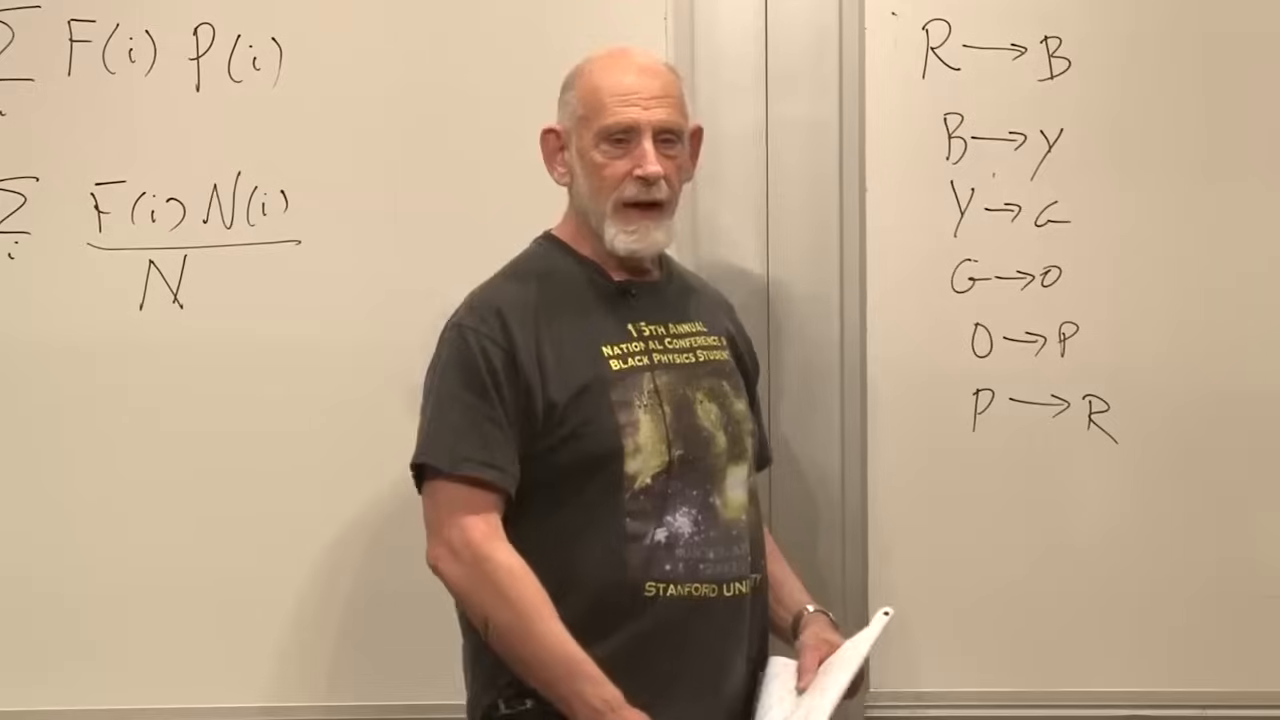
\includegraphics[width=0.92\textwidth]{lecture_01_figure_02.png}
\caption{Формулы для средних значений остаются на левой доске, а шесть детерминированных цветовых переходов перечислены на правой.}
\lectureframe{00:26:28}
\end{figure}

Список на доске становится нагляднее, если изобразить его как ориентированный цикл:
\begin{figure}[htbp]
\centering
\begin{tikzpicture}[
  >=Latex,
  state/.style={draw,circle,minimum size=8mm,inner sep=1pt}
]
\node[state] (R) at (90:2.2) {$R$};
\node[state] (B) at (30:2.2) {$B$};
\node[state] (Y) at (-30:2.2) {$Y$};
\node[state] (G) at (-90:2.2) {$G$};
\node[state] (O) at (-150:2.2) {$O$};
\node[state] (P) at (150:2.2) {$P$};
\draw[->] (R) -- (B);
\draw[->] (B) -- (Y);
\draw[->] (Y) -- (G);
\draw[->] (G) -- (O);
\draw[->] (O) -- (P);
\draw[->] (P) -- (R);
\end{tikzpicture}
\caption{Одна орбита из шести состояний. В течение каждого периода каждое состояние посещается один раз.}
\label{fig:sm1-six-cycle}
\end{figure}

Предположим, что начальное состояние нам неизвестно и что мы делаем моментальный снимок в неизвестный момент времени. Поскольку каждый шаг длится одинаково долго, система проводит одну шестую периода в каждом цвете:
\begin{equation}
 p(R)=p(B)=p(Y)=p(G)=p(O)=p(P)=\frac16.
 \label{eq:sm1-uniform-cycle}
\end{equation}
Это равенство следует не из формы объекта. Оно следует из равного времени, проводимого в состояниях.

Мы можем переставить стрелки и получить другой микроскопический закон, при этом по-прежнему образуя один цикл из шести состояний. Подробная последовательность меняется, но вероятность, получаемая по снимку, остается \(1/6\), потому что каждое состояние по-прежнему встречается один раз за период. Следовательно, для этого предсказания не нужны ни начальная точка, ни детальный порядок. Достаточно лишь структуры орбиты и равного времени каждого обновления.

\begin{classroomqa}
\classquestion{Если объект несимметричен, в каком смысле правомерно приписывать каждому цвету вероятность \(1/6\)?}
\lecturerresponse{Это приписывание является динамическим, а не геометрическим. Снимок, сделанный при неизвестной фазе шестишаговой орбиты, выбирает один из шести равных по времени интервалов. Существенная эквивалентность здесь — между положениями на орбите, а не между гранями объекта. Если бы времена пребывания были неодинаковы, то и вероятности были бы неодинаковыми.
\lecturetimestamp{00:27:11--00:29:49}}
\end{classroomqa}

\section{Несвязные циклы и сохраняющиеся величины}

Детерминистический закон не обязан помещать все состояния на одну орбиту. Рассмотрим два несвязанных цикла,
\begin{equation}
 R\longrightarrow B\longrightarrow G\longrightarrow R,
 \qquad
 P\longrightarrow Y\longrightarrow O\longrightarrow P.
 \label{eq:sm1-two-cycles}
\end{equation}
Если мы знаем, что система находится на первом цикле, то
\begin{equation}
 \begin{aligned}
 p(R)=p(B)=p(G)&=\frac13,\\
 p(P)=p(Y)=p(O)&=0.
 \end{aligned}
\end{equation}
Знание того, что она находится на втором цикле, дает обратное присвоение вероятностей.

В более общем случае требуются априорные веса. Обозначим циклы \(+1\) и \(-1\), а их вероятности — \(p_+\) и \(p_-\), причем
\begin{equation}
 p_++p_-=1.
\end{equation}
Тогда
\begin{align}
 p(R)=p(B)=p(G)&=\frac{p_+}{3},\\
 p(P)=p(Y)=p(O)&=\frac{p_-}{3}.
 \label{eq:sm1-sector-weights}
\end{align}
Множители \(1/3\) следуют из движения внутри цикла. Числа \(p_+\) и \(p_-\) — нет. Они должны следовать из дополнительного знания, возможно из другого эксперимента или из другой системы, которая выбирает начальный сектор.

Метки \(+1\) и \(-1\) задают сохраняющуюся величину: если система стартовала на одном цикле, закон обновления никогда не переводит ее на другой. Эту величину можно назвать энергией или дать ей условное имя, например \emph{зильч}. Ее название второстепенно. Сохранение означает, что пространство состояний разбивается на области, которые динамика не может пересечь.

Циклы не обязаны содержать одинаковое число состояний. Орбита из четырех состояний и орбита из двух состояний все равно задают два инвариантных сектора. Тогда выборка по равным временам дает \(1/4\) внутри первого и \(1/2\) внутри второго, причем в каждом случае это умножается на априорную вероятность соответствующего сектора. Статистическая механика должна ответить на два логически различных вопроса:
\begin{enumerate}
\item Если дан инвариантный сектор, сколько времени динамика проводит в его состояниях?
\item Какую вероятность следует приписать самому инвариантному сектору?
\end{enumerate}

\begin{classroomqa}
\audiencequestion{Предполагаем ли мы, что всем состояниям внутри одного инвариантного сектора приписывается одна и та же вероятность?}
\lecturerresponse{Для приведенных здесь дискретных модельных законов — да, потому что каждое состояние длится один и тот же интервал времени, а движение детерминистично. Неизвестной остается начальная фаза орбиты. Детектор с миллисекундным разрешением по времени не может различить микросекундные обновления, хотя достаточно быстрый снимок все же может определить, какое состояние было зафиксировано. В более общей системе неодинаковые времена пребывания нужно учитывать явно.
\lecturetimestamp{00:36:16--00:37:17}}
\end{classroomqa}

\begin{classroomqa}
\audiencequestion{Если сделаны два снимка и первый идентифицирует один цикл, должен ли второй идентифицировать тот же цикл?}
\lecturerresponse{Да. Именно это и означает сохранение. Как только измерение определяет значение сохраняющейся величины, будущие вероятности можно условить на это значение, а состояния в другом секторе получают нулевую вероятность.
\lecturetimestamp{00:37:18--00:37:45}}
\end{classroomqa}

\subsection{Энергия, распределенная между двумя системами}

Теперь заменим абстрактную метку энергией. Один изолированный ящик — это замкнутая система, и его энергия сохраняется. Два изолированных ящика имеют две независимо сохраняющиеся энергии, поскольку они не взаимодействуют. Если соединить их узким проходом, допускающим перетекание энергии, отдельные энергии могут изменяться, тогда как полная остается фиксированной.

\begin{figure}[htbp]
\centering
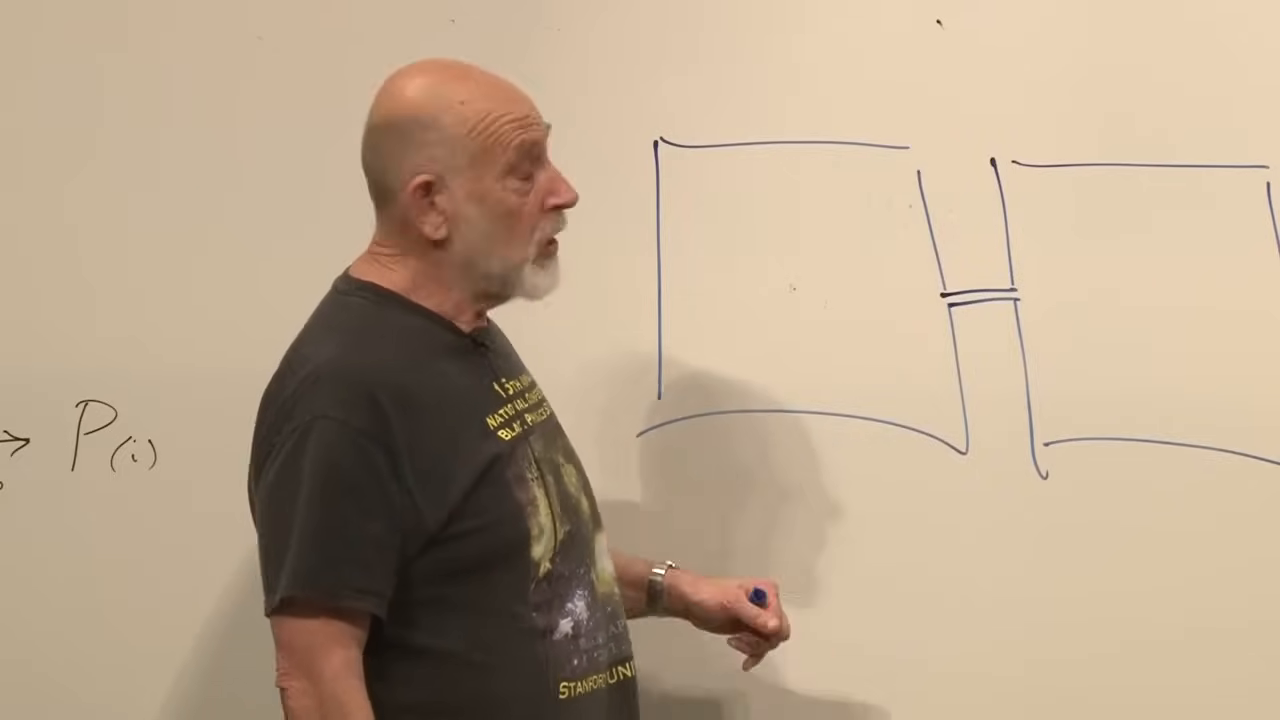
\includegraphics[width=0.92\textwidth]{lecture_01_figure_03.png}
\caption{Две подсистемы, соединенные узким каналом, через который может проходить энергия.}
\lectureframe{00:39:19}
\end{figure}

\begin{figure}[htbp]
\centering
\begin{tikzpicture}[>=Latex]
\draw[thick,rounded corners=4pt] (-4,1.8) rectangle (-0.7,-1.5);
\draw[thick,rounded corners=4pt] (0.7,1.5) rectangle (4,-1.8);
\draw[thick] (-0.7,0.45) -- (0.7,0.45);
\draw[thick] (-0.7,-0.35) -- (0.7,-0.35);
\draw[<->,very thick] (-0.45,0.05) -- (0.45,0.05);
\node at (-2.35,0.15) {subsystem \(1\)};
\node at (2.35,-0.15) {subsystem \(2\)};
\node[above] at (0,0.5) {energy exchange};
\end{tikzpicture}
\caption{После открытия соединения сохраняется только \(E_1+E_2\). Распределение энергии становится вероятностной задачей.}
\label{fig:sm1-connected-systems}
\end{figure}

При заданной полной энергии можно спросить, какова вероятность того, что подсистема \(1\) имеет \(E_1\), тогда как подсистема \(2\) имеет остаток. У одинаковых ящиков средние энергии должны быть одинаковы, но среднее не исчерпывает всего распределения. Поэтому один из способов определить вероятности для подсистемы состоит в том, чтобы вложить ее в более крупную замкнутую систему, закон сохранения которой дает недостающую информацию. Эта конструкция будет снова и снова появляться в статистической механике.

\section{Хорошие законы, плохие законы и минус первый закон}

Не всякое детерминистическое правило обновления допустимо в качестве фундаментального закона. Рассмотрим отображение
\begin{equation}
 \begin{aligned}
 R&\mapsto R,& B&\mapsto R,& Y&\mapsto R,\\
 G&\mapsto R,& O&\mapsto R,& P&\mapsto R.
 \end{aligned}
 \label{eq:sm1-all-to-red}
\end{equation}
Оно безупречно предсказывает будущее: через один шаг состояние будет красным. В обратном направлении оно не работает. Когда система находится в красном состоянии, ничто не позволяет узнать, пришла ли она из синего, желтого, зеленого, оранжевого, фиолетового или из самого красного.

\begin{figure}[htbp]
\centering
\begin{tikzpicture}[
  >=Latex,
  state/.style={draw,circle,minimum size=8mm,inner sep=1pt}
]
\node[state,fill=red!12] (R) at (0,0) {$R$};
\node[state] (B) at (-3,1.6) {$B$};
\node[state] (Y) at (-3,0) {$Y$};
\node[state] (G) at (-3,-1.6) {$G$};
\node[state] (O) at (3,1.6) {$O$};
\node[state] (P) at (3,-1.6) {$P$};
\draw[->] (B) -- (R);
\draw[->] (Y) -- (R);
\draw[->] (G) -- (R);
\draw[->] (O) -- (R);
\draw[->] (P) -- (R);
\draw[->,loop above] (R) to (R);
\end{tikzpicture}
\caption{Закон типа многие-к-одному предсказывает следующее состояние, но стирает различия между возможными прошлыми состояниями.}
\label{fig:sm1-bad-law}
\end{figure}

Напротив, замкнутый цикл сохраняет запись. Если известно прошедшее время, мы можем проследить эволюцию состояния вперед или назад, даже по прошествии многих тысяч периодов. Закон сохраняет различия между начальными условиями. Сасскинд называет это требование \emph{минус первым законом физики}: информация фундаментально не теряется.

Для конечного дискретного пространства состояний критерий по диаграмме прост:
\begin{quote}
У каждого состояния хорошего закона есть ровно одна исходящая и ровно одна входящая стрелка.
\end{quote}
Исходящая стрелка определяет будущее; входящая восстанавливает прошлое. Математически обновление — это перестановка состояний.

\subsection{Трение — лишь кажущийся контрпример}

Непрерывным аналогом служит теорема Лиувилля. Трение, по-видимому, ей противоречит. Пустите ластик скользить по столу, и, где бы он ни находился вначале, в конце концов он остановится. Схематическое уравнение сопротивления имеет вид
\begin{equation}
 m\ddot x=-\gamma\dot x,
 \qquad \gamma>0.
 \label{eq:sm1-drag}
\end{equation}
Его скорость экспоненциально убывает. Если бы это был самый фундаментальный закон для каждой частицы в герметически закрытой комнате, всякое движение затухало бы, температура падала бы до нуля, а многие начальные состояния схлопывались бы в одно конечное состояние. Закон сохранения энергии нарушался бы, информация исчезала бы, а беспорядок уменьшался бы. Это была бы непрерывная версия того, что всё приходит в красное состояние.

Реальное трение так не действует. Ластик нагревает стол, самого себя и окружающую среду. Микроскопические координаты и импульсы сохраняют различия, утраченные в видимом движении. Трение — это эффективное уравнение для подсистемы после того, как ненаблюдаемые степени свободы были отброшены; это не фундаментальный диссипативный закон для полной замкнутой системы.

\begin{classroomqa}
\classquestion{Что представляет собой дифференциальное уравнение
\(m\ddot x=-\gamma\dot x\) и почему оно не является фундаментальным законом
замкнутой системы?}
\lecturerresponse{Оно описывает вязкое сопротивление. Само по себе оно заставляет всякую скорость стремиться к нулю, что заставило бы газ остыть до нуля независимо от его начальной температуры. В реальном замкнутом описании потерянные механическая энергия и информация переходят в микроскопические степени свободы. Уравнение сопротивления надежно только после того, как эти переменные исключены из описания.
\lecturetimestamp{00:44:40--00:48:56}}
\end{classroomqa}

\section{Занятые состояния и первая энтропия}

Сохранению информации соответствует эквивалентное вероятностное утверждение. Предположим, что \(M\) из \(N\) состояний имеют одинаковую вероятность,
\begin{equation}
 p_i=
 \begin{cases}
 1/M, & i\text{ in the occupied set},\\
 0, & i\text{ outside it}.
 \end{cases}
 \label{eq:sm1-uniform-occupied}
\end{equation}
Обновление, сохраняющее информацию, может переставить, какие именно состояния заняты, но не может слить их воедино. В любой более поздний момент по-прежнему имеется \(M\) состояний с вероятностью \(1/M\). Плохое отображение \eqref{eq:sm1-all-to-red}, напротив, может схлопнуть многие занятые состояния в одно.

Число \(M\) служит мерой незнания. Если \(M=N\), возможно каждое состояние и наше незнание максимально. Если \(M=1\), микроскопическое состояние известно точно. Поэтому первое определение энтропии таково
\begin{equation}
 S=\log M.
 \label{eq:sm1-entropy-logm}
\end{equation}
Отсюда
\begin{equation}
 S_{\max}=\log N,
 \qquad
 S_{\min}=0.
\end{equation}
Если пространство состояний бесконечно, конечной верхней границы может и не быть.

В этом изложении энтропия появляется раньше температуры и даже раньше формулировки закона сохранения энергии. В этом смысле она более первична. Однако она не является свойством одной лишь механической системы. Она совместно зависит от системы и от распределения вероятностей, представляющего то, что известно. Одной и той же механической системе наблюдатели, располагающие разной информацией, могут приписывать разные энтропии.

При точной микроскопической эволюции занятые состояния лишь переставляются, поэтому эта мелкозернистая энтропия сохраняется. На практике мы теряем информацию о времени, отбрасываем корреляции и не можем отслеживать огромное число переменных. Тогда наше распределение вероятности размазывается по большему числу альтернатив, и энтропия, приписываемая грубому описанию, возрастает. Чтобы пригодное нам описание теряло информацию, вовсе не требуется, чтобы уравнения её уничтожали.

\begin{classroomqa}
\classquestion{Какова максимально возможная энтропия конечной системы с \(N\) состояниями?}
\lecturerresponse{Она равна \(\log N\) и достигается, когда все \(N\) состояний равновероятны. Наименьшая энтропия равна нулю; она достигается, когда вероятность одного состояния равна единице. Следовательно, энтропия характеризует как состояние знания, так и доступное пространство состояний.
\lecturetimestamp{00:56:46--00:58:19}}
\end{classroomqa}

\section{Поток Лиувилля в непрерывном фазовом пространстве}

Для частиц с непрерывными координатами и импульсами микроскопическое состояние есть точка в фазовом пространстве. Координаты мы обозначаем как \(q_a\), а сопряжённые им импульсы — как \(p_a\). Для многих частиц осей оказывается чрезвычайно много; двумерный рисунок, где есть лишь одна \(q\) и один \(p\), служит только условной иллюстрацией. Размерность фазового пространства чётна, потому что каждой координате соответствует сопряжённый импульс.

Предположим, что наше знание представлено областью \(\Omega_0\): плотность вероятности внутри этой области постоянна, а вне её равна нулю. Например, знание того, что каждая частица находится в комнате, ограничивает координаты положения, тогда как ограничения на их скорости ограничивают импульсные координаты.

Гамильтонова эволюция переносит каждую точку фазового пространства вдоль траектории. Близкие точки переходят в близкие точки, и занятая область течёт как порция несжимаемой жидкости:
\begin{figure}[htbp]
\centering
\begin{tikzpicture}[>=Latex,scale=0.95]
\draw[->] (-4.2,0) -- (4.3,0) node[right] {$q$};
\draw[->] (-3.7,-2.2) -- (-3.7,2.4) node[above] {$p$};
\draw[fill=blue!12,thick]
  (-3.0,-0.5) .. controls (-2.7,1.0) and (-1.3,1.2) .. (-0.9,0.1)
  .. controls (-0.6,-1.0) and (-2.2,-1.4) .. cycle;
\node at (-1.9,0.0) {$\Omega_0$};
\draw[->,very thick] (-0.3,0.2) -- (0.8,0.2);
\draw[fill=orange!15,thick]
  (1.2,-1.1) .. controls (1.5,0.3) and (2.3,1.8) .. (3.2,1.1)
  .. controls (3.6,0.7) and (2.8,-0.4) .. (2.5,-1.5)
  .. controls (2.1,-1.8) and (1.5,-1.6) .. cycle;
\node at (2.35,0.1) {$\Omega_t$};
\end{tikzpicture}
\caption{Гамильтонов поток может растягивать и сдвигать занятую область фазового пространства, но сохраняет её объём.}
\label{fig:sm1-liouville-flow}
\end{figure}

Теорема Лиувилля утверждает:
\begin{equation}
 \operatorname{Vol}(\Omega_t)
 =
 \operatorname{Vol}(\Omega_0).
 \label{eq:sm1-liouville-volume}
\end{equation}
Если начальная плотность равномерна на \(\Omega_0\), то перенесённая плотность равномерна на \(\Omega_t\). Это непрерывный аналог сохранения числа и весов занятых дискретных состояний.

Эта теорема также геометрически разрешает загадку трения. Если смотреть только на наблюдаемый импульс ластика, облако возможностей как будто сжимается к \(p=0\). В полном фазовом пространстве это облако распространяется по координатам и импульсам молекул в ластике и столе. Проекция может сжиматься, тогда как полный многомерный объём остаётся постоянным.

\begin{classroomqa}
\classquestion{Если каждая наблюдаемая траектория стремится к покою, схлопнулась ли занятая область фазового пространства на ось \(p=0\)?}
\lecturerresponse{Только в редуцированной проекции. Полная система включает микроскопические переменные стола, ластика и окружающей среды. По мере того как диапазон видимого импульса сужается, распределение растекается по этим скрытым направлениям. Теорема Лиувилля относится к полному замкнутому фазовому пространству, а не к неполному набору макроскопических переменных.
\lecturetimestamp{01:04:37--01:06:29}}
\end{classroomqa}

\section{От минус первого закона к первому закону}

\subsection{Кратко о нулевом законе}

Прежде чем формулировать первый закон, полезно назвать нулевой. Тепловое равновесие ещё не определено, поэтому пока этот закон является лишь структурным утверждением:
\begin{quote}
Если система \(A\) находится в тепловом равновесии с \(B\), а \(B\) находится в тепловом равновесии с \(C\), то \(A\) находится в тепловом равновесии с \(C\).
\end{quote}
Эта транзитивность позже сделает возможным введение температуры. Пока же мы оставим её в стороне.

\subsection{Сохранение энергии}

Первый закон для замкнутой системы просто гласит:
\begin{equation}
 \frac{dE}{dt}=0.
 \label{eq:sm1-first-law}
\end{equation}
Его компактная форма скрывает его силу. Энергия является сохраняющейся величиной, и слово энергия позже приобретёт более содержательный термодинамический смысл.

Если замкнутая система состоит из двух частей и их энергии аддитивны,
\begin{equation}
 E=E_1+E_2,
\end{equation}
то
\begin{equation}
 \frac{dE_1}{dt}+\frac{dE_2}{dt}=0,
 \qquad\text{or}\qquad
 \frac{dE_1}{dt}=-\frac{dE_2}{dt}.
 \label{eq:sm1-energy-exchange}
\end{equation}
Вторая форма делает обмен явным: энергия, потерянная одной подсистемой, приобретается другой.

Предположение об аддитивности требует осторожности. У двух гравитационно взаимодействующих частиц есть индивидуальные кинетические энергии, но их взаимодействие даёт потенциальную энергию, принадлежащую паре. Полная энергия сохраняется, хотя её нельзя точно записать как энергию одного тела плюс энергию другого.

Термодинамика часто допускает превосходное аддитивное приближение, потому что объёмная энергия масштабируется с объёмом, тогда как энергия короткодействующего взаимодействия между большими соседними частями масштабируется главным образом с площадью их соприкосновения. Разделите большой стол на блоки: внутренняя энергия каждого блока — объёмный эффект, а взаимодействие между соседними блоками — поверхностный эффект. Для больших блоков этот вклад сравнительно мал. Уравнение
\eqref{eq:sm1-first-law} точно для замкнутого целого; форма для подсистем
\eqref{eq:sm1-energy-exchange} предполагает пренебрежимо малую энергию взаимодействия.

\begin{classroomqa}
\audiencequestion{Нормировка \(\sum_i p_i=1\) также предполагает, что перечисленные исходы взаимно исключают друг друга?}
\lecturerresponse{Да. Метка состояния определяется так, чтобы альтернативы не перекрывались: если игральная кость находится в жёлтом состоянии, то она не находится одновременно в красном состоянии. В обычном языке цвета могут смешиваться, но разбиение на состояния, используемое при вычислении вероятности, должно состоять из взаимно исключающих альтернатив.
\lecturetimestamp{01:12:14--01:12:55}}
\end{classroomqa}

\section{Возвращение к энтропии}

Теперь лекция явно возвращается к тому, что осталось незавершённым. Температура, хотя и знакома нашим чувствам, является производной величиной. Прежде чем можно будет чётко определить температуру, должны быть введены энтропия и энергия.

\subsection{Общие распределения вероятности}

Специальное определение \(S=\log M\) применимо, когда \(M\) состояний равновероятны, а все остальные имеют нулевую вероятность. Общее распределение не обязано иметь прямоугольную форму. Его веса могут изменяться по меткам состояний плавно или нерегулярно.

\begin{figure}[htbp]
\centering
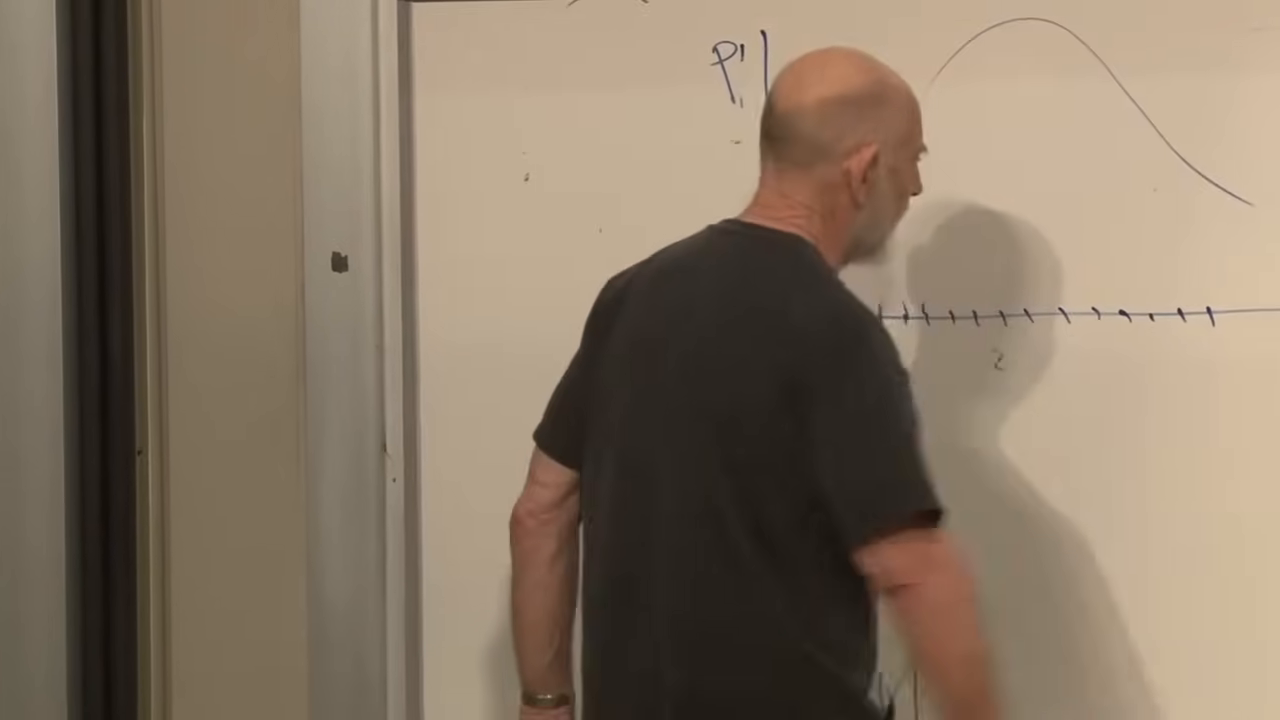
\includegraphics[width=0.92\textwidth]{lecture_01_figure_05.png}
\caption{Распределение вероятности по дискретным меткам состояний. Для энтропии важен разброс, а не точная форма кривой.}
\lectureframe{01:14:40}
\end{figure}

\begin{figure}[htbp]
\centering
\resizebox{\linewidth}{!}{%
\begin{tikzpicture}[>=Latex,scale=0.93]
\draw[->] (-4.2,0) -- (4.4,0) node[right] {state label \(i\)};
\draw[->] (-4,0) -- (-4,3.2) node[above] {$p_i$};
\foreach \x in {-3.6,-3.1,...,3.6}
  \draw (\x,0.08) -- (\x,-0.08);
\draw[very thick]
  plot[smooth] coordinates {
  (-3.7,0.12) (-3.0,0.28) (-2.3,0.72) (-1.6,1.45)
  (-0.9,2.25) (-0.2,2.65) (0.5,2.28) (1.2,1.55)
  (1.9,0.88) (2.7,0.38) (3.5,0.14)};
\draw (-1.8,-0.18) -- (-1.8,-0.5);
\draw (1.8,-0.18) -- (1.8,-0.5);
\draw[<->] (-1.8,-0.46) -- (1.8,-0.46);
\node at (0,-0.82) {effective spread};
\end{tikzpicture}
}
\caption{Узкое распределение несёт меньшую неопределённость, чем широкое. Энтропия должна характеризовать распределение в целом.}
\label{fig:sm1-probability-spread}
\end{figure}

Общее определение имеет вид
\begin{equation}
 S=-\sum_i p_i\log p_i.
 \label{eq:sm1-shannon-entropy}
\end{equation}
Используя \eqref{eq:sm1-expectation}, получаем
\begin{equation}
 S=-\langle\log p\rangle.
\end{equation}
Знак минус компенсирует тот факт, что \(\log p_i<0\), когда \(0<p_i<1\).

\subsection{Восстановление результата для равномерного случая}

Нужно проверить, что общая формула воспроизводит первое определение. Для незанятого состояния \(p_i=0\), тогда как \(\log p_i\) расходится. Однако произведение имеет хорошо определённое предельное значение
\begin{equation}
 \lim_{p\to0^+}p\log p=0.
 \label{eq:sm1-plogp-limit}
\end{equation}
Следовательно, состояния с нулевой вероятностью не вносят никакого вклада.

\begin{classroomqa}
\audiencequestion{Если \(p_i=0\), неужели этот член действительно обращается в нуль? Логарифм нуля равен минус бесконечности.}
\lecturerresponse{Этот член определяется пределом
\(\lim_{p\to0^+}p\log p\), который равен нулю. Множитель \(p\) стремится к нулю быстрее, чем логарифм расходится. Поэтому сколь угодно маловероятные состояния дают сколь угодно малые вклады, а точно невозможное состояние не даёт никакого вклада.
\lecturetimestamp{01:18:27--01:19:46}}
\end{classroomqa}

Для каждого из \(M\) занятых состояний \(p_i=1/M\). Следовательно,
\begin{align}
 S
 &=-\sum_{\mathrm{occupied}\ i}
 \frac1M\log\!\left(\frac1M\right)\\
 &=-M\frac1M\log\!\left(\frac1M\right)\\
 &=-\log\!\left(\frac1M\right)
 =\log M.
 \label{eq:sm1-entropy-check}
\end{align}
Общее выражение в точности совпадает со специальным. Более широкое распределение придаёт заметный вес большему числу альтернатив и потому имеет большую энтропию; более узкое распределение имеет меньшую энтропию.

\begin{figure}[htbp]
\centering
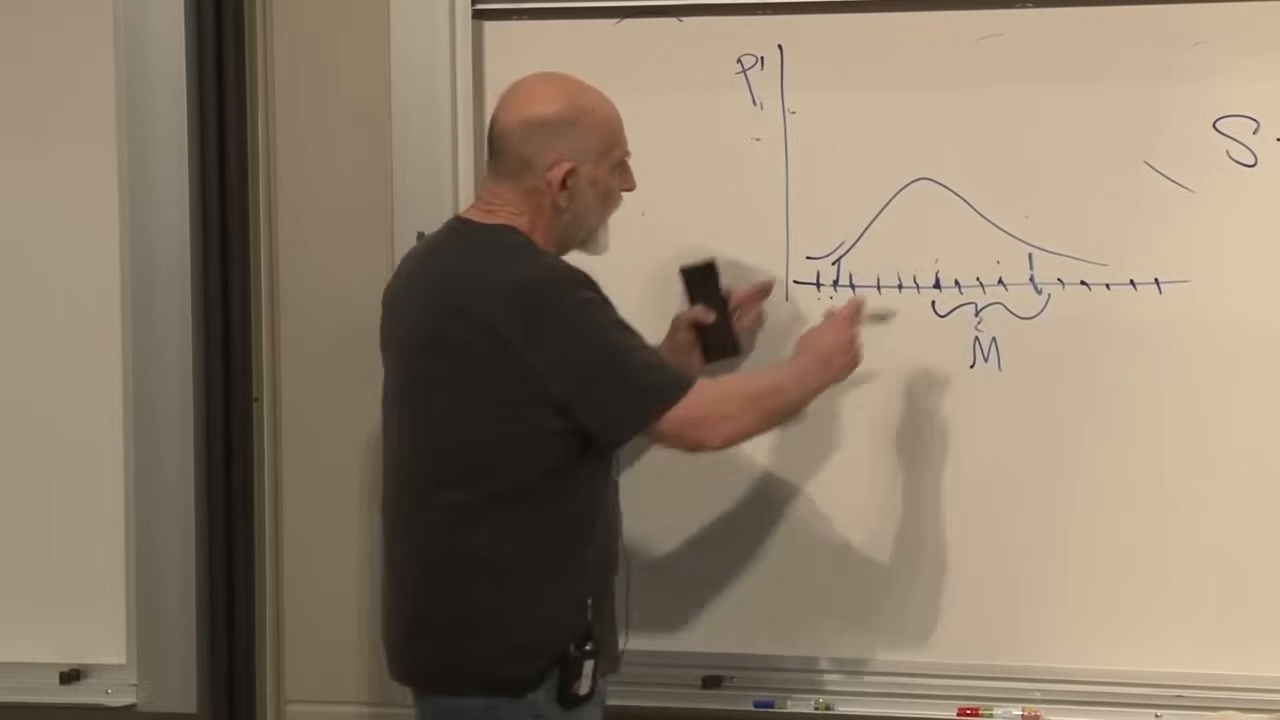
\includegraphics[width=0.92\textwidth]{lecture_01_figure_06.png}
\caption{Отмеченная ширина \(M\) подчёркивает связь между разбросом значимых вероятностей и энтропией.}
\lectureframe{01:16:42}
\end{figure}

Энтропия относится к распределению вероятности на пространстве состояний. Это не самостоятельная наблюдаемая величина, такая как энергия или импульс одного микросостояния. Точное состояние можно представить распределением, сосредоточенным на этом состоянии; тогда энтропия равна нулю, но при изменении состояния знания она меняется.

\section{Монеты, биты и явный подсчёт}

Пусть \(n\) — число монет. Число микроскопических конфигураций равно
\begin{equation}
 N=2^n.
 \label{eq:sm1-coin-state-count}
\end{equation}
Если о монетах ничего не известно, все \(2^n\) конфигурации равновероятны, и
\begin{equation}
 S_{\max}=\log(2^n)=n\log2.
 \label{eq:sm1-coin-max-entropy}
\end{equation}
Энтропия аддитивна по числу независимых монет.

При логарифмах по основанию \(2\) система с двумя состояниями, о которой ничего не известно, имеет энтропию в один бит. При натуральных логарифмах её энтропия равна \(\log2\). Единица измерения условна; лежащие в основе порядок и аддитивность не меняются.

В противоположном предельном случае, если состояние каждой монеты известно, ровно одна конфигурация имеет вероятность единица:
\begin{equation}
 S=0.
\end{equation}
Чем больше известно, тем меньше энтропия.

Теперь предположим, что ровно одна из \(n\) монет показывает решку, а все остальные — орла, причём положение решки неизвестно. Имеется \(n\) равновероятных конфигураций, по одной для каждого возможного положения решки, так что
\begin{equation}
 S=\log n.
 \label{eq:sm1-one-tail-entropy}
\end{equation}
Вообще говоря, это не целое кратное \(\log2\). Бит — удобная единица, а не утверждение, что любая энтропия бывает только целым числом бит.

\begin{classroomqa}
\audiencequestion{Появляется ли \(\log2\) только потому, что у каждой монеты есть два возможных состояния? Дал бы элемент с тремя состояниями \(\log3\)?}
\lecturerresponse{Именно. Элемент с \(k\) возможными состояниями, о котором известно лишь то, что все они равновероятны, даёт вклад \(\log k\). Двоичные переключатели особенно удобны в компьютерах, потому что физические переключатели естественным образом реализуют два устойчивых состояния и потому что 2 — наименьшее нетривиальное целое число.
\lecturetimestamp{01:29:55--01:30:48}}
\end{classroomqa}

\begin{classroomqa}
\audiencequestion{Какое основание логарифма здесь имеется в виду?}
\lecturerresponse{В этих физических формулах \(\log\) означает натуральный логарифм. Специалисты по теории информации часто используют основание \(2\), так что энтропия измеряется непосредственно в битах. Смена основания умножает любую энтропию на один и тот же постоянный коэффициент пересчёта и не меняет ни одного физического вывода.
\lecturetimestamp{01:30:49--01:32:06}}
\end{classroomqa}

\section{Энтропия в непрерывном фазовом пространстве}

Вернёмся к классическому фазовому пространству \(\Gamma\). Если плотность вероятности равномерна в области объёма \(V_\Gamma\) и вне её равна нулю, то аналог подсчёта \(M\) равновероятных состояний имеет вид
\begin{equation}
 S=\log\!\left(\frac{V_\Gamma}{V_0}\right).
 \label{eq:sm1-continuous-uniform}
\end{equation}
Здесь \(V_\Gamma\) — это объём в полном многомерном пространстве координат и импульсов, а не обычный пространственный объём. Фиксированный объём \(V_0\) — это эталонная ячейка фазового пространства, делающая логарифм безразмерным. При \(V_0=1\) получаем сокращённую запись \(S=\log V_\Gamma\), использовавшуюся на доске.

Для общей плотности вероятности \(P(q,p)\) дискретная сумма переходит в интеграл по фазовому пространству. Нормировка имеет вид
\begin{equation}
 \int_\Gamma d\Gamma\,P(q,p)=1,
 \label{eq:sm1-continuous-normalization}
\end{equation}
а энтропия равна
\begin{equation}
 S=-\int_\Gamma d\Gamma\,
 P(q,p)\log\!\bigl[P(q,p)V_0\bigr].
 \label{eq:sm1-continuous-entropy}
\end{equation}
Плотность — это вероятность, приходящаяся на ячейку фазового пространства. Концептуально \eqref{eq:sm1-continuous-entropy} по-прежнему измеряет, насколько широко распределена вероятность; для равномерной области она сводится к логарифму занятого объёма, измеренного в единицах эталонной ячейки. Замена этой фиксированной ячейки сдвигает любую непрерывную энтропию на одну и ту же аддитивную постоянную и оставляет разности энтропий неизменными.

\begin{classroomqa}
\audiencequestion{Почему обозначение координаты изменилось с \(x\) на \(q\)?}
\lecturerresponse{Никакого физического изменения нет. В классической механике для координат обычно используют либо \(x\), либо \(q\), а для сопряжённых импульсов — \(p\). Смена обозначения была лишь оговоркой; построение фазового пространства остаётся тем же.
\lecturetimestamp{01:37:10--01:37:39}}
\end{classroomqa}

Температура и распределение Больцмана намеренно отложены. Следующей задачей будет определить тепловое равновесие, а затем установить соответствующее ему распределение вероятностей.

\section{Вопросы о корреляции, аддитивности и информации}

\subsection{Корреляция означает, что одно измерение меняет распределение вероятностей для другой величины}

Полное незнание о независимых монетах приписывает каждой конфигурации равную вероятность. Измерение одной монеты тогда ничего не сообщает ни о какой другой монете. Их распределения остаются неизменными.

Ансамбль с одной решкой устроен иначе. Если у измеренной монеты выпала решка, то у всех остальных наверняка орёл. Если у измеренной монеты выпал орёл, то единственная решка должна находиться среди оставшихся \(n-1\) монет, так что каждая из оставшихся позиций имеет условную вероятность
\begin{equation}
\begin{aligned}
 p(&\text{tail at a specified remaining position}\\
   &\mid\text{measured head})=\frac{1}{n-1}.
\end{aligned}
 \label{eq:sm1-conditional-tail}
\end{equation}
Это и есть корреляция: узнав одну переменную, мы меняем распределение вероятностей, приписываемое другой.

\begin{classroomqa}
\audiencequestion{Предполагалась ли независимость монет в примерах с энтропией?}
\lecturerresponse{Только тогда, когда полное незнание представлялось равными вероятностями для всех \(2^n\) конфигураций. В этом случае измерение одной монеты не меняет распределений остальных. Пример с одной решкой явно коррелирован: измерение уточняет, что возможно в других местах. Указанная информация определяет, какое распределение вероятностей используется.
\lecturetimestamp{01:38:43--01:41:58}}
\end{classroomqa}

Пример с несвязанными циклами имеет ту же логическую форму. Измерение сохраняющейся метки \(+1\) или \(-1\) ограничивает все последующие состояния одним сектором. Условление по сохраняющейся информации изменяет допустимое распределение.

Энтропия аддитивна для некоррелированных систем. Если
\begin{equation}
 p_{ij}=p_i^{(A)}p_j^{(B)},
\end{equation}
то
\begin{align}
 S_{AB}
 &=-\sum_{i,j}p_i^{(A)}p_j^{(B)}
 \log\!\left[p_i^{(A)}p_j^{(B)}\right]\\
 &=S_A+S_B.
 \label{eq:sm1-entropy-additivity}
\end{align}
Корреляции препятствуют такой факторизации и уменьшают независимую неопределённость пары.

В качестве упражнения представьте себе ряд двоичных переменных, для которых верхнее состояние означает, что каждый сосед с вероятностью три четверти находится в нижнем состоянии. Измерение в одном узле немедленно изменяет то, что известно о ближайших узлах. Такое распределение коррелировано, и его энтропию нельзя найти, просто складывая изолированные одноузловые энтропии без учёта этих корреляций.

\subsection{Больцман, Шеннон и квантовая неопределённость}

\begin{classroomqa}
\audiencequestion{Как более ранняя термодинамическая энтропия связана с информационно-теоретической энтропией Шеннона?}
\lecturerresponse{В обоих случаях появляется одна и та же функциональная форма:
\(-\sum_i p_i\log p_i\). Шеннон обычно использовал основание \(2\), тогда как физики обычно используют натуральные логарифмы и восстанавливают постоянную Больцмана, когда энтропия выражается в термодинамических единицах. Математическое различие сводится лишь к постоянному коэффициенту пересчёта, хотя физические вопросы, задающие вероятности, могут быть очень разными.
\lecturetimestamp{01:44:05--01:46:06}}
\end{classroomqa}

Для равновероятных микросостояний термодинамическую формулу часто записывают в виде
\begin{equation}
 S_{\mathrm{thermo}}=k_{\mathrm B}\log W,
 \label{eq:sm1-boltzmann-formula}
\end{equation}
где \(W\) — число доступных микросостояний. В единицах, где \(k_{\mathrm B}=1\), это в точности \(S=\log W\). Постоянная Больцмана служит коэффициентом пересчёта между единицами температуры и единицами энергии; естественный микроскопический масштаб температуры — энергия.

\begin{classroomqa}
\audiencequestion{Является ли эта энтропия просто иной формой принципа неопределённости Гейзенберга?}
\lecturerresponse{Нет. Рассматриваемая здесь энтропия измеряет неопределённость в распределении вероятностей по возможным состояниям. На языке квантовой механики это неопределённость смешанного состояния, а не внутренняя неопределённость измерения, которая может сохраняться даже для чистого состояния. Эти два понятия необходимо различать.
\lecturetimestamp{01:46:07--01:47:31}}
\end{classroomqa}

\section{Что было установлено}

Исходным пунктом была не случайность в самих законах. Детерминистическая динамика в сочетании с неполным знанием начального состояния уже порождает вероятности. Одна орбита задаёт веса через время пребывания в каждом состоянии; несвязанные орбиты выявляют сохраняющиеся величины и требуют априорных весов между секторами. Допустимые микроскопические законы сохраняют различимость состояний; в конечном пространстве состояний это означает по одной входящей и по одной исходящей стрелке в каждом состоянии, а в непрерывной механике выражается теоремой Лиувилля.

Эта структура приводит сначала к
\begin{equation}
 S=\log M
\end{equation}
для \(M\) занятых равновероятных состояний, затем к
\begin{equation}
 S=-\sum_i p_i\log p_i,
\end{equation}
и наконец к его интегралу по фазовому пространству. Энтропия фиксирует распределение вероятностей и, следовательно, состояние знания. Детальная информация сохраняется микроскопическим законом даже тогда, когда практическое огрублённое описание теряет её из виду.

Сохранение энергии даёт первый закон, тогда как аддитивность энергий подсистем требует пренебрежимо малой энергии взаимодействия. Энтропия аддитивна при аналогичном условии: распределения вероятностей подсистем должны быть некоррелированными. Эти два вида аддитивности подготавливают следующий шаг, на котором тепловое равновесие, температура и распределение Больцмана свяжут энергию с вероятностью.
\chapter{Температура через энтропию и энергию}

\lectureoverview{Температура сначала возникает как перевод привычных человеку термометрических единиц в микроскопические единицы энергии. После соответствующего перевода термодинамической энтропии в безразмерную статистическую энтропию мы описываем равновесие как однопараметрическое семейство распределений вероятностей. Производная \(dE/dS\) тогда определяет температуру, а первые два закона показывают, почему разность температур определяет направление потока энергии.}

\section{Коэффициенты пересчёта и единицы человеческого масштаба}

Многие физические константы служат коэффициентами пересчёта. Скорость света позволяет перевести расстояние во время:
\begin{equation}
 t=\frac{x}{c}.
\end{equation}
Если расстояния и времена измеряются в согласованных единицах, можно положить \(c=1\). Никакой физический эффект не исчезает; два вида измерения просто приведены к общей шкале.

Постоянная Больцмана имеет тот же характер. Она переводит температуру, считываемую по термометру человеческого масштаба, в энергию. Прилагательное \emph{человеческого масштаба} важно. Такие единицы выбирают потому, что макроскопические приборы могут их воспроизводить и различать, а не потому, что микроскопическая динамика выделяет именно их.

Градус Цельсия был зафиксирован делением интервала между точками замерзания и кипения воды при стандартном давлении на 100 частей. В шкале Кельвина используется градус той же величины, но нуль помещается в абсолютный нуль. Выбор другого вещества, другого интервала или градусов Фаренгейта изменил бы числа, но не физику.

\begin{classroomqa}
\audiencequestion{Разве шкала Фаренгейта не была создана ещё в XVII веке?}
\lecturerresponse{Точная дата здесь не нужна. Существенно то, что все такие шкалы конструировались вокруг температур, которые люди могли получать и измерять. Размер их градуса задаётся соглашением, а не микроскопической физикой.
\lecturetimestamp{00:01:34--00:01:50}}
\end{classroomqa}

В то время, когда создавались эти шкалы, молекулярное происхождение тепла было недоступно эксперименту. Изменение на 1 градус можно было наблюдать с помощью макроскопического термометра, тогда как энергию одной молекулы измерить было нельзя. Поэтому было естественно ввести единицу температуры прежде, чем кто-либо узнал, что по своей сути температура есть энергетическая шкала.

\section{Почему температура имеет единицы энергии}

Рассмотрим разреженный одноатомный газ. Разреженный означает, что для настоящей цели энергиями взаимодействия между молекулами можно пренебречь. В тепловом равновесии принцип равнораспределения приписывает каждой квадратичной поступательной степени свободы энергию, равную произведению постоянной Больцмана и \(T_{\mathrm K}/2\). В трёх пространственных измерениях,
\begin{equation}
 \left\langle E_{\mathrm{kin}}\right\rangle
 =\frac{3}{2}k_{\mathrm B}T_{\mathrm K}.
 \label{eq:sm2-equipartition-kelvin}
\end{equation}
Множитель 3 учитывает движение в направлениях \(x\), \(y\) и \(z\). Множитель 1/2 возникает из квадратичной кинетической энергии.

Это соотношение не ограничивается одним видом частиц. В смеси гелия и кислорода в равновесии каждая свободно перемещающаяся частица имеет одну и ту же среднюю кинетическую энергию движения центра масс, хотя более тяжёлые частицы движутся медленнее. Поскольку
\begin{equation}
 E_{\mathrm{kin}}=\frac{1}{2}mv^2,
\end{equation}
из одинаковой характерной энергии следует \(v\propto m^{-1/2}\).

Эту же идею можно довести до намеренно крайнего примера. Подвесьте шар для боулинга в текучей среде и дайте всей системе прийти к равновесию. Его броуновские поступательные степени свободы определяются той же энергетической шкалой, что и у молекулы. Скорость шара фантастически меньше, потому что его масса фантастически больше, но температура сравнивает энергетические шкалы, а не скорости.

При комнатной температуре \(T_{\mathrm K}\) составляет примерно \(300\,\mathrm K\), тогда как энергия одной микроскопической степени свободы в джоулях очень мала. Поэтому коэффициент пересчёта мал:
\begin{equation}
 k_{\mathrm B}\simeq 1.38\times10^{-23}\,
 \mathrm{J\,K^{-1}}.
 \label{eq:sm2-boltzmann-value}
\end{equation}
Его порядок величины связан с числом Авогадро, а не является случайным совпадением:
\begin{equation}
 R=N_{\mathrm A}k_{\mathrm B}.
\end{equation}
Газовая постоянная \(R\) описывает моль, тогда как \(k_{\mathrm B}\) описывает соответствующий масштаб на одну микроскопическую составляющую.

В фундаментальных формулах снова и снова встречается комбинация \(k_{\mathrm B}T_{\mathrm K}\). Поэтому удобнее определить
\begin{equation}
 T\equiv k_{\mathrm B}T_{\mathrm K}.
 \label{eq:sm2-energy-temperature}
\end{equation}
Отныне сама \(T\) имеет единицы энергии, а
\eqref{eq:sm2-equipartition-kelvin} принимает вид
\begin{equation}
 \left\langle E_{\mathrm{kin}}\right\rangle=\frac{3}{2}T.
 \label{eq:sm2-equipartition-natural}
\end{equation}
Если энергия измеряется в джоулях, то температура измеряется в джоулях. Если энергия измеряется в электрон-вольтах, то температура измеряется в электрон-вольтах. Никакой новой природной единицы, называемой единицей температуры, не существует.

\section{Два соглашения об энтропии}

Тот же перевод возникает и на стороне энтропии. Макроскопическая термодинамика выросла из анализа тепловых машин. Карно дал решающие рассуждения о тепловых машинах; Клаузиус позже ввёл термодинамическую энтропию и обозначение \(S\). В используемых здесь обозначениях назовём эту макроскопическую величину \(S_{\mathrm C}\). Её единицы — энергия, делённая на термометрическую температуру, например джоули на кельвин.

Статистическая энтропия безразмерна. Для дискретного распределения,
\begin{equation}
 S=-\sum_i p_i\log p_i.
 \label{eq:sm2-statistical-entropy}
\end{equation}
При натуральных логарифмах равновероятная бинарная альтернатива имеет энтропию \(\log2\); при логарифмах по основанию 2 та же величина называется одним битом. Эти два соглашения об энтропии связаны соотношением
\begin{equation}
 S=\frac{S_{\mathrm C}}{k_{\mathrm B}},
 \qquad
 S_{\mathrm C}=k_{\mathrm B}S.
 \label{eq:sm2-entropy-conversion}
\end{equation}
Макроскопическому значению, скромному в \(\mathrm{J\,K^{-1}}\), соответствует огромная безразмерная энтропия, потому что она подсчитывает информацию, распределённую по огромному числу микроскопических составляющих.

Уравнения \eqref{eq:sm2-energy-temperature} и
\eqref{eq:sm2-entropy-conversion} устанавливают используемое далее соглашение:
\[
 [T]=[\text{energy}],
 \qquad
 [S]=1.
\]
Теперь постоянная Больцмана может исчезнуть из рабочих формул. Её всегда можно восстановить, заменив \(T\) на \(k_{\mathrm B}T_{\mathrm K}\), а
\(S\) на \(S_{\mathrm C}/k_{\mathrm B}\).

\begin{classroomqa}
\audiencequestion{Если не считать множителя \(3/2\), не является ли новая температура просто энергией, измеряемой в джоулях?}
\lecturerresponse{Да, если в качестве единицы энергии выбраны джоули. Джоуль — это единица МКС \(\mathrm{kg\,m^2\,s^{-2}}\). Вместо этого можно использовать электрон-вольты или любую другую единицу энергии; тогда температура должна выражаться в той же единице. Множитель \(3/2\) относится к примеру идеального газа, а не к определению температуры.
\lecturetimestamp{00:15:49--00:16:45}}
\end{classroomqa}

\begin{classroomqa}
\audiencequestion{Если на доске указаны кельвины, разве \(k_{\mathrm B}\) тогда не является определённой константой?}
\lecturerresponse{Она определена после того, как заданы и единицы температуры, и единицы энергии. Замените кельвины на градусы Фаренгейта или джоули на электрон-вольты, и её численное значение изменится. Эта зависимость от единиц и есть именно поведение коэффициента пересчёта.
\lecturetimestamp{00:16:46--00:18:33}}
\end{classroomqa}

\begin{classroomqa}
\audiencequestion{Определяется ли численное значение постоянной Больцмана экспериментально?}
\lecturerresponse{Да. Исторически для её оценки требовалась микроскопическая информация об атомах и об их численной плотности. Больцман понял связь между молекулярной энергией и температурой ещё до того, как эти величины стали известны точно, примерно так же, как Ньютон понимал роль гравитационной постоянной до того, как её точно измерили.
\lecturetimestamp{00:18:46--00:20:00}}
\end{classroomqa}

\section{Равновесие — статистическое состояние}

Один лишь перевод единиц всё ещё не определяет температуру. Прикосновение к чему-то горячему даёт полезную биологическую интуицию, но температура — это производная физическая величина, построенная из энергии и энтропии.

Представьте себе систему, находящуюся в контакте с большой средой, чьи макроскопические условия фиксированы. Между ними может проходить энергия. Если у системы изначально слишком много энергии, она в среднем теряет энергию; если слишком мало, то в среднем получает её. В тепловом равновесии микроскопические обмены продолжаются, но ни в одном направлении нет среднего результирующего потока.

Пусть \(i\) обозначает точное микроскопическое состояние системы, а \(E_i\) — энергию этого состояния. Равновесие не означает, что система застывает в одном состоянии. Её взаимодействие со средой непрерывно меняет микросостояние, поэтому каждой возможности мы приписываем вероятность \(P_i\). Основные соотношения таковы:
\begin{align}
 \sum_i P_i &=1,
 \label{eq:sm2-normalization}\\
 \sum_i P_iE_i &=\overline E,
 \label{eq:sm2-mean-energy}\\
 S&=-\sum_iP_i\log P_i.
 \label{eq:sm2-equilibrium-entropy}
\end{align}
Черта над \(\overline E\) подчёркивает, что энергия подсистемы флуктуирует. Одно измерение может дать одно значение, а следующее — другое; повторные измерения приводят к распределению, среднее которого задаётся \eqref{eq:sm2-mean-energy}.

\begin{figure}[t]
\centering
\includegraphics[width=0.82\textwidth]{lecture_02_figure_02.png}
\caption{Нормировка и средняя энергия на доске: \(\sum_iP(i)=1\) и \(\sum_iP(i)E(i)=\langle E\rangle\).}
\lectureframe{00:24:10}
\end{figure}

\section{Семейство, параметризованное средней энергией}

Равновесное распределение сильно зависит от средней энергии. Поставьте кастрюлю с водой на плиту, и \(\overline E\) возрастёт; поставьте её в снег, и \(\overline E\) уменьшится. При этом меняются и вероятности. Поэтому равновесие следует рассматривать не как одно распределение, а как однопараметрическое семейство:
\begin{equation}
 P_i(\overline E).
 \label{eq:sm2-family}
\end{equation}
Каждый его член удовлетворяет
\begin{align}
 \sum_iP_i(\overline E)&=1,
 \label{eq:sm2-family-normalization}\\
 \sum_iP_i(\overline E)E_i&=\overline E.
 \label{eq:sm2-family-mean}
\end{align}

\begin{figure}[t]
\centering
\includegraphics[width=0.88\textwidth]{lecture_02_figure_03.png}
\caption{Переход к \(P(i,\overline E)\). Ранее записанные уравнения нормировки, средней энергии и энтропии остаются видимыми, пока вводится семейство распределений.}
\lectureframe{00:26:29}
\end{figure}

Для схематического графика упорядочим состояния по возрастанию \(E_i\). Тогда горизонтальную ось можно читать либо как индекс \(i\), либо как соответствующую энергию. Более высокая средняя энергия смещает вероятностный вес к состояниям, расположенным дальше вправо. Каждая кривая должна сохранять полную площадь, равную единице.

\begin{figure}[t]
\centering
\includegraphics[width=0.88\textwidth]{lecture_02_figure_04.png}
\caption{Несколько схематических распределений \(P(i,\overline E)\). Кривые, у которых вес сильнее смещен вправо, имеют большую среднюю энергию, при этом каждое распределение остается нормированным.}
\lectureframe{00:28:40}
\end{figure}

\begin{figure}[t]
\centering
\begin{tikzpicture}[x=1cm,y=1cm]
\draw[->] (0,0) -- (7.4,0) node[right] {$E_i$};
\draw[->] (0,0) -- (0,3.25) node[above] {$P_i(\overline E)$};
\draw[thick,blue!70!black]
  plot[smooth] coordinates {(0,0) (0.35,1.6) (0.85,2.65) (1.45,1.45)
  (2.2,0.35) (3.0,0)};
\draw[thick,teal!70!black]
  plot[smooth] coordinates {(0,0) (0.7,0.7) (1.5,1.7) (2.5,2.0)
  (3.7,0.8) (4.8,0)};
\draw[thick,orange!80!black]
  plot[smooth] coordinates {(0,0) (1.3,0.3) (2.7,0.9) (4.3,1.45)
  (5.8,0.85) (7.0,0)};
\node[blue!70!black] at (1.0,2.95) {\(\overline E_1\)};
\node[teal!70!black] at (2.75,2.3) {\(\overline E_2\)};
\node[orange!80!black] at (5.2,1.7) {\(\overline E_3\)};
\node at (4.9,2.85) {\(\overline E_1<\overline E_2<\overline E_3\)};
\end{tikzpicture}
\caption{Аккуратная версия наброска на доске. Кривые не обязаны иметь именно такие точные формы; используются только нормировка и то, что их средние энергии упорядочены.}
\end{figure}

\begin{classroomqa}
\audiencequestion{Не является ли это обозначение круговым? Средняя энергия вычисляется по распределению, а распределение обозначается средней энергией.}
\lecturerresponse{Начнем с эмпирически выбранного однопараметрического семейства равновесных распределений. Каждый его член имеет среднюю энергию. Если у разных членов разные средние энергии, эту величину можно использовать как параметр семейства. Само обозначение пока не выводит это семейство; позже такой вывод даст распределение Больцмана.
\lecturetimestamp{00:28:35--00:29:44}}
\end{classroomqa}

\begin{classroomqa}
\audiencequestion{Почему говорится о средней энергии, а не о полной энергии?}
\lecturerresponse{Подсистема обменивается энергией с термостатом, например с атмосферой вокруг сосуда с газом с теплопроницаемыми стенками. Ее мгновенная энергия флуктуирует. Множество измерений дает распределение, и \(\overline E\) есть среднее этих результатов. Энергия большей замкнутой системы, состоящей из подсистемы и термостата, при этом может оставаться фиксированной.
\lecturetimestamp{00:29:46--00:30:56}}
\end{classroomqa}

\begin{classroomqa}
\audiencequestion{Могут ли разные микросостояния иметь одну и ту же энергию, и могут ли разные распределения иметь одну и ту же среднюю энергию?}
\lecturerresponse{Возможны оба варианта. Ограничение только на среднюю энергию само по себе допускает много распределений, поэтому специальное однопараметрическое равновесное семейство требует дополнительного физического аргумента. Его происхождение и больцмановская форма будут выведены позже. Равенство энергий различных микросостояний — отдельный вопрос, называемый вырожденностью.
\lecturetimestamp{00:30:58--00:32:22}}
\end{classroomqa}

\subsection{Метки состояний, вырожденность и корреляция}

Следует различать несколько понятий, которые легко смешать.

Во-первых, многие распределения вероятностей могут иметь одну и ту же среднюю энергию. Однопараметрическое равновесное семейство не получается из одного лишь ограничения на среднюю энергию. Это то конкретное семейство, которое отбирается установлением равновесия; позже будет показано, что его форма есть распределение Больцмана.

Во-вторых, несколько различных микросостояний могут иметь одну и ту же энергию. Это называется вырожденностью. В обсуждении у доски точные вырождения временно игнорируются, чтобы состояния можно было однозначно упорядочить по энергии. На деле вырожденность часто встречается, когда система обладает симметриями, но концептуальной проблемы здесь нет: сохраняйте метку состояния \(i\), допускайте повторяющиеся значения \(E_i\) и суммируйте по всем состояниям.

В-третьих, корреляция — не другое слово для вырожденности. Корреляция относится к совместному распределению двух случайных величин и спрашивает, изменяет ли знание одной из них вероятности для другой. Взаимоисключающие метки \(i\) и \(j\) в одном списке микросостояний сами по себе не являются двумя случайными величинами, корреляция которых вычисляется.

\begin{classroomqa}
\audiencequestion{Предполагает ли эта конструкция, что разные \(i\)-состояния независимы, и что, если два из них коррелированы?}
\lecturerresponse{Метка состояния — это одно из возможных значений единственной микроскопической случайной величины. Независимость и корреляция требуют двух совместно распределенных величин, поэтому такая терминология напрямую не относится к двум альтернативным меткам в этом списке. Равенство энергий разных состояний — это вместо этого вопрос о вырожденности.
\lecturetimestamp{00:32:23--00:33:22}}
\end{classroomqa}

\begin{classroomqa}
\audiencequestion{Что, если два различных состояния имеют в точности одну и ту же энергию?}
\lecturerresponse{Это и есть вырожденность. Для текущего графика мы принимаем упрощающее предположение, что никакие две энергии не совпадают, и упорядочиваем состояния по возрастанию энергии. Последующие формулы для вероятностей этого предположения не требуют; вырожденные состояния просто учитываются по отдельности.
\lecturetimestamp{00:33:23--00:34:04}}
\end{classroomqa}

\begin{classroomqa}
\audiencequestion{Произволен ли смысл индекса \(i\)?}
\lecturerresponse{Сами микроскопические состояния не произвольны: каждое задает все положения, импульсы или другие данные, необходимые для точного описания. Произвольны их названия, поэтому на рисунке мы выбираем метки в порядке возрастания энергии.
\lecturetimestamp{00:34:06--00:35:15}}
\end{classroomqa}

\section{Энтропия становится функцией энергии}

Каждый член равновесного семейства имеет энтропию. Подстановка \eqref{eq:sm2-family} в \eqref{eq:sm2-equilibrium-entropy} дает
\begin{equation}
 S(\overline E)
 =-\sum_iP_i(\overline E)\log P_i(\overline E).
 \label{eq:sm2-entropy-energy}
\end{equation}
Это не одна универсальная функция, общая для всех физических систем. Она зависит от спектра системы и от ее равновесного семейства. Однако как только это семейство задано, энергия и энтропия оказываются связаны: при переходе от одного его члена к другому меняются обе.

Обычные системы по мере роста средней энергии, как правило, распределяют вероятность между большим числом состояний, поэтому \(S\) обычно растет с \(\overline E\). Пока мы предполагаем, что эта связь гладкая и локально обратима. Исключения важны, но простой случай выявляет нужное нам определение.

\section{Производная, определяющая температуру}

Зададим конкретный вопрос: насколько должна измениться средняя энергия, чтобы увеличить энтропию на одну двоичную альтернативу? В единицах натурального логарифма такое приращение энтропии равно \(\log2\).

Для соседних членов гладкого семейства,
\begin{equation}
 dE=\frac{dE}{dS}\,dS.
 \label{eq:sm2-differential-identity}
\end{equation}
На этом этапе это уравнение — лишь правило дифференцирования сложной функции. Однако его коэффициент имеет в точности те размерности и ту физическую роль, которые требуются от температуры.

\begin{definition}
Температура в энергетических единицах определяется как
\begin{equation}
 T\equiv\frac{dE}{dS}.
 \label{eq:sm2-temperature-definition}
\end{equation}
Эквивалентно,
\begin{equation}
 dE=T\,dS,
 \qquad
 dS=\frac{1}{T}\,dE.
 \label{eq:sm2-fundamental-differentials}
\end{equation}
\end{definition}

Если изменение на один бит достаточно мало,
\begin{equation}
 \Delta E\simeq T\log2.
 \label{eq:sm2-one-bit-energy}
\end{equation}
Упор на один бит служит лишь для того, чтобы сделать производную наглядной. Любое малое изменение энтропии подчиняется тому же локальному соотношению.

\begin{classroomqa}
\audiencequestion{Раз энтропия была записана как \(S(E)\), не была бы производная \(dS/dE\) более естественной?}
\lecturerresponse{Обе производные содержат одну и ту же информацию, когда эта связь локально обратима:
\[
 \frac{dE}{dS}=\left(\frac{dS}{dE}\right)^{-1}.
\]
Температурой по принятому определению является \(dE/dS\), а обратной температурой — \(dS/dE=1/T\).
\lecturetimestamp{00:40:24--00:40:54}}
\end{classroomqa}

Здесь меняется только одна термодинамическая переменная, поэтому достаточно обычных производных. Когда допускаются изменения объема, числа частиц, намагниченности или других переменных, нужно использовать частные производные и указывать, какие величины считаются фиксированными. Настоящее определение — однопеременное сечение этой более общей термодинамической геометрии.

\subsection{Почему постоянная Больцмана сокращается}

Вернемся ненадолго к термометрическим единицам. Используя
\[
 T=k_{\mathrm B}T_{\mathrm K},
 \qquad
 S=\frac{S_{\mathrm C}}{k_{\mathrm B}},
\]
фундаментальное соотношение принимает вид
\begin{align}
 dE
 &=\bigl(k_{\mathrm B}T_{\mathrm K}\bigr)
   d\left(\frac{S_{\mathrm C}}{k_{\mathrm B}}\right)\\
 &=T_{\mathrm K}\,dS_{\mathrm C}.
 \label{eq:sm2-carnot-form}
\end{align}
Один множитель \(k_{\mathrm B}\) входит через температуру, а обратный ему множитель — через энтропию. Они сокращаются. Вот почему в обычном учебнике по термодинамике можно писать \eqref{eq:sm2-carnot-form}, не выписывая постоянную Больцмана.

\begin{classroomqa}
\audiencequestion{Должна ли \(S(E)\) быть обратимой?}
\lecturerresponse{Не всегда. Для обычных систем в рассматриваемом здесь режиме увеличение энергии обычно расширяет равновесное распределение и увеличивает энтропию, поэтому \(S(E)\) монотонна и \(T>0\). Системы с ограниченным спектром могут давать контрпримеры, включая режимы, в которых энтропия убывает с ростом энергии и статистическая температура отрицательна. Пока мы оставим эти случаи в стороне.
\lecturetimestamp{00:44:30--00:45:57}}
\end{classroomqa}

\section{От абстрактной производной к горячему и холодному}

Определение через производную универсально, но все еще абстрактно. Мы хотим восстановить привычное утверждение о том, что энергия переходит от более горячего тела к более холодному. Боль при прикосновении к горячей поверхности имеет биологическую природу; цвет и испускаемое излучение зависят от свойств света. Статистическое определение должно также иметь смысл для идеализированного газа, даже если излучением пренебречь.

\begin{classroomqa}
\audiencequestion{Может ли свет, испускаемый горячим телом, служить основным определением температуры?}
\lecturerresponse{Излучение — полезный термометр, но оно вводит физику света. Статистическая механика должна определять температуру для систем вроде ящика с газом, не опираясь на оптические свойства. Более общим критерием служит направление обмена энергией.
\lecturetimestamp{00:46:42--00:47:20}}
\end{classroomqa}

Подготовим две системы \(A\) и \(B\), каждая из которых изначально находится в собственном равновесии, с температурами \(T_A\) и \(T_B\). Сначала они изолированы друг от друга. Затем соединим их слабым тепловым контактом: \emph{тонкая трубка} позволяет небольшим количествам энергии проходить туда и обратно, не нарушая идентичности ни одной из подсистем.

\begin{figure}[t]
\centering
\includegraphics[width=0.88\textwidth]{lecture_02_figure_05.png}
\caption{Отдельно подготовленные системы \(A\) и \(B\), обозначенные температурами \(T_A\) и \(T_B\), непосредственно перед рассмотрением слабого теплового контакта.}
\lectureframe{00:48:55}
\end{figure}

\begin{figure}[t]
\centering
\begin{tikzpicture}[>=Stealth]
\draw[rounded corners,thick,fill=blue!6] (0,0) rectangle (2.6,2.4);
\draw[rounded corners,thick,fill=orange!8] (5.4,0) rectangle (8,2.4);
\draw[thick] (2.6,1.35) -- (5.4,1.35);
\draw[thick] (2.6,1.05) -- (5.4,1.05);
\draw[<->,very thick] (3.15,1.2) -- (4.85,1.2)
  node[midway,above] {\(\delta E\)};
\node at (1.3,1.45) {\Large \(A\)};
\node at (6.7,1.45) {\Large \(B\)};
\node at (1.3,0.65) {\(T_A,S_A,E_A\)};
\node at (6.7,0.65) {\(T_B,S_B,E_B\)};
\node at (4,0.35) {\small weak thermal contact};
\end{tikzpicture}
\caption{Энергия флуктуирует, проходя через слабый контакт, тогда как объединенная система остается изолированной.}
\end{figure}

Предположим, без ограничения общности,
\begin{equation}
 T_B>T_A.
 \label{eq:sm2-temperature-order}
\end{equation}
Опыт показывает, что энергия должна уходить из \(B\) и поступать в \(A\). Это ожидание превращается в расчёт благодаря трём фактам.

\subsection{Аддитивность энтропии}

Для двух слабо связанных подсистем, микроскопические альтернативы которых сочетаются независимо, число совместных возможностей перемножается:
\[
 W_{AB}=W_AW_B.
\]
Энтропия логарифмична, поэтому
\begin{equation}
 S_{\mathrm{tot}}=S_A+S_B.
 \label{eq:sm2-entropy-additivity}
\end{equation}
Тот же результат непосредственно следует из энтропии Шеннона для произведения распределений.

\begin{classroomqa}
\classquestion{Почему энтропия объединённой системы складывается?}
\lecturerresponse{Потому что лежащее в основе число альтернатив перемножается, тогда как в энтропии берётся логарифм:
\(\log(W_AW_B)=\log W_A+\log W_B\). Именно слабое взаимодействие делает возможными описание через подсистемы и этот аддитивный вид в ведущем порядке.
\lecturetimestamp{00:51:06--00:52:03}}
\end{classroomqa}

\subsection{Первое и второе начала}

Объединённая система изолирована, поэтому энергия, которой обмениваются внутри неё, сохраняется:
\begin{equation}
 dE_A+dE_B=0,
 \qquad
 dE_B=-dE_A.
 \label{eq:sm2-first-law}
\end{equation}
Это и есть первое начало в рассматриваемом эксперименте.

Второе начало здесь принимается как постулат, более глубокое объяснение которого будет дано позже.
По мере того как соединённые системы релаксируют к своему новому равновесию,
\begin{equation}
 dS_{\mathrm{tot}}=dS_A+dS_B\geq0.
 \label{eq:sm2-second-law}
\end{equation}
Строгое неравенство описывает спонтанную релаксацию вне равновесия; равенство имеет место в равновесии для обратимой вариации первого порядка.

Наконец, для каждой подсистемы справедливо определение температуры:
\begin{equation}
 dE_A=T_A\,dS_A,
 \qquad
 dE_B=T_B\,dS_B.
 \label{eq:sm2-two-temperatures}
\end{equation}

\begin{figure}[H]
\centering
\includegraphics[width=0.88\textwidth]{lecture_02_figure_06.png}
\caption{Два соотношения для подсистем \(dE_A=T_A\,dS_A\) и \(dE_B=T_B\,dS_B\) в конце вывода на доске.}
\lectureframe{00:54:00}
\end{figure}

\subsection{Знак потока энергии}

Эти уравнения уже определяют направление чистого переноса. Подставим \(dS_A=dE_A/T_A\), \(dS_B=dE_B/T_B\) и
\eqref{eq:sm2-first-law} в \eqref{eq:sm2-second-law}:
\begin{align}
 dS_{\mathrm{tot}}
 &=\frac{dE_A}{T_A}+\frac{dE_B}{T_B}\\
 &=dE_A\left(\frac{1}{T_A}-\frac{1}{T_B}\right)\geq0.
 \label{eq:sm2-flow-sign}
\end{align}
Если \(T_B>T_A>0\), то
\[
 \frac{1}{T_A}-\frac{1}{T_B}>0.
\]
Поэтому из \eqref{eq:sm2-flow-sign} следует
\[
 dE_A>0,
 \qquad
 dE_B<0.
\]
Более холодная система \(A\) получает энергию, а более горячая система \(B\) её теряет.
Когда \(T_A=T_B\), изменение энтропии первого порядка не задаёт предпочтительного
направления, и микроскопические обмены взаимно компенсируются, так что чистый перенос равен нулю. Таким образом,
абстрактная производная \(T=dE/dS\) воспроизводит операционное различие между
горячим и холодным.

\chapter{Кратность, энтропия и равновесие при ограничениях}

\lectureoverview{Вероятностное распределение становится термодинамическим объектом, как только его состояниям приписываются энергии. Сначала мы связываем рост энтропии с установлением равновесия и используем \(dE=T\,dS\), чтобы вывести направление теплового потока. Затем мы заменяем одну систему большой совокупностью её копий, подсчитываем число расположений, соответствующих каждому набору чисел заполнения, и показываем, что логарифм этой кратности равен произведению \(N\) на энтропию. Поэтому равновесие представляет собой задачу максимизации энтропии при ограничениях. Метод, необходимый для её решения, дают множители Лагранжа.}

\section{Три основные величины}

Пусть \(i\) обозначает дискретные состояния, доступные системе. Пока дискретность полезна, потому что позволяет считать состояния без введения меры в фазовом пространстве. Если вероятность состояния \(i\) равна \(P_i\), то
\begin{equation}
 \sum_i P_i=1.
 \label{eq:sm3-normalization}
\end{equation}
Если энергия этого состояния равна \(E_i\), то средняя энергия есть
\begin{equation}
 \overline E=\sum_iP_iE_i.
 \label{eq:sm3-mean-energy}
\end{equation}
Слово \emph{средняя} важно. Система не обязана иметь значение \(\overline E\) ни в каком отдельном микроскопическом состоянии; это среднее по возможным значениям с весами, равными вероятностям.

\begin{classroomqa}
\classquestion{Есть ли здесь полезное различие между вероятностью и статистикой?}
\lecturerresponse{Вероятность задаёт модель возможных исходов, тогда как статистика обычно начинает с наблюдаемых данных и спрашивает, что из них можно вывести. В настоящем вычислении используются вероятностные распределения, хотя те же самые средние, естественно, возникают и в статистических данных. В неформальном обмене репликами на занятии эти слова употребляются свободно, поскольку это различие не влияет на дальнейшую физику.
\lecturetimestamp{00:01:39--00:02:21}}
\end{classroomqa}

Энтропия распределения равна
\begin{equation}
 S[P]=-\sum_iP_i\log P_i.
 \label{eq:sm3-entropy}
\end{equation}
Это выражение неотрицательно. Для любой ненулевой вероятности выполняется
\(0<P_i\leq1\), поэтому \(\log P_i\leq0\), а стандартное предельное значение
\(P_i\log P_i\to0\) применяется, когда \(P_i\to0\).

\begin{figure}[t]
\centering
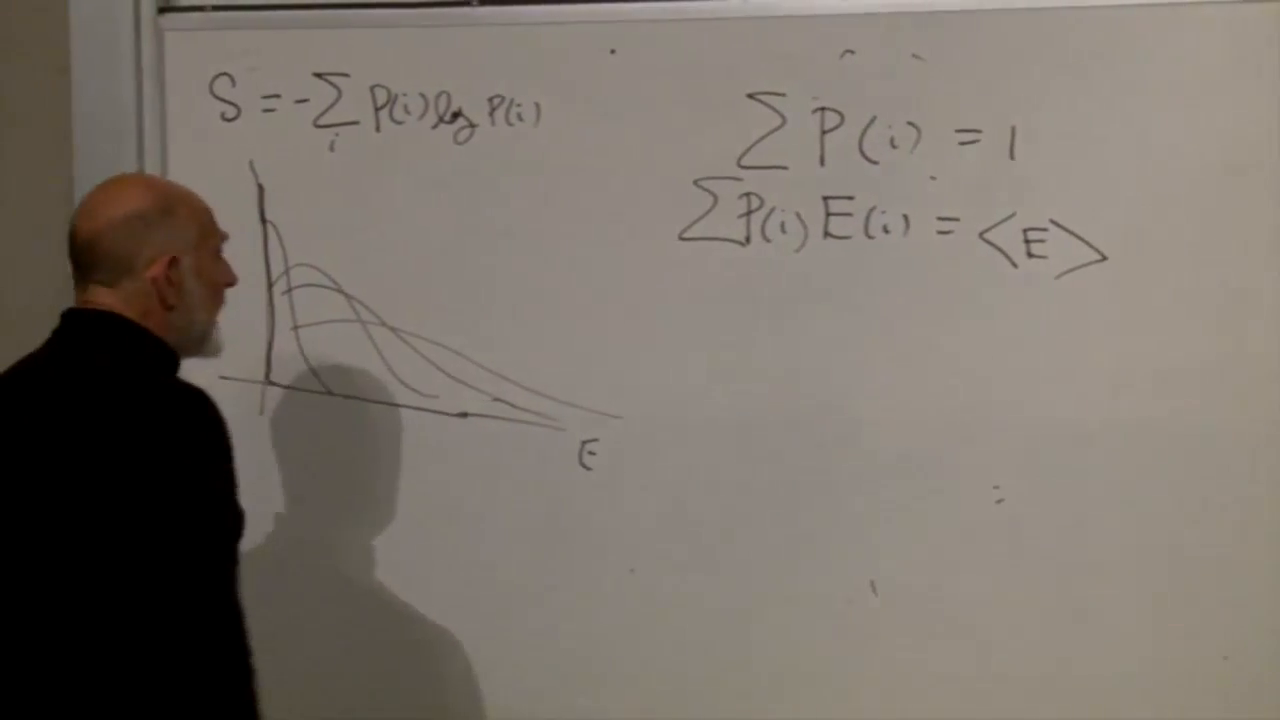
\includegraphics[width=0.88\textwidth]{lecture_03_figure_02.png}
\caption{На первой доске собраны формулы для энтропии, нормировки и средней энергии вместе с качественным семейством равновесных распределений.}
\lectureframe{00:06:44}
\end{figure}

\section{Равновесие как семейство распределений}

В предыдущей лекции у нас получилось однопараметрическое семейство равновесных распределений. Это семейство можно параметризовать температурой, но пока полезнее параметризовать его средней энергией \(\overline E\). При наименьшей возможной энергии распределение сосредоточено на основном состоянии:
\[
 P_i=\delta_{i0}.
\]
Тогда никакой неопределённости относительно состояния нет, и \(S=0\). По мере того как равновесное распределение распространяется на большее число энергетических уровней, растут и его средняя энергия, и его энтропия.

Это утверждение относится к тепловому семейству, а не ко всякому мыслимому распределению. Произвольное семейство могло бы смещаться к большим энергиям, одновременно сужаясь. Равновесные распределения, которые мы сейчас выведем, так себя не ведут в обычном режиме положительных температур. Вдоль этого семейства,
\begin{equation}
 \frac{dS}{d\overline E}>0.
 \label{eq:sm3-positive-temperature-branch}
\end{equation}
Системы с ограниченными спектрами могут также иметь ветви, на которых эта производная отрицательна. Такие режимы отрицательной температуры реальны, но в настоящем рассуждении мы их оставим в стороне.

Тепловое равновесие означает нечто большее, чем микроскопическую неподвижность. Молекулы продолжают двигаться, сталкиваться и обмениваться энергией. Стационарным стало макроскопическое описание: распределение больше не обнаруживает суммарного дрейфа, а отделённые части системы больше не поддерживают суммарный поток энергии.

\section{Законы термодинамики на языке статистики}

Первый закон — это закон сохранения энергии. Второй закон утверждает, что термодинамическая энтропия изолированной макроскопической системы не убывает:
\begin{equation}
 \Delta S_{\mathrm{tot}}\geq0.
 \label{eq:sm3-second-law}
\end{equation}
Равенство описывает равновесие или идеальное обратимое изменение; при спонтанной релаксации обычно имеет место строгое возрастание.

В вероятностной картине релаксация имеет тенденцию распределять вес по тем макроскопическим альтернативам, которые мы ещё различаем. Это утверждение требует оговорки, подчеркнутой на лекции: мы выполняем \emph{огрубление}. Точное гамильтоново развитие сохраняет тонкозернистую энтропию фазового пространства. Макроскопическая энтропия растёт потому, что мы перестаём отслеживать микроскопические корреляции и детали. Потеря такой информации расширяет редуцированное описание. Спонтанное сужение означало бы, напротив, что мы узнали микроскопическую информацию, не производя измерения.

Нулевой закон утверждает, что системы могут приходить к тепловому равновесию и что равновесие транзитивно. Если \(A\) находится в равновесии с \(B\), а \(B\) — с \(C\), то \(A\) находится в равновесии с \(C\). Температура задаёт величину, которая делает эту транзитивность наглядной:
\[
 T_A=T_B,\qquad T_B=T_C
 \quad\Longrightarrow\quad
 T_A=T_C.
\]
Вне равновесия энергия течёт от подсистемы с большей температурой к подсистеме с меньшей температурой. При равных температурах суммарный поток прекращается. Теперь мы выведем это операционное утверждение из энтропийного определения температуры.

\section{Почему энергия течёт от горячего к холодному}

Рассмотрим две слабо связанные подсистемы \(A\) и \(B\). Каждая из них находится во внутреннем равновесии, но их температуры различны. Выберем обозначения так, чтобы
\begin{equation}
 T_B>T_A>0.
 \label{eq:sm3-temperature-order}
\end{equation}
При малом обмене из сохранения полной энергии следует
\begin{equation}
 dE_A+dE_B=0.
 \label{eq:sm3-energy-conservation}
\end{equation}
Второй закон даёт
\begin{equation}
 dS_A+dS_B\geq0.
 \label{eq:sm3-entropy-change}
\end{equation}
Для каждой подсистемы, находящейся во внутреннем равновесии, температура определяется соотношением
\begin{equation}
 dE_X=T_X\,dS_X,
 \qquad X=A,B.
 \label{eq:sm3-temperature-differential}
\end{equation}
Подстановка в \eqref{eq:sm3-energy-conservation} даёт
\begin{equation}
 T_A\,dS_A+T_B\,dS_B=0,
\end{equation}
и, следовательно,
\begin{equation}
 dS_B=-\frac{T_A}{T_B}\,dS_A.
 \label{eq:sm3-dsb}
\end{equation}
Подставляя этот результат в \eqref{eq:sm3-entropy-change},
\begin{align}
 dS_{\mathrm{tot}}
 &=dS_A-\frac{T_A}{T_B}dS_A\\
 &=\frac{T_B-T_A}{T_B}\,dS_A\geq0.
 \label{eq:sm3-flow-entropy}
\end{align}
Поскольку \(T_B-T_A>0\) и \(T_B>0\), спонтанный обмен требует
\[
 dS_A>0.
\]
Тогда из \eqref{eq:sm3-temperature-differential} следует
\begin{equation}
 dE_A=T_A\,dS_A>0,
 \qquad
 dE_B=-dE_A<0.
 \label{eq:sm3-hot-to-cold}
\end{equation}
Энергия перетекла из \(B\), более горячей подсистемы, в \(A\), более холодную. Здесь теплота — это просто энергия в переносе. Поток продолжается до тех пор, пока не установится \(T_A=T_B\), когда изменение энтропии в первом порядке больше не благоприятствует ни одному направлению.

Тот же результат можно записать одной строкой:
\begin{equation}
 dS_{\mathrm{tot}}
 =dE_A\left(\frac{1}{T_A}-\frac{1}{T_B}\right)\geq0.
 \label{eq:sm3-compact-flow}
\end{equation}
Знак разности обратных температур определяет знак \(dE_A\). Эта компактная форма позднее естественно согласуется с каноническим ансамблем.

\begin{classroomqa}
\audiencequestion{Предполагает ли этот аргумент, что и \(A\), и \(B\) уже находятся во внутреннем равновесии?}
\lecturerresponse{Да. Приписывание одного \(T_A\) или \(T_B\) уже делает это предположение. Если подсистема не находится во внутреннем равновесии, разбейте её на меньшие области и применяйте этот аргумент локально везде, где можно определить температуру. Тогда глобальная релаксация складывается из обменов между этими областями.
\lecturetimestamp{00:24:38--00:25:22}}
\end{classroomqa}

\section{Что считать состоянием?}

Прежде чем искать равновесные вероятности, нужно понять, что означает метка \(i\). Микроскопическое состояние — это максимально полное описание системы, допускаемое лежащими в основе законами физики. В классической механике обычно мыслят положения и импульсы всех частиц. В квантовой механике состояние вместо этого представляет собой полное квантовое состояние; принцип неопределённости не позволяет одновременно точно задать все классические положения и импульсы.

Для квантовой системы в конечном ящике соответствующий счёт состояний может быть дискретным. Классическая статистическая механика возникает в подходящем пределе, где суммы по густо расположенным квантовым состояниям превращаются в интегралы по фазовому пространству. Этот предельный переход также вводит ячейку фазового пространства, необходимую для того, чтобы непрерывная энтропия была безразмерной; её нельзя получить простым заменением знака суммы на знак интеграла.

\begin{classroomqa}
\audiencequestion{Для газа следует ли представлять состояние как положения и импульсы каждой молекулы?}
\lecturerresponse{Это верная классическая картина. В более общем смысле состояние означает всё, что в принципе могло бы быть известно о системе, с учётом законов физики. Квантовая механика изменяет форму этого максимального описания и делает счёт при конечном объёме дискретным. Восстановление классического интеграла из квантовой суммы — это настоящий предельный переход, а не однострочная подстановка.
\lecturetimestamp{00:25:31--00:27:38}}
\end{classroomqa}

\section{Термостат из копий}

Теперь нельзя избежать трудного вопроса: после установления равновесия чем определяется \(P_i\)?

Поместим подсистему в контакт с очень большим термостатом. Энергия может переходить туда и обратно, но у термостата так много степеней свободы, что передача малого количества энергии почти не изменяет его температуру. Особенно удобный термостат состоит из многих слабо связанных копий самой подсистемы. Одна копия — это исследуемая система; остальные образуют её окружение.

Эта конструкция часто отражает реальную макроскопическую систему. Разделите большое почти однородное тело на много похожих ячеек. Каждая ячейка является подсистемой, а остальные ячейки служат для неё термостатом. Обозначим полное число копий через \(N\). В аудиторной демонстрации используются девять копий и три цветные метки состояний, но подсчёт не зависит от этих конкретных чисел.

Пусть \(n_i\) — число реплик в состоянии \(i\). Это \emph{числа заполнения}. Возможных энергетических уровней может быть бесконечно много, но при конечной полной энергии заполнение большинства очень высоких уровней пренебрежимо мало или равно нулю.

Первое ограничение — это просто число реплик:
\begin{equation}
 \sum_i n_i=N.
 \label{eq:sm3-number-constraint}
\end{equation}
Второе — полная энергия:
\begin{equation}
 \sum_i n_iE_i=N\overline E.
 \label{eq:sm3-total-energy-constraint}
\end{equation}
Правая часть экстенсивна. Если число реплик удвоить, удерживая их статистическое состояние фиксированным, полная энергия удваивается, тогда как средняя энергия на реплику остаётся \(\overline E\).

\begin{classroomqa}
\audiencequestion{Должно ли построение из реплик также удовлетворять энергетическому ограничению?}
\lecturerresponse{Да. Числа заполнения должны суммироваться в \(N\), а их взвешенная по энергии сумма должна равняться фиксированной полной энергии \(N\overline E\). Это как раз те два ограничения, которые позже будут наложены при максимизации энтропии.
\lecturetimestamp{00:37:12--00:39:54}}
\end{classroomqa}

Вероятность того, что случайно выбранная реплика находится в состоянии \(i\), равна её относительной частоте:
\begin{equation}
 P_i=\frac{n_i}{N},
 \qquad
 n_i=NP_i.
 \label{eq:sm3-frequency-probability}
\end{equation}

\begin{figure}[t]
\centering
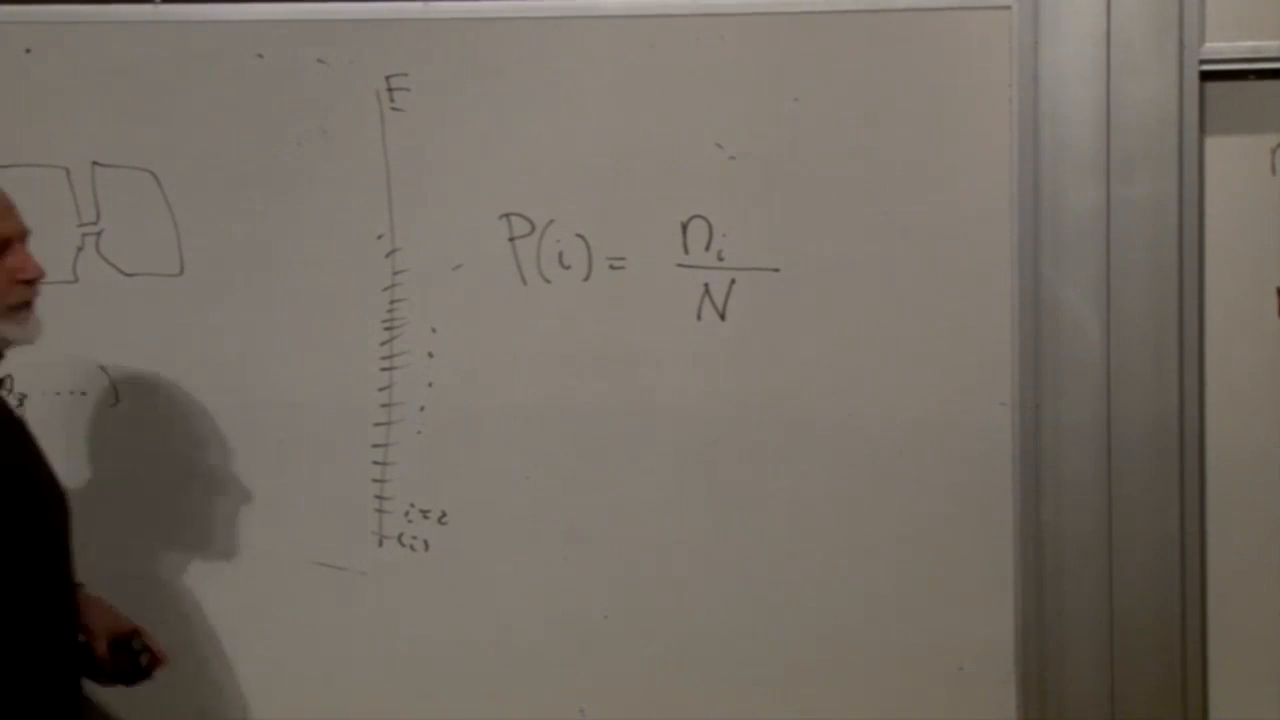
\includegraphics[width=0.82\textwidth]{lecture_03_figure_03.png}
\caption{Картина энергетических уровней и отождествление вероятности с долей заполнения \(P_i=n_i/N\).}
\lectureframe{00:41:40}
\end{figure}

\begin{classroomqa}
\audiencequestion{Означает ли запись \(N(i)\) на доске нечто отличное от \(n_i\)?}
\lecturerresponse{Нет. Оба обозначения означают число заполнения состояния \(i\). Мы последовательно используем \(n_i\), а прописную \(N\) оставляем для полного числа реплик.
\lecturetimestamp{00:41:28--00:41:33}}
\end{classroomqa}

Разделив \eqref{eq:sm3-number-constraint} и
\eqref{eq:sm3-total-energy-constraint} на \(N\), мы вновь получаем ограничения на вероятности:
\begin{equation}
 \sum_iP_i=1,
 \qquad
 \sum_iP_iE_i=\overline E.
 \label{eq:sm3-probability-constraints}
\end{equation}
Таким образом, частотная интерпретация ансамбля воспроизводит уравнения, с которых мы начали.

\section{Кратность схемы заполнения}

Зафиксируем набор чисел заполнения \(\{n_i\}\). Сколькими способами можно распределить \(N\) различимых реплик по состояниям так, чтобы реализовался в точности этот набор? Ответ даётся мультиномиальным коэффициентом
\begin{equation}
 C(\{n_i\})=\frac{N!}{\prod_i n_i!}.
 \label{eq:sm3-multiplicity}
\end{equation}
Чтобы понять знаменатель, сначала расположим все \(N\) помеченные реплики в \(N!\) порядках. Перестановка \(n_i\) реплик, занимающих одно и то же состояние, не даёт нового распределения реплик по состояниям, поэтому для каждого состояния нужно делить на \(n_i!\).

\begin{figure}[t]
\centering
\includegraphics[width=0.88\textwidth]{lecture_03_figure_04.png}
\caption{Мультиномиальная кратность
\(C=N!/\prod_i n_i!\), записанная на доске.}
\lectureframe{00:46:55}
\end{figure}

Незаполненные уровни не создают проблемы, поскольку \(0!=1\). Если все реплики занимают одно состояние, то
\[
 C=\frac{N!}{N!}=1,
\]
как и следует ожидать. Если три реплики занимают три различные заданные состояния, то
\[
 C=\frac{3!}{1!\,1!\,1!}=6.
\]
Если две реплики занимают два заданных состояния, формула даёт два распределения: можно поменять местами, какая помеченная реплика какое состояние занимает.

\begin{classroomqa}
\audiencequestion{Может ли более чем один набор чисел заполнения удовлетворять двум ограничениям?}
\lecturerresponse{Обычно таких наборов много. Уравнение
\eqref{eq:sm3-multiplicity} сначала подсчитывает число распределений для одного фиксированного набора
\(\{n_i\}\), ещё не решая, удовлетворяет ли он ограничениям. На следующем этапе сравниваются все наборы, совместимые с ограничениями, и находится тот, у которого кратность наибольшая.
\lecturetimestamp{00:48:07--00:48:43}}
\end{classroomqa}

Статистическое предположение состоит в том, что микроскопические распределения, совместимые с изолированными условиями, рассматриваются симметрично. Поэтому макроскопическая схема заполнения, реализуемая большим числом распределений, более вероятна. При больших
\(N\) распределение по долям \(n_i/N\) становится резко заострённым.
Равновесные доли — это значения, максимизирующие \(C\) при условиях
\eqref{eq:sm3-number-constraint} и
\eqref{eq:sm3-total-energy-constraint}.

\section{Приближение Стирлинга}

Факториалы становятся огромными задолго до того, как \(N\) достигает макроскопического значения, поэтому мы работаем с их логарифмами. Начнём с
\begin{equation}
 \log N!=\sum_{x=1}^{N}\log x.
 \label{eq:sm3-log-factorial-sum}
\end{equation}
Для больших \(N\) сумма приближается площадью под \(\log x\):
\begin{align}
 \log N!
 &\simeq\int_1^N\log x\,dx\\
 &=\left[x\log x-x\right]_1^N\\
 &=N\log N-N+1.
 \label{eq:sm3-stirling-integral}
\end{align}
Первообразная непосредственно следует из
\[
 \frac{d}{dx}(x\log x-x)=\log x.
\]
В ведущем экстенсивном порядке аддитивную константу можно отбросить:
\begin{equation}
 \log N!\simeq N\log N-N.
 \label{eq:sm3-stirling-log}
\end{equation}
Возведение в экспоненту даёт упрощённую форму, использованную в лекции,
\begin{equation}
 N!\simeq N^N e^{-N}.
 \label{eq:sm3-stirling-simple}
\end{equation}

\begin{figure}[t]
\centering
\includegraphics[width=0.88\textwidth]{lecture_03_figure_05.png}
\caption{Старшее приближение Стирлинга и его вывод заменой суммы \(\log x\) интегралом.}
\lectureframe{01:03:45}
\end{figure}

\begin{classroomqa}
\audiencequestion{Не остаётся ли при вычислении \(x\log x-x\) на нижнем пределе дополнительное \(+1\)?}
\lecturerresponse{Да. Уравнение \eqref{eq:sm3-stirling-integral} содержит эту константу. Она пренебрежимо мала по сравнению с членами, пропорциональными \(N\), при \(N\to\infty\), поэтому в ведущей формуле её опускают. Сама сумма должна начинаться с \(x=1\); \(\log0\) не определён.
\lecturetimestamp{01:04:12--01:04:35}}
\end{classroomqa}

\begin{classroomqa}
\audiencequestion{Не отсутствует ли также множитель, пропорциональный \(\sqrt{N}\)?}
\lecturerresponse{Да. Более точная асимптотическая формула имеет вид
\[
 N!\sim\sqrt{2\pi N}\left(\frac{N}{e}\right)^N.
\]
Её логарифм добавляет лишь \(\tfrac12\log(2\pi N)\), что субэкстенсивно по сравнению с \(N\log N-N\). Это важно для точных вероятностей при конечном \(N\), но не для ведущего расчёта энтропии макроскопической системы.
\lecturetimestamp{01:04:35--01:05:40}}
\end{classroomqa}

Приближение Стирлинга нужно также применять с осторожностью в знаменателе
\eqref{eq:sm3-multiplicity}. В термодинамическом пределе состояния с ненулевыми предельными вероятностями имеют \(n_i=NP_i\), так что их заполнения растут вместе с \(N\). Состояния с очень малым или исчезающим заполнением можно обработать, введя отсечение по конечной энергии, а затем восстановить предельным переходом. Ведущая экстенсивная энтропия не зависит от отброшенных подведущих членов.

\section{Логарифм кратности — это энтропия}

Применим \eqref{eq:sm3-stirling-simple} к числителю и ко всем макроскопически заполненным множителям в знаменателе:
\begin{equation}
 C\simeq
 \frac{N^Ne^{-N}}
 {\prod_i n_i^{\,n_i}e^{-n_i}}.
 \label{eq:sm3-c-stirling}
\end{equation}
Поскольку \(\sum_i n_i=N\), ведущие экспоненциальные множители сокращаются:
\begin{equation}
 C\simeq\frac{N^N}{\prod_i n_i^{\,n_i}}.
 \label{eq:sm3-c-leading}
\end{equation}
Максимизировать логарифм легче, чем произведение, а логарифм монотонен, поэтому оба максимума достигаются при одной и той же схеме заполнения:
\begin{equation}
 \log C=N\log N-\sum_i n_i\log n_i.
 \label{eq:sm3-logc-occupations}
\end{equation}
Теперь подставим \(n_i=NP_i\):
\begin{align}
 \log C
 &=N\log N-\sum_iNP_i\log(NP_i)\\
 &=N\log N-N\sum_iP_i\log N
   -N\sum_iP_i\log P_i\\
 &=-N\sum_iP_i\log P_i,
 \label{eq:sm3-logc-entropy-derivation}
\end{align}
где благодаря нормировке сокращаются два члена \(N\log N\). Следовательно, в ведущем порядке по \(N\),
\begin{equation}
 \boxed{\log C=NS}.
 \label{eq:sm3-logc-ns}
\end{equation}

\begin{figure}[t]
\centering
\includegraphics[width=0.88\textwidth]{lecture_03_figure_06.png}
\caption{Вычисление на доске, связывающее
\(\log C=N\log N-\sum_i n_i\log n_i\) с
\(-N\sum_iP_i\log P_i=NS\).}
\lectureframe{01:16:10}
\end{figure}

Это соотношение — идейный центр главы. Энтропия не является посторонней величиной, навязанной задаче подсчёта. Это логарифм кратности, отнесённый к одной реплике. Поэтому максимизация числа микроскопических распределений тождественна, в ведущем порядке, максимизации энтропии одной реплики.

\begin{classroomqa}
\audiencequestion{Разве кратность не была бы наибольшей, если бы все числа заполнения были равны?}
\lecturerresponse{Равномерное распределение получается, когда никакое состояние не выделено и на конечном наборе состояний наложено только
\(\sum_i n_i=N\). Ограничение фиксированной энергии меняет ответ, потому что значения \(E_i\) различны. Равные заполнения, вообще говоря, не дают заданной средней энергии.
\lecturetimestamp{01:17:07--01:18:20}}
\end{classroomqa}

\begin{classroomqa}
\audiencequestion{Величина \(N\) велика, но почему приближение Стирлинга можно применять к каждому \(n_i\) в знаменателе?}
\lecturerresponse{Для каждого состояния с ненулевой предельной вероятностью
\(n_i=NP_i\) растёт пропорционально \(N\). Можно сначала сохранить конечный энергетический диапазон, взять в нём предел при больших \(N\), а затем расширить этот диапазон. Разреженные хвостовые состояния требуют отдельных конечных поправок, но они не изменяют ведущую экстенсивную энтропию.
\lecturetimestamp{01:18:23--01:19:28}}
\end{classroomqa}

\begin{classroomqa}
\audiencequestion{Именно это приближение при больших \(N\) ранее имелось в виду под огрублением?}
\lecturerresponse{Нет. Термодинамический предел управляет большими числами заполнения и асимптотическим подсчётом. Огрубление — это потеря или намеренное отбрасывание микроскопического разрешения. Это разные операции, хотя обе часто используются в макроскопической статистической механике.
\lecturetimestamp{01:19:29--01:19:46}}
\end{classroomqa}

\begin{classroomqa}
\audiencequestion{Поскольку
\(\log C=N\log N-\sum_i n_i\log n_i\), не следует ли минимизировать второй член, а не максимизировать его?}
\lecturerresponse{Да; при фиксированном \(N\) максимизация \(\log C\) эквивалентна минимизации \(\sum_i n_i\log n_i\). После подстановки \(n_i=NP_i\) фиксированные члены \(N\log N\) сокращаются, и остаётся
\(-N\sum_iP_i\log P_i=NS\). Тем самым ту же самую операцию естественнее описывать как максимизацию положительной энтропии \(S\).
\lecturetimestamp{01:19:48--01:20:55}}
\end{classroomqa}

\begin{classroomqa}
\audiencequestion{Почему не завершить рассуждение сразу по соображениям симметрии и не положить все \(n_i\) равными?}
\lecturerresponse{Этот короткий путь игнорирует энергетические метки. Ограничение нормировки трактует состояния симметрично, но
\(\sum_iP_iE_i=\overline E\) этого не делает: состояния с разной энергией вносят разный вклад. Именно в энергетическом ограничении и появляется неравномерное равновесное распределение.
\lecturetimestamp{01:21:15--01:21:41}}
\end{classroomqa}

\section{Задача максимизации энтропии}

Теперь мы можем сформулировать статистико-механическое правило без двусмысленности. Варьируйте вероятности \(P_i\) и максимизируйте
\begin{equation}
 S[P]=-\sum_iP_i\log P_i
 \label{eq:sm3-maximize-entropy}
\end{equation}
при условиях
\begin{equation}
 \sum_iP_i=1,
 \qquad
 \sum_iP_iE_i=\overline E.
 \label{eq:sm3-maxent-constraints}
\end{equation}
Вероятности, при которых достигается максимум, задают резко предпочтительные доли заполнения в большом ансамбле реплик. Числа заполнения флуктуируют, но их относительные отклонения уменьшаются с ростом \(N\), так что отношения \(n_i/N\) становятся хорошо определёнными термодинамическими вероятностями.

\begin{classroomqa}
\audiencequestion{Являются ли \(E_i\) фиксированными энергиями состояний, тогда как в ограничении используется отдельно заданная полная энергия?}
\lecturerresponse{Да. Спектр \(\{E_i\}\) относится к подсистеме.
Полная совокупность реплик имеет фиксированную полную энергию, но энергия
непрерывно переходит между репликами. Деление этой полной энергии на \(N\) фиксирует среднюю
энергию \(\overline E\) одной реплики, а не её энергию в каждой микроскопической
реализации.
\lecturetimestamp{01:26:12--01:27:07}}
\end{classroomqa}

Задачу легко сформулировать, но она ещё не решена. Это задача на экстремум с двумя ограничениями, поэтому нужен ещё один математический инструмент.

\section{Множители Лагранжа}

Для функции \(F(x_1,x_2,\ldots)\) без ограничений стационарная точка
удовлетворяет
\begin{equation}
 \frac{\partial F}{\partial x_i}=0
 \qquad\text{for every }i.
 \label{eq:sm3-unconstrained-stationary}
\end{equation}
Теперь потребуем дополнительно, чтобы
\begin{equation}
 G(x_1,x_2,\ldots)=0.
 \label{eq:sm3-one-constraint}
\end{equation}

\begin{classroomqa}
\audiencequestion{Что означает \(x\), если на рисунке координатами служат \(x\)
и \(y\)?}
\lecturerresponse{Здесь \(x\) — сокращённое обозначение всего вектора координат
\((x_1,x_2,\ldots)\). На двумерном рисунке его компонентами являются
просто \(x\) и \(y\). Позже компонентами будут вероятности
\(P_1,P_2,\ldots\).
\lecturetimestamp{01:30:12--01:30:20}}
\end{classroomqa}

Геометрически линии уровня \(F=\text{constant}\) образуют контурную карту,
а \(G=0\) — кривую, по которой системе разрешено двигаться. Условный
экстремум возникает там, где одна из линий уровня \(F\) касается кривой
ограничения. В этой точке градиенты параллельны:
\begin{equation}
 \nabla F=-\lambda\nabla G
 \label{eq:sm3-parallel-gradients}
\end{equation}
для некоторого числа \(\lambda\).

\begin{figure}[t]
\centering
\includegraphics[width=0.88\textwidth]{lecture_03_figure_07.png}
\caption{Геометрия линий уровня на доске и дополненная функция
\(F'=F+\lambda G\). Условный экстремум возникает в точке касания.}
\lectureframe{01:37:10}
\end{figure}

Уравнение \eqref{eq:sm3-parallel-gradients} можно получить, определив
дополненную функцию
\begin{equation}
 F'=F+\lambda G
 \label{eq:sm3-augmented-function}
\end{equation}
и потребовав обычной стационарности:
\begin{equation}
 \frac{\partial F'}{\partial x_i}=0.
 \label{eq:sm3-augmented-stationarity}
\end{equation}
Множитель \(\lambda\) поначалу неизвестен. Из-за этого система не
остаётся недоопределённой, потому что исходное ограничение \(G=0\) даёт ещё
одно уравнение.

\begin{classroomqa}
\classquestion{Почему добавление члена, пропорционального \(G\), делает
стационарной точку, удовлетворяющую ограничению?}
\lecturerresponse{В условном экстремуме смещение по касательной к \(G=0\)
уже не даёт изменения \(F\) в первом порядке. Остаётся только наклон по
нормали к ограничению. Поскольку \(\nabla G\) направлен в ту же нормальную
сторону, подходящий \(\lambda\) его компенсирует:
\(\nabla F+\lambda\nabla G=0\).
\lecturetimestamp{01:35:06--01:35:32}}
\end{classroomqa}

\section{Пример с двумя переменными}

Требуется минимизировать
\begin{equation}
 F(x,y)=\frac{x^2+y^2}{2}
 \label{eq:sm3-example-f}
\end{equation}
при условии
\begin{equation}
 x+y=1.
 \label{eq:sm3-example-constraint}
\end{equation}
Запишем ограничение как \(G=x+y-1=0\) и составим
\begin{equation}
 F'=\frac{x^2+y^2}{2}+\lambda(x+y-1).
 \label{eq:sm3-example-augmented}
\end{equation}
Стационарные уравнения имеют вид
\begin{align}
 \frac{\partial F'}{\partial x}&=x+\lambda=0,\\
 \frac{\partial F'}{\partial y}&=y+\lambda=0.
 \label{eq:sm3-example-derivatives}
\end{align}
Следовательно, \(x=y=-\lambda\). Оставшееся уравнение — это ограничение,
\[
 x+y=-2\lambda=1,
\]
поэтому
\begin{equation}
 \lambda=-\frac12,
 \qquad
 x=y=\frac12.
 \label{eq:sm3-example-solution}
\end{equation}
Точка \((1/2,1/2)\) — это место, где наименьшая окружность с центром в начале
координат касается прямой \(x+y=1\).

\begin{figure}[t]
\centering
\includegraphics[width=0.88\textwidth]{lecture_03_figure_08.png}
\caption{Полное вычисление методом множителей Лагранжа для минимизации
\((x^2+y^2)/2\) при условии \(x+y=1\).}
\lectureframe{01:44:10}
\end{figure}

При нескольких ограничениях введите по одному множителю для каждого:
\begin{equation}
 F'=F+\lambda_1G_1+\lambda_2G_2+\cdots.
 \label{eq:sm3-many-multipliers}
\end{equation}
Затем решайте
\begin{equation}
 \begin{aligned}
 \frac{\partial F'}{\partial x_i}&=0
 &&\text{for every }i,\\
 G_a&=0
 &&\text{for every constraint }a.
 \end{aligned}
 \label{eq:sm3-many-equations}
\end{equation}
В лекции предлагается намеренно искусственная тренировочная задача: найти
экстремум квадратичной функции от \(x,y,z\) при наложении двух независимых
линейных ограничений, например \(x+y=1\) и \(z+x=1\). Её цель — не конкретный
ответ, а правило, что каждое ограничение вносит и один множитель, и одно
уравнение.

\section{Задача, подготовленная к следующей лекции}

В статистической механике координатами служат вероятности
\(\{P_i\}\), максимизируемой функцией является энтропия, а ограничениями
— нормировка и фиксированная средняя энергия. Определим
\begin{align}
 S[P]&=-\sum_iP_i\log P_i,\\
 G_1[P]&=\sum_iP_i-1,\\
 G_2[P]&=\sum_iP_iE_i-\overline E.
 \label{eq:sm3-final-functions}
\end{align}
Поэтому дополненную энтропию можно записать в виде
\begin{equation}
 \Phi[P]
 =S[P]+\alpha G_1[P]+\beta G_2[P].
 \label{eq:sm3-final-augmented}
\end{equation}
Уравнения, которые нужно решить, таковы:
\begin{equation}
 \frac{\partial\Phi}{\partial P_i}=0
 \quad\text{for every }i,
 \qquad
 G_1=0,
 \qquad
 G_2=0.
 \label{eq:sm3-final-problem}
\end{equation}

\begin{figure}[H]
\centering
\includegraphics[width=0.88\textwidth]{lecture_03_figure_09.png}
\caption{Заключительная запись на доске: энтропия как функция вероятностей
вместе с нормировкой и фиксированной средней энергией.}
\lectureframe{01:53:05}
\end{figure}

На этом этапе задача полностью поставлена. Решение
\eqref{eq:sm3-final-problem} даёт равновесное распределение. Множитель,
сопряжённый с энергией, станет обратной температурой
\(\beta=1/T\) с точностью до соглашения о знаке, выбранного в
\eqref{eq:sm3-final-augmented}. На следующей лекции выполняется это
дифференцирование и получаются больцмановские веса.

\chapter{Веса Больцмана, статистические суммы и идеальный газ}

\lectureoverview{Мы выводим равновесное распределение вероятностей, максимизируя энтропию при фиксированных нормировке и средней энергии. Затем статистическая сумма позволяет получить среднюю энергию, энтропию и температуру дифференцированием. Первым полным примером служит идеальный газ; затем следуют гравитационное обобщение и предварительный взгляд на флуктуации энергии.}

\section{Задача об энтропии при ограничениях}

Начнем с большой совокупности из \(\mathcal N\) одинаковых, очень слабо взаимодействующих реплик одной и той же подсистемы. Если \(n_i\) реплик находятся в \(i\)-м состоянии, то
\begin{equation}
 p_i=\frac{n_i}{\mathcal N},
 \qquad
 \sum_i p_i=1.
 \label{eq:sm4-occupation-probability}
\end{equation}
Мультиномиальный подсчет из предыдущей лекции дает энтропию на одну реплику,
\begin{equation}
 S[p]=-\sum_i p_i\log p_i.
 \label{eq:sm4-entropy}
\end{equation}
Полезно рассматривать ее как обычную функцию всех переменных \(p_1,p_2,\ldots\). Именно ее простая аддитивная форма делает вычисление возможным.

Совокупность реплик имеет фиксированную полную энергию \(\mathcal N E\), где \(E\) — средняя энергия на одну реплику. Поэтому второе ограничение имеет вид
\begin{equation}
 \sum_i p_iE_i=E.
 \label{eq:sm4-energy-constraint}
\end{equation}
Уровни \(E_i\) относятся к подсистеме; число \(E\) в правой части есть их среднее, взвешенное вероятностями. Максимизация
\eqref{eq:sm4-entropy}
при ограничениях
\eqref{eq:sm4-occupation-probability} и
\eqref{eq:sm4-energy-constraint} выбирает доли заселения, которые с подавляющим превосходством наиболее вероятны.

Для удобства будем минимизировать \(-S=\sum_i p_i\log p_i\). Введем по одному множителю Лагранжа для каждого ограничения:
\begin{equation}
 \begin{aligned}
 \Phi[p;\alpha,\beta]
 &=\sum_i p_i\log p_i\\
 &\quad+\alpha\left(\sum_i p_i-1\right)\\
 &\quad+\beta\left(\sum_i p_iE_i-E\right).
 \end{aligned}
 \label{eq:sm4-augmented-functional}
\end{equation}
Символы \(\alpha\) и \(\beta\) пока не выражают никаких физических предположений. На этом этапе это просто два числа, необходимые для наложения двух ограничений.

\begin{classroomqa}
\audiencequestion{Является ли дополненная функция также функцией \(\alpha\) и \(\beta\)?}
\lecturerresponse{Да. Варьирование по \(\alpha\) и \(\beta\) восстанавливает два ограничения. Однако в непосредственном вычислении мы держим эти множители фиксированными и варьируем вероятности \(p_i\). Их значения затем определяются нормировкой и предписанной средней энергией.
\lecturetimestamp{00:09:32--00:09:49}}
\end{classroomqa}

\begin{figure}[t]
\centering
\includegraphics[width=0.92\textwidth]{lecture_04_figure_02.png}
\caption{Дополненный функционал энтропии после опускания членов, постоянных при вариации вероятностей.}
\lectureframe{00:10:56}
\end{figure}

При дифференцировании по вероятности члены
\(-\alpha\) и \(-\beta E\) не дают вклада. Именно этот сокращенный функционал виден на доске. Они остаются частью
\eqref{eq:sm4-augmented-functional}; для данной производной они просто стали несущественными.

\section{Распределение Больцмана}

Выберем любую одну вероятность. В лекции выбрано \(p_7\), отчасти потому, что \(1\) выглядит слишком особенным, а \(7\) — счастливое число. От этого выбора ничто не зависит. Все нужное дифференцирование сводится к
\begin{equation}
 \frac{d}{dp_i}\bigl(p_i\log p_i\bigr)=\log p_i+1.
\end{equation}
Поэтому
\begin{equation}
 \frac{\partial\Phi}{\partial p_i}
 =\log p_i+1+\alpha+\beta E_i=0.
 \label{eq:sm4-stationarity}
\end{equation}
Решая относительно \(p_i\),
\begin{align}
 \log p_i&=-(1+\alpha)-\beta E_i,\\
 p_i&=e^{-(1+\alpha)}e^{-\beta E_i}.
\end{align}
Первый множитель не зависит от метки состояния. Обозначим его через \(1/Z\):
\begin{equation}
 p_i=\frac{e^{-\beta E_i}}{Z}.
 \label{eq:sm4-boltzmann-weight}
\end{equation}

Вот первый неожиданный результат. Стандартное дифференцирование с ограничениями привело к экспоненциальному закону. Относительные вероятности подчиняются соотношению
\begin{equation}
 \frac{p_i}{p_j}=e^{-\beta(E_i-E_j)}.
 \label{eq:sm4-relative-weight}
\end{equation}
Множитель \(\beta\) управляет тем, насколько быстро вероятность убывает с ростом энергии. Большие положительные \(\beta\) концентрируют распределение около самых низких уровней; малые положительные \(\beta\) оставляют заметный вес и на более высоких уровнях спектра. Мы уже видим, что изменение \(\beta\) меняет среднюю энергию, хотя его отождествление с обратной температурой еще предстоит доказать.

\section{Нормировка и статистическая сумма}

Нормировка определяет не зависящий от состояния множитель:
\begin{equation}
 1=\sum_i p_i
 =\frac{1}{Z}\sum_i e^{-\beta E_i},
\end{equation}
поэтому
\begin{equation}
 Z(\beta)=\sum_i e^{-\beta E_i}.
 \label{eq:sm4-partition-function}
\end{equation}
Это каноническая статистическая сумма. Сначала она появилась как нормировочная константа, но такое описание сильно преуменьшает ее роль. Как только \(Z(\beta)\) известна, термодинамические величины получаются из ее производных.

Уровни энергии в \eqref{eq:sm4-partition-function} являются исходными данными. Они следуют из механики системы вместе с фиксированными внешними условиями: объемом и формой ящика, магнитными или электрическими полями и любыми другими управляющими параметрами. Изменение управляющего параметра меняет спектр и, следовательно, меняет \(Z\). В настоящем вычислении эти параметры, а значит и набор \(\{E_i\}\), считаются фиксированными.

\begin{classroomqa}
\audiencequestion{Что именно представляют оси на экспоненциальном эскизе? Вертикальная координата — это какое-то одно конкретное \(p_i\)?}
\lecturerresponse{Изображенная высота — это вероятность, приписанная уровню, тогда как горизонтальный порядок можно читать либо как метку состояния
\(i\), либо, что физически содержательнее, как энергию \(E_i\). Каждому состоянию соответствует фиксированная энергия. Большие \(\beta\) заставляют вероятность круто убывать с этой энергией; вблизи \(\beta=0\) веса почти постоянны на доступных уровнях.
\lecturetimestamp{00:19:39--00:20:09}}
\end{classroomqa}

\section{Средняя энергия, скрытая в статистической сумме}

Второе ограничение определяет \(\beta\):
\begin{equation}
 E=\sum_i p_iE_i
 =\frac{1}{Z}\sum_i E_i e^{-\beta E_i}.
 \label{eq:sm4-mean-energy}
\end{equation}
Вместо того чтобы заново вычислять эту взвешенную сумму, продифференцируем
\eqref{eq:sm4-partition-function}:
\begin{equation}
 \frac{dZ}{d\beta}
 =-\sum_i E_i e^{-\beta E_i}.
\end{equation}
Сравнение с \eqref{eq:sm4-mean-energy} дает
\begin{equation}
 E(\beta)
 =-\frac{1}{Z}\frac{dZ}{d\beta}
 =-\frac{d\log Z}{d\beta}.
 \label{eq:sm4-energy-logz}
\end{equation}
Логарифм здесь естественен, потому что его производная дает множитель
\(1/Z\).

\begin{figure}[t]
\centering
\includegraphics[width=0.82\textwidth]{lecture_04_figure_03.png}
\caption{На доске одновременно записаны нормировка, ограничение на среднюю энергию и производная статистической суммы.}
\lectureframe{00:26:24}
\end{figure}

\begin{classroomqa}
\audiencequestion{Нижнее уравнение на доске — это новое уравнение для \(Z\) или оно получается из определения над ним?}
\lecturerresponse{Оно получается дифференцированием определения
\(Z=\sum_i e^{-\beta E_i}\). При взятии производной появляется множитель
\(-E_i\). Деление результата на \(Z\) затем воспроизводит взвешенную сумму, определяющую среднюю энергию.
\lecturetimestamp{00:25:58--00:26:37}}
\end{classroomqa}

\begin{classroomqa}
\audiencequestion{Делает ли
\(dZ/d\beta=-E Z\) функцию \(Z\) собственной функцией операции дифференцирования?}
\lecturerresponse{Не в обычном смысле. В уравнении на собственные значения \(Z\) умножалась бы на постоянную, тогда как здесь
\(E=E(\beta)\). Это уравнение задает среднюю энергию как функцию \(\beta\); это не задача на фиксированное собственное значение.
\lecturetimestamp{00:28:49--00:29:43}}
\end{classroomqa}

Простота \eqref{eq:sm4-energy-logz} обманчива. Спектр может быть сложным, и вычисление \(Z\) может оказаться трудным, но как только эта единственная функция найдена, средняя энергия получается одной производной. Такой мотив повторяется по всей статистической механике: элементарные операции, примененные в правильном порядке, дают результаты, которые было бы трудно напрямую угадать.

\begin{classroomqa}
\audiencequestion{\(E\) — это полная энергия всех реплик или средняя энергия одного ящика?}
\lecturerresponse{Это средняя энергия одного ящика. Совокупность реплик имеет полную энергию \(\mathcal N E\). Позже, когда в качестве системы будет выбран целый ящик, содержащий \(N\) частиц газа, \(E\) будет означать энергию всего этого образца газа.
\lecturetimestamp{00:30:55--00:31:10}}
\end{classroomqa}

\begin{classroomqa}
\audiencequestion{Можно ли брать логарифм от
\(\sum_i e^{-\beta E_i}\) почленно?}
\lecturerresponse{Нет. Логарифм превращает произведение в сумму, но не сумму в сумму логарифмов:
\[
 \log\!\left(\sum_i e^{-\beta E_i}\right)
 \ne \sum_i\log\!\left(e^{-\beta E_i}\right).
\]
Это различие пригодится позже, когда у независимых подсистем статистические суммы перемножаются.
\lecturetimestamp{00:31:10--00:31:58}}
\end{classroomqa}

\section{Что фиксировано и чему позволено меняться?}

В одних и тех же формулах присутствуют несколько уровней переменных, и в обсуждении на занятии они намеренно разграничиваются.

\begin{itemize}
 \item Вероятности \(p_i\) — это исходные неизвестные.
 \item Уровни \(E_i\) фиксированы, как только заданы система и ее управляющие параметры.
 \item Множитель \(\alpha\) поглощен нормировкой
 \(Z=e^{1+\alpha}\).
 \item Для предписанной средней энергии \(E\) ограничение фиксирует одно число
 \(\beta\). Однако в семействе равновесных состояний можно использовать либо
 \(E=E(\beta)\), либо \(\beta=\beta(E)\).
\end{itemize}

\begin{classroomqa}
\audiencequestion{Если множители — числа, почему \(\beta\) и
\(E\) теперь рассматриваются как переменные?}
\lecturerresponse{Для одной задачи с ограничениями это действительно числа. Но мы можем сравнивать много равновесных задач с одним и тем же спектром и разными предписанными средними энергиями. В таком семействе \(\beta\) меняется с
\(E\). Фиксация \(E\) определяет \(\beta\); фиксация \(\beta\) определяет
\(E\). Это два способа читать одно и то же соотношение.
\lecturetimestamp{00:31:58--00:33:27}}
\end{classroomqa}

\begin{classroomqa}
\audiencequestion{Исчезло ли \(\alpha\)?}
\lecturerresponse{Исчезло только его имя. Определение
\(e^{-(1+\alpha)}=1/Z\) поглощает его в \(Z\). Сохранять одновременно и \(\alpha\),
и \(Z\) значило бы дважды учитывать один и тот же параметр нормировки.
\lecturetimestamp{00:33:29--00:33:49}}
\end{classroomqa}

Энергия не обязана быть единственной сохраняющейся величиной. Если ограничены полный импульс, число частиц, момент импульса или какая-либо другая величина, ее среднему значению соответствует собственный множитель. Такое расширение меняет ансамбль, но не метод.

\begin{classroomqa}
\audiencequestion{Не делаем ли мы, фиксируя только среднюю энергию, слишком сильных предположений о системе?}
\lecturerresponse{Это предполагает, что в данной задаче не нужно накладывать условие ни на какую другую сохраняющуюся величину. Если, например, фиксирован и полный импульс, нужно добавить ещё одно ограничение и ещё один множитель Лагранжа. Напротив, объём, форма и внешние поля здесь являются управляющими параметрами: они считаются фиксированными и сами определяют энергетические уровни.
\lecturetimestamp{00:33:51--00:35:50}}
\end{classroomqa}

\begin{classroomqa}
\audiencequestion{Должна ли \(\alpha\) фигурировать как ещё один аргумент энергии, и зависит ли \(Z\) от уровней \(E_i\)?}
\lecturerresponse{\(\alpha\) уже содержится в \(Z\), так что независимым аргументом она не является. Статистическая сумма, разумеется, зависит как от фиксированного спектра, так и от \(\beta\). Изменение управляющего параметра изменяет \(E_i\) и, следовательно, изменяет \(Z\); при нынешних производных по \(\beta\) спектр считается фиксированным.
\lecturetimestamp{00:35:52--00:37:10}}
\end{classroomqa}

\begin{classroomqa}
\audiencequestion{Варьируем ли мы отдельные уровни \(E_i\) или среднюю энергию \(E\)?}
\lecturerresponse{Отдельные уровни остаются фиксированными. Средняя энергия меняется потому, что меняются вероятности. Таким образом, семейство параметризуется \(E\) или, эквивалентно, \(\beta\), тогда как один и тот же список уровней \(\{E_i\}\) используется повсюду.
\lecturetimestamp{00:37:12--00:39:04}}
\end{classroomqa}

На практике температуру часто гораздо легче измерить, чем полную энергию газа. Мы можем поместить термометр; взвешивать релятивистскую разность масс и ссылаться на \(E=mc^2\) было бы корректно, но поразительно бесполезно. Чтобы придать \(\beta\) операциональный смысл, нужно теперь связать его с термодинамическим определением температуры.

\section{Энтропия раньше температуры}

Логически энтропия предшествует температуре. Подставим вероятности Больцмана в \eqref{eq:sm4-entropy}:
\begin{equation}
 \log p_i=-\beta E_i-\log Z.
\end{equation}
Тогда
\begin{align}
 S
 &=-\sum_i p_i\log p_i\\
 &=\beta\sum_i p_iE_i+\log Z\sum_i p_i\\
 &=\beta E+\log Z.
 \label{eq:sm4-entropy-logz}
\end{align}
Сумма нормировки даёт конечный множитель, равный единице. Это также первый намёк на свободную энергию Гельмгольца, поскольку позже \(F_{\mathrm H}=-T\log Z\) в единицах, где \(k_B=1\).

\begin{classroomqa}
\audiencequestion{Что случилось с множителем \(1/Z\) в первом члене?}
\lecturerresponse{Он уже входит в \(p_i\). Сумма \(\sum_i p_iE_i\) включает полную нормированную вероятность и по определению является средней энергией \(E\).
\lecturetimestamp{00:43:19--00:43:26}}
\end{classroomqa}

\begin{classroomqa}
\audiencequestion{Не должен ли в \(S=\beta E+\log Z\) стоять минус?}
\lecturerresponse{Нет. Энтропия начинается с минуса, а \(\log p_i=-\beta E_i-\log Z\) содержит ещё два минуса. В итоге они дают два положительных члена, выписанных в \eqref{eq:sm4-entropy-logz}.
\lecturetimestamp{00:45:53--00:46:03}}
\end{classroomqa}

Температура была термодинамически определена как
\begin{equation}
 dE=T\,dS,
 \qquad
 \frac{1}{T}=\frac{dS}{dE},
 \label{eq:sm4-temperature-definition}
\end{equation}
при всех остальных фиксированных управляющих параметрах. Первая попытка продифференцировать \eqref{eq:sm4-entropy-logz} непосредственно по \(E\) быстро загромождается, потому что \(\beta\) тоже зависит от \(E\). Чище взять полный дифференциал:
\begin{align}
 dS
 &=\beta\,dE+E\,d\beta
   +\frac{d\log Z}{d\beta}\,d\beta\\
 &=\beta\,dE+E\,d\beta-E\,d\beta\\
 &=\beta\,dE.
 \label{eq:sm4-entropy-differential}
\end{align}
Сокращение использует \eqref{eq:sm4-energy-logz}. Сравнение \eqref{eq:sm4-entropy-differential} с \eqref{eq:sm4-temperature-definition} даёт
\begin{equation}
 T=\frac{1}{\beta},
 \qquad
 \beta=\frac{1}{T}.
 \label{eq:sm4-beta-temperature}
\end{equation}

\begin{figure}[t]
\centering
\includegraphics[width=0.82\textwidth]{lecture_04_figure_04.png}
\caption{Два члена с \(d\beta\) сокращаются, и остаётся \(dS=\beta\,dE\).}
\lectureframe{00:50:48}
\end{figure}

\begin{classroomqa}
\audiencequestion{Не предполагает ли это сокращение ошибочно, что \(\log Z\) не зависит от энергии или температуры?}
\lecturerresponse{Нет. При фиксированном спектре имеется один независимый термический параметр. Можно написать \(Z=Z(\beta)\), а затем рассматривать \(\beta=\beta(E)\) вдоль равновесного семейства. Полный дифференциал сохраняет всю зависимость от \(d\beta\), и тождество \(d\log Z/d\beta=-E\) как раз и обеспечивает это сокращение.
\lecturetimestamp{00:52:04--00:52:44}}
\end{classroomqa}

На протяжении большей части вычисления температура измеряется в единицах энергии, так что \(k_B=1\). Возвращаясь к лабораторным единицам,
\begin{equation}
 \beta=\frac{1}{k_B T_{\mathrm K}},
 \label{eq:sm4-beta-laboratory}
\end{equation}
где \(T_{\mathrm K}\) — абсолютная температура в кельвинах. Часто удобно писать \(T_{\mathrm e}=k_BT_{\mathrm K}\) и затем использовать \(\beta=1/T_{\mathrm e}\).

\begin{classroomqa}
\audiencequestion{Для некоторого объёма газа система — это одна молекула или вся совокупность?}
\lecturerresponse{Это зависит от того, как определена система. Здесь системой будет весь ящик с газом, так что \(E\) — это энергия всех его молекул. Для достаточно разреженного идеального газа одну молекулу тоже можно рассматривать как подсистему, поскольку частицы не взаимодействуют; факторизация ниже покажет связь между этими двумя описаниями.
\lecturetimestamp{00:53:32--00:54:49}}
\end{classroomqa}

Теперь можно собрать канонические тождества:
\begin{align}
 p_i&=\frac{e^{-\beta E_i}}{Z},&
 Z(\beta)&=\sum_i e^{-\beta E_i},\label{eq:sm4-canonical-pair}\\
 E&=-\frac{d\log Z}{d\beta},&
 S&=\beta E+\log Z,&
 T&=\frac{1}{\beta}.
 \label{eq:sm4-canonical-identities}
\end{align}

\section{Классический идеальный газ}

Рассмотрим \(N\) тождественных точечных частиц массы \(m\) в ящике объёма \(V\). Газ является идеальным, когда взаимодействиями между частицами можно пренебречь. Это может быть хорошим приближением либо потому, что силы слабы, либо потому, что газ настолько разрежен, что тесные сближения редки.

Классическое микросостояние задаётся всеми координатами и импульсами:
\begin{equation}
 (\bm q_1,\ldots,\bm q_N;\bm p_1,\ldots,\bm p_N).
\end{equation}
Имеется \(3N\) координат положения и \(3N\) координат импульса, поэтому состояние — это точка в фазовом пространстве размерности \(6N\). При отсутствии взаимодействий гамильтониан имеет вид
\begin{equation}
 H(\bm p)=\sum_{a=1}^{N}\frac{\bm p_a^2}{2m}
 =\sum_{\mu=1}^{3N}\frac{p_\mu^2}{2m}.
 \label{eq:sm4-ideal-hamiltonian}
\end{equation}

\begin{classroomqa}
\audiencequestion{Имеется ли \(3N\) частиц, и не приводит ли суммирование по всем компонентам импульса к двойному счёту состояний?}
\lecturerresponse{Частиц здесь \(N\), а компонент импульса — \(3N\). Сумма в \eqref{eq:sm4-ideal-hamiltonian} содержит по одному квадратичному члену для каждой компоненты. Затем интеграл по фазовому пространству интегрирует каждую независимую компоненту ровно один раз, так что из-за этого произведения двойного счёта не возникает.
\lecturetimestamp{01:02:29--01:04:04}}
\end{classroomqa}

Для непрерывного классического фазового пространства сумма по состояниям принимает вид
\begin{equation}
 Z_N
 =\frac{1}{N!\,h^{3N}}
 \int_{V^N}d^{3N}q
 \int_{\mathbb R^{3N}}d^{3N}p\,
 e^{-\beta H(\bm p)}.
 \label{eq:sm4-classical-partition}
\end{equation}
В лекции внимание сосредоточено на интегралах, и то же выражение записывается без ячейки фазового пространства \(h^{3N}\). Возвращение этого множителя делает \(Z_N\) безразмерной величиной и отражает квантовое происхождение классического подсчёта состояний. Поскольку \(h\) не зависит от \(\beta\), на производную, используемую ниже для вычисления энергии, он не влияет.

Интеграл по координатам берётся сразу. Гамильтониан не зависит от положения, и каждая частица может находиться где угодно в ящике:
\begin{equation}
 \int_{V^N}d^{3N}q=V^N.
\end{equation}
Интеграл по импульсам факторизуется в \(3N\) одинаковых одномерных гауссовых интегралов:
\begin{equation}
 Z_N
 =\frac{V^N}{N!\,h^{3N}}
 \left[
  \int_{-\infty}^{\infty}dp\,
  e^{-\beta p^2/(2m)}
 \right]^{3N}.
 \label{eq:sm4-factorized-gas}
\end{equation}

Множитель \(1/N!\) отождествляет конфигурации, различающиеся только перестановкой тождественных частиц. Для средней энергии при фиксированных \(N\) и \(V\) он даёт лишь не зависящую от \(\beta\) константу в \(\log Z_N\), поэтому исчезает под действием \(-\partial/\partial\beta\). Однако далеко не во всяком вопросе им можно пренебречь: вместе с \(h^{3N}\) он необходим для безразмерной статистической суммы, экстенсивной энтропии и согласованного химического потенциала.

Теперь положим
\begin{equation}
 x=\sqrt{\frac{\beta}{2m}}\,p,
 \qquad
 dp=\sqrt{\frac{2m}{\beta}}\,dx.
\end{equation}
Тогда гауссов интеграл принимает вид
\begin{align}
 \int_{-\infty}^{\infty}dp\,e^{-\beta p^2/(2m)}
 &=
 \sqrt{\frac{2m}{\beta}}
 \int_{-\infty}^{\infty}dx\,e^{-x^2}\\
 &=\sqrt{\frac{2\pi m}{\beta}}.
 \label{eq:sm4-gaussian}
\end{align}

\begin{figure}[t]
\centering
\includegraphics[width=0.82\textwidth]{lecture_04_figure_05.png}
\caption{Интеграл по импульсу сводится к стандартному гауссову интегралу одним масштабированием.}
\lectureframe{01:13:12}
\end{figure}

Подстановка в \eqref{eq:sm4-factorized-gas} даёт
\begin{equation}
 Z_N
 =\frac{V^N}{N!\,h^{3N}}
 \left(\frac{2\pi m}{\beta}\right)^{3N/2}.
 \label{eq:sm4-ideal-partition}
\end{equation}

\begin{figure}[t]
\centering
\includegraphics[width=0.78\textwidth]{lecture_04_figure_06.png}
\caption{На доске — окончательный вид статистической суммы идеального газа. Ячейка фазового пространства \(h^{3N}\) восстановлена в \eqref{eq:sm4-ideal-partition}.}
\lectureframe{01:14:38}
\end{figure}

Удобно записать тот же результат через тепловую длину волны де Бройля
\begin{equation}
 \lambda_T=\frac{h}{\sqrt{2\pi mT}}
 \qquad (k_B=1).
\end{equation}
Тогда
\begin{equation}
 Z_N=\frac{1}{N!}\left(\frac{V}{\lambda_T^3}\right)^N.
 \label{eq:sm4-thermal-wavelength-form}
\end{equation}

При макроскопических \(N\) формула Стирлинга даёт
\begin{equation}
 N!\simeq N^Ne^{-N}\sqrt{2\pi N}.
\end{equation}
Если сохранить только ведущую экспоненциальную зависимость и ввести \(\rho=N/V\),
\begin{equation}
 \frac{V^N}{N!}
 \simeq
 \frac{1}{\sqrt{2\pi N}}
 \left(\frac{e}{\rho}\right)^N.
 \label{eq:sm4-density-rewrite}
\end{equation}
Это аккуратная перегруппировка по плотности, сделанная в лекции. Множитель с квадратным корнем даёт подведущий вклад в \(\log Z_N\), но здесь он выписан, а не молча отброшен.

\begin{classroomqa}
\audiencequestion{Если \(1/N!\) не зависит от \(\beta\), значит ли это, что он вообще ни на что не влияет?}
\lecturerresponse{Для текущей производной средней энергии при фиксированных \(N\) и \(V\) он роли не играет, потому что добавляет не зависящую от \(\beta\) константу к \(\log Z_N\). Для абсолютной энтропии и для изменений числа частиц он важен. Не следует смешивать это ограниченное утверждение о производной с более широким утверждением о подсчёте состояний.
\lecturetimestamp{01:27:01--01:27:51}}
\end{classroomqa}

\section{Энергия и равнораспределение}

Произведения неудобно дифференцировать; логарифмы превращают их в суммы. Из \eqref{eq:sm4-ideal-partition} получаем
\begin{equation}
 \log Z_N
 =-\frac{3N}{2}\log\beta+\text{\(\beta\)-independent terms}.
 \label{eq:sm4-log-ideal-partition}
\end{equation}
Следовательно,
\begin{equation}
 E
 =-\frac{\partial\log Z_N}{\partial\beta}
 =\frac{3N}{2\beta}
 =\frac{3N}{2}T.
 \label{eq:sm4-ideal-energy}
\end{equation}
Энергия на частицу равна
\begin{equation}
 \frac{E}{N}=\frac{3}{2}T
 \qquad (k_B=1),
\end{equation}
или, в лабораторных единицах,
\begin{equation}
 \frac{E}{N}=\frac{3}{2}k_BT_{\mathrm K}.
 \label{eq:sm4-ideal-energy-lab}
\end{equation}

\begin{figure}[t]
\centering
\includegraphics[width=0.84\textwidth]{lecture_04_figure_07.png}
\caption{В энергию идеального газа вносит вклад только член \(-3N\log\beta/2\), что даёт \(E/N=3T/2\).}
\lectureframe{01:25:28}
\end{figure}

\begin{classroomqa}
\audiencequestion{Где в формулу для энергии входит постоянная Больцмана?}
\lecturerresponse{У теоретика температура \(T\) имеет размерность энергии. Чтобы пользоваться кельвинами, замените её на \(k_BT_{\mathrm K}\), получая \(E/N=3k_BT_{\mathrm K}/2\). Малое значение \(k_B\) переводит макроскопическое по величине численное значение температуры в микроскопический энергетический масштаб одной молекулы.
\lecturetimestamp{01:24:58--01:26:01}}
\end{classroomqa}

Число 3 возникает из трёх направлений пространства. Множитель 1/2 возникает из корневой зависимости каждого гауссова интеграла от \(1/\beta\). Каждая независимая квадратичная координата импульса даёт вклад \begin{equation}
 \frac{1}{2}T
\end{equation} в среднюю энергию. В \(d\) пространственных измерениях тот же довод даёт \(E/N=dT/2\). Это первое появление теоремы о равнораспределении.

Расчёт энтропии, заданный в конце лекции, следует из \(S=\beta E+\log Z_N\). Используя приближение Стирлинга,
\begin{equation}
 \frac{S}{N}
 \simeq
 \log\!\left[
  \frac{V}{N}
  \left(\frac{2\pi mT}{h^2}\right)^{3/2}
 \right]
 +\frac{5}{2},
 \label{eq:sm4-sackur-tetrode}
\end{equation}
с точностью до подведущей поправки при конечном \(N\). Восстановление \(k_B\) умножает правую часть на \(k_B\) и заменяет \(T\) на \(k_BT_{\mathrm K}\). Результат ясно показывает, почему нормировочные множители, которые выпали из выражения для энергии, необходимы для энтропии.

\section{Газ в гравитационном поле}

Вопрос о том, что будет, если поставить ящик на нейтронную звезду, подводит к гравитационному обобщению. Прежде чем переходить к нейтронной звезде, рассмотрим однородное поле \(g\) в обычной комнате. Выберем \(y=0\) на дне ящика с площадью основания \(A\) и высотой \(L\). Гамильтониан принимает вид
\begin{equation}
 H=\sum_{a=1}^{N}
 \left(\frac{\bm p_a^2}{2m}+mgy_a\right).
 \label{eq:sm4-gravity-hamiltonian}
\end{equation}
Интегралы по горизонтальным координатам по-прежнему дают \(A^N\), тогда как каждая вертикальная координата даёт вклад
\begin{equation}
 I_y(L)
 =\int_0^Ldy\,e^{-\beta mgy}
 =\frac{1-e^{-\beta mgL}}{\beta mg}.
 \label{eq:sm4-finite-height-integral}
\end{equation}

\begin{classroomqa}
\audiencequestion{Должен ли вертикальный интеграл действительно простираться до бесконечности или только до верхней границы ящика?}
\lecturerresponse{Для конечного ящика он должен идти от \(0\) до его высоты \(L\), как в \eqref{eq:sm4-finite-height-integral}. Переход к бесконечному верхнему пределу — это последующее упрощение, моделирующее атмосферу над поверхностью, а не конечную комнату.
\lecturetimestamp{01:30:25--01:31:32}}
\end{classroomqa}

Поэтому полная статистическая сумма при конечной высоте равна
\begin{equation}
 Z_N(L)
 =
 \frac{1}{N!\,h^{3N}}
 \left[
  A\,
  \frac{1-e^{-\beta mgL}}{\beta mg}
  \left(\frac{2\pi m}{\beta}\right)^{3/2}
 \right]^N.
 \label{eq:sm4-gravity-partition-finite}
\end{equation}
Вертикальный множитель зависит от \(\beta\), так что он должен давать вклад в энергию. Действительно,
\begin{equation}
 \langle U\rangle
 =N\left[
  \frac{1}{\beta}
  -\frac{mgL}{e^{\beta mgL}-1}
 \right].
 \label{eq:sm4-finite-gravity-energy}
\end{equation}
Этим завершается небольшой фрагмент интегрирования, который на лекции сначала оставляют как досадное вычисление.

Для атмосферы бесконечной высоты, \(L\to\infty\), и
\begin{equation}
 I_y(\infty)=\frac{1}{\beta mg}.
\end{equation}
Статистическая сумма принимает вид
\begin{equation}
 Z_N^{(\infty)}
 =
 \frac{1}{N!\,h^{3N}}
 \left[
  \frac{A}{\beta mg}
  \left(\frac{2\pi m}{\beta}\right)^{3/2}
 \right]^N.
 \label{eq:sm4-gravity-partition-infinite}
\end{equation}
Её логарифм, зависящий от \(\beta\), равен
\begin{equation}
 \log Z_N^{(\infty)}
 =-\frac{3N}{2}\log\beta-N\log\beta+\mathrm{const}.
\end{equation}
Первый член даёт кинетическую энергию \(3NT/2\); второй даёт среднюю гравитационную потенциальную энергию \(NT\). Следовательно,
\begin{equation}
 E_{\mathrm{tot}}=\frac{5N}{2}T
\end{equation}
для этой идеализированной неограниченной сверху атмосферы.

\begin{figure}[t]
\centering
\includegraphics[width=0.83\textwidth]{lecture_04_figure_08.png}
\caption{Статистическая сумма для бесконечной атмосферы добавляет \(-N\log\beta\) к \(\log Z\), что и является источником средней потенциальной энергии.}
\lectureframe{01:36:38}
\end{figure}

\begin{classroomqa}
\audiencequestion{Потребовало бы очень сильное гравитационное поле ещё одного множителя Лагранжа?}
\lecturerresponse{Нет, не просто потому, что поле сильное. Гравитация изменяет гамильтониан и тем самым энергетические уровни или вес в фазовом пространстве. Остаётся тот же энергетический множитель \(\beta\). Нейтронная звезда вносит дополнительные физические осложнения, но первой модификацией всё равно остаётся включение гравитационной потенциальной энергии в \(H\).
\lecturetimestamp{01:27:58--01:29:24}}
\end{classroomqa}

\section{Три вопроса в заключение}

\begin{classroomqa}
\audiencequestion{Какое уравнение задаёт распределение Больцмана и что оно утверждает о равновесии?}
\lecturerresponse{Распределение имеет вид
\[
 p_i=\frac{e^{-\beta E_i}}{Z}.
\]
Это распределение максимальной энтропии при условиях нормировки и фиксированной средней энергии. Среднюю энергию нужно вычислять по тем же вероятностям, а условие нормировки всё равно должно быть наложено, хотя в окончательной формуле оно выглядит почти автоматическим.
\lecturetimestamp{01:38:14--01:38:45}}
\end{classroomqa}

Эта процедура может казаться механической: записать статистическую сумму, взять логарифм и продифференцировать. И всё же получающиеся уравнения продолжают удивлять. Опыт подсказывает, какая простая операция должна следовать за какой, но от этого сама тема не становится менее занимательной.

\begin{classroomqa}
\audiencequestion{Можно ли применить эти идеи об энтропии к коллапсирующей звезде или чёрной дыре? Как энтропия может расти, если вещество занимает меньшую область?}
\lecturerresponse{Со звёздами трудно главным образом потому, что подробное описание их вещества сложно. Для чёрной дыры имеется более ясный эталон: её энтропия Бекенштейна--Хокинга является предельной гравитационной энтропией при заданных макроскопических ограничениях. Коллапс может увеличивать энтропию, пока не будет достигнуто это значение для чёрной дыры; для её дальнейшего увеличения нужно изменить доступную энергию или размер.
\lecturetimestamp{01:39:29--01:40:36}}
\end{classroomqa}

\begin{classroomqa}
\audiencequestion{Может ли статистическая сумма также вычислять флуктуации энергии?}
\lecturerresponse{Да. Одна производная даёт среднюю энергию, а вторая производная — её дисперсию:
\begin{align*}
 \frac{\partial^2\log Z}{\partial\beta^2}
 &=\langle E^2\rangle-\langle E\rangle^2\\
 &=\operatorname{Var}(E).
\end{align*}
В энергетических единицах это связано с теплоёмкостью соотношением \(\operatorname{Var}(E)=T^2C_V\). В лабораторных единицах — \(\operatorname{Var}(E)=k_BT_{\mathrm K}^2C_V\). Это соотношение для флуктуаций и будет следующим вычислением.
\lecturetimestamp{01:40:37--01:41:53}}
\end{classroomqa}

Флуктуации отличают статистическую механику от чисто непрерывного термодинамического описания. Их систематическое изучение, связанное прежде всего с Гиббсом и Эйнштейном, выявляет конечные микроскопические составляющие, стоящие за гладкими макроскопическими законами. Именно с этого начинается следующая лекция.
\chapter{Давление, свободная энергия и флуктуации энергии}

\lectureoverview{Мы выводим давление из статистической суммы, не предполагая кинетической картины ударов молекул о стенку. Геометрическая лемма преобразует адиабатическую производную в производные при фиксированной температуре, свободная энергия Гельмгольца дает связь с \(\log Z\), а первым приложением оказывается закон идеального газа. Затем мы используем ту же статистическую сумму, чтобы вывести равновесную флуктуацию энергии и ее связь с теплоемкостью.}

\section{Пусть математика проверит интуицию}

У термодинамики своеобразная репутация. Ее дифференциальное исчисление элементарно, однако выбор того, что дифференцировать и что держать фиксированным, может быть удивительно тонким. Наша задача намеренно узка: вычислить давление идеального газа. Однако путь к этому ответу должен быть достаточно общим и для систем, в которых привычная молекулярная картина уже не заслуживает доверия.

Кинетическую историю рассказать легко. Молекулы ударяются о стенку и меняют знак нормальной компоненты своего импульса. Импульс, переданный за единицу времени, дает силу, а сила на единицу площади дает давление. Мы уже знаем, что средняя кинетическая энергия одной молекулы в трех измерениях равна
\begin{equation}
 \left\langle \frac{p^2}{2m}\right\rangle=\frac{3}{2}T
 \qquad (k_B=1).
 \label{eq:sm5-mean-kinetic-energy}
\end{equation}
При изотропном распределении скоростей можно оценить частоту столкновений, перенос импульса в каждом столкновении и возникающее давление.

Но сама стенка, по-видимому, нарушает изотропию. Почему у молекул очень близко к границе должно быть то же распределение по модулям скоростей и направлениям, что и у молекул глубоко в объеме? В равновесии это так с точностью, существенной здесь, но такой вывод должен следовать из статистической механики, а не незаметно вноситься в расчет в виде интуиции. Столкновения между молекулами делают кинетический аргумент еще менее прозрачным. Невзаимодействующий газ прост именно потому, что это необычно простая система.

В физике бывают случаи, когда самый безопасный прием — временно отказаться от наглядной картины и положиться на математику. Сначала выделяют искомую величину, затем преобразуют общие соотношения и ждут, пока не появится узнаваемая формула. В конце интуиция возвращается, но тогда математика проверяет интуицию, а не наоборот. Удовольствие термодинамики состоит в удивительных соотношениях, которые возникают из этой процедуры.

Искомое соотношение — это уравнение состояния,
\begin{equation}
 P=P(T,V,N),
 \label{eq:sm5-equation-of-state-target}
\end{equation}
где \(N\) — количество вещества, \(T\) — температура, а \(V\) — объем. Удовлетворительный вывод должен по-прежнему иметь смысл, когда частицы взаимодействуют, или когда вещество является жидкостью, плазмой или твердым телом. Только окончательное вычисление статистической суммы будет специфично для идеального газа.

\section{Энтропия и свободная энергия Гельмгольца}

Для начала напомним канонические формулы, которые понадобятся позже. Для микросостояний, помеченных \(i\),
\begin{equation}
 \begin{aligned}
 S&=-\sum_i p_i\log p_i,\\
 p_i&=\frac{e^{-\beta E_i}}{Z},\\
 Z&=\sum_i e^{-\beta E_i}.
 \end{aligned}
 \label{eq:sm5-canonical-definitions}
\end{equation}
Логарифм вероятности равен
\begin{equation}
 \log p_i=-\beta E_i-\log Z.
 \label{eq:sm5-log-probability}
\end{equation}
Подстановка в выражение для энтропии дает
\begin{align}
 S
 &=-\sum_i p_i\log p_i \notag\\
 &=\beta\sum_i p_iE_i+\log Z\sum_i p_i \notag\\
 &=\beta E+\log Z.
 \label{eq:sm5-entropy-log-z}
\end{align}
Здесь \(E=\sum_i p_iE_i\) — средняя энергия.

\begin{classroomqa}
\audiencequestion{Почему второй член дает только \(\log Z\), а не число состояний, умноженное на \(\log Z\)?}
\lecturerresponse{Суммируемый коэффициент — \(p_i\), а не \(1\). Нормировка дает \(\sum_i p_i=1\). Эквивалентно, числитель \(\sum_i e^{-\beta E_i}=Z\) сокращает \(Z\) в знаменателе. Число состояний на этом шаге вообще не появляется.
\lecturetimestamp{00:14:25--00:14:55}}
\end{classroomqa}

В энергетических единицах, используемых на большей части лекции, \(\beta=1/T\). Умножая \eqref{eq:sm5-entropy-log-z} на \(T\) и перегруппировывая члены, получаем
\begin{equation}
 E-TS=-T\log Z.
 \label{eq:sm5-helmholtz-identity}
\end{equation}
Комбинация в левой части встречается настолько часто, что заслуживает отдельного имени:
\begin{equation}
 A\equiv E-TS,
 \qquad
 A=-T\log Z.
 \label{eq:sm5-helmholtz-definition}
\end{equation}
Это свободная энергия Гельмгольца. Сейчас важнее не название, а само тождество; оно понадобится нам, когда давление будет преобразовано в производную статистической суммы.

\begin{figure}[t]
\centering
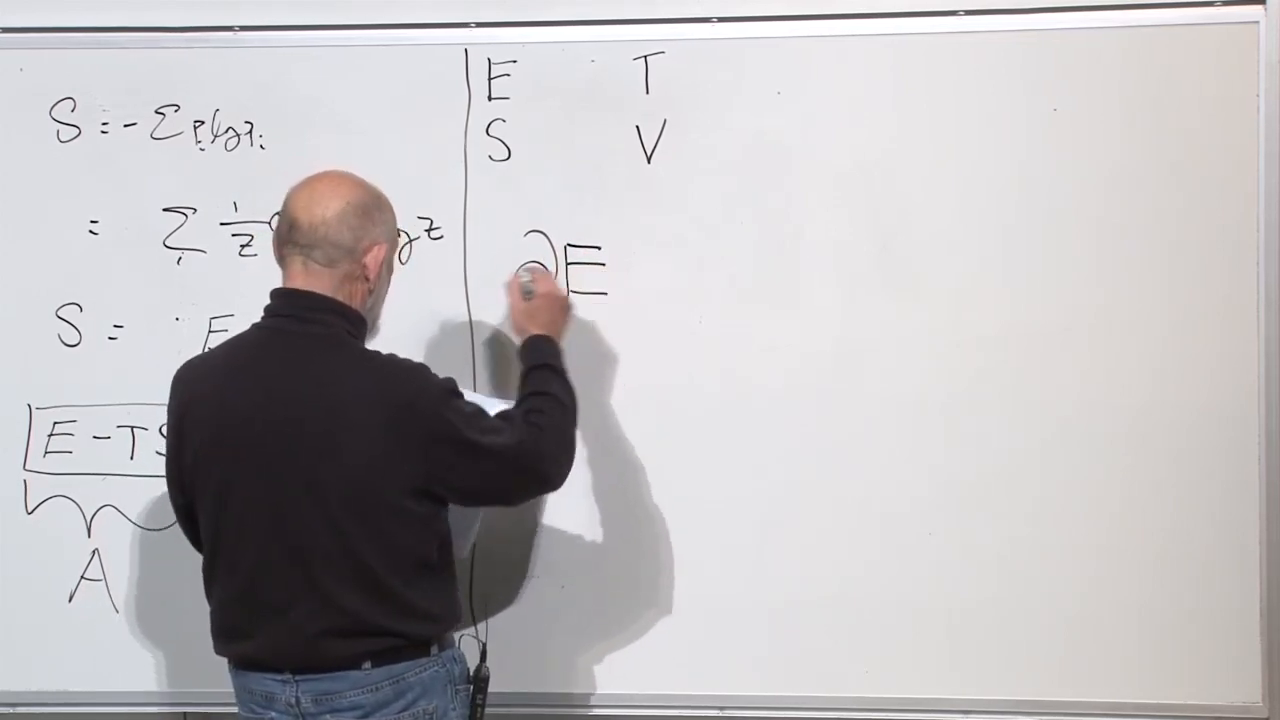
\includegraphics[width=0.90\textwidth]{lecture_05_figure_03.png}
\caption{Каноническое соотношение для энтропии, переписанное в виде \(A=E-TS=-T\log Z\).}
\lectureframe{00:16:50}
\end{figure}

\section{Управляющие параметры и их отклики}

Управляющий параметр — это макроскопическая величина, которую экспериментатор может изменять извне. Перемещая поршень, мы меняем объем, не манипулируя отдельными молекулами. Другими примерами служат приложенные электрические и магнитные поля. В более общем ансамбле можно также допустить изменение числа частиц.

Термодинамические переменные естественным образом образуют сопряженные пары. В данной задаче управляющим параметром является объем, а откликом на него — давление. Мы изменяем \(V\); давление показывает, как система энергетически сопротивляется этому изменению. Позже производная энергии сделает эту сопряженность точной.

\begin{classroomqa}
\audiencequestion{Можно ли само давление рассматривать как управляющий параметр?}
\lecturerresponse{Можно поставить эксперимент, в котором фиксируется внешнее давление, но в используемой здесь постановке положение поршня фиксирует объем, а внутреннее давление является откликом. Давление и объем — сопряженные переменные; какая из этих величин управляется, зависит от ансамбля и экспериментальной установки.
\lecturetimestamp{00:19:22--00:20:01}}
\end{classroomqa}

\begin{classroomqa}
\audiencequestion{Предполагается ли, что все молекулы одинаковы, или рассуждение ограничено газом?}
\lecturerresponse{Нет, такое ограничение не требуется для термодинамического рассуждения. Цилиндр может содержать несколько видов частиц, жидкость или даже твердое тело, подвергаемое сжатию. Статистическая сумма идеального газа будет лишь частным применением после того, как установлена общая формула для давления.
\lecturetimestamp{00:20:02--00:20:39}}
\end{classroomqa}

\begin{classroomqa}
\audiencequestion{Можно ли изменять количество вещества как еще одно внешнее воздействие?}
\lecturerresponse{Да. Число частиц — еще один возможный управляющий параметр. Если рассматривать его как динамическую величину, возникает собственная сопряженная переменная — химический потенциал. Для сегодняшнего вычисления \(N\) остается фиксированным.
\lecturetimestamp{00:20:39--00:20:57}}
\end{classroomqa}

\begin{classroomqa}
\audiencequestion{Могут ли жидкая вода и водяной пар одновременно присутствовать в равновесии?}
\lecturerresponse{При температуре и давлении сосуществования — да. Гравитация может располагать жидкость ниже пара, и все же обе фазы могут иметь одну и ту же температуру и оставаться в тепловом равновесии. Применима та же общая статистико-механическая схема.
\lecturetimestamp{00:20:59--00:21:36}}
\end{classroomqa}

В следующем рассуждении рассматривайте энергию и энтропию как зависимые функции двух независимо регулируемых переменных:
\begin{equation}
 E=E(T,V),
 \qquad
 S=S(T,V).
 \label{eq:sm5-dependent-functions}
\end{equation}
Температура и объем задают координаты в термодинамическом пространстве состояний. Энергия и энтропия ставят в соответствие числа каждой равновесной точке этого пространства.

\section{Производная при постоянной энтропии}

Производная, которая нам в конечном счете нужна, необычна:
\[
 \left(\frac{\partial E}{\partial V}\right)_S.
\]
Хотя \(T\) и \(V\) являются независимыми координатами, эта производная требует изменять \(V\), одновременно накладывая условие, что зависимая функция \(S(T,V)\) остается постоянной. Это производная вдоль кривой на плоскости \((T,V)\), а не вдоль координатной оси.

\begin{classroomqa}
\audiencequestion{Как \(T\) и \(V\) могут быть независимыми, если позднее используется производная \(dT/dV\)?}
\lecturerresponse{Они независимы на всем пространстве состояний. Как только мы накладываем ограничение \(S(T,V)=\mathrm{constant}\), допустимые состояния лежат на одномерном контуре. Вдоль этого контура \(T\) становится функцией \(V\), и его наклон \(dT/dV\) определен однозначно.
\lecturetimestamp{01:01:18--01:02:09}}
\end{classroomqa}

\begin{lemma}
Если \(E(T,V)\) и \(S(T,V)\) дифференцируемы, то везде, где
\((\partial S/\partial T)_V\neq0\),
\begin{equation}
 \left(\frac{\partial E}{\partial V}\right)_S
 =
 \left(\frac{\partial E}{\partial V}\right)_T
 -
 \left(\frac{\partial E}{\partial S}\right)_V
 \left(\frac{\partial S}{\partial V}\right)_T.
 \label{eq:sm5-calculus-lemma}
\end{equation}
\end{lemma}

\begin{proof}
Для произвольного бесконечно малого смещения,
\begin{equation}
 dE=
 \left(\frac{\partial E}{\partial V}\right)_T dV
 +
 \left(\frac{\partial E}{\partial T}\right)_V dT.
 \label{eq:sm5-total-differential-e}
\end{equation}
При фиксированном \(V\) правило цепочки позволяет использовать \(S\) как промежуточную переменную:
\begin{equation}
 \left(\frac{\partial E}{\partial T}\right)_V
 =
 \left(\frac{\partial E}{\partial S}\right)_V
 \left(\frac{\partial S}{\partial T}\right)_V.
 \label{eq:sm5-chain-rule-e-s-t}
\end{equation}

Теперь ограничим смещение контуром, на котором \(S\) постоянно. Вдоль этого контура,
\begin{equation}
 0=dS=
 \left(\frac{\partial S}{\partial V}\right)_T dV
 +
 \left(\frac{\partial S}{\partial T}\right)_V dT.
 \label{eq:sm5-constant-entropy-differential}
\end{equation}
Решая относительно наклона контура, получаем
\begin{equation}
 \left(\frac{dT}{dV}\right)_S
 =
 -
 \frac{\left(\frac{\partial S}{\partial V}\right)_T}
 {\left(\frac{\partial S}{\partial T}\right)_V}.
 \label{eq:sm5-entropy-contour-slope}
\end{equation}
Разделим \eqref{eq:sm5-total-differential-e} на \(dV\), воспользуемся
\eqref{eq:sm5-chain-rule-e-s-t}
и подставим
\eqref{eq:sm5-entropy-contour-slope}:
\begin{align}
 \left(\frac{\partial E}{\partial V}\right)_S
 &=
 \left(\frac{\partial E}{\partial V}\right)_T
 +
 \left(\frac{\partial E}{\partial S}\right)_V
 \left(\frac{\partial S}{\partial T}\right)_V
 \left(\frac{dT}{dV}\right)_S \notag\\
 &=
 \left(\frac{\partial E}{\partial V}\right)_T
 -
 \left(\frac{\partial E}{\partial S}\right)_V
 \left(\frac{\partial S}{\partial V}\right)_T.
\end{align}
Множитель \((\partial S/\partial T)_V\) сократился, что и доказывает результат.
\end{proof}

\begin{figure}[t]
\centering
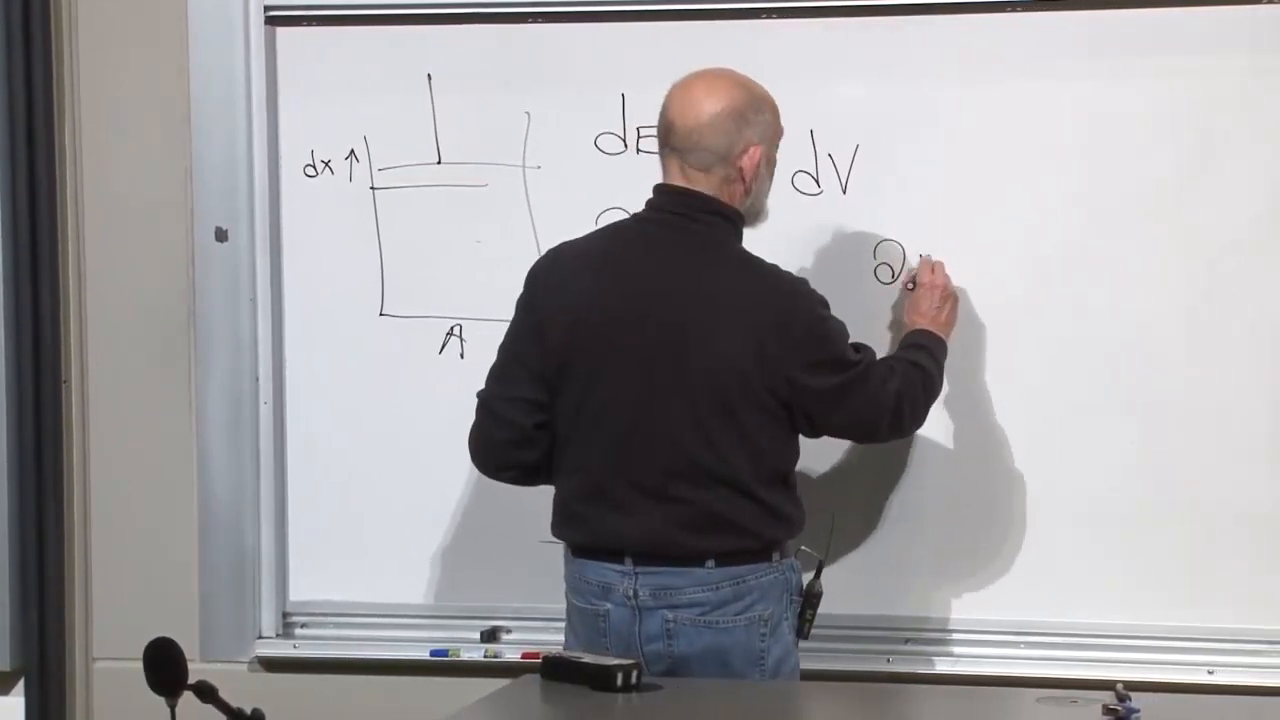
\includegraphics[width=0.90\textwidth]{lecture_05_figure_04.png}
\caption{Вычисление вдоль контура постоянной энтропии на этапе сокращения, завершающего лемму о производной.}
\lectureframe{00:36:10}
\end{figure}

Геометрическая картина здесь не просто украшение. Она объясняет, почему кажущаяся странной производная при фиксированном \(S\) может быть вычислена с помощью обычных частных производных по независимым координатам \(T\) и \(V\). Запись \(\delta E/\delta V\) в ходе построения служит полезным напоминанием о том, что эти символы представляют собой отношения малых изменений вдоль заданного пути.

\begin{classroomqa}
\audiencequestion{Является ли разложение \(dE\) просто обычным определением частных производных?}
\lecturerresponse{Да. В полном дифференциале ничего особенного не происходит. Единственная дополнительная деталь — последующее ограничение на контур \(dS=0\), которое определяет связь между \(dT\) и \(dV\).
\lecturetimestamp{00:29:26--00:29:32}}
\end{classroomqa}

\begin{classroomqa}
\audiencequestion{Требуется ли для сокращения, чтобы
\((\partial S/\partial T)_V\) была ненулевой?}
\lecturerresponse{Да. Для обычной устойчивой системы,
\[
 \left(\frac{\partial S}{\partial T}\right)_V
 =\frac{C_V}{T}>0,
\]

так что деление допустимо. Исключительные точки требуют отдельного рассмотрения.
При фиксированном гамильтониане повышение температуры расширяет каноническое распределение энергии и обычно увеличивает энтропию; понижение температуры сужает его. Именно таково физически правильное направление аргумента о монотонности.
\lecturetimestamp{00:36:50--00:37:47}}
\end{classroomqa}

\section{Работа поршня и адиабатическое условие}

Теперь придадим производной физический смысл. Рассмотрим поршень с
площадью поперечного сечения \(\mathcal A\). Если он смещается наружу на \(dx\), то
\begin{equation}
 dV=\mathcal A\,dx.
 \label{eq:sm5-piston-volume}
\end{equation}
Газ действует на поршень силой \(P\mathcal A\), поэтому работа,
совершаемая газом, равна
\begin{equation}
 \delta W_{\mathrm{by}}=P\mathcal A\,dx=P\,dV.
 \label{eq:sm5-piston-work}
\end{equation}
Если тепло в газ не поступает, то из закона сохранения энергии следует
\begin{equation}
 dE=-P\,dV.
 \label{eq:sm5-adiabatic-work}
\end{equation}
Знак имеет физический смысл: при расширении газ поднимает поршень или сообщает ему ускорение, а его собственная энергия уменьшается.

\begin{figure}[t]
\centering
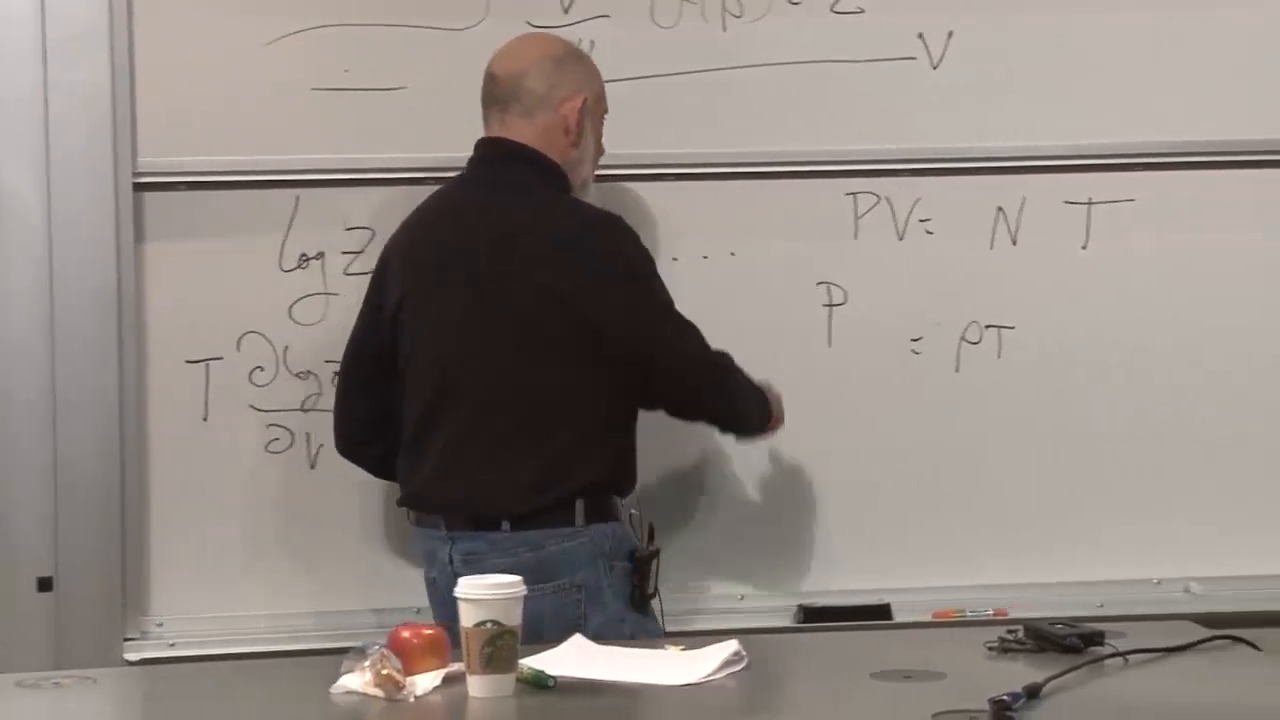
\includegraphics[width=0.90\textwidth]{lecture_05_figure_05.png}
\caption{Геометрия поршня и полученное соотношение для работы
\(dE=-P\,dV\).}
\lectureframe{00:43:10}
\end{figure}

Существенны две оговорки. Поршень должен двигаться достаточно медленно,
чтобы система оставалась сколь угодно близкой к равновесию, а стенки должны быть
теплоизолированы, чтобы энергия не подводилась в виде тепла. Быстрое вытягивание может быть настолько
стремительным, что за время движения ни одна молекула не достигнет удаляющегося поршня. Быстрое
сжатие порождает ударные волны. Ни один из этих процессов не представим
последовательностью равновесных состояний.

Термин \emph{адиабатический} иногда означает отсутствие теплообмена, а
иногда — медленное изменение. В обратимом процессе, который здесь требуется, присутствуют
обе идеи: изменение квазистатично и система теплоизолирована. При этих
условиях процесс также изоэнтропичен.

\begin{classroomqa}
\audiencequestion{Почему при адиабатическом изменении энтропия остается постоянной?}
\lecturerresponse{Рассмотрим систему с квантово-механической точки зрения. Ее многочастичные
энергетические уровни зависят от объема. Когда \(V\) медленно изменяется, адиабатическая
теорема непрерывно переводит каждый занятый уровень в его продолжение без
переходов между метками уровней. Энергии \(E_i(V)\) изменяются, но
вероятности заселения \(p_i\) остаются фиксированными. Поскольку
\(S=-\sum_i p_i\log p_i\) зависит от этих вероятностей, энтропия остается
постоянной. Теплообмен или необратимое движение сделали бы этот
вывод недействительным.
\lecturetimestamp{00:43:37--00:49:15}}
\end{classroomqa}

\begin{figure}[t]
\centering
\includegraphics[width=0.90\textwidth]{lecture_05_figure_06.png}
\caption{Многочастичные энергетические уровни, изменяющиеся с объемом, тогда как
вероятности их заселения сохраняют привязку к меткам уровней.}
\lectureframe{00:48:50}
\end{figure}

Уравнение \eqref{eq:sm5-adiabatic-work}, рассмотренное вдоль этого пути с постоянной
энтропией, задает давление в виде
\begin{equation}
 P=-\left(\frac{\partial E}{\partial V}\right)_S.
 \label{eq:sm5-pressure-fixed-entropy}
\end{equation}
Это сопряженное соотношение между давлением и объемом.

\begin{classroomqa}
\audiencequestion{Что происходит, если вместо этого перемещать поршень быстро?}
\lecturerresponse{Система выходит из равновесия, и детали ее динамики
становятся существенными. Внезапное сжатие порождает ударную волну.
При идеальном свободном расширении поршень может удалиться прежде, чем в него ударится хоть одна молекула, так что работа не совершается и
энергия остается постоянной, хотя объем меняется. Позднее газ
релаксирует к равновесию с возросшей энтропией. Такие процессы нельзя
описать единственной равновесной производной в
\eqref{eq:sm5-pressure-fixed-entropy}.
\lecturetimestamp{00:58:30--01:01:15}}
\end{classroomqa}

\begin{classroomqa}
\audiencequestion{Какое количественное условие определяет, является ли изменение
медленным?}
\lecturerresponse{Характерное время внешнего изменения должно быть велико по сравнению с
соответствующими внутренними временами релаксации. Для газа во время
макроскопического изменения должно происходить много молекулярных
столкновений и много ударов о стенки. Точный масштаб времени зависит от
вещества и геометрии, тогда как сам квазистатический предел является общим.
\lecturetimestamp{01:02:09--01:03:20}}
\end{classroomqa}

\section{От адиабатической энергии к статистической сумме}

Физическая формула \eqref{eq:sm5-pressure-fixed-entropy} пока еще не самая
удобная для вычисления. Каноническая статистическая механика естественным образом дает
функции температуры, потому что \(T\) непосредственно входит в больцмановский
вес. Лемма анализа переводит неудобную производную при фиксированной
энтропии в удобный для вычислений язык:
\begin{align}
 P
 &=
 -\left(\frac{\partial E}{\partial V}\right)_T
 +
 \left(\frac{\partial E}{\partial S}\right)_V
 \left(\frac{\partial S}{\partial V}\right)_T.
 \label{eq:sm5-pressure-lemma-substitution}
\end{align}
При фиксированном объеме первое начало дает \(dE=T\,dS\), и потому
\begin{equation}
 \left(\frac{\partial E}{\partial S}\right)_V=T.
 \label{eq:sm5-e-s-temperature}
\end{equation}
Следовательно
\begin{equation}
 P=
 -\left(\frac{\partial E}{\partial V}\right)_T
 +
 T\left(\frac{\partial S}{\partial V}\right)_T.
 \label{eq:sm5-pressure-fixed-temperature-pieces}
\end{equation}

\begin{classroomqa}
\audiencequestion{Откуда берется знак минус в формуле для давления?}
\lecturerresponse{Он возникает из работы, совершаемой газом:
\(dE=-P\,dV\) при адиабатическом расширении. В самой лемме анализа между ее
двумя членами стоит минус; общий минус в
\(P=-(\partial E/\partial V)_S\) меняет знак у них обоих, давая
\eqref{eq:sm5-pressure-fixed-temperature-pieces}.
\lecturetimestamp{00:52:40--00:53:14}}
\end{classroomqa}

Поскольку \(T\) фиксирована в обеих производных,
\begin{align}
 P
 &=
 -\left(\frac{\partial}{\partial V}(E-TS)\right)_T \notag\\
 &=
 -\left(\frac{\partial A}{\partial V}\right)_T.
 \label{eq:sm5-pressure-free-energy}
\end{align}
Наконец, подставим \(A=-T\log Z\):
\begin{equation}
 \boxed{
 P=
 T\left(\frac{\partial\log Z}{\partial V}\right)_T
 }.
 \label{eq:sm5-pressure-log-z}
\end{equation}

\begin{figure}[t]
\centering
\includegraphics[width=0.90\textwidth]{lecture_05_figure_07.png}
\caption{Сведение рассуждения при фиксированной температуре:
\(P=-(\partial A/\partial V)_T
=T(\partial\log Z/\partial V)_T\).}
\lectureframe{00:55:55}
\end{figure}

В \eqref{eq:sm5-pressure-log-z} нигде не предполагается идеальный газ. Если статистическую
сумму можно вычислить для взаимодействующей жидкости, плазмы или
твердого тела, то та же производная дает соответствующее давление. В более общем
виде каждому внешнему управляющему параметру соответствует сопряженный
отклик, получаемый дифференцированием подходящего термодинамического потенциала. В статистической
сумме закодированы многие такие отклики: дифференцирование \(\log Z\) по
\(\beta\) дает энергию, тогда как дифференцирование по
объему дает давление.

\section{Уравнение состояния идеального газа}

Лишь теперь перейдем к случаю \(N\) невзаимодействующих частиц. При сохранении классической
нормировки фазового пространства
\begin{equation}
 Z_N=
 \frac{1}{N!h^{3N}}
 \int d^{3N}q\,d^{3N}p\,
 \exp\!\left[
 -\beta\sum_{a=1}^{N}\frac{\mathbf p_a^2}{2m}
 \right].
 \label{eq:sm5-ideal-gas-partition-integral}
\end{equation}
Имеется \(3N\) координат положения и \(3N\) компонент импульса. Гамильтониан
не зависит от координат, поэтому каждая частица дает один множитель
объема сосуда:
\begin{equation}
 Z_N=
 \frac{V^N}{N!h^{3N}}I_p(\beta),
 \label{eq:sm5-ideal-gas-factorization}
\end{equation}
где весь интеграл по импульсам \(I_p(\beta)\) не зависит от \(V\).

\begin{classroomqa}
\audiencequestion{Почему здесь \(3N\) интегралов по координатам и \(3N\)
интегралов по импульсам?}
\lecturerresponse{Каждая из \(N\) частиц имеет три пространственные координаты
и три сопряженные компоненты импульса. Подсчет дает \(3N\) в каждой половине
фазового пространства, а не \(N\) частиц плюс еще \(3N\) частиц.
\lecturetimestamp{01:04:19--01:04:28}}
\end{classroomqa}

Логарифмирование отделяет зависимость от объема:
\begin{equation}
 \log Z_N
 =
 N\log V-\log N!-3N\log h+\log I_p(\beta).
 \label{eq:sm5-log-ideal-gas-partition}
\end{equation}
Множители \(1/N!\), \(h^{-3N}\) и \(I_p(\beta)\) все не зависят от
объема. Они важны для абсолютной энтропии и других вопросов, но не для
этой конкретной производной. Поэтому
\begin{equation}
 \left(\frac{\partial\log Z_N}{\partial V}\right)_T
 =\frac{N}{V}.
 \label{eq:sm5-log-z-volume-derivative}
\end{equation}
Уравнение \eqref{eq:sm5-pressure-log-z} сразу дает
\begin{equation}
 P=\frac{NT}{V},
 \qquad
 \boxed{PV=NT}.
 \label{eq:sm5-ideal-gas-law}
\end{equation}

\begin{classroomqa}
\audiencequestion{Означает ли \(N\) по-прежнему число реплик, использованных при выводе
распределения Больцмана?}
\lecturerresponse{Нет. Конструкция с репликами в предыдущем выводе была лишь счетным приемом и
здесь уже отсутствует. Здесь \(N\) — это число
реальных частиц в этом одном образце газа.
\lecturetimestamp{01:07:38--01:08:05}}
\end{classroomqa}

Введя численную плотность
\begin{equation}
 \rho=\frac{N}{V}
 \label{eq:sm5-number-density}
\end{equation}
получаем эквивалентную форму
\begin{equation}
 P=\rho T.
 \label{eq:sm5-density-equation-of-state}
\end{equation}

\begin{classroomqa}
\audiencequestion{Следует ли получать форму через плотность делением на \(N\)
или на \(V\)?}
\lecturerresponse{Разделите \(PV=NT\) на \(V\):
\(P=(N/V)T=\rho T\). Здесь \(\rho\) — численная плотность, а не массовая плотность.
\lecturetimestamp{01:08:45--01:09:16}}
\end{classroomqa}

\begin{figure}[t]
\centering
\includegraphics[width=0.90\textwidth]{lecture_05_figure_08.png}
\caption{Производная \(\log Z\) по объему и получающееся из нее уравнение состояния
идеального газа \(PV=NT\), или \(P=\rho T\).}
\lectureframe{01:09:25}
\end{figure}

Возвращаясь к лабораторной температуре \(T_K\),
\begin{equation}
 PV=Nk_BT_K.
 \label{eq:sm5-ideal-gas-law-laboratory}
\end{equation}
Этот знакомый результат согласуется с кинетической интуицией, но его вывод теперь
опирается на формализм, применимый далеко за пределами свободного газа.

\section{Второй выигрыш: равновесные флуктуации}

Вычисление давления завершено, но остается один обещанный вопрос:
что еще можно извлечь из статистической суммы? Рассмотрим систему,
находящуюся в тепловом контакте с термостатом. Ее энергия не фиксирована.
Энергия поступает и уходит, поэтому результаты повторных измерений флуктуируют вокруг канонического среднего.

\begin{classroomqa}
\audiencequestion{Можем ли мы теперь вычислить обещанные флуктуации?}
\lecturerresponse{Да. Оставшееся время позволяет еще раз продемонстрировать тот
же принцип: производные \(Z\) кодируют измеримую термодинамическую
информацию.
\lecturetimestamp{01:10:37--01:10:50}}
\end{classroomqa}

\subsection{Дисперсия и стандартное отклонение}

Для случайной величины \(x\) с \(\langle x\rangle=0\) мерой
ширины распределения служит \(\langle x^2\rangle\). Для общего распределения
сдвинем переменную на ее среднее:
\begin{equation}
 \delta x=x-\langle x\rangle.
 \label{eq:sm5-centered-variable}
\end{equation}
Ее среднее равно нулю,
\begin{equation}
 \langle\delta x\rangle
 =
 \langle x\rangle-\langle x\rangle=0,
 \label{eq:sm5-centered-mean}
\end{equation}
а ее средний квадрат равен
\begin{align}
 (\Delta x)^2
 &\equiv
 \left\langle\left(x-\langle x\rangle\right)^2\right\rangle \notag\\
 &=
 \langle x^2\rangle
 -2\langle x\rangle^2
 +\langle x\rangle^2 \notag\\
 &=
 \langle x^2\rangle-\langle x\rangle^2.
 \label{eq:sm5-variance}
\end{align}
Это и есть дисперсия. Ее положительный квадратный корень \(\Delta x\) — это стандартное
отклонение.

\begin{classroomqa}
\audiencequestion{Почему среднее от
\(x-\langle x\rangle\) в точности равно нулю?}
\lecturerresponse{Усреднение линейно, а \(\langle x\rangle\) уже является
числом. Поэтому
\(\langle x-\langle x\rangle\rangle
=\langle x\rangle-\langle x\rangle=0\).
\lecturetimestamp{01:14:02--01:14:22}}
\end{classroomqa}

\begin{classroomqa}
\audiencequestion{В чем различие между квадратом флуктуации, дисперсией, среднеквадратичной шириной и стандартным отклонением?}
\lecturerresponse{Дисперсия равна
\((\Delta x)^2=\langle x^2\rangle-\langle x\rangle^2\).
Стандартное отклонение — ее квадратный корень, \(\Delta x\). Для переменной с нулевым средним стандартное отклонение также является ее среднеквадратичным значением.
\lecturetimestamp{01:16:39--01:18:38}}
\end{classroomqa}

\begin{figure}[t]
\centering
\includegraphics[width=0.90\textwidth]{lecture_05_figure_09.png}
\caption{Сдвинутая переменная и разложение, приводящее к
\((\Delta x)^2=\langle x^2\rangle-\langle x\rangle^2\).}
\lectureframe{01:17:20}
\end{figure}

\subsection{Моменты энергии из статистической суммы}

Для канонического ансамбля,
\begin{align}
 \langle E\rangle
 &=
 \frac{1}{Z}\sum_i E_i e^{-\beta E_i} \notag\\
 &=
 -\frac{1}{Z}\frac{\partial Z}{\partial\beta}
 =
 -\frac{\partial\log Z}{\partial\beta}.
 \label{eq:sm5-mean-energy-from-z}
\end{align}
Одно дифференцирование по \(\beta\) со знаком минус дает умножение на один множитель \(E_i\). Вторая производная порождает \(E_i^2\):
\begin{equation}
 \langle E^2\rangle
 =
 \frac{1}{Z}\sum_i E_i^2e^{-\beta E_i}
 =
 \frac{1}{Z}\frac{\partial^2 Z}{\partial\beta^2}.
 \label{eq:sm5-second-energy-moment}
\end{equation}
Следовательно, дисперсия энергии равна
\begin{align}
 (\Delta E)^2
 &=
 \langle E^2\rangle-\langle E\rangle^2 \notag\\
 &=
 \frac{1}{Z}\frac{\partial^2Z}{\partial\beta^2}
 -
 \frac{1}{Z^2}
 \left(\frac{\partial Z}{\partial\beta}\right)^2 \notag\\
 &=
 \frac{\partial^2\log Z}{\partial\beta^2}
 =
 -\frac{\partial\langle E\rangle}{\partial\beta}.
 \label{eq:sm5-energy-variance-beta}
\end{align}
И снова на вид сложная наблюдаемая величина оказывается производной от
\(\log Z\).

\begin{figure}[t]
\centering
\includegraphics[width=0.90\textwidth]{lecture_05_figure_10.png}
\caption{Вторая производная \(\log Z\) по \(\beta\), отождествленная с дисперсией энергии.}
\lectureframe{01:29:00}
\end{figure}

\subsection{Теплоемкость и величина флуктуаций}

В используемых на лекции единицах \(T=1/\beta\), поэтому
\begin{equation}
 -\frac{\partial}{\partial\beta}
 =
 T^2\frac{\partial}{\partial T}.
 \label{eq:sm5-beta-temperature-derivative}
\end{equation}
При фиксированном объеме определим теплоемкость всего образца как
\begin{equation}
 C_V\equiv
 \left(\frac{\partial\langle E\rangle}{\partial T}\right)_V.
 \label{eq:sm5-heat-capacity}
\end{equation}
Уравнение \eqref{eq:sm5-energy-variance-beta} принимает вид
\begin{equation}
 \boxed{(\Delta E)^2=T^2C_V}
 \qquad (k_B=1).
 \label{eq:sm5-energy-fluctuation-lecture-units}
\end{equation}
Для лабораторной температуры \(T_K\), где
\(\beta=(k_BT_K)^{-1}\),
\begin{equation}
 \boxed{(\Delta E)^2=k_BT_K^2C_V}.
 \label{eq:sm5-energy-fluctuation-laboratory}
\end{equation}

\begin{figure}[t]
\centering
\includegraphics[width=0.90\textwidth]{lecture_05_figure_11.png}
\caption{Переход от производной по \(\beta\) к теплоемкости при фиксированном объеме, включая восстановленный множитель \(k_B\).}
\lectureframe{01:31:10}
\end{figure}

\begin{classroomqa}
\audiencequestion{Нужно ли в производной указывать фиксированный объем, а не фиксированное давление?}
\lecturerresponse{Да. В этом каноническом выводе внешние управляющие параметры гамильтониана, включая \(V\), удерживаются фиксированными. Получающаяся величина — \(C_V\). Ансамбль при постоянном давлении допускает флуктуации объема и работы и требует соответствующего термодинамического потенциала; нельзя просто заменить \(C_V\) на \(C_P\) в
\eqref{eq:sm5-energy-fluctuation-laboratory}.
\lecturetimestamp{01:29:01--01:29:28; 01:32:50--01:33:21}}
\end{classroomqa}

\begin{classroomqa}
\audiencequestion{Является ли \(C_V\) константой вещества?}
\lecturerresponse{Вообще говоря, нет. Она может зависеть от температуры, объема, фазы и состава. Кроме того, \(C_V\) здесь — теплоемкость всего образца и потому является экстенсивной величиной. Теплоемкость, отнесенную к массе, числу частиц или количеству вещества, получают только после деления на массу, число частиц или количество вещества.
\lecturetimestamp{01:31:47--01:32:21; 01:33:23--01:34:55}}
\end{classroomqa}

Для обычного экстенсивного вещества \(C_V\) пропорциональна \(N\), поэтому
\((\Delta E)^2\) пропорциональна \(N\), а \(\Delta E\) —
\(\sqrt{N}\). Сама средняя энергия пропорциональна \(N\). Следовательно,
\begin{equation}
 \frac{\Delta E}{\langle E\rangle}\sim\frac{1}{\sqrt{N}}.
 \label{eq:sm5-relative-fluctuation-scaling}
\end{equation}
Макроскопические относительные флуктуации ничтожны, тогда как в микроскопических образцах они проявляются непосредственно. Появление \(k_B\) в
\eqref{eq:sm5-energy-fluctuation-laboratory} указывает на эту связь между
термодинамическими наблюдаемыми и молекулярной дискретностью; или, что то же самое, оно связывает макроскопические единицы с подсчетом на авогадровском масштабе.

Давление и флуктуации теперь выводятся из одного и того же объекта:
\[
 P=T\left(\frac{\partial\log Z}{\partial V}\right)_T,
 \qquad
 (\Delta E)^2=\frac{\partial^2\log Z}{\partial\beta^2}.
\]
Это главный вывод. Как только правильно определены ограничения, статистическая сумма не просто нормирует вероятности. Ее производные задают измеримую термодинамику системы.

\chapter{Слабые взаимодействия, вириальные поправки и неполные дифференциалы}

\lectureoverview{Мы начинаем с операционального смысла измерения и температуры, а затем спрашиваем, как разреженный газ отклоняется от закона идеального газа, когда короткодействующие взаимодействия слабо включаются. Статистическая сумма дает первые поправки к энергии и давлению, обусловленные взаимодействием, и определяет область их применимости. В заключительном математическом отступлении функции состояния отличаются от теплоты и работы, зависящих от пути, с помощью полных дифференциалов, замкнутых контуров и конкретной проверки на идеальном газе.}

\section{Что на самом деле измеряет прибор}

Ни один лабораторный прибор не обращается к природе напрямую и не выдает абстрактную математическую переменную. Пружинный динамометр регистрирует удлинение; термометр — высоту столбика жидкости. Первое мы называем измерением силы, а второе — измерением температуры лишь потому, что между видимым откликом и искомой величиной установлено воспроизводимое соотношение.

Эта связь имеет ограниченную область применимости. Пружина подчиняется закону Гука лишь пока сохраняет упругость, а достаточно большая сила в конце концов деформирует ее или ломает. Более общо, если считываемая величина \(R\) гладко зависит от физической переменной \(X\), то вблизи выбранной рабочей точки \begin{equation}
 \Delta R \simeq
 \left.\frac{dR}{dX}\right|_{X_0}\Delta X.
 \label{eq:sm6-local-linear-response}
\end{equation} Малые изменения показания пропорциональны малым изменениям искомой переменной даже тогда, когда полная кривая отклика нелинейна. Такая локальная линеаризация и составляет обычную логику калибровки.

Показание может также зависеть от посторонних переменных. Пружина может слабо зависеть от температуры или давления. Высота ртутного столбика в термометре может зависеть от ориентации через действие тяжести, от свойств стекла или от медленных изменений материалов. Процедура измерения не доказывает, что этих зависимостей нет; она либо удерживает их фиксированными, либо показывает, что в требуемом масштабе ими можно пренебречь.

\begin{classroomqa} \audiencequestion{Могут ли локальное гравитационное поле или направление, в котором держат термометр, изменить показание?} \lecturerresponse{Да, в принципе. Если ориентация оказывает заметное влияние, то указание держать термометр вертикально становится частью определения прибора. У поверхности Земли гравитационное поле достаточно стабильно, поэтому остающаяся вариация обычно пренебрежимо мала. \lecturetimestamp{00:04:08--00:05:00}} \end{classroomqa}

\begin{classroomqa} \audiencequestion{Могут ли старение или химические изменения медленно изменить калибровку?} \lecturerresponse{Могут. Ртуть и стекло достаточно инертны для обычных измерений, тогда как изменения на фантастически больших временны́х масштабах для эксперимента несущественны. Калибровка всегда есть утверждение о заданных приборе, диапазоне, протоколе и длительности. \lecturetimestamp{00:05:03--00:06:11}} \end{classroomqa}

Для термометра Цельсия удобную шкалу задают два воспроизводимых опорных состояния. Если \(h_f\) и \(h_b\) — это высоты столбика при точках замерзания и кипения воды соответственно, то в диапазоне, где отклик почти линейный, \begin{equation}
 T_{\mathrm C}=100\,\frac{h-h_f}{h_b-h_f}.
 \label{eq:sm6-celsius-calibration}
\end{equation} Выбор \(T_{\mathrm C}=0\) в точке замерзания условен. Это не состояние нулевой тепловой энергии, точно так же как нуль градусов по Фаренгейту в зимний день не является абсолютным нулем.

\begin{figure}[t] \centering
\includegraphics[width=0.90\textwidth]{lecture_06_figure_03.png} \caption{Гладкий, но нелинейный отклик термометра, с выделенным коротким интервалом для линейной калибровки.} \lectureframe{00:07:55} \end{figure}

\section{Равновесие и температура как шкала энергии}

Термометр измеряет температуру окружающей среды лишь после того, как он сам и близлежащая среда достигли теплового равновесия. До этого его показание лишь изменяется по направлению к равновесию. Практический критерий элементарен: подождать, пока показание перестанет изменяться. Простота этого правила скрывает физические процессы, определяющие время ожидания.

\begin{classroomqa} \audiencequestion{Ограничивается ли установление равновесия лишь пограничным слоем вокруг резервуара, и как долго следует ждать?} \lecturerresponse{Энергия должна пройти через стекло и обменяться с окружающей средой, поэтому время зависит от термометра, его теплопроводности и среды. Непосредственная окрестность тоже должна быть репрезентативной для однородного равновесного состояния. Экспериментально показание принимают, когда оно перестает дрейфовать. \lecturetimestamp{00:08:45--00:10:13}} \end{classroomqa}

Температура и плотность играют в этом времени ожидания разные роли. Очень разреженный газ может быть очень горячим: немногие присутствующие молекулы могут нести большие кинетические энергии. И все же эти молекулы редко ударяют по термометру, поэтому установление равновесия может идти медленно. Уменьшение плотности в сто или в тысячу раз при фиксированной температуре не уменьшает молекулярный энергетический масштаб; оно уменьшает скорость, с которой эта энергия передается прибору.

\begin{classroomqa} \audiencequestion{Может ли излучение в комнате иметь температуру, отличную от температуры воздуха?} \lecturerresponse{Да. Вещество и излучение имеют общую температуру только тогда, когда они находятся в тепловом равновесии друг с другом. Нейтральный воздух слабо взаимодействует со значительной частью оптического излучения в освещенной комнате, и популяция фотонов не обязана быть равновесным полем черного тела при температуре воздуха. \lecturetimestamp{00:11:26--00:12:20}} \end{classroomqa}

После установления равновесия температуру лучше всего рассматривать как энергетическую шкалу. Мы по-прежнему используем единицы, в которых \(k_B=1\), так что сама \(T\) имеет размерность энергии. Для одноатомного идеального газа \begin{equation}
 E_0=\frac{3}{2}NT.
 \label{eq:sm6-ideal-energy}
\end{equation} Тепловая энергия на молекулу определяется \(T\); соответствующая скорость все же зависит от массы молекулы.

\section{Включение слабого взаимодействия}

\begin{classroomqa} \audiencequestion{При каких условиях перестает работать приближение идеального газа, и можно ли показать это математически?} \lecturerresponse{Начните с решенного случая невзаимодействующего газа и включите малое взаимодействие. Разложите по этому изменению, вычислите первую поправку и сравните ее с идеальным членом. Приближение нарушается, когда поправка перестает быть малой. \lecturetimestamp{00:12:25--00:14:40}} \end{classroomqa}

Это стандартная пертурбативная стратегия. Если задача решается при \(\lambda=0\), вводят параметр связи \(\lambda\), пишут \begin{equation}
 F(\lambda)=F(0)+\lambda F_1+\lambda^2F_2+\cdots,
 \label{eq:sm6-perturbative-template}
\end{equation} и спрашивают, меньше ли каждый сохраняемый член предыдущего. Здесь опорной задачей служит идеальный газ. Физическая малость обеспечивается разреженным образцом, малым радиусом взаимодействия по сравнению со средним расстоянием и потенциалом, достаточно слабым, чтобы первый член по взаимодействию был полезен. Большая плотность или дальнодействующая сила могут сделать приближение неприменимым, даже если каждое отдельное взаимодействие кажется слабым.

Пусть \(x_i\in\mathbb R^3\) и \(p_i\in\mathbb R^3\) — положение и импульс молекулы \(i\). Для тождественных молекул массы \(m\) возьмем \begin{equation}
 H(X,P)=
 \sum_{i=1}^{N}\frac{p_i^2}{2m}
 +\sum_{i<j}u\!\left(|x_i-x_j|\right),
 \label{eq:sm6-interacting-hamiltonian}
\end{equation} где \(X=(x_1,\ldots,x_N)\) и \(P=(p_1,\ldots,p_N)\). Ограничение \(i<j\) исключает пары частицы с самой собой и учитывает \((i,j)\) только один раз: \begin{equation}
 \sum_{i<j}1=\binom{N}{2}=\frac{N(N-1)}{2}.
 \label{eq:sm6-pair-count}
\end{equation}

\begin{classroomqa} \audiencequestion{Почему не суммировать независимо по обеим меткам частиц?} \lecturerresponse{Пара \((3,7)\) — та же физическая пара, что и \((7,3)\), а частица не образует пару сама с собой. Ограничение суммы условием \(i<j\) учитывает оба обстоятельства. Обозначение массы сохраняется как \(m\), тогда как \(i,j\) нумеруют частицы, чтобы избежать конфликта обозначений, который может возникнуть, когда \(m\) используют в обеих ролях. \lecturetimestamp{00:17:52--00:19:12}} \end{classroomqa}

Запишем полный конфигурационный потенциал как \begin{equation}
 U(X)=\sum_{i<j}u\!\left(|x_i-x_j|\right).
 \label{eq:sm6-total-potential}
\end{equation} Предполагается, что взаимодействие трансляционно инвариантно и короткодействующее: \(u(r)\) становится пренебрежимо малым, когда \(r\) велик по сравнению с длиной молекулярного масштаба.

\section{Интегральная характеристика парного взаимодействия}

В первую поправку входит только один интеграл от слабого парного потенциала: \begin{equation}
 U_0\equiv\int_{\mathbb R^3}d^3r\,u(r).
 \label{eq:sm6-u0-definition}
\end{equation} Его размерность — энергия, умноженная на объем. Он объединяет типичный масштаб взаимодействия с объемом, в пределах которого оно заметно.

\begin{figure}[t] \centering
\includegraphics[width=0.90\textwidth]{lecture_06_figure_04.png} \caption{Короткодействующий парный потенциал, сведенный к интегральной характеристике \(U_0=\int d^3r\,u(r)\).} \lectureframe{00:25:15} \end{figure}

Чтобы понять, почему \(U_0\) полезен, рассмотрим одну пару: \begin{equation}
 I_2=\int_V d^3x_1\,d^3x_2\,
 u\!\left(|x_1-x_2|\right).
 \label{eq:sm6-two-particle-integral}
\end{equation} Введем относительную координату \(r=x_2-x_1\). Вдали от границы интеграл по относительной координате дает \(U_0\), тогда как положение пары как целого пробегает весь сосуд. Поэтому \begin{equation}
 I_2=V U_0+\text{surface corrections}.
 \label{eq:sm6-pair-integral-vu0}
\end{equation} Поправка возникает из-за частиц, находящихся от стенки на расстоянии не больше радиуса взаимодействия, где часть окрестности в пространстве относительной координаты лежит вне ящика. Ее относительная важность масштабируется как отношение площади поверхности к объему и исчезает в макроскопическом пределе.

\begin{classroomqa} \audiencequestion{Относится ли \(U_0\) к одной выбранной паре, и удерживается ли одна частица на фиксированном расстоянии от другой?} \lecturerresponse{Оно относится к общему закону взаимодействия для любой пары. Зафиксируйте первую частицу и проинтегрируйте вторую по всем относительным положениям. Расстояние при этом интегрировании не фиксировано. Существенный вклад дает только близкая область взаимодействия, что и приводит к \(U_0\). \lecturetimestamp{00:26:03--00:27:33}} \end{classroomqa}

\begin{classroomqa}
\audiencequestion{Почему второй интеграл по координатам дает полный объем сосуда, а первый — нет?}
\lecturerresponse{После того как относительная конфигурация проинтегрирована в \(U_0\), всю пару можно переносить по всему образцу. Этот общий перенос и дает большой множитель \(V\). Область взаимодействия — это объем молекулярного масштаба, уже содержащийся в \(U_0\), а не еще один множитель, равный объему сосуда.
\lecturetimestamp{00:27:48--00:29:21}}
\end{classroomqa}

\begin{classroomqa}
\audiencequestion{Может ли значение зависеть от того, какая точка удерживается фиксированной, особенно вблизи стенки?}
\lecturerresponse{Трансляционная инвариантность делает объемное значение независимым от фиксированной точки. Вблизи стенки интеграл немного отличается, потому что некоторые соседние положения недоступны. Затрагивается лишь поверхностный слой молекулярной толщины, поэтому ошибкой можно пренебречь, когда сосуд макроскопичен.
\lecturetimestamp{00:29:24--00:31:22}}
\end{classroomqa}

\begin{classroomqa}
\audiencequestion{Является ли результат потенциальной энергией, проинтегрированной по всем двухчастичным конфигурациям, и почему он пропорционален только одному большому объему?}
\lecturerresponse{Да. Его размерность — энергия, умноженная на квадрат объема, поскольку \(V U_0\) содержит один объем сосуда и один молекулярный объем взаимодействия. Лишь первый из них растет с размером образца.
\lecturetimestamp{00:31:31--00:32:04}}
\end{classroomqa}

\begin{classroomqa}
\audiencequestion{Изменит ли выбор сферы, которая при фиксированном объеме минимизирует площадь, объемный результат?}
\lecturerresponse{Он изменяет только малую граничную поправку. Для любой обычной макроскопической формы число частиц, находящихся на молекулярном расстоянии от поверхности, пренебрежимо мало по сравнению с числом частиц в объеме. Поверхность становится важной лишь тогда, когда сам сосуд приближается по размеру к молекулярным масштабам.
\lecturetimestamp{00:32:04--00:33:58}}
\end{classroomqa}

\begin{classroomqa}
\audiencequestion{Не упущены ли столкновения при замене траекторий частиц потенциалом?}
\lecturerresponse{Нет. Сила есть производная потенциала, и именно она порождает столкновения. Равновесная статистическая механика не требует, чтобы мы отслеживали эти столкновения по одному; их эффект закодирован в энергии и, следовательно, в больцмановском весе.
\lecturetimestamp{00:33:59--00:35:29}}
\end{classroomqa}

\begin{classroomqa}
\audiencequestion{Что теряется, если сохранить парные силы, но не учитывать подлинные трехчастичные взаимодействия?}
\lecturerresponse{Микроскопическая энергия может содержать подлинные трехчастичные члены, а более высокие порядки парного потенциала также порождают многочастичные корреляции. В разреженном газе, однако, трем заданным частицам значительно менее вероятно, чем двум, оказаться в одной молекулярной окрестности. Поэтому парные эффекты дают первую поправку по плотности; кластеры более высокого порядка входят при более высоких степенях плотности.
\lecturetimestamp{00:35:29--00:38:14}}
\end{classroomqa}

\section{Статистическая сумма на автопилоте}

Преимущество статистического метода теперь видно. Как только гамильтониан задан, нет нужды угадывать подробное распределение скоростей у стенок или во время столкновений. Мы записываем каноническую статистическую сумму и прослеживаем ее алгебру:
\begin{equation}
\begin{aligned}
 Z&=
 \frac{1}{N!h^{3N}}
 \int d^{3N}P\,d^{3N}X\\
 &\qquad{}\times e^{-\beta K(P)}e^{-\beta U(X)},\\
 K(P)&=\sum_i\frac{p_i^2}{2m}.
\end{aligned}
 \label{eq:sm6-full-partition-function}
\end{equation}
Множитель \(h^{3N}\) делает классическую меру в фазовом пространстве безразмерной, а \(N!\) устраняет переучет перестановок тождественных частиц.

\begin{figure}[t]
\centering
\includegraphics[width=0.90\textwidth]{lecture_06_figure_05.png}
\caption{Энергия многочастичной системы и соответствующие кинетический и конфигурационный множители в статистической сумме.}
\lectureframe{00:40:35}
\end{figure}

Импульсы и координаты разделяются. Умножение и деление конфигурационного интеграла на \(V^N\) позволяет выделить результат для идеального газа:
\begin{align}
 Z
 &=\left[
 \frac{V^N}{N!h^{3N}}
 \int d^{3N}P\,e^{-\beta K(P)}
 \right] \notag\\
 &\quad\times\left[
 \frac{1}{V^N}
 \int d^{3N}X\,e^{-\beta U(X)}
 \right] \notag\\
 &\equiv Z_0\,C(\beta,V,N).
 \label{eq:sm6-z-factorization}
\end{align}
Знакомый гауссовский множитель равен
\begin{equation}
 \int d^{3N}P\,e^{-\beta K(P)}
 =\left(\frac{2\pi m}{\beta}\right)^{3N/2}.
 \label{eq:sm6-gaussian-factor}
\end{equation}

\begin{figure}[t]
\centering
\includegraphics[width=0.90\textwidth]{lecture_06_figure_06.png}
\caption{Статистическая сумма идеального газа, выделенная из нормированного конфигурационного множителя.}
\lectureframe{00:43:45}
\end{figure}

Множитель \(N!\) не влияет ни на нормированное отношение \(C\), ни на используемые ниже конкретные производные при фиксированном \(N\), но в термодинамике в целом от него нельзя отказаться: он необходим для правильного подсчета состояний и экстенсивной энтропии.

В первом порядке по взаимодействию,
\begin{equation}
 e^{-\beta U(X)}
 =1-\beta U(X)+O(U^2).
 \label{eq:sm6-boltzmann-expansion}
\end{equation}
Следовательно,
\begin{align}
 C
 &=
 1-\frac{\beta}{V^N}
 \sum_{i<j}
 \int d^{3N}X\,u(|x_i-x_j|)
 +O(U^2) \notag\\
 &=
 1-\frac{\beta}{V^N}
 \frac{N(N-1)}{2}
 V^{N-2}(V U_0)+O(U^2) \notag\\
 &=
 1-\beta\frac{N(N-1)}{2V}U_0+O(U^2).
 \label{eq:sm6-configurational-correction}
\end{align}
У каждой пары один и тот же \emph{интеграл}, а не одно и то же мгновенное расстояние или потенциальная энергия. Каждый из оставшихся \(N-2\) интегралов по координатам дает по одному множителю \(V\).

\begin{figure}[t]
\centering
\includegraphics[width=0.90\textwidth]{lecture_06_figure_07.png}
\caption{Подсчет пар, объемы по координатам остальных частиц и первая конфигурационная поправка \(1-\beta N^2U_0/(2V)\).}
\lectureframe{00:53:40}
\end{figure}

\begin{classroomqa}
\audiencequestion{Предполагает ли главный член \(1\), что потенциал обращается в нуль при нулевом расстоянии?}
\lecturerresponse{Нет. Это член нулевого порядка в разложении экспоненты, не зависящий от значения \(u(0)\). Потенциал входит в следующий член, \(-\beta U(X)\).
\lecturetimestamp{00:46:19--00:46:48}}
\end{classroomqa}

\begin{classroomqa}
\audiencequestion{Почему каждую пару можно заменить одним и тем же выражением, если у разных пар разные расстояния?}
\lecturerresponse{Их поточечные значения друг к другу не приравниваются. Каждый член интегрируется по одному и тому же полному конфигурационному пространству, а метки частиц не отличают одну пару от другой. Интегралы имеют одинаковую форму и одинаковое значение.
\lecturetimestamp{00:50:00--00:51:07}}
\end{classroomqa}

\begin{classroomqa}
\audiencequestion{Число пар равно \(N(N-1)/2\) или
\(N(N+1)/2\)?}
\lecturerresponse{Это \(N(N-1)/2\): после выбора одной частицы остается лишь \(N-1\) различных партнеров, а деление на два устраняет обратный порядок. Для макроскопических \(N\) замена \(N(N-1)\) на \(N^2\) меняет только относительную поправку порядка \(1/N\).
\lecturetimestamp{00:48:33--00:49:56}}
\end{classroomqa}

Поскольку здесь \(\log(1-x)=-x-x^2/2-x^3/3-\cdots\), а не знакопеременный ряд, логарифм в первом порядке равен
\begin{equation}
 \log Z
 =
 \log Z_0
 -\beta\frac{N(N-1)}{2V}U_0
 +O(U^2).
 \label{eq:sm6-logz-correction}
\end{equation}
При больших \(N\) можно заменить \(N(N-1)\) на \(N^2\) там, где различие при конечном \(N\) учитывать не нужно.

\begin{remark}
Контролируемая формулировка при низкой плотности использует функцию Майера \(f(r)=e^{-\beta u(r)}-1\) и второй вириальный коэффициент
\begin{equation}
 B_2(T)=-\frac{1}{2}\int d^3r\,f(r).
 \label{eq:sm6-second-virial}
\end{equation}
Для слабого потенциала \(f(r)\simeq-\beta u(r)\), так что
\(B_2\simeq\beta U_0/2\), и тем самым получается приведенный ниже результат. Эта форма нужна для жесткого отталкивательного ядра, где прямое разложение \(e^{-\beta u}\) недопустимо.
\end{remark}

\section{Энергия, давление и смысл поправки}

Логарифм \(Z\) полезен, потому что его производные можно измерить. Предполагая, что микроскопический потенциал не зависит от температуры,
\begin{align}
 E
 &=-\left(\frac{\partial\log Z}{\partial\beta}\right)_{V,N} \notag\\
 &=
 \frac{3}{2}NT
 +\frac{N(N-1)}{2V}U_0+O(U^2) \notag\\
 &\simeq
 N\left(\frac{3}{2}T+\frac{1}{2}\rho U_0\right),
 \qquad
 \rho=\frac{N}{V}.
 \label{eq:sm6-energy-correction}
\end{align}
Кажущаяся неэкстенсивность \(N^2\) сопровождается множителем \(1/V\). При фиксированной плотности \(N^2/V=N\rho\), так что полная энергия остается пропорциональной размеру системы. Дополнительная энергия на частицу пропорциональна плотности, потому что выбранная молекула приобретает парную энергию только тогда, когда поблизости находится другая молекула.

\begin{figure}[t]
\centering
\includegraphics[width=0.90\textwidth]{lecture_06_figure_08.png}
\caption{Первая поправка по взаимодействию, переписанная как экстенсивная энергия \(N[3T/2+\rho U_0/2]\).}
\lectureframe{01:03:25}
\end{figure}

Давление измерять легче. Используя результат предыдущей главы,
\begin{equation}
 P=T\left(\frac{\partial\log Z}{\partial V}\right)_{T,N},
 \label{eq:sm6-pressure-from-z}
\end{equation}
получаем
\begin{align}
 P
 &=
 \frac{NT}{V}
 +T\frac{\partial}{\partial V}
 \left(-\beta\frac{N(N-1)}{2V}U_0\right)
 +O(U^2) \notag\\
 &=
 \rho T+\frac{1}{2}\rho^2U_0
 +O\!\left(\frac{\rho U_0}{N},U^2\right).
 \label{eq:sm6-pressure-correction}
\end{align}

\begin{figure}[t]
\centering
\includegraphics[width=0.90\textwidth]{lecture_06_figure_09.png}
\caption{Давление из производной Гельмгольца, включая первую квадратичную по плотности поправку.}
\lectureframe{01:09:50}
\end{figure}

\begin{classroomqa}
\audiencequestion{Почему именно \(\rho^2\), а не другая степень, является естественной первой поправкой?}
\lecturerresponse{Идеальный член требует присутствия одной частицы в малой области и поэтому масштабируется как \(\rho\). Для взаимодействия нужно, чтобы две частицы занимали одну молекулярную окрестность, вероятность чего масштабируется как \(\rho^2\). Множитель \(1/2\) — это тот же самый коэффициент подсчета пар, который не позволяет считать \((i,j)\) и \((j,i)\) по отдельности.
\lecturetimestamp{01:24:27--01:26:00}}
\end{classroomqa}

При фиксированной температуре можно изменять \(V\), измерять \(\rho=N/V\) и строить график давления. Идеальный закон дает линейный член. Кривизна \(P(\rho)\) обнаруживает первую поправку по взаимодействию. В рамках этого приближения слабого потенциала поправка не имеет явной зависимости от температуры, потому что множитель \(T\) в \eqref{eq:sm6-pressure-from-z} сокращает
\(\beta=1/T\).

\begin{classroomqa}
\audiencequestion{Насколько большой может стать плотность, прежде чем придется учитывать трехчастичные эффекты?}
\lecturerresponse{Подсчет по степеням плотности показывает, что следующий вириальный член пропорционален \(\rho^3\), но его коэффициент нельзя вывести только из \(U_0\). В него вносят вклад коррелированные произведения парных взаимодействий и, если они есть, подлинные трехчастичные силы. Нужно вычислить следующий кластерный коэффициент и сравнить его с членом \(\rho^2\); предполагаемую формулу не следует выдавать за результат.
\lecturetimestamp{01:10:50--01:13:38}}
\end{classroomqa}

Член идеального газа доминирует, когда величина поправки мала:
\begin{equation}
 \begin{aligned}
 \frac{1}{2}\rho^2|U_0|&\ll \rho T,\\
 |\rho U_0|&\ll T
 \qquad\text{(parametrically)}.
 \end{aligned}
 \label{eq:sm6-ideal-validity}
\end{equation}
Обе стороны второго неравенства имеют размерность энергии. Величина \(\rho U_0\) задает масштаб энергии взаимодействия на частицу, тогда как \(T\) задает масштаб кинетической энергии. Обычный разреженный газ при комнатной температуре находится далеко внутри этого режима; существенные отклонения возникают лишь тогда, когда молекулярные окрестности заселяются настолько часто, что взаимодействия начинают конкурировать с тепловым движением.

\begin{classroomqa}
\audiencequestion{Можно ли оценить этот критерий для воздуха в этой комнате?}
\lecturerresponse{Оцените \(U_0\) как энергию межмолекулярного взаимодействия, умноженную на молекулярный объём, умножьте на численную плотность и сравните результат с \(k_BT\). Грубые молекулярные оценки показывают, что в обычном комнатном воздухе масштаб взаимодействия намного меньше. Чтобы молекулы часто оказывались в пределах радиуса взаимодействия друг друга, требуется значительное сжатие.
\lecturetimestamp{01:16:24--01:18:54}}
\end{classroomqa}

\begin{classroomqa}
\audiencequestion{Может ли \(U_0\) иметь любой знак?}
\lecturerresponse{Да. В этом приближении положительный интеграл взаимодействия в сумме даёт отталкивание и повышает давление по сравнению с \(\rho T\). Отрицательный — в сумме даёт притяжение и понижает его. Эта проверка знака служит непосредственной физической проверкой \eqref{eq:sm6-pressure-correction}.
\lecturetimestamp{01:18:56--01:20:29}}
\end{classroomqa}

\begin{figure}[t]
\centering
\includegraphics[width=0.90\textwidth]{lecture_06_figure_10.png}
\caption{Качественные профили отталкивающего и притягивающего парного потенциала рядом с формулой для давления, поправка в которой имеет тот же знак, что и \(U_0\).}
\lectureframe{01:21:30}
\end{figure}

\begin{classroomqa}
\audiencequestion{Можно ли подставить в этот расчёт электростатическое отталкивание, гравитационное притяжение или реальные молекулярные силы?}
\lecturerresponse{Микроскопический потенциал задаётся атомной, молекулярной или квантовой физикой. Для нейтральных молекул обычно характерны крутое короткодействующее отталкивающее ядро и более длинный притягивающий хвост Ван-дер-Ваальса, который часто схематически представляют потенциалом 12--6. Для такого жёсткого ядра следует использовать полную формулу через функцию Майера. Гравитация иная: она дальнодействующая, её пространственный интеграл не сходится требуемым образом, и обычный короткодействующий термодинамический предел, используемый здесь, не работает.
\lecturetimestamp{01:20:40--01:23:03}}
\end{classroomqa}

Этот расчёт иллюстрирует полезное разделение труда. Микроскопическая физика задаёт \(u(r)\). Статистическая механика превращает эту энергию в \(Z\), производные от \(Z\) дают макроскопические наблюдаемые, а физические рассуждения проверяют их знак, зависимость от плотности, экстенсивность и область применимости. Формальные манипуляции становятся механическими лишь после того, как выбраны правильные энергия и приближение.

\section{Точные дифференциалы и зависимость от пути}

Теперь мы меняем математический язык. В выражении \emph{точный дифференциал} слово «точный» не означает численной точности. Оно означает, что 1-форма является дифференциалом подлинной скалярной функции.

Пусть \(f(x,y)\) обозначает высоту в точке некоторого ландшафта. Тогда при малом смещении она изменяется на
\begin{equation}
 df=
 \frac{\partial f}{\partial x}\,dx+
 \frac{\partial f}{\partial y}\,dy
 =f_x\,dx+f_y\,dy.
 \label{eq:sm6-total-differential}
\end{equation}
Предположим теперь, что нам просто дана
\begin{equation}
 \omega=F_x(x,y)\,dx+F_y(x,y)\,dy.
 \label{eq:sm6-one-form}
\end{equation}
Существует ли скаляр \(f\) такой, что \(\omega=df\)? Равенство смешанных производных требует
\begin{equation}
 \frac{\partial F_y}{\partial x}
 =
 \frac{\partial F_x}{\partial y}.
 \label{eq:sm6-exactness-condition}
\end{equation}
На односвязной области это условие нулевого ротора также является достаточным. Тогда компоненты \((F_x,F_y)\) образуют градиент \(f\).

\begin{figure}[t]
\centering
\includegraphics[width=0.90\textwidth]{lecture_06_figure_11.png}
\caption{Высота как скалярная функция, её дифференциал и условие точности в виде равенства смешанных производных.}
\lectureframe{01:34:30}
\end{figure}

То же условие имеет и интегральный смысл. Если \(\omega=df\), то
\begin{equation}
 \int_{\gamma:1\to2}\omega=f(2)-f(1)
 \label{eq:sm6-path-independent-integral}
\end{equation}
зависит только от конечных точек, а не от пути \(\gamma\). В частности,
\begin{equation}
 \oint_\gamma\omega=0
 \label{eq:sm6-closed-loop-zero}
\end{equation}
для любого стягиваемого замкнутого контура.

Высота обладает этим свойством. Если ехать между одними и теми же двумя точками по ровной дороге или через холм, суммарное изменение высоты будет одинаковым. Расход топлива таким свойством не обладает. Маршрут по холмистой местности и маршрут по ровной дороге, вообще говоря, расходуют разные количества топлива, и замкнутая поездка не возвращает сожжённое топливо. Количество оставшегося топлива, конечно, является хорошо определённой величиной в расширенном описании состояния, но оно не есть функция одного лишь положения автомобиля \((x,y)\); оно хранит память о маршруте. Усталость даёт аналогию того же рода: спуск с холма, вообще говоря, не устраняет усталости от подъёма на него.

\begin{classroomqa}
\audiencequestion{Является ли точность той же идеей, что и консервативная сила, и связана ли она с кривизной?}
\lecturerresponse{Силовое поле с нулевым ротором локально консервативно и допускает потенциал, так что терминология тесно связана. Параллельный перенос и кривизна тоже связывают изменения при обходе замкнутого контура с локальными геометрическими данными, но это более широкая тема. Здесь нужно только элементарное утверждение: нулевой ротор означает локальную независимость от пути при обычном глобальном условии на область.
\lecturetimestamp{01:39:22--01:41:07}}
\end{classroomqa}

Два примера делают критерий наглядным. Сначала возьмём
\begin{equation}
 F_x=y,\qquad F_y=x.
 \label{eq:sm6-exact-example}
\end{equation}
Обе смешанные производные равны \(1\), и действительно
\begin{equation}
 \omega=y\,dx+x\,dy=d(xy).
 \label{eq:sm6-exact-example-potential}
\end{equation}
Теперь изменим один знак:
\begin{equation}
 F_x=y,\qquad F_y=-x.
 \label{eq:sm6-inexact-example}
\end{equation}
Тогда
\begin{equation}
 \frac{\partial F_x}{\partial y}=1,
 \qquad
 \frac{\partial F_y}{\partial x}=-1,
 \label{eq:sm6-inexact-cross-derivatives}
\end{equation}
так что не существует скаляра \(f(x,y)\), градиент которого имел бы эти две компоненты.

\begin{figure}[t]
\centering
\includegraphics[width=0.90\textwidth]{lecture_06_figure_12.png}
\caption{Точный пример, порождённый \(f=xy\), и неточный пример, для которого смешанные производные равны \(1\) и \(-1\).}
\lectureframe{01:44:50}
\end{figure}

\section{Теплота и работа не являются функциями состояния}

Для простой сжимаемой системы с фиксированным числом частиц состояние определяется двумя независимыми равновесными переменными. Можно использовать \((T,V)\), \((E,V)\) или, что особенно естественно для фундаментального соотношения, \((S,V)\). Тогда
\begin{equation}
 E=E(S,V),
 \end{equation}
а соответствующий точный дифференциал имеет вид
\begin{equation}
 dE=
 \left(\frac{\partial E}{\partial S}\right)_V dS+
 \left(\frac{\partial E}{\partial V}\right)_S dV
 =T\,dS-P\,dV.
 \label{eq:sm6-fundamental-relation}
\end{equation}

\begin{classroomqa}
\audiencequestion{Означает ли «адиабатический»: медленный, теплоизолированный, обратимый или с постоянной энтропией?}
\lecturerresponse{В разных контекстах этот термин употребляется по-разному. Для рассматриваемого здесь равновесного пути изменение является квазистатическим и теплоизолированным, а потому обратимым и изоэнтропическим. Просто теплоизолированный необратимый процесс всё равно может производить энтропию, тогда как квантовая адиабатическая теорема подчёркивает медленное изменение параметров.
\lecturetimestamp{01:47:13--01:47:54}}
\end{classroomqa}

При фиксированной энтропии расширение изменяет энергию газа на \(-P\,dV\). При фиксированном объёме обратимый подвод теплоты изменяет её на \(T\,dS\). Поэтому полезно записать
\begin{equation}
 \begin{aligned}
 \delta W_{\mathrm{on}}&=-P\,dV,
 &\delta Q_{\mathrm{rev}}&=T\,dS,\\
 dE&=\delta Q_{\mathrm{rev}}+\delta W_{\mathrm{on}}.&&
 \end{aligned}
 \label{eq:sm6-first-law-increments}
\end{equation}
Символ \(\delta\), а не \(d\), заранее указывает, что теплота и работа — это приращения, зависящие от пути, а не дифференциалы функций состояния.

\begin{figure}[t]
\centering
\includegraphics[width=0.90\textwidth]{lecture_06_figure_13.png}
\caption{Первый закон для поршневой системы:
\(dE=-P\,dV+T\,dS\).}
\lectureframe{01:50:28}
\end{figure}

\begin{classroomqa}
\audiencequestion{Представляет ли \(-P\,dV\) работу, совершаемую над газом, или работу, совершаемую газом?}
\lecturerresponse{При соглашении о знаках в
\eqref{eq:sm6-first-law-increments}, это работа, совершаемая над газом. При расширении \(dV>0\) газ совершает положительную работу над поршнем, поэтому работа, совершаемая над газом, отрицательна, и газ теряет энергию. Эти два описания равны по величине и противоположны по знаку.
\lecturetimestamp{01:51:23--01:52:27}}
\end{classroomqa}

Равенство \(\delta Q_{\mathrm{rev}}=T\,dS\) нельзя в неизменном виде распространять на произвольный необратимый нагрев. Вообще говоря,
\begin{equation}
 dS=\frac{\delta Q}{T_{\mathrm{boundary}}}+dS_{\mathrm{prod}},
 \qquad dS_{\mathrm{prod}}\ge 0.
 \label{eq:sm6-entropy-production}
\end{equation}
Приведённый ниже аргумент о точном дифференциале относится к квазистатическим равновесным путям, для которых уместно именно обратимое соотношение.

\begin{classroomqa}
\audiencequestion{Предполагается ли в рассуждении о пространстве состояний, что все пути проходят через равновесные состояния?}
\lecturerresponse{Да. Операции выполняются достаточно медленно, чтобы вдоль пути оставались хорошо определёнными \(P\), \(T\), \(E\), \(S\) и \(V\). Зависимость теплоты и работы от пути не требует, чтобы систему уводили далеко от равновесия.
\lecturetimestamp{01:54:30--01:54:39}}
\end{classroomqa}

Чтобы проверить условие точности для теплоты, используем \((E,V)\) в качестве координат и перепишем первый закон:
\begin{equation}
 \delta Q_{\mathrm{rev}}=dE+P(E,V)\,dV.
 \label{eq:sm6-heat-one-form}
\end{equation}
Если бы существовала функция состояния \(Q(E,V)\) такая, что \(dQ=\delta Q_{\mathrm{rev}}\),
её частные производные должны были бы иметь вид
\begin{equation}
 \left(\frac{\partial Q}{\partial E}\right)_V=1,
 \qquad
 \left(\frac{\partial Q}{\partial V}\right)_E=P.
 \label{eq:sm6-hypothetical-heat-derivatives}
\end{equation}
Тогда равенство смешанных производных требовало бы
\begin{equation}
 \begin{aligned}
 \frac{\partial}{\partial V}
 \left(\frac{\partial Q}{\partial E}\right)_V
 &=\frac{\partial}{\partial E}
 \left(\frac{\partial Q}{\partial V}\right)_E,\\
 0&=\left(\frac{\partial P}{\partial E}\right)_V.
 \end{aligned}
 \label{eq:sm6-heat-exactness-requirement}
\end{equation}

\begin{classroomqa}
\audiencequestion{Это в точности тот же критерий ротора, что и для
\(F_x\,dx+F_y\,dy\)?}
\lecturerresponse{Да. Коэффициенты при \(dE\) и \(dV\) равны \(1\) и
\(P(E,V)\). Их смешанные производные равны \(0\) и
\((\partial P/\partial E)_V\). Теплота была бы точным дифференциалом только в том случае, если бы эти производные совпадали.
\lecturetimestamp{01:54:39--01:54:52}}
\end{classroomqa}

\begin{figure}[t]
\centering
\includegraphics[width=0.90\textwidth]{lecture_06_figure_14.png}
\caption{1-форма теплоты \(dE+P\,dV\) и те смешанные производные, которые потребовались бы, если бы она была дифференциалом функции состояния.}
\lectureframe{01:58:10}
\end{figure}

Это требование уже физически неправдоподобно: добавление энергии газу при фиксированном объёме, вообще говоря, меняет его давление. Для идеального газа можно выполнить прямой расчёт:
\begin{equation}
 PV=NT,
 \qquad
 E=\frac{3}{2}NT
 \quad\Longrightarrow\quad
 P=\frac{2E}{3V}.
 \label{eq:sm6-ideal-pressure-energy}
\end{equation}
Следовательно
\begin{equation}
 \left(\frac{\partial P}{\partial E}\right)_V
 =\frac{2}{3V}\ne0.
 \label{eq:sm6-heat-curl-fails}
\end{equation}
Критерий ротора не выполняется: \(\delta Q_{\mathrm{rev}}\) не является точным дифференциалом. Приращение работы \(\delta W_{\mathrm{on}}=-P\,dV\) также не является точным дифференциалом по той же причине.

\begin{figure}[t]
\centering
\includegraphics[width=0.90\textwidth]{lecture_06_figure_15.png}
\caption{Соотношения для идеального газа, объединённые в
\(P=2E/(3V)\).}
\lectureframe{02:00:00}
\end{figure}

\clearpage
\begin{figure}[H]
\centering
\includegraphics[width=0.90\textwidth]{lecture_06_figure_16.png}
\caption{Завершённый аргумент: поскольку
\((\partial P/\partial E)_V\ne0\), 1-форма теплоты не может быть точной.}
\lectureframe{02:00:35}
\end{figure}

Для замкнутого равновесного цикла,
\begin{equation}
 \oint dE=0,
 \qquad
 \oint\delta Q_{\mathrm{rev}}
 =-\oint\delta W_{\mathrm{on}}.
 \label{eq:sm6-cycle-balance}
\end{equation}
Система возвращается к той же энергии, но теплота и работа не обязаны по отдельности обращаться в нуль. Их значения зависят от маршрута в пространстве состояний. Вот почему циклическая машина может поглощать теплоту и совершать суммарную работу, хотя её рабочее вещество возвращается в исходное термодинамическое состояние.

\begin{classroomqa}
\audiencequestion{Связана ли эта зависимость от пути с КПД тепловой машины, гистерезисом и памятью?}
\lecturerresponse{В циклах тепловых машин она используется непосредственно: в замкнутом цикле подведённое тепло уравновешивает чистую совершённую работу, тогда как функция состояния \(E\) возвращается к своему исходному значению. Гистерезис и память также связаны с зависимостью от пути, хотя для них часто требуются дополнительные внутренние переменные или неравновесная физика. Данный вывод более узок и уже справедлив для обратимых равновесных путей: теплота и работа — это величины переноса, а не свойства, хранящиеся в термодинамическом состоянии.
\lecturetimestamp{02:02:21--02:03:17}}
\end{classroomqa}

Теперь две половины рассуждения сходятся. Измерение имеет смысл только после того, как заданы его управляющие параметры и условия равновесия. Приближение имеет смысл только после того, как заданы его малый параметр и критерий неприменимости. Термодинамическая величина является функцией состояния лишь после того, как её дифференциал проходит проверку на независимость от пути. Во всех случаях строгая математика не заменяет физическую интерпретацию; она точно указывает, где эта интерпретация оправдана.

\chapter{Звук, квантовые осцилляторы и второй закон}

\lectureoverview{Второй закон — конечная цель, но путь к ней готовят два конкретных расчёта. Скорость звука показывает, как термодинамические производные превращаются в наблюдаемое движение. Затем гармонический осциллятор выявляет несостоятельность классического равнораспределения для жёстких степеней свободы и показывает, как квантовая механика включает моды по одной. В конце мы вернёмся к кажущемуся противоречию между обратимой микроскопической динамикой и возрастанием энтропии, используя поток в фазовом пространстве, огрубление, хаос и возвраты, чтобы сформулировать второй закон как закон, выполняющийся с подавляющей вероятностью, а не как механический запрет без исключений.}

\section{Обещание относительно второго закона}

Центральную проблему легко сформулировать и трудно объяснить. Ньютоновские уравнения обратимы: если допустима некоторая микроскопическая история, то допустима и история, обращённая по времени. Тем не менее второй закон утверждает, что макроскопические процессы имеют предпочтительное направление, характеризуемое энтропией, которая обычно возрастает. Мы ещё вернёмся к этому противоречию, но не сразу. Сначала лучше увидеть, как статистическая механика даёт конкретную информацию, а затем встретить, в рамках элементарного расчёта, историческую загадку, которая вынудила классическую физику уступить место квантовой.

Первый пример численный и намеренно грубый: оценить скорость звука в разрежённом газе. Второй точен в рамках своих предпосылок: вычислить среднюю энергию гармонического осциллятора в тепловой ванне. Осциллятор приведёт нас от равнораспределения к квантованным уровням энергии, от одной моды к бесконечно многим модам и, наконец, обратно к вопросу о том, что значит для многочастичной системы забывать своё начальное состояние.

\section{Молекулярный масштаб скорости звука}

Представьте себе небольшое локальное повышение плотности в разрежённом газе. Оно расплывается, потому что молекулы уходят из более плотной области, так что скорость его распространения должна быть сравнима с молекулярной скоростью. Равнораспределение даёт кинетическую энергию одной молекулы, \begin{equation}
 \frac{3}{2}k_B T
 =\frac{1}{2}m\expect{v^2},
 \qquad
 \expect{v^2}=\frac{3k_B T}{m}.
 \label{eq:sm7-molecular-speed}
\end{equation} Здесь температура отсчитывается от абсолютного нуля, и \(k_B\) восстановлена, потому что нам нужны лабораторные единицы. Этот довод — лишь оценка масштаба: среднеквадратичная молекулярная скорость сама по себе не является скоростью коллективной звуковой волны.

Более систематический вывод рассматривает малый элемент газа. Неравные давления на противоположных гранях создают результирующую силу, а его ускорение обратно пропорционально массовой плотности. Результат имеет вид \begin{equation}
 c_s^2=
 \left(\frac{\partial P}{\partial \rho_m}\right)_{\cal C},
 \qquad
 \rho_m=m\rho,
 \label{eq:sm7-sound-general}
\end{equation} где \(\rho\) — численная плотность, а индекс \({\cal C}\) задаёт термодинамическое условие, которому следует возмущение. Вычисление на доске использует \begin{equation}
 P=\rho k_B T
 \quad\Longrightarrow\quad
 \frac{1}{m}
 \left(\frac{\partial P}{\partial\rho}\right)_T
 =\frac{k_B T}{m}.
 \label{eq:sm7-sound-isothermal}
\end{equation} Это изотермическая оценка скорости звука. Она отличается от \eqref{eq:sm7-molecular-speed} множителем \(3\) в квадрате скорости, или \(\sqrt{3}\) в самой скорости.

\begin{figure}[t]
\centering
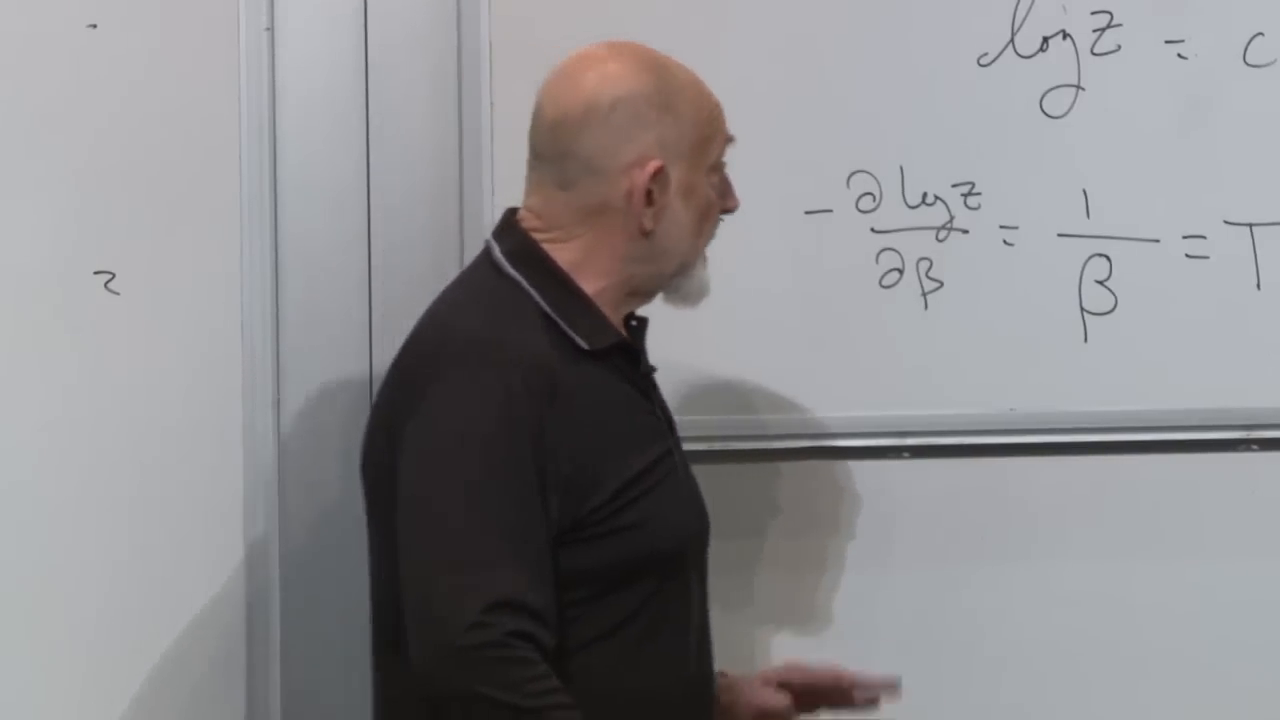
\includegraphics[width=0.90\textwidth]{lecture_07_figure_02.png}
\caption{Вместе показаны оценка по молекулярной скорости, производная давления и подстановка для идеального газа.}
\lectureframe{00:08:55}
\end{figure}

Есть важное уточнение. Звуковая волна малой амплитуды обычно сжимает и разрежает газ быстрее, чем тепло успевает перетекать между соседними элементами. Поэтому локальное движение приблизительно адиабатично, а не изотермично:
\begin{equation}
 c_s^2=
 \left(\frac{\partial P}{\partial\rho_m}\right)_S.
 \label{eq:sm7-sound-adiabatic}
\end{equation}
Для идеального газа с адиабатическим показателем \(\gamma\),
\begin{equation}
 P\rho_m^{-\gamma}=\text{constant},
 \qquad
 c_s^2=\gamma\frac{P}{\rho_m}
       =\gamma\frac{k_B T}{m}.
 \label{eq:sm7-sound-ideal-adiabatic}
\end{equation}
Для двухатомного воздуха при комнатной температуре \(\gamma\simeq 7/5\). Таким образом, расчёт при фиксированной температуре даёт полезную первую оценку, тогда как адиабатическая производная даёт физически правильное уточнение.

Используя грубые значения
\begin{equation}
\begin{aligned}
 k_B&\simeq1.3\times10^{-23}\ {\rm J\,K^{-1}},
 &T&\simeq300\ {\rm K},\\
 m_{\rm air}&\simeq4\times10^{-26}\ {\rm kg}.&&
\end{aligned}
 \label{eq:sm7-air-data}
\end{equation}
получаем, что молекулярная оценка составляет примерно \(500\ {\rm m\,s^{-1}}\). Температура здесь должна быть абсолютной температурой в кельвинах, а не шкалой со смещённым нулём, такой как шкала Фаренгейта. Привычная скорость звука имеет порядок \(300\ {\rm m\,s^{-1}}\), а адиабатическая формула идеального газа даёт при комнатной температуре около \(340\ {\rm m\,s^{-1}}\). Следовательно, грубый расчёт действительно нашёл правильный физический масштаб.

\begin{figure}[t]
\centering
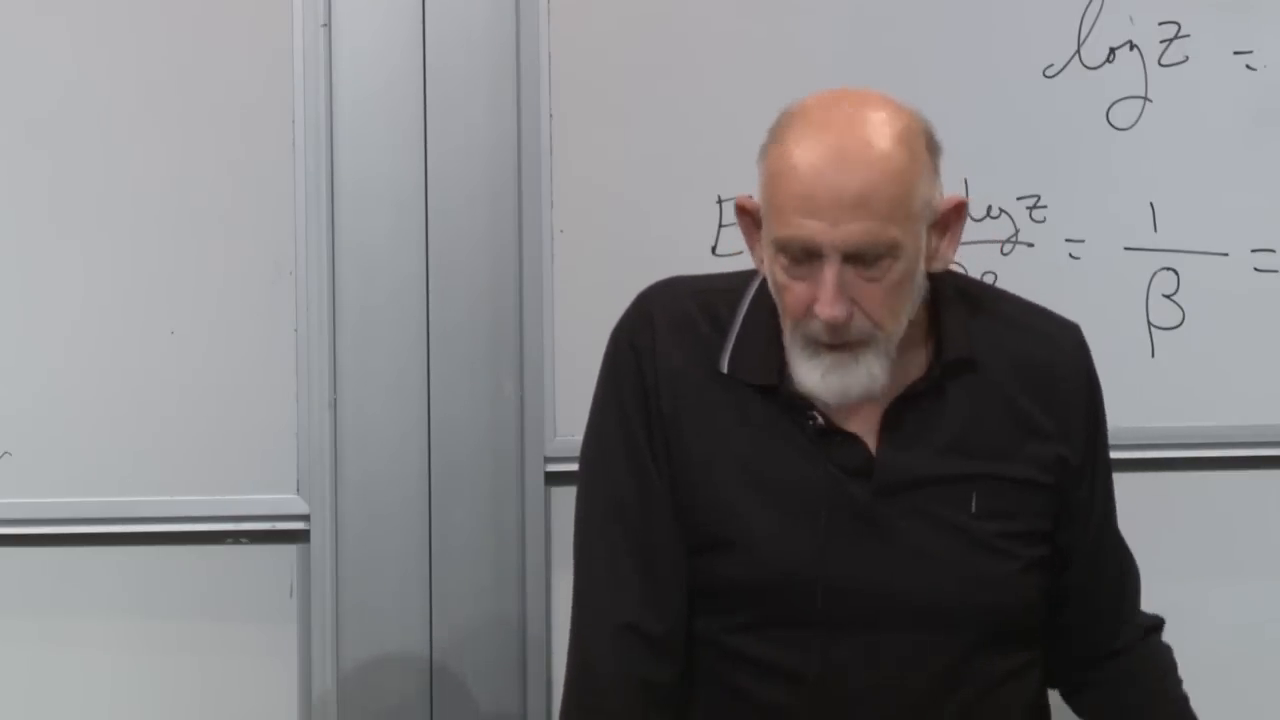
\includegraphics[width=0.90\textwidth]{lecture_07_figure_03.png}
\caption{Оценка для комнатного воздуха с использованием постоянной Больцмана, эффективной молекулярной массы около \(30\) протонных масс и \(T\simeq300\ {\rm K}\).}
\lectureframe{00:10:55}
\end{figure}

Задолго до появления микроскопического описания скорость звука можно было определять по измерениям зависимости давления от плотности. Статистический аргумент добавляет поразительную интерпретацию: получающаяся макроскопическая скорость задаётся тепловой скоростью отдельных молекул.

\begin{classroomqa}
\audiencequestion{Следует ли добавлять нейтроны к молекулярной массе, и учитывает ли число \(14\) для азота только протоны?}
\lecturerresponse{Указанная атомная масса уже учитывает протоны и нейтроны. Молекулярный азот содержит два атома с атомной массой около \(14\), так что его масса составляет примерно \(28\) протонных масс; для этой оценки достаточно округлить \(28\) до \(30\).
\lecturetimestamp{00:10:58--00:11:16}}
\end{classroomqa}

\begin{classroomqa}
\audiencequestion{Множитель \(3\) появился из трёх поступательных направлений, тогда как звук распространяется вдоль одного направления. Не должно ли это убрать множитель \(3\)?}
\lecturerresponse{Это справедливо предупреждает нас, что не следует отождествлять трёхмерную среднеквадратичную молекулярную скорость с одномерной скоростью распространения. Исходный довод был лишь картиной на уровне порядка величины. Корректный ответ даёт производная давления вместе с термодинамическим условием, подходящим для данной волны.
\lecturetimestamp{00:11:12--00:12:00}}
\end{classroomqa}

\begin{classroomqa}
\audiencequestion{Предполагала ли эта производная, что во время волны температура остаётся постоянной?}
\lecturerresponse{Да, показанная подстановка для идеального газа именно это и предполагала. Фиксировать температуру — правдоподобная предварительная оценка для очень малого возмущения; стандартное уточнение состоит в том, что обычный звук приблизительно адиабатичен, и тогда изотермическая производная заменяется на \(\left(\partial P/\partial\rho_m\right)_S\).
\lecturetimestamp{00:12:59--00:14:01}}
\end{classroomqa}

\begin{classroomqa}
\audiencequestion{Если изменения давления и плотности оба малы, делает ли это их производную малой?}
\lecturerresponse{Нет. Производная — это отношение двух малых изменений в бесконечно малом пределе. И \(\delta P\), и \(\delta\rho\) могут быть малы, тогда как \(\delta P/\delta\rho\) остаётся конечным и задаёт скорость волны.
\lecturetimestamp{00:14:03--00:14:23}}
\end{classroomqa}

\begin{classroomqa}
\audiencequestion{Должна ли скорость звука возрастать при сжатии газа, как это происходит при переходе от газа к жидкости или твёрдому телу?}
\lecturerresponse{Да. Производная вычисляется в рассматриваемом состоянии, и \(P(\rho,T)\) не обязана оставаться линейной. Когда молекулы оказываются тесно сжаты, уравнение состояния становится неидеальным, и \(\partial P/\partial\rho\) может существенно возрасти.
\lecturetimestamp{00:14:25--00:15:13}}
\end{classroomqa}

\begin{classroomqa}
\audiencequestion{Можно ли значение \(500\ {\rm m\,s^{-1}}\) использовать при любом давлении?}
\lecturerresponse{Нет. Оно относится к области малых плотностей, где уравнение идеального газа служит полезным приближением. Как только в \(P(\rho,T)\) входят более высокие степени плотности, производная и, следовательно, скорость звука зависят от давления и плотности.
\lecturetimestamp{00:15:14--00:16:29}}
\end{classroomqa}

\begin{classroomqa}
\audiencequestion{Перестаёт ли работать и исходная картина, в которой звук распространяется примерно с молекулярной скоростью, по мере роста плотности?}
\lecturerresponse{Вероятно, да. Эта картина приспособлена к разрежённому газу. При большой плотности коллективные взаимодействия становятся всё важнее, и именно поэтому производная уравнения состояния даёт более общее описание.
\lecturetimestamp{00:16:32--00:16:53}}
\end{classroomqa}

\begin{classroomqa}
\audiencequestion{Почему массу молекулы азота записали как примерно \(30\) протонных масс, а не \(28\)?}
\lecturerresponse{Нужна лишь численная точность, соответствующая этой оценке, поэтому \(28\) было округлено до \(30\). Если разделить исходную оценку \(500\ {\rm m\,s^{-1}}\) на \(\sqrt{3}\simeq1.7\), тоже получается значение, близкое к \(300\ {\rm m\,s^{-1}}\), хотя адиабатическая производная — это корректный способ вычислить поправку.
\lecturetimestamp{00:16:54--00:17:27}}
\end{classroomqa}

\section{Один классический осциллятор в тепловой ванне}

Теперь мы заменим свободно поступательно движущуюся молекулу одним гармоническим осциллятором, а всё остальное будем рассматривать как тепловую ванну. Непосредственный образ — это масса на пружине, но модель гораздо шире. Колеблется мода электромагнитной полости; колеблются атомы в кристалле; почти всякая устойчивая система, слегка выведенная из равновесия, в ведущем приближении совершает гармоническое движение.

Если \(x\) отсчитывать от положения равновесия, а импульс, масса и коэффициент жёсткости пружины равны соответственно \(p\), \(m\) и \(\kappa\), то гамильтониан имеет вид
\begin{equation}
 H(x,p)=\frac{p^2}{2m}+\frac{\kappa x^2}{2},
 \qquad
 \omega=\sqrt{\frac{\kappa}{m}}.
 \label{eq:sm7-classical-hamiltonian}
\end{equation}
Тепловая ванна задаёт \(T\), и с этого места мы снова используем \(k_B=1\), так что \(\beta=1/T\). Осциллятор, пришедший в равновесие с комнатной средой, имеет температуру около \(300\ {\rm K}\); у осциллятора, погружённого в жидкий гелий, температура всего несколько кельвинов. Гипотетическая пружина, помещённая в центр Солнца, не уцелела бы как пружина, но этот пример ясно показывает роль окружающей среды. Больцмановский вес факторизуется:
\begin{equation}
 e^{-\beta H}
 =e^{-\beta p^2/(2m)}
  e^{-\beta\kappa x^2/2}.
 \label{eq:sm7-factorized-weight}
\end{equation}

\begin{figure}[t]
\centering
\includegraphics[width=0.90\textwidth]{lecture_07_figure_04.png}
\caption{Пружинный осциллятор и его гамильтониан как сумма кинетической и потенциальной энергий.}
\lectureframe{00:20:55}
\end{figure}

В отличие от свободного газа, интеграл по координате не просто даёт объём сосуда. Восстанавливающий потенциал взвешивает каждое смещение:
\begin{equation}
 Z_{\rm cl}
 =\frac{1}{h}\int_{-\infty}^{\infty}dp
             \int_{-\infty}^{\infty}dx\,
 e^{-\beta p^2/(2m)}
 e^{-\beta\kappa x^2/2}.
 \label{eq:sm7-classical-z}
\end{equation}
Множитель \(1/h\) делает одномерную классическую статистическую сумму безразмерной. В выкладке на доске он опущен, поскольку не зависит от \(\beta\) и не может влиять на среднюю энергию.

\begin{figure}[t]
\centering
\includegraphics[width=0.90\textwidth]{lecture_07_figure_05.png}
\caption{Классическая статистическая сумма осциллятора разложена на гауссовы интегралы по импульсу и смещению.}
\lectureframe{00:22:55}
\end{figure}

Для интеграла по импульсу положим
\begin{equation}
 q=\sqrt{\frac{\beta}{2m}}\,p,
 \qquad
 dp=\sqrt{\frac{2m}{\beta}}\,dq.
 \label{eq:sm7-p-gaussian-substitution}
\end{equation}
Для интеграла по координате положим
\begin{equation}
 y=\sqrt{\frac{\beta\kappa}{2}}\,x,
 \qquad
 dx=\sqrt{\frac{2}{\beta\kappa}}\,dy.
 \label{eq:sm7-x-gaussian-substitution}
\end{equation}
Поскольку \(\int_{-\infty}^{\infty}e^{-u^2}\,du=\sqrt{\pi}\), используемый на доске ненормированный интеграл по фазовому пространству равен
\begin{equation}
 \int dp\,dx\,e^{-\beta H}
 =\frac{2\pi}{\beta}\sqrt{\frac{m}{\kappa}}
 =\frac{2\pi}{\beta\omega}.
 \label{eq:sm7-classical-z-unnormalized}
\end{equation}
После восстановления ячейки фазового пространства получаем
\begin{equation}
 Z_{\rm cl}=\frac{2\pi}{h\beta\omega}
           =\frac{1}{\beta\hbar\omega}.
 \label{eq:sm7-classical-z-normalized}
\end{equation}

Для энергии важна только зависимость от \(\beta\):
\begin{equation}
 \begin{aligned}
 \log Z_{\rm cl}&=\text{constant}-\log\beta,\\
 \expect{H}
 &=-\frac{\partial\log Z_{\rm cl}}{\partial\beta}\\
 &=\frac{1}{\beta}=T.
 \end{aligned}
 \label{eq:sm7-classical-energy}
\end{equation}

\begin{figure}[t]
\centering
\includegraphics[width=0.90\textwidth]{lecture_07_figure_06.png}
\caption{Полная классическая цепочка на правой доске: гауссова факторизация, \(Z\propto(\beta\omega)^{-1}\) и \(\expect{H}=1/\beta=T\).}
\lectureframe{00:30:15}
\end{figure}

Множителя \(3\) нет, потому что это осциллятор в одном пространственном измерении. Остающегося множителя \(1/2\) тоже нет, потому что имеются два независимых квадратичных члена. Каждый гауссовский интеграл даёт \(T/2\):
\begin{equation}
 \expect{K}=\frac{T}{2},
 \qquad
 \expect{U}=\frac{T}{2},
 \qquad
 \expect{H}=T.
 \label{eq:sm7-equipartition-oscillator}
\end{equation}
Это равнораспределение в наиболее полезной форме: каждый независимый квадратичный член в классическом гамильтониане даёт вклад \(T/2\).

Полученный ответ не зависит ни от \(m\), ни от \(\kappa\). Само движение, однако, зависит от этих параметров:
\begin{equation}
 \expect{p^2}=mT,
 \qquad
 \expect{x^2}=\frac{T}{\kappa},
 \qquad
 \expect{\dot{x}^2}=\frac{T}{m}.
 \label{eq:sm7-classical-fluctuations}
\end{equation}
Поэтому более тяжёлая масса движется медленнее, а более жёсткая пружина имеет меньшую амплитуду, хотя средняя энергия остаётся равной \(T\).
Это начинает тревожить, когда \(\kappa\) делают фантастически большим. Пружина, слишком жёсткая, чтобы двигаться, должна выглядеть как замороженная связь, однако классическое равнораспределение всё равно приписывает ей энергию \(T\).

\begin{classroomqa}
\audiencequestion{При \(\kappa\to\infty\) статистическая сумма стремится к нулю. Как тогда всё же можно использовать её логарифм?}
\lecturerresponse{Держите \(\kappa\) конечным, но сколь угодно большим. Его вклад в \(\log Z\) аддитивен и не зависит от \(\beta\), так что производная по \(\beta\) по-прежнему даёт \(T\). Неудобство, связанное с этим предельным переходом, реально: классический расчёт внутренне согласован, но в нём отсутствует черта природы, необходимая для очень жёстких осцилляторов.
\lecturetimestamp{00:34:01--00:34:54}}
\end{classroomqa}

\begin{classroomqa}
\audiencequestion{Для статистической суммы идеального газа требовался множитель \(N!\). Должен ли быть здесь аналогичный факториал?}
\lecturerresponse{Нет. Мы изучаем один конкретно заданный осциллятор, а не переставляем \(N\) одинаковых частиц. Для многих независимых помеченных мод статистические суммы перемножаются. Фактор неразличимости относится к другой задаче подсчёта.
\lecturetimestamp{00:35:03--00:35:40}}
\end{classroomqa}

\section{Почему классическое равнораспределение обернулось кризисом}

Реальные молекулы не являются бесструктурными точками. Двухатомная молекула содержит связь, способную колебаться, а значит — внутренний осциллятор. Наивный классический подсчёт приписал бы этой моде дополнительную тепловую энергию даже при обычных температурах. В заведомо схематическом подсчёте включение одного колебательного осциллятора повышает энергию с \(3T/2\) к \(5T/2\). Точный учёт теплоёмкости должен также включать вращательные степени свободы и различать энергию и её производную по температуре. Решающий экспериментальный факт проще: жёсткие внутренние моды при низкой температуре не давали вклада, как того требовало классическое равнораспределение.

Можно либо отрицать, что молекула имеет внутреннюю структуру, что абсурдно, либо признать, что в классической механике не хватает некоторого ингредиента. Этим ингредиентом является квантовая механика. Нам нужно совсем немного: лишь то, что гармонический осциллятор имеет равноотстоящие энергетические уровни.

\section{Квантовый осциллятор}

Сначала сдвинем начало отсчёта энергии и запишем спектр возбуждений в виде
\begin{equation}
 E_n^{\rm exc}=n\hbar\omega,
 \qquad n=0,1,2,\ldots.
 \label{eq:sm7-shifted-spectrum}
\end{equation}
Теперь статистическая сумма представляет собой настоящую сумму, а не интеграл по фазовому пространству:
\begin{align}
 Z_{\rm exc}
 &=\sum_{n=0}^{\infty}e^{-\beta n\hbar\omega} \notag\\
 &=1+x+x^2+\cdots
  =\frac{1}{1-x},
 \qquad x=e^{-\beta\hbar\omega}, \notag\\
 &=\frac{1}{1-e^{-\beta\hbar\omega}}.
 \label{eq:sm7-quantum-z}
\end{align}

\begin{figure}[t]
\centering
\includegraphics[width=0.90\textwidth]{lecture_07_figure_07.png}
\caption{Равноотстоящие уровни и вычисление статистической суммы квантового осциллятора как геометрической прогрессии.}
\lectureframe{00:42:05}
\end{figure}

Дифференцирование даёт среднюю энергию возбуждения:
\begin{align}
 E_{\rm exc}
 &=-\frac{\partial\log Z_{\rm exc}}{\partial\beta}
  =-\frac{1}{Z_{\rm exc}}
    \frac{\partial Z_{\rm exc}}{\partial\beta}
 \notag\\
 &=\hbar\omega\,
   \frac{e^{-\beta\hbar\omega}}
        {1-e^{-\beta\hbar\omega}}
  =\frac{\hbar\omega}{e^{\beta\hbar\omega}-1}.
 \label{eq:sm7-quantum-energy}
\end{align}

\begin{figure}[t]
\centering
\includegraphics[width=0.90\textwidth]{lecture_07_figure_08.png}
\caption{Тепловая энергия возбуждения, полученная взятием производной по \(\beta\) от квантовой статистической суммы.}
\lectureframe{00:46:05}
\end{figure}

\subsection{Высокая температура}

Когда \(\beta\hbar\omega\ll1\),
\begin{equation}
 e^{-\beta\hbar\omega}
 =1-\beta\hbar\omega
  +O\!\left((\beta\hbar\omega)^2\right).
 \label{eq:sm7-high-t-expansion}
\end{equation}
Числитель в \eqref{eq:sm7-quantum-energy} стремится к \(\hbar\omega\), тогда как знаменатель в главном порядке равен \(\beta\hbar\omega\). Поэтому
\begin{equation}
 E_{\rm exc}\simeq\frac{1}{\beta}=T.
 \label{eq:sm7-high-t-energy}
\end{equation}
Квантовый ответ воспроизводит классическое равнораспределение, когда в тепловую энергию укладывается много межуровневых расстояний.

\subsection{Низкая температура}

Когда \(\beta\hbar\omega\gg1\), экспонента очень мала:
\begin{equation}
 E_{\rm exc}
 \simeq\hbar\omega e^{-\beta\hbar\omega}.
 \label{eq:sm7-low-t-energy}
\end{equation}
Тепловое возбуждение осциллятора экспоненциально подавлено. При сдвинутом выборе нуля энергии оно почти равно нулю; физическая энергия нулевых колебаний будет восстановлена ниже.

\begin{figure}[t]
\centering
\includegraphics[width=0.90\textwidth]{lecture_07_figure_09.png}
\caption{Низкотемпературное разложение: первое тепловое возбуждение подавлено фактором \(e^{-\beta\hbar\omega}\).}
\lectureframe{00:51:55}
\end{figure}

Переходная область возникает, когда
\begin{equation}
 \beta\hbar\omega\sim1,
 \qquad\text{or equivalently}\qquad
 T\sim\hbar\omega.
 \label{eq:sm7-crossover}
\end{equation}
У этого условия есть непосредственный смысл. Классическое равнораспределение дало бы осциллятору энергию \(T\). Квантовые эффекты становятся неизбежными, когда этот масштаб оказывается меньше расстояния между соседними уровнями. Следовательно,
\begin{equation}
\begin{aligned}
 \hbar\omega\gg T&:\quad \text{frozen and quantum},\\
 \hbar\omega\ll T&:\quad \text{active and classical}.
\end{aligned}
 \label{eq:sm7-regimes}
\end{equation}
Более жёсткая пружина имеет большее \(\omega=\sqrt{\kappa/m}\), поэтому для классического поведения ей требуется более высокая температура.

\section{Степени свободы проявляются по мере нагревания вещества}

При низкой температуре двухатомная молекула может в тепловом отношении напоминать точечную частицу, потому что колебание её жёсткой связи выморожено. Когда \(T\) возрастает и проходит через \(\hbar\omega\), колебательная мода активируется. Вращательные моды могут активироваться на меньшем масштабе; при ещё более высоких температурах проявляется больше внутреннего движения, а в конце концов происходит ионизация атома. Нагревание не просто вкладывает больше энергии в фиксированный список мод. Оно выявляет степени свободы, которые при более низкой температуре были невидимы.

Воображаемая вложенная молекула делает эту мысль нагляднее. Два атома соединены жёсткой пружиной, а один кажущийся атом сам представляет собой пару, соединённую ещё более жёсткой пружиной. При низкой \(T\) обе структуры выглядят точечными. При первом пороге появляется внешнее колебание; при втором — внутренняя структура. Сложность системы раскрывается по одному энергетическому масштабу за раз.

\begin{classroomqa}
\audiencequestion{Если осциллятор уже находится в классическом режиме, делает ли дальнейший нагрев пружину более жёсткой или изменяет её частоту?}
\lecturerresponse{Нет. Жёсткость пружины и частота остаются фиксированными. Более высокая температура приводит к большим типичным импульсам и амплитудам, а значит, и к большей энергии. Жёсткость определяет температуру, при которой классический закон начинает работать, а не приводит к зависящему от температуры увеличению жёсткости пружины.
\lecturetimestamp{01:03:17--01:05:11}}
\end{classroomqa}

\subsection{Кристаллы и удельная теплоёмкость Эйнштейна}

Кристалл содержит очень много колебательных мод. Классическое равнораспределение приписывает каждому активному осциллятору энергию порядка \(T\) и потому завышает низкотемпературную теплоёмкость. Модель Эйнштейна 1907 года рассматривала колебания кристалла квантовомеханически и показала, почему они подавлены, пока тепловая энергия не достигает их межуровневого расстояния. Более точные модели твёрдого тела допускают распределение частот мод, но принцип вымораживания уже присутствует в расчёте Эйнштейна.

\begin{classroomqa}
\audiencequestion{Была ли это именно та работа, за которую Эйнштейн получил Нобелевскую премию, и появилась ли она только после того, как квантовая механика уже установилась?}
\lecturerresponse{Нет. В нобелевской формулировке речь шла о фотоэффекте. Модель теплоёмкости была опубликована в 1907, задолго до того, как были поняты полные основания квантовой механики. Эйнштейн принял и развил ключевые квантовые идеи, хотя позднее и возражал против некоторых сторон зрелой теории.
\lecturetimestamp{00:58:38--01:03:16}}
\end{classroomqa}

\begin{classroomqa}
\audiencequestion{В классической статистической механике сумма по дискретным состояниям заменяется, по-видимому, равномерным интегралом по координате и импульсу. Чем оправдан такой подсчёт состояний?}
\lecturerresponse{Окончательное обоснование даёт квантовая механика. В высокотемпературном пределе
\[
 Z_{\rm exc}\simeq\frac{1}{\beta\hbar\omega},
\]
что в точности совпадает с безразмерным классическим результатом \eqref{eq:sm7-classical-z-normalized}. Квантовые ячейки фазового пространства переходят в классическую меру, когда межуровневое расстояние уже не разрешается.
\lecturetimestamp{00:59:38--01:03:06}}
\end{classroomqa}

\subsection{Струна содержит бесконечно много осцилляторов}

Струна скрипки или гитары разлагается на нормальные моды: основную моду, высшие гармоники и моды со всё более короткими длинами волн. Математически существует бесконечно много осцилляторных мод. Если бы классическое равнораспределение приписывало каждой из них энергию \(T\), то струна в тепловом равновесии имела бы бесконечную энергию. Квантовая механика предотвращает эту катастрофу. Моды с самыми короткими длинами волн имеют наибольшие частоты и остаются замороженными при любой конечной температуре; по мере роста \(T\) активируется всё больше мод. Та же логика позже ляжет в основу излучения абсолютно чёрного тела.

\begin{figure}[t]
\centering
\includegraphics[width=0.90\textwidth]{lecture_07_figure_10.png}
\caption{Наложение нескольких нормальных мод на струне, иллюстрирующее, почему непрерывная струна представляет собой бесконечное множество гармонических осцилляторов.}
\lectureframe{01:09:30}
\end{figure}

\begin{classroomqa}
\audiencequestion{Можно ли непосредственно наблюдать переход от квантового к классическому режиму, и может ли нагрев обратить вспять низкотемпературное поведение?}
\lecturerresponse{Да. Температурная зависимость удельной теплоёмкости кристалла делает вымораживание и последующую активацию колебательных мод отчётливо измеримыми.
\lecturetimestamp{01:09:11--01:10:13}}
\end{classroomqa}

\begin{classroomqa}
\audiencequestion{Для многих осцилляторов нужно ли для каждой моды брать статистическую сумму одного осциллятора?}
\lecturerresponse{Для независимых мод,
\[
\begin{aligned}
 Z_{\rm tot}&=\prod_j Z_j,&
 \log Z_{\rm tot}&=\sum_j\log Z_j,\\
 E_{\rm tot}&=\sum_j E_j.&&
\end{aligned}
\]
Моды с \(\hbar\omega_j\gg T\) дают экспоненциально малый тепловой вклад; моды ниже этого порога вносят заметный вклад.
\lecturetimestamp{01:10:14--01:11:00}}
\end{classroomqa}

\begin{classroomqa}
\audiencequestion{Что произошло с энергией нулевых колебаний осциллятора \(\hbar\omega/2\)?}
\lecturerresponse{Физические уровни имеют вид
\[
 E_n=\left(n+\frac12\right)\hbar\omega.
\]
Следовательно
\[
 \begin{aligned}
 Z_{\rm phys}
 &=e^{-\beta\hbar\omega/2}Z_{\rm exc},\\
 E_{\rm phys}
 &=\frac{\hbar\omega}{2}
  +\frac{\hbar\omega}{e^{\beta\hbar\omega}-1}.
 \end{aligned}
\]
Общий сдвиг не изменяет вероятностей уровней, энтропии, теплоёмкости или тепловой энергии возбуждения, но сдвигает абсолютную среднюю энергию на \(\hbar\omega/2\). Множитель в \(Z\) зависит от \(\beta\), поэтому, когда нужна абсолютная энергия, его нельзя отбрасывать.
\lecturetimestamp{01:11:08--01:11:37}}
\end{classroomqa}

\section{Второй закон как парадокс обратимости}

Теперь мы можем вернуться к обещанной проблеме. Второй закон утверждает, что обычная макроскопическая эволюция необратима и что энтропия имеет тенденцию возрастать. Микроскопическая гамильтонова эволюция обратима. Как обратимое отображение точных состояний может породить необратимый закон для макроскопических состояний?

Представим систему точкой в фазовом пространстве высокой размерности,
\[
 \Gamma=(q_1,\ldots,q_N,p_1,\ldots,p_N).
\]
Наше знание обычно не задаётся точной точкой. Предположим, что оно задаётся равномерной плотностью вероятности на компактной области \(A\) объёма \(\Omega_A\):
\begin{equation}
 f(\Gamma)=
 \begin{cases}
  1/\Omega_A,&\Gamma\in A,\\
  0,&\Gamma\notin A.
 \end{cases}
 \label{eq:sm7-uniform-blob}
\end{equation}
В единицах, где \(k_B=1\), её мелкозернистая энтропия Гиббса равна
\begin{equation}
 S_{\rm fine}
 =-\int d\Gamma\,f\log f
 =\log\Omega_A.
 \label{eq:sm7-blob-entropy}
\end{equation}
Меньшая область означает больше информации и меньшую энтропию. Это определяет знак: рост неопределённости увеличивает занятую область и повышает \(\log\Omega_A\).

\begin{figure}[t]
\centering
\includegraphics[width=0.90\textwidth]{lecture_07_figure_11.png}
\caption{Компактная вероятностная область в схематическом двумерном сечении полного фазового пространства координат и импульсов.}
\lectureframe{01:20:20}
\end{figure}

\begin{classroomqa}
\audiencequestion{Физически ли система ограничена тем, что должна оставаться внутри нарисованной области, и находится ли она уже в равновесии?}
\lecturerresponse{Нет. Эта область описывает то, что известно о начальном состоянии, а не стенку в фазовом пространстве. Она не обязана быть равновесным распределением. Газ, первоначально заключённый в баке в одном углу комнаты, — конкретный пример специальной неравновесной информации.
\lecturetimestamp{01:14:55--01:15:24}}
\end{classroomqa}

\section{Поток Лиувилля и рост при грубом зернении}

Теорема Лиувилля утверждает, что гамильтонов поток сохраняет фазовый объём. Точная область может смещаться, растягиваться, складываться и становиться чрезвычайно тонкой, но
\begin{equation}
 \Omega_{A(t)}=\Omega_{A(0)},
 \qquad
 S_{\rm fine}(t)=S_{\rm fine}(0).
 \label{eq:sm7-liouville}
\end{equation}
Дискретный аналог — обратимая перестановка состояний. Если вначале известно, что игральная кость находится в одном из двух состояний, то взаимно-однозначная эволюция может изменить, какие именно это два состояния, но не число возможностей.

Реальные описания имеют конечное разрешение. Квантовая механика задаёт естественную ячейку фазового пространства, а классический эксперимент обладает конечной точностью измерений даже без обращения к квантовой теории. Под действием гамильтонова потока область может превратиться в длинную тонкую змейку. Если расстояние между соседними складками становится меньше масштаба разрешения, мы заменяем каждую неразрешённую окрестность грубой ячейкой. Точный занятый объём остаётся неизменным, но объединение грубых ячеек растёт:
\begin{equation}
 \Omega_{\rm coarse}(t)\geq\Omega_{A(t)},
 \qquad
 S_{\rm coarse}(t)=\log\Omega_{\rm coarse}(t).
 \label{eq:sm7-coarse-entropy}
\end{equation}

\begin{figure}[t]
\centering
\includegraphics[width=0.90\textwidth]{lecture_07_figure_12.png}
\caption{Объёмосохраняющий филамент, рассматриваемый через ячейки конечного разрешения. Точный чёрный филамент сохраняет свою площадь; красные грубые ячейки занимают большую эффективную область.}
\lectureframe{01:22:10}
\end{figure}

\begin{classroomqa}
\audiencequestion{Грубые ячейки перекрываются. Не нарушает ли это теорему Лиувилля?}
\lecturerresponse{Нет. Теорема Лиувилля относится к точному филаменту, который по-прежнему описывается взаимно-однозначной объёмосохраняющей эволюцией. Перекрытие относится к нашему размытому описанию: мы отбросили информацию о том, какая из тонких нитей содержит состояние.
\lecturetimestamp{01:21:32--01:21:50}}
\end{classroomqa}

Полезная аналогия — вата. Суммарный материальный объём всех волокон может оставаться почти постоянным, тогда как распушённый комок занимает большой кажущийся объём для наблюдателя, не способного различить отдельные волокна. Аналогично область в фазовом пространстве отращивает всё более тонкие щупальца; у них, в свою очередь, возникают ещё более тонкие щупальца. Любое фиксированное конечное разрешение рано или поздно перестаёт их отслеживать.

\begin{classroomqa}
\audiencequestion{Получается, что в классике энтропия лишь кажется возрастающей, а квантовая механика делает этот рост реальным, вводя фундаментальный предел разрешения?}
\lecturerresponse{Аргумент с грубым зернением не требует квантового предела. Энтропия относится одновременно к системе и к тем макроскопическим различиям, которые сохраняются в её описании. При бесконечной микроскопической информации мелкозернистая энтропия постоянна; при любом фиксированном конечном разрешении хаотические филаменты со временем становятся неразличимыми, и грубозернистая энтропия возрастает.
\lecturetimestamp{01:24:04--01:25:20}}
\end{classroomqa}

\section{Хаос, конечная доступная область и установление равновесия}

Для газа в ящике координаты ограничены. При фиксированной конечной полной энергии импульсы тоже ограничены, даже если вся энергия на мгновение сосредоточена в одной частице. Поэтому при обычных предположениях об ограниченности системы динамически доступная энергетическая оболочка имеет конечную меру.

\begin{figure}[t]
\centering
\includegraphics[width=0.90\textwidth]{lecture_07_figure_13.png}
\caption{Ограниченная доступная область фазового пространства рядом с филаментом и его грубозернистым представлением.}
\lectureframe{01:28:10}
\end{figure}

Близкие начальные точки в хаотической системе некоторое время проходят сходные истории, а затем расходятся. При разбое в бильярде незаметное изменение направления битка воспроизводится в последующих соударениях; различия накапливаются, пока конечные конфигурации не перестают быть связанными друг с другом. Поэтому вся начальная область растягивается и складывается по всей доступной области. При конечном разрешении она приближается к широкому, почти однородному равновесному описанию.

\begin{figure}[t]
\centering
\includegraphics[width=0.90\textwidth]{lecture_07_figure_14.png}
\caption{Компактное специальное состояние эволюционировало в сложный филамент, протянувшийся по ограниченной доступной области, тогда как грубозернистые ячейки распространились по гораздо большей площади.}
\lectureframe{01:33:10}
\end{figure}

Важны две оговорки. Сам по себе хаос не доказывает, что каждая траектория посещает любую доступную окрестность; для этого более сильного утверждения требуется эргодичность или свойство перемешивания. И не всякая физическая система хаотична. Типичный многочастичный газ и идеализированные бильярды дают именно ту постановку, которая здесь имеется в виду, где перемешивание является полезным физическим ожиданием.

\section{Возврат не отменяет необратимости}

Предположим, что все молекулы воздуха сначала находятся в одном углу и имеют специально подготовленную конфигурацию скоростей. Столкновения быстро распределяют их по комнате, и грубозернистое описание достигает равновесия. В фазовом пространстве с конечной мерой, сохраняемой эволюцией, теорема Пуанкаре о возврате утверждает, что почти всякая начальная точка возвращается сколь угодно близко к своей исходной точке. При допуске \(\epsilon>0\) время возврата \(t_R(\epsilon)\) конечно при выполнении гипотез теоремы, хотя для макроскопической системы оно фантастически велико. Точный возврат в бесконечно точно заданную точку не требуется и, вообще говоря, не ожидается.

\begin{classroomqa}
\audiencequestion{В примере с бильярдом не вносит ли удар по битку энергию и не нарушает ли этим замкнутую эволюцию?}
\lecturerresponse{Выбранное начальное состояние задаётся сразу после удара, когда эта энергия уже учтена. Возврат относится к последующей изолированной динамике идеализированного бильярда; возврат вблизи начального состояния включает конфигурацию, эквивалентную тому, что биток приближается к пирамиде в пределах выбранного допуска.
\lecturetimestamp{01:35:37--01:35:55}}
\end{classroomqa}

\begin{classroomqa}
\audiencequestion{Если газ в конце концов может вернуться в угол, значит ли это, что мы потеряли информацию, и действительно ли система обратима?}
\lecturerresponse{Микроскопическая динамика всё время остаётся обратимой. Грубозернистая энтропия может возрастать, потому что мы перестаём различать тонкие корреляции, и всё же исключительно редкая флуктуация может вернуть систему вблизи её особого начального макросостояния. Следовательно, возврат и грубозернистая необратимость совместимы.
\lecturetimestamp{01:37:34--01:38:15}}
\end{classroomqa}

Это приводит к существенной формулировке Больцмана. Энтропия не возрастает в каждый логически возможный момент. Для неравновесного макросостояния большой системы подавляюще больше совместимых микроскопических продолжений ведут к более крупным макросостояниям, чем к ещё более специальным. Энтропия \emph{вероятно} возрастает. Нисходящие флуктуации и возвраты допустимы, но их вероятности и временные масштабы делают их невидимыми в обычном макроскопическом опыте. Проблема обратимости была одной из великих исторических проблем статистической механики и тяжело давила на Больцмана. Эту историческую связь не следует превращать в простое причинное утверждение о его жизни.

\section{Что означает хаос}

Для более операционального определения хаоса предположим, что две начальные точки фазового пространства различаются на \(\delta\Gamma(0)\); тогда в хаотическом направлении обычно имеет место
\begin{equation}
 \lVert\delta\Gamma(t)\rVert
 \sim e^{\lambda t}\lVert\delta\Gamma(0)\rVert,
 \qquad \lambda>0,
 \label{eq:sm7-lyapunov-growth}
\end{equation}
в том режиме, где осмысленно линеаризованное расхождение. Число \(\lambda\) — показатель Ляпунова. Чтобы предсказывать для времени \(t\), требуемая точность начальных данных масштабируется примерно как \(e^{-\lambda t}\). Точность задания динамического закона тоже важна: ошибки модели усиливаются вместе с ошибками в начальных условиях. Погода — привычный пример.

\begin{classroomqa}
\audiencequestion{Существует ли принцип, утверждающий, что \emph{большинство} систем хаотичны, или это лишь эмпирическое наблюдение?}
\lecturerresponse{Существует бесконечно много хаотических и нехаотических гамильтонианов, и даже слово \emph{большинство} требует меры на пространстве гамильтонианов. Сложные взаимодействующие системы часто хаотичны, но простого универсального теста, который позволял бы при простом рассмотрении классифицировать любой гамильтониан, не существует.
\lecturetimestamp{01:39:27--01:40:49}}
\end{classroomqa}

\begin{classroomqa}
\audiencequestion{Что именно означает слово \emph{хаотический} в этом обсуждении?}
\lecturerresponse{Близкие фазовые траектории расходятся достаточно быстро, так что для долговременного предсказания требуется экспоненциально растущая точность задания начальных условий. Гармонический осциллятор служит контрастным примером: соседние фазовые точки вращаются вместе и остаются близкими. Точная задача Кеплера двух тел также нехаотична, тогда как общая задача трёх тел имеет хаотические режимы.
\lecturetimestamp{01:40:50--01:43:45}}
\end{classroomqa}

\begin{classroomqa}
\audiencequestion{Должны ли законы движения, как и начальные условия, быть известны с высокой точностью?}
\lecturerresponse{Да. Оба источника ошибок проходят через динамику, и хаотическая эволюция усиливает оба.
\lecturetimestamp{01:43:46--01:43:55}}
\end{classroomqa}

Двойной маятник даёт наглядный пример. Обычный маятник интегрируем и предсказуем. Если добавить второй маятник, то траектории, начинающиеся почти вместе, со временем могут по-разному передавать энергию и направиться в совершенно разные стороны.

\begin{figure}[t]
\centering
\includegraphics[width=0.90\textwidth]{lecture_07_figure_15.png}
\caption{Двойной маятник как конкретный пример детерминированного хаоса.}
\lectureframe{01:44:40}
\end{figure}

\begin{classroomqa}
\audiencequestion{Почему одна механическая система может быть хаотической, а другая — нет?}
\lecturerresponse{Это свойство гамильтониана и его инвариантных структур, а не следствие трения или экспериментального шума. Математически установить это может быть трудно; сложность наводит на мысль, но не является доказательством.
\lecturetimestamp{01:44:03--01:45:58}}
\end{classroomqa}

\begin{classroomqa}
\audiencequestion{Остаётся ли идеальный двойной маятник хаотическим при отсутствии трения?}
\lecturerresponse{Да. Диссипация не требуется. Точное детерминированное гамильтоново движение может обладать чувствительной зависимостью от начальных условий. Начальные данные бесконечной точности определяли бы траекторию неограниченно долго, но конечная точность даёт конечный горизонт предсказуемости.
\lecturetimestamp{01:45:57--01:47:54}}
\end{classroomqa}

\begin{classroomqa}
\audiencequestion{Совпадает ли хаос с отсутствием решения в замкнутой форме?}
\lecturerresponse{Нет. У хаотических систем, как правило, нет глобально полезного выражения траектории в замкнутой форме, но аналитическая разрешимость и чувствительная зависимость — разные свойства. Хаос диагностируется динамически по расхождению траекторий, а не просто нашей неспособностью записать формулу.
\lecturetimestamp{01:48:20--01:49:23}}
\end{classroomqa}

\begin{classroomqa}
\audiencequestion{Чем широко распространённый хаос отличается от точного удержания равновесия на неустойчивой вершине холма?}
\lecturerresponse{Вершина холма — одно исключительное неустойчивое состояние: вдали от неё близкие траектории не обязаны быстро расходиться. В хаотической области неустойчивость типична вдоль орбиты, и близкие фазовые точки многократно расходятся. Положительный показатель Ляпунова характеризует это постоянное нарастание.
\lecturetimestamp{01:49:27--01:50:11}}
\end{classroomqa}

\section{От микроскопического движения к статистическому закону}

Оценка скорости звука показала, как микроскопическое тепловое движение задаёт макроскопический масштаб распространения, а вопросы выявили, какую именно термодинамическую производную нужно указать. Затем осциллятор показал, где классическое равнораспределение применимо, а где оно не работает. Квантовое расстояние между уровнями замораживает жёсткие моды, объясняет, почему теплоёмкости меняются с температурой, и не позволяет бесконечно многим высокочастотным модам нести бесконечную тепловую энергию.

Тот же переход от точной микрофизики к эффективному макроскопическому описанию разрешает кажущееся противоречие, лежащее в основе второго начала. Гамильтонов поток сохраняет точный объём фазового пространства и остаётся обратимым. Хаотическое растяжение создаёт более тонкие корреляции, чем сохраняет макроскопическое описание, поэтому в огрублённом описании занятая область растёт. Возвратность гарантирует, что редкие возвращения не запрещены; вероятность объясняет, почему они не определяют обычный опыт. Второе начало — не новая необратимая микроскопическая сила. Это чрезвычайно надёжное статистическое направление эволюции для специальных макроскопических начальных условий в системах с огромным числом степеней свободы.
\chapter{Возвраты, неравновесный порядок и спины Изинга}

\lectureoverview{Газ, выпущенный из одной половины комнаты, быстро устремляется к равновесию, однако обратимая механика говорит, что при достаточно долгой эволюции должны происходить и возвраты в это особое состояние. Мы оценим время такого возврата по объёму фазового пространства, отделим это явление от необъяснённого низкоэнтропийного начала Вселенной и используем возникающую отсюда загадку, чтобы обсудить мозги Больцмана, согласованную историю и жизнь, поддерживаемую потоком энергии. Затем мы перейдём к магнитному порядку. Независимые спины с двумя состояниями дают точно решаемый подготовительный пример: комбинаторика определяет статистическую сумму, а намагниченность выражается гиперболическим тангенсом. Взаимодействия между соседями, наконец, восстанавливают симметрию вверх--вниз и приводят к одномерной модели Изинга.}

\section{Воздух в комнате, который в конце концов возвращается}

Начнём с того, что весь воздух находится в левой половине комнаты. Такое состояние можно подготовить с помощью перегородки: откачать воздух из правой половины, поместить его слева, а затем убрать перегородку. Газ быстро распространяется по комнате и приближается к тепловому равновесию. Энтропия возрастает. Ничего удивительного не произошло.

Теперь оставим комнату герметично закрытой и подождём. Миллион орлов подряд — чрезвычайно маловероятный результат серии подбрасываний монеты, но в эксперименте, повторяемом неограниченно долго, рано или поздно возникают и чрезвычайно маловероятные результаты. Та же логика применима и к газу. В какой-то очень далёкий момент все его молекулы снова окажутся в левой половине или в какой-нибудь столь же особой области. Такое возвращение — это возврат Пуанкаре.

Точная теорема сформулирована несколько аккуратнее, чем эта наглядная картина. Для области фазового пространства конечной меры при динамике, сохраняющей объём фазового пространства, почти всякая начальная точка возвращается сколь угодно близко к своему исходному положению. Макроскопическое утверждение вроде \emph{все молекулы находятся в левой половине} проще: оно требует лишь, чтобы траектория снова вошла в конечную огрублённую область, а не чтобы каждая молекулярная координата вернулась в точности. Практический вопрос состоит в том, сколько времени это занимает.

\subsection{Фазовая точка высокой размерности}

Для \(N\) классических частиц фазовое пространство имеет \(6N\) координат,
\begin{equation}
 \Gamma=(\bm x_1,\ldots,\bm x_N;\bm p_1,\ldots,\bm p_N).
 \label{eq:sm8-phase-point}
\end{equation}
Положения ограничены комнатой. При фиксированной полной энергии импульсы тоже ограничены, потому что одна частица не может нести сколь угодно большой импульс, не неся сколь угодно большой энергии. Поэтому допустимая энергетическая оболочка имеет конечную меру при тех предположениях, которые используются в рассуждении о возврате.

Фазовая точка движется детерминированно, но в многочастичном газе её движение хаотично. Близкие траектории быстро расходятся, как это происходит в последовательности столкновений бильярдных шаров. После огрубления длинная траектория кажется блуждающей по всей доступной области.

\begin{figure}[t]
\centering
\includegraphics[width=0.90\textwidth]{lecture_08_figure_02.png}
\caption{Схематическая область фазового пространства и сложная траектория, блуждающая по ней. Рисунок намеренно сделан низкоразмерным; реальный газ живёт в \(6N\)-мерном пространстве.}
\lectureframe{00:06:41}
\end{figure}

Низкоразмерный набросок сразу же подталкивает нас к ошибке. Если бы особое состояние занимало половину изображённого прямоугольника, можно было бы сказать, что газ должен проводить там половину времени. Но условие \emph{каждая молекула лежит в левой половине} накладывает ограничение на каждую координату положения, а не только на одну координату фазовой точки.

Возьмём всего две частицы, движущиеся в одном пространственном измерении, с координатами \(x_1\) и \(x_2\). Их конфигурационное пространство — квадрат. Условие \(x_1<L/2\) отбирает половину квадрата; условия \(x_1<L/2\) и \(x_2<L/2\) вместе отбирают одну четверть:
\begin{equation}
 P_2=\frac{1}{2}\frac{1}{2}=\frac{1}{4}.
 \label{eq:sm8-two-particle-quarter}
\end{equation}

\begin{figure}[t]
\centering
\includegraphics[width=0.90\textwidth]{lecture_08_figure_07.png}
\caption{Для двух одномерных частиц меньший квадрат представляет конфигурации, в которых обе координаты лежат в выбранной половине комнаты.}
\lectureframe{00:07:08}
\end{figure}

Для трёх частиц получаем \(1/2^3\), а для \(N\) частиц получаем
\begin{equation}
 P_{\mathrm{half}}(N)
 =\left(\frac{1}{2}\right)^N.
 \label{eq:sm8-half-probability}
\end{equation}
Весь смысл именно в показателе степени. Множитель одна вторая вполне обычен; одна вторая в степени макроскопического числа частиц выходит за пределы обычной интуиции.

\begin{classroomqa}
\audiencequestion{Разве ответ не должен быть \(1/3^N\), ведь у молекул есть и другие пространственные направления?}
\lecturerresponse{Это зависит от того, какое условие налагается. Если единственный вопрос состоит в том, лежит ли каждая частица слева от разделяющей стенки, то для каждой частицы это одно двоичное условие, и ответ равен \(2^{-N}\). Наложение ограничения ещё на одну независимую долю её доступного пространства положений дало бы ещё один множитель.
\lecturetimestamp{00:07:47--00:08:05}}
\end{classroomqa}

\section{Фазовый объём, энтропия и масштаб возврата}

Ту же оценку можно записать и без обращения к половинам. Пусть комната имеет обычный пространственный объём \(V\), а \(v\) — меньшая область, в которой мы требуем, чтобы находилась каждая молекула. Пренебрегая импульсными множителями, общими для двух макросостояний, получаем для доступных объёмов конфигурационного пространства
\begin{equation}
 \Omega_{\mathrm{room}}\propto V^N,
 \qquad
 \Omega_{\mathrm{small}}\propto v^N.
 \label{eq:sm8-config-volumes}
\end{equation}
Поэтому доля долгого времени, проводимая в малом макросостоянии, равна
\begin{equation}
 P(v)
 =\frac{\Omega_{\mathrm{small}}}{\Omega_{\mathrm{room}}}
 =\left(\frac{v}{V}\right)^N.
 \label{eq:sm8-volume-ratio}
\end{equation}

\begin{figure}[t]
\centering
\includegraphics[width=0.90\textwidth]{lecture_08_figure_08.png}
\caption{Общая схема фазовых объёмов на доске: малая область \(v^N\) внутри доступной области \(V^N\), с отношением \(v^N/V^N\).}
\lectureframe{00:10:44}
\end{figure}

В единицах, где \(k_B=1\), энтропия есть логарифм доступного фазового объёма. Если \(S_A=\log\Omega_A\) — энтропия ограниченного макросостояния, а \(S_{\rm eq}=\log\Omega_{\rm eq}\) — энтропия равновесия, то
\begin{equation}
 \begin{aligned}
 P(A)
 &=\frac{\Omega_A}{\Omega_{\rm eq}}\\
 &=\exp\!\left(S_A-S_{\rm eq}\right)\\
 &=e^{-\Delta S},\\
 \Delta S&=S_{\rm eq}-S_A.
 \end{aligned}
 \label{eq:sm8-entropy-probability}
\end{equation}
Для случая полкомнаты \(\Delta S=N\log 2\), и
\eqref{eq:sm8-entropy-probability} в точности сводится к \(2^{-N}\).
Сокращённая запись \(P\sim e^{-S_{\rm eq}}\) уместна только тогда, когда энтропия особой области рассматривается как фиксированный эталон; физически осмысленным показателем степени является дефицит энтропии \(\Delta S\).

\begin{classroomqa}
\audiencequestion{Это объём конфигурационного пространства, а не всего фазового пространства?}
\lecturerresponse{Для этого сравнения — да. Мы накладываем условие на положения, оставляя распределение по импульсам при той же температуре, поэтому общий множитель из пространства импульсов сокращается. Полностью общее утверждение о возврате использует фазовое пространство; эту конкретную вероятность можно вычислить из отношения объёмов конфигурационного пространства.
\lecturetimestamp{00:11:21--00:11:40}}
\end{classroomqa}

Предположим, что система теряет память о своём детальном положении за микроскопическое время корреляции или перемешивания \(\tau_{\rm mix}\). Тогда попадание в редкую область с вероятностью \(P(A)\) происходит на масштабе
\begin{equation}
 \tau_{\rm rec}
 \sim \frac{\tau_{\rm mix}}{P(A)}
 \sim \tau_{\rm mix}e^{\Delta S}.
 \label{eq:sm8-recurrence-time-general}
\end{equation}
Для условия полкомнаты
\begin{equation}
 \tau_{\rm rec}\sim\tau_{\rm mix}2^N.
 \label{eq:sm8-recurrence-time-half}
\end{equation}
В лекции используется намеренно грубая оценка для комнаты \(N\sim10^{30}\), дающая легко запоминающийся масштаб
\(\tau_{\rm rec}/\tau_{\rm mix}\sim2^{10^{30}}\). При обычной атмосферной плотности в комнате скорее \(10^{27}\) молекул, но замена \(10^{30}\) на \(10^{27}\) не меняет вывода: время возврата остаётся немыслимо большим по сравнению с возрастом Вселенной.

\begin{classroomqa}
\audiencequestion{В каких единицах измеряется время возврата? Может ли переход от секунд к часам или к чрезвычайно короткой единице времени изменить вывод?}
\lecturerresponse{Размерный префактор здесь — \(\tau_{\rm mix}\); гигантское число — это безразмерное отношение \(\tau_{\rm rec}/\tau_{\rm mix}\).
Переход от секунд к часам делит результат на обычный коэффициент перевода, который ничтожен рядом с \(2^{10^{30}}\). Длительность одного посещения угла действительно зависит от скоростей молекул. Оценка касается того, насколько редко начинается такое посещение. Существует и квантовая теорема о возврате, но здесь она не нужна.
\lecturetimestamp{00:17:24--00:19:18}}
\end{classroomqa}

\begin{classroomqa}
\audiencequestion{Какова цель вычисления времени, которого никакой эксперимент заведомо не сможет дождаться?}
\lecturerresponse{Смысл здесь концептуальный. Это показывает, в каком смысле замкнутая механическая система остаётся обратимой. Почти всё время она проводит вблизи равновесия, но на достаточно больших временных масштабах испытывает и флуктуации в сторону меньшей энтропии. Поэтому второй закон — это утверждение об особых начальных данных, которое верно с подавляющей вероятностью, а не микроскопическое уравнение, запрещающее обратное движение.
\lecturetimestamp{00:15:12--00:16:35}}
\end{classroomqa}

\section{Обратимость и особое начало}

Начнём сознательно с крошечной области, соответствующей половине комнаты. Почти всякая соседняя траектория немедленно покидает её, потому что снаружи находится несравнимо больший фазовый объём, чем внутри. Газ быстро распространяется, а затем проходит огромное время, прежде чем он вернётся. Эта асимметрия между быстрой релаксацией и долгим ожиданием не противоречит обратимой механике.

Обращённый по времени процесс быстрого выхода — не весь период ожидания. Это краткий, фантастически хорошо скоординированный эпизод, в котором молекулярные скорости, выглядящие равновесными, случайно выстраиваются так, что газ \emph{влетает} в одну половину комнаты. Если в конце обычного выхода обратить каждый импульс, газ повторит этот выход в обратном направлении. Долгое время ожидания — это время, необходимое для того, чтобы такая особая входящая конфигурация скоростей возникла спонтанно.

\begin{classroomqa}
\audiencequestion{Означает ли симметрия по времени, что медленный возврат в угол занимает столько же времени, сколько первоначальный выход из него?}
\lecturerresponse{Нет. Сравните выход с его точным обращением во времени. Оба процесса быстры. Огромное время занимает ожидание в равновесии той точной входящей флуктуации, которая запускает обратное стремительное движение. На чрезвычайно длинной временной записи отклонения от равновесия происходят в обоих направлениях времени с симметричными локальными историями.
\lecturetimestamp{00:20:46--00:21:58}}
\end{classroomqa}

Следовательно, аргумент о возврате объясняет лишь часть стрелы времени. Он объясняет, почему энтропия обычно возрастает \emph{при условии}, что система началась в области низкой энтропии. Он не объясняет, почему начальное условие было особым. В космологии эта недостающая посылка становится центральным вопросом: почему наблюдаемая Вселенная началась в такой исключительно малой области своего гравитационного фазового пространства?

\begin{classroomqa}
\audiencequestion{Применим ли возврат к космологии? После того как Вселенная расширится, может ли в ней при достаточно долгом ожидании произойти возврат?}
\lecturerresponse{Этот вопрос неизбежен, но ответ на него зависит от глобальной космологии. По-настоящему замкнутая система с конечным пространством равновесных состояний естественно допускает возврат. Расширяющееся пространство-время, гравитация, горизонты, а также бесконечное или нестационарное пространство состояний могут изменить предпосылки. Однако важный вывод здесь более узок: сама по себе картина равновесного возврата не является удовлетворительным статистическим объяснением той структурированной Вселенной, которую мы видим.
\lecturetimestamp{00:19:59--00:20:45}}
\end{classroomqa}

\begin{classroomqa}
\audiencequestion{Зависит ли возврат от того, что вначале газ подготовлен в малой области? Если вначале в комнате равновесие, соберётся ли воздух всё равно в конце концов в одном углу?}
\lecturerresponse{Да. Возврат относится к долговременной динамике замкнутой системы, поэтому и начальное состояние, выглядящее равновесным, тоже испытывает редкие низкоэнтропийные флуктуации. Подготовка состояния «полкомнаты» важна по другой причине: она позволяет нам рассматривать ситуацию при условии известного особого начала и спрашивать, почему сразу после него энтропия возрастает.
\lecturetimestamp{00:22:04--00:22:20}}
\end{classroomqa}

\section{Почему случайная флуктуация предсказывает слишком мало}

Можно попытаться превратить идею возврата в космологию: возможно, Вселенная провела почти всю вечность в равновесии, а наш нынешний мир — одна редкая флуктуация. Это предположение не выдерживает строгой статистической проверки. Рассмотрим ситуацию при условии, что наблюдатель существует, и спросим, что ещё такой наблюдатель должен ожидать увидеть.

Флуктуация, достаточно большая, чтобы создать одну планету, чрезвычайно редка. Флуктуация, создающая две планеты, требует большего дефицита энтропии и встречается ещё реже. Флуктуация, создающая звёзды, галактики, космический микроволновый фон и взаимно согласованные записи о долгом прошлом, встречается реже ещё на колоссальный дополнительный экспоненциальный множитель. Следовательно, теория равновесных флуктуаций предсказывает наименьшую флуктуацию, достаточную для наблюдения, а не тот мир с богатой внутренней согласованностью, который действительно наблюдается. В своей наиболее крайней форме минимальный наблюдатель называется мозгом Больцмана.

Логика здесь основана на условной вероятности. Пусть \(A\) — событие, состоящее в возникновении одной флуктуации масштаба наблюдателя, а \(B\) — событие существования второй независимой структуры. Если вероятность каждого мала и равна \(p\), то
\begin{equation}
 P(B\mid A)=p,
 \qquad
 P(A\cap B)=p^2.
 \label{eq:sm8-conditional-fluctuations}
\end{equation}
Тот факт, что первая флуктуация произошла, не делает вторую вероятной. Аналогия с лотереей на этом уровне точна: у предыдущего победителя нет повышенного шанса при следующем независимом розыгрыше. Поэтому наблюдатель может рассматривать ситуацию при условии собственного существования, но всё равно должен изумиться, обнаружив независимо структурированное окружение.

\begin{classroomqa}
\audiencequestion{Если одна планета или один больцмановский наблюдатель уже существует, действительно ли вероятность появления ещё одного меньше?}
\lecturerresponse{Условная вероятность второй независимой редкой флуктуации равна той же малой вероятности одного события, а не её квадрату. Совместная вероятность обеих — квадрат этой вероятности. Именно поэтому такой наблюдатель всё равно должен ожидать теплового беспорядка вне себя. Обнаружение супруга, другой планеты и упорядоченного неба служит свидетельством против предпосылки, что наблюдатель был собран как изолированная равновесная флуктуация.
\lecturetimestamp{00:26:12--00:30:27}}
\end{classroomqa}

\subsection{Согласованные записи о прошлом}

Тот же аргумент относится и к истории. Два учебника, которые согласуются друг с другом, астрономические записи, соответствующие одной истории расширения, геологические слои, воспоминания и лабораторные журналы — все они взаимно ограничивают друг друга. Один случайный учебник мог бы содержать любую историю. Целая сеть записей, согласующихся относительно одного и того же прошлого, занимает гораздо меньшую область фазового пространства.

В качестве примера на занятии берётся знакомая история о том, что Джордж Вашингтон срубил вишнёвое дерево. Истинна эта история или нет, несущественно. Существенно то, что в мире, возникшем флуктуацией в настоящее мгновение, предложение в одной книге не даёт никакой динамической причины тому, чтобы другая запись с ним согласовалась. Согласованные корреляции — это свидетельство общего прошлого, а не просто одной мгновенной случайности.

\begin{classroomqa}
\audiencequestion{Что здесь означает \emph{историческая согласованность}?}
\lecturerresponse{Это означает, что многие нынешние записи согласуются друг с другом как следствия общего прошлого. Флуктуация могла бы сфабриковать записи и воспоминания, но создание взаимно согласованной сети требует гораздо большей флуктуации, чем создание одного минимального наблюдателя. Поэтому теория возврата предсказывает, что большинству наблюдателеподобных флуктуаций недостаёт той согласованности, которую мы в действительности обнаруживаем.
\lecturetimestamp{00:30:30--00:31:12}}
\end{classroomqa}

\begin{classroomqa}
\audiencequestion{Может ли Вселенная всё же быть замкнутой системой, у которой времена установления равновесия и возврата просто чрезвычайно велики?}
\lecturerresponse{Такая возможность не снимает статистической проблемы. За сколь угодно долгую историю существовало бы много наблюдателеподобных флуктуаций, и подавляющее большинство из них были бы минимальными, без согласованной окружающей истории. Наблюдатель, выбранный из этого ансамбля, не должен был бы ожидать именно наших наблюдений. Поэтому космологи всерьёз рассматривают проблему мозга Больцмана как проверку космологических мер и моделей поздней эволюции, а не как утверждение, будто возврат уже наблюдался.
\lecturetimestamp{00:31:13--00:32:42}}
\end{classroomqa}

\section{Жизнь как структура, поддерживаемая потоком}

Жизнь, по-видимому, ставит противоположную трудность. Организмы поддерживают сложную организацию в течение долгого времени; они не похожи на краткие случайные флуктуации. Разрешение состоит в том, что второй закон относится к полной замкнутой системе. Подсистема может понижать свою энтропию или поддерживать её при условии, что в её окружении происходит ещё больший рост энтропии:
\begin{equation}
 \dot S_{\rm total}
 =\dot S_{\rm subsystem}+\dot S_{\rm environment}\geq 0.
 \label{eq:sm8-open-system-second-law}
\end{equation}

Земля не находится в тепловом равновесии. На человеческих временных масштабах она приблизительно стационарна, но стационарность не означает статичности. Через неё проходит поток энергии. Солнечный свет поступает, деградирует в ходе многих процессов и переизлучается при более низкой эффективной температуре. Такой сквозной поток может поддерживать локальную организацию, пока полная энтропия возрастает.

Наглядный механический образ даёт вода, текущая по трубе. Поток может содержать устойчивые завихрения и вихри. Это организованные структуры, но поддерживаются они течением. Если герметично закрыть оба конца и остановить поток, вязкость сотрёт завихрения по мере того, как вода будет приближаться к скучному равновесию. Вытекающая вода теплее входящей, так что более крупная система оплатила энтропийный счёт.

\begin{classroomqa}
\audiencequestion{Уменьшает ли жизнь энтропию и почему её организация может сохраняться, а не появляться и исчезать как обычная флуктуация?}
\lecturerresponse{Жизнь может локально поддерживать или понижать энтропию, но только экспортируя ещё больше энтропии. Её устойчивость обусловлена стационарным неравновесным потоком, прежде всего потоком солнечной энергии через Землю. Если бы Земля была изолирована от входящего и исходящего излучения, она в конце концов приблизилась бы к тепловому равновесию, и упорядоченная деятельность прекратилась бы. Жизнь ближе к вихрю в потоке, чем к равновесной флуктуации.
\lecturetimestamp{00:32:43--00:35:42}}
\end{classroomqa}

На этом мы оставим \emph{интересные вещи} и вернёмся, пользуясь нарочито сухой формулировкой лекции, к чему-то скучному: магнитам.

\section{Охлаждение магнита: домены и выбранное направление}

В статистической механике математическую модель часто называют магнитом, даже если это не буквальный кусок железа. Полезная общая черта состоит в наличии совокупности локальных степеней свободы, способных упорядочиваться. В реальном магнитном материале эти степени свободы могут возникать из атомных магнитных моментов, спинов электронов, орбитальных токов или эффективных моментов структурных единиц кристалла.

При высокой температуре тепловой беспорядок заставляет локальные моменты быть направленными во многие стороны, так что суммарная намагниченность мала или вовсе отсутствует. Если энергия соседних моментов ниже, когда они сонаправлены, то при охлаждении могут образовываться небольшие сонаправленные домены. При дальнейшем охлаждении энергетическое преимущество становится важнее, и коррелированные домены растут. В системе, допускающей ферромагнитный переход, длина корреляции становится макроскопической при конечной критической температуре. Тогда упорядоченная фаза выбирает некоторое направление, хотя энергия при нулевом поле заранее не предпочитала никакого определенного направления.

\begin{classroomqa}
\audiencequestion{Должны ли микроскопические магниты предпочитать антипараллельное выравнивание, поскольку северный полюс притягивает южный?}
\lecturerresponse{Эффективное взаимодействие зависит от материала.
Обычная дипольная интуиция не исчерпывает всей микроскопической задачи; важны обмен,
кристаллическая структура и конкурирующие взаимодействия. Ферромагнитные
материалы — это такие материалы, в которых эффективная низкоэнергетическая тенденция благоприятствует
параллельному порядку, тогда как в других материалах может предпочитаться антипараллельное выравнивание.
\lecturetimestamp{00:39:56--00:40:30}}
\end{classroomqa}

\begin{classroomqa}
\audiencequestion{Нужно ли, чтобы при охлаждении материала присутствовало внешнее магнитное поле, чтобы моменты выстроились?}
\lecturerresponse{Нет. Взаимодействие может породить порядок и без поля.
В точно симметричной идеализации разные направления энергетически
эквивалентны, поэтому реализующееся направление выбирается начальными флуктуациями,
границами или сколь угодно малым паразитным полем. Выбор одного из этих
эквивалентных направлений есть спонтанное нарушение симметрии; возникновение
макроскопического порядка — это магнитный фазовый переход.
\lecturetimestamp{00:40:31--00:42:33}}
\end{classroomqa}

Реальные материалы сложны, поэтому теперь мы пойдем на грубое упрощение. Каждый локальный
момент может быть направлен только вверх или вниз:
\begin{equation}
 \sigma_i=+1\quad\hbox{or}\quad\sigma_i=-1.
 \label{eq:sm8-ising-spin}
\end{equation}
В этой модели нет ни востока, ни запада. Два допустимых направления — это
определение модели, так же как орел и решка суть два исхода броска монеты.
Ее ценность не в микроскопическом реализме, а в математической ясности и способности
описывать явления упорядочения, общие для многих систем.

\begin{classroomqa}
\audiencequestion{Что физически представляют собой эти объекты с двумя состояниями? Следует ли
считать их частицами?}
\lecturerresponse{Можно представить себе атомы в узлах кристалла, каждый с
эффективным магнитным моментом, обусловленным спином или микроскопическим током. Для
модели, однако, важна только двузначная переменная. Ограничение
вверх и вниз вводится для того, чтобы статистическая механика оставалась простой.
\lecturetimestamp{00:44:22--00:45:01}}
\end{classroomqa}

\section{Независимые спины во внешнем поле}

Первая модель содержит \(N\) спинов, которые не взаимодействуют друг с другом.
Единственный энергетический масштаб задается внешним полем \(H\), а \(\mu\) характеризует
силу связи с ним одного спина. Сохраним то соглашение о знаках, которое использовалось
в вычислении:
\begin{equation}
 \epsilon_i=\mu H\sigma_i.
 \label{eq:sm8-single-spin-energy}
\end{equation}
При \(H>0\) спин вверх \(\sigma_i=+1\) имеет энергию \(+\mu H\), тогда как спин
вниз \(\sigma_i=-1\) имеет энергию \(-\mu H\). Следовательно, при этом соглашении
положительное поле благоприятствует спинам, направленным вниз. Это противоположно другому распространенному
соглашению в обозначениях, но физика не зависит от названий, если знаки используются
последовательно.

Пусть \(n\) — число спинов вверх, а \(m\) — число спинов вниз. Тогда
\begin{equation}
 n+m=N,
 \qquad
 E=(n-m)\mu H.
 \label{eq:sm8-counting-energy}
\end{equation}

\begin{figure}[t]
\centering
\includegraphics[width=0.90\textwidth]{lecture_08_figure_03.png}
\caption{Схема независимых спинов: \(n\) спинов вверх, \(m\) спинов вниз,
\(n+m=N\) и \(E=(n-m)\mu H\).}
\lectureframe{00:49:50}
\end{figure}

\begin{classroomqa}
\audiencequestion{Каковы размерности \(H\), \(\mu\) и \(E\)? Является ли
\(H\) числом или магнитным полем?}
\lecturerresponse{\(H\) обозначает величину внешнего приложенного поля, а
\(\mu\) — магнитный момент. Их произведение \(\mu H\) имеет размерность
энергии. В абстрактной модели их часто объединяют в один параметр с размерностью
энергии, который по обычаю также обозначают строчной \(h\).
Здесь мы сохраняем оба множителя, чтобы показать их физическое происхождение, а \(E\) — это
полная энергия.
\lecturetimestamp{00:48:21--00:49:27}}
\end{classroomqa}

\subsection{Подсчет конфигураций}

При фиксированных \(n\) и \(m=N-n\) нужно выбрать, какие \(n\) из \(N\) узлов направлены вверх.
Кратность равна
\begin{equation}
 \Omega(n,m)=\binom{N}{n}
 =\frac{N!}{n!\,m!}.
 \label{eq:sm8-spin-multiplicity}
\end{equation}
Каждая из этих конфигураций имеет одну и ту же энергию
\eqref{eq:sm8-counting-energy}.

\begin{classroomqa}
\audiencequestion{Могут ли \(n\) и \(m\) оба быть индексами суммирования, раз
они не независимы? И где появляется комбинаторный множитель?}
\lecturerresponse{Их можно записывать как связанную пару с
\(n+m=N\), либо можно суммировать по \(n=0,\ldots,N\) и положить \(m=N-n\).
Больцмановский вес относится к каждой отдельной конфигурации; при объединении всех
конфигураций с одной и той же энергией этот вес умножается на
\(N!/(n!\,m!)\).
\lecturetimestamp{00:52:04--00:53:03}}
\end{classroomqa}

Следовательно, статистическая сумма равна
\begin{align}
 Z_N
 &=\sum_{n+m=N}
   \frac{N!}{n!\,m!}
   e^{-\beta\mu H(n-m)}
 \notag\\
 &=\sum_{n=0}^{N}
   \binom{N}{n}
   \left(e^{-\beta\mu H}\right)^n
   \left(e^{+\beta\mu H}\right)^{N-n}.
 \label{eq:sm8-spin-z-sum}
\end{align}
Введем
\begin{equation}
 x=e^{-\beta\mu H},
 \qquad
 y=e^{+\beta\mu H}.
 \label{eq:sm8-xy}
\end{equation}
Затем вычисление завершается по биному Ньютона:
\begin{align}
 Z_N
 &=\sum_{n=0}^{N}\binom{N}{n}x^n y^{N-n}
   =(x+y)^N
 \notag\\
 &=\left(e^{-\beta\mu H}+e^{+\beta\mu H}\right)^N
   =\left[2\cosh(\beta\mu H)\right]^N.
 \label{eq:sm8-spin-z-closed}
\end{align}

\begin{figure}[t]
\centering
\includegraphics[width=0.90\textwidth]{lecture_08_figure_04.png}
\caption{Сумма для статистической суммы, подстановки \(x\) и \(y\) и
сведение по биному к степени \(2\cosh(\beta\mu H)\).}
\lectureframe{00:56:00}
\end{figure}

Есть и более короткий вывод. Поскольку спины независимы, для одного
спина имеем
\begin{equation}
 z_1=e^{-\beta\mu H}+e^{+\beta\mu H}
    =2\cosh(\beta\mu H),
 \label{eq:sm8-one-spin-z}
\end{equation}
и \(Z_N=z_1^N\). Тем не менее комбинаторный вывод стоит
сохранить, поскольку он явно показывает, как кратность конкурирует с энергией.

\section{Намагниченность конфигурации и ансамблевая намагниченность}

Для одной конфигурации определим ее безразмерный избыток спинов на узел как
\begin{equation}
 M_{\rm conf}=\frac{n-m}{N}.
 \label{eq:sm8-config-magnetization}
\end{equation}
Он изменяется от \(+1\), когда все спины направлены вверх, до \(-1\), когда все спины направлены вниз. Используемая
здесь термодинамическая намагниченность есть его среднее по Больцману,
\begin{equation}
 M=\left\langle M_{\rm conf}\right\rangle
  =\left\langle\frac{n-m}{N}\right\rangle.
 \label{eq:sm8-average-magnetization}
\end{equation}
Множителю \(\mu H\) не место в этом определении. Во время вычисления его ненадолго
туда вписали, а затем убрали; \(\mu H\) переводит избыток спинов в энергию.

Для каждой конфигурации по отдельности
\begin{equation}
 E=N\mu H M_{\rm conf}.
 \label{eq:sm8-energy-config-m}
\end{equation}
Линейность усреднения сразу дает
\begin{equation}
 \langle E\rangle=N\mu H M.
 \label{eq:sm8-energy-average-m}
\end{equation}

\begin{figure}[t]
\centering
\includegraphics[width=0.90\textwidth]{lecture_08_figure_05.png}
\caption{Ряд спинов, исправленное среднее значение намагниченности и соотношение с энергией,
подчеркнутое на доске.}
\lectureframe{01:01:22}
\end{figure}

\begin{classroomqa}
\audiencequestion{Приписывается ли намагниченность конкретной
конфигурации, или речь идет о средней намагниченности? Почему то же самое
соотношение справедливо и для средней энергии?}
\lecturerresponse{Здесь появляются оба понятия, и их следует различать.
\((n-m)/N\) — это значение в одной конфигурации; \(M\) — его среднее по Больцману.
Поскольку \(E=N\mu H M_{\rm conf}\) выполняется отдельно в каждой
конфигурации, усреднение обеих частей с теми же вероятностями дает
\(\langle E\rangle=N\mu H M\). Фиксированные величины \(N\), \(\mu\) и
\(H\) выносятся за знак среднего.
\lecturetimestamp{00:59:54--01:03:40}}
\end{classroomqa}

\begin{classroomqa}
\audiencequestion{Как модель может ориентировать каждый спин вдоль оси север--юг, не вводя предпочтения между направлениями вверх и вниз?}
\lecturerresponse{Отсутствие востока и запада заложено в двухсостояний
модель; это ограничение допустимых степеней свободы. В рассматриваемой
модели с внешним полем \emph{есть} различие между направлениями вверх и вниз: при нашем соглашении
о знаках поле понижает энергию спинов, направленных вниз. Следовательно, у этой
модели нет симметрии вверх--вниз. Вводимая ниже модель Изинга без поля
восстановит эту симметрию.
\lecturetimestamp{01:03:41--01:04:53}}
\end{classroomqa}

\subsection{Энергия из статистической суммы}

Средняя энергия следует из обычного тождества
\begin{equation}
 \langle E\rangle
 =-\frac{\partial}{\partial\beta}\log Z_N.
 \label{eq:sm8-energy-identity}
\end{equation}
Используя \eqref{eq:sm8-spin-z-closed},
\begin{align}
 \log Z_N
 &=N\log 2+N\log\!\left[\cosh(\beta\mu H)\right],
 \notag\\
 \langle E\rangle
 &=-N\mu H\,
   \frac{\sinh(\beta\mu H)}{\cosh(\beta\mu H)}
 \notag\\
 &=-N\mu H\tanh(\beta\mu H).
 \label{eq:sm8-average-energy}
\end{align}
Сопоставляя это с \eqref{eq:sm8-energy-average-m}, получаем
\begin{equation}
 \boxed{M=-\tanh(\beta\mu H)}.
 \label{eq:sm8-magnetization-tanh}
\end{equation}

Физический смысл заключен уже в виде ответа. Напомним,
\begin{equation}
 \cosh x=\frac{e^x+e^{-x}}{2},
 \qquad
 \sinh x=\frac{e^x-e^{-x}}{2}.
 \label{eq:sm8-hyperbolic-definitions}
\end{equation}
Вблизи нуля \(\tanh x=x+O(x^3)\); при больших положительных \(x\) он стремится к
\(1\). Поскольку \(\beta=1/T\),
\begin{equation}
 M\longrightarrow -1
 \quad (T\longrightarrow0),
 \qquad
 M\longrightarrow 0
 \quad (T\longrightarrow\infty).
 \label{eq:sm8-magnetization-limits}
\end{equation}
При нулевой температуре каждый спин находится в состоянии вниз с меньшей энергией. При
бесконечной температуре все конфигурации получают одинаковый вес, и предпочтение,
создаваемое полем, размывается. Изменение знака \(H\) меняет знак \(M\).

\begin{figure}[t]
\centering
\includegraphics[width=0.90\textwidth]{lecture_08_figure_09.png}
\caption{Кривая гиперболического тангенса стремится к постоянной при больших
\(\beta\mu H\) и линейна вблизи начала координат. Физическая намагниченность в
соглашении, принятом в лекции, равна отрицательной величине изображенной функции \(\tanh\).}
\lectureframe{01:13:14}
\end{figure}

\begin{classroomqa}
\audiencequestion{Намагниченность меняется непрерывно. Где же
температура фазового перехода, о которой упоминалось раньше?}
\lecturerresponse{В этой модели такой температуры нет. Независимые спины в
ненулевом внешнем поле слишком просты, и
\(\log Z_N=N\log[2\cosh(\beta\mu H)]\) гладка при любой конечной положительной
температуре. Для фазового перехода нужна взаимодействующая симметричная задача,
к которой мы теперь переходим; двумерная модель Изинга при нулевом поле — первый
представитель этого семейства, имеющий переход при конечной температуре.
\lecturetimestamp{01:14:47--01:15:11}}
\end{classroomqa}

\section{Модель Изинга: энергия в соседних парах}

Внешнее поле выбрало направление еще до начала статистического рассмотрения. Уберем
это поле и предоставим соседним спинам создавать друг для друга эффективное поле.
Если оба соседа данного узла направлены вверх, они благоприятствуют направлению вверх; если оба направлены вниз, они
благоприятствуют направлению вниз; если один направлен в одну сторону, а другой в другую,
то в простейшей картине их эффекты компенсируются. Теперь энергия связана с
парами, а не с отдельными узлами.

Для двух соседних спинов выберем \(J>0\) и запишем
\begin{equation}
 E_{12}=-J\sigma_1\sigma_2.
 \label{eq:sm8-pair-energy}
\end{equation}
Для сонаправленных спинов \(\sigma_1\sigma_2=+1\) и энергия равна \(-J\);
для противоположно направленных спинов произведение равно \(-1\), а энергия — \(+J\). Поэтому именно знак минус
делает взаимодействие ферромагнитным.

\begin{figure}[t]
\centering
\includegraphics[width=0.90\textwidth]{lecture_08_figure_06.png}
\caption{Локальное ферромагнитное взаимодействие
\(E_{12}=-J\sigma_1\sigma_2\).}
\lectureframe{01:19:59}
\end{figure}

Для открытой одномерной цепи гамильтониан имеет вид
\begin{equation}
 {\cal H}=-J\sum_{i=1}^{N-1}\sigma_i\sigma_{i+1}.
 \label{eq:sm8-ising-chain-open}
\end{equation}
При периодических граничных условиях полагают \(\sigma_{N+1}=\sigma_1\) и
суммируют до \(N\). В обоих соглашениях каждая пара соседних спинов учитывается один раз;
их различие на границе становится пренебрежимо малым для длинной цепи.

\begin{figure}[t]
\centering
\includegraphics[width=0.90\textwidth]{lecture_08_figure_10.png}
\caption{Локальная энергия пары, обобщённая до гамильтониана цепи с взаимодействием ближайших соседей.}
\lectureframe{01:20:46}
\end{figure}

При бесконечной температуре любая последовательность спинов равновероятна. В среднем в половине
связей спины сонаправлены, а в половине — противоположно направлены, поэтому
\begin{equation}
 \left\langle\sigma_i\sigma_{i+1}\right\rangle_{T=\infty}=0,
 \qquad
 \left\langle{\cal H}\right\rangle_{T=\infty}=0.
 \label{eq:sm8-infinite-t-bond}
\end{equation}
Нулевая энергия здесь не соответствует низкоэнергетическому состоянию. Полностью выровненное основное состояние имеет
энергию \(-J\) на связь, так что ансамбль при бесконечной температуре имеет относительно него
экстенсивный избыток энергии.

\begin{classroomqa}
\audiencequestion{Как среднее произведение может быть равно нулю, если каждое отдельное
произведение \(\sigma_i\sigma_{i+1}\) равно либо \(+1\), либо \(-1\)?}
\lecturerresponse{Среднее не обязано совпадать ни с одним из значений, принимаемых в отдельной
конфигурации. При бесконечной температуре сонаправленные и противоположно направленные пары соседних спинов встречаются
одинаково часто, поэтому их вклады \(+1\) и \(-1\) взаимно сокращаются. То же
различие между усреднением и отдельной конфигурацией, которое было важно для намагниченности, важно и здесь.
\lecturetimestamp{01:21:39--01:22:37}}
\end{classroomqa}

\subsection{Два основных состояния и одна глобальная симметрия}

При нулевой температуре в каждой связи спины стремятся быть сонаправленными. Поэтому имеются
два основных состояния,
\begin{equation}
 (+,+,+,\ldots,+)
 \qquad\hbox{and}\qquad
 (-,-,-,\ldots,-).
 \label{eq:sm8-two-ground-states}
\end{equation}
У них в точности одна и та же энергия. Гамильтониан делает это вырождение
наглядным: если инвертировать каждый спин,
\begin{equation}
 \sigma_i\longmapsto-\sigma_i
 \qquad\hbox{for all }i,
 \label{eq:sm8-global-flip}
\end{equation}
то произведение на каждой связи не изменится,
\begin{equation}
 (-\sigma_i)(-\sigma_{i+1})
 =\sigma_i\sigma_{i+1}.
 \label{eq:sm8-global-flip-invariance}
\end{equation}
Инверсия одного спина не является симметрией, потому что она меняет знак
произведений на соседних с ним связях. Инверсия всех спинов является симметрией. Это
глобальная симметрия \(\mathbb Z_2\) модели Изинга без поля.

\begin{figure}[t]
\centering
\includegraphics[width=0.90\textwidth]{lecture_08_figure_11.png}
\caption{Гамильтониан цепи рядом с глобальным преобразованием
\(\sigma_i\mapsto-\sigma_i\), которое оставляет инвариантным произведение каждой пары.}
\lectureframe{01:26:31}
\end{figure}

Приложим сколь угодно малое поле к одному спину при строго нулевой температуре. Оно снимает
вырождение между двумя основными состояниями, а ферромагнитные связи распространяют
этот выбор по цепи. Если убрать поле после того, как состояние уже
выбрано, большая система может очень долго сохранять свою ориентацию.
Это интуитивное введение в спонтанное нарушение симметрии.

Здесь есть одна существенная статистическая оговорка. Для конечной системы в
точно нулевом поле канонический ансамбль приписывает двум основным состояниям
одинаковые веса и, следовательно, нулевую среднюю намагниченность. Фаза с нарушенной симметрией
определяется тем, что термодинамический предел берут до снятия выбирающего
поля:
\begin{equation}
 M_*=\lim_{H\to0^+}\lim_{N\to\infty}M_N(H).
 \label{eq:sm8-order-of-limits}
\end{equation}
В одномерной модели с взаимодействием ближайших соседей этот предел отличен от нуля только при
\(T=0\); любая конечная температура разрушает дальний порядок в бесконечной
цепи. В двух измерениях упорядоченная фаза сохраняется ниже ненулевой
критической температуры.

\subsection{Историческая поправка}

В лекционном изложении эту историю рассказывают с шуткой за счёт Изинга.
Точная хронология доброжелательнее. Вильгельм Ленц предложил модель, а его
студент Эрнст Изинг решил одномерный случай в своей диссертации 1924 года,
опубликованной в 1925 году. Изинг правильно установил отсутствие ферромагнитного
перехода при конечной температуре в одном измерении, хотя более широкий смысл
более высоких размерностей тогда ещё не был понят. Крамерс и Ваннье разработали
двумерную дуальность и определили критическую точку квадратной решётки
в 1941 году; Онсагер дал знаменитое точное решение при нулевом поле в 1944 году.

Теперь ясно, каким должно быть следующее вычисление. Мы должны найти статистическую сумму для
\eqref{eq:sm8-ising-chain-open} и определить, как корреляции в этой модели зависят от
температуры. Это вычисление явно покажет, почему в одномерной
цепи нет фазового перехода при конечной температуре и почему размерность
имеет значение.

\section{Где мы находимся}

Задача о возвратах и задача о спинах — это две версии одного и того же
статистического урока. В газе дефицит энтропии делает макросостояние
экспоненциально редким:
\begin{equation}
 P(A)=e^{-\Delta S},
 \qquad
 \tau_{\rm rec}\sim\tau_{\rm mix}e^{\Delta S}.
 \label{eq:sm8-summary-recurrence}
\end{equation}
Обратимая механика допускает возврат, тогда как огромное отношение фазовых
объёмов объясняет, почему в обычном опыте наблюдается только релаксация. Оставшаяся
проблема стрелы времени связана со специальным космологическим начальным условием, а не
с нарушением микроскопической обратимости.

Для независимых спинов в поле,
\begin{equation}
 Z_N=\left[2\cosh(\beta\mu H)\right]^N,
 \qquad
 M=-\tanh(\beta\mu H).
 \label{eq:sm8-summary-spins}
\end{equation}
Эта система явно смещена внешним полем и плавно меняется с температурой. Взаимодействие Изинга
\begin{equation}
 {\cal H}=-J\sum_i\sigma_i\sigma_{i+1}
 \label{eq:sm8-summary-ising}
\end{equation}
устраняет внешнее смещение, восстанавливает глобальную симметрию вверх--вниз и ставит
настоящий вопрос об упорядочении: может ли симметричная многочастичная система выбрать одно из
двух упорядоченных состояний при ненулевой температуре?

\chapter{Корреляции в модели Изинга, среднее поле и спонтанная намагниченность}

\lectureoverview{Одномерная цепь Изинга допускает точное решение, если заменить спины в узлах переменными связей. Эта замена переменных превращает статистическую сумму в произведение и показывает, что всякая корреляция при конечной температуре экспоненциально убывает. Решётки большей размерности ведут себя иначе, потому что каждый спин получает информацию от многих соседей. Если рассматривать их совместное влияние как среднее поле, получаются уравнение самосогласованности, критическая температура в приближении среднего поля и точное описание того, как сколь угодно малое внешнее поле выбирает одну намагниченную фазу.}

\section{Что на самом деле нашёл Изинг}

Исторический момент следует сформулировать точно. Ernst Ising решил одномерную модель, поставленную ему Wilhelm Lenz, и правильно установил отсутствие фазового перехода при конечной температуре. Чрезмерным был вывод о том, что то же заключение должно выполняться при любой размерности. Это не так. Уже двумерная модель имеет упорядоченную низкотемпературную фазу.

Для нашей нынешней цели точное решение в более высокой размерности — слишком амбициозная задача. Физически наглядного приближения будет достаточно, чтобы выявить переход, когда у каждого спина много соседей. Однако, прежде чем вводить это приближение, стоит точно решить одномерную цепь. Контраст между точным одномерным ответом и приближением для высокой размерности выявляет механизм, которого одному измерению недостаёт.

Фазовый переход здесь означает нечто большее, чем постепенное усиление уже имеющегося предпочтения. Когда температура проходит через критическое значение, равновесное состояние приобретает новое макроскопическое свойство: ненулевая намагниченность может сохраняться даже после того, как внешнее поле, использованное для ориентации образца, убрано. Поэтому расчёт должен ответить на 2 отдельных вопроса. Сохраняет ли удалённый спин память об ориентации выбранного спина, и может ли бесконечно малое поле упорядочить сколь угодно большой образец?

\section{Один спин как многократно используемый базовый элемент}

Рассмотрим двухсостоящую переменную
\begin{equation}
\sigma=\pm1,
\end{equation}
и выберем следующее соглашение для энергии:
\begin{equation}
E(\sigma)=-J\sigma,
\qquad J>0.
\end{equation}
Состояние \(\sigma=+1\) тогда имеет меньшую энергию. Параметр \(J\) может обозначать магнитный момент, умноженный на приложенное поле, но в этот расчёт входит только их произведение.

Будем рассматривать этот спин как малую подсистему, находящуюся в тепловом равновесии со всем остальным. Его статистическая сумма равна
\begin{align}
z
&=\sum_{\sigma=\pm1}e^{-\beta E(\sigma)}
 =\sum_{\sigma=\pm1}e^{\beta J\sigma} \\
&=e^{\beta J}+e^{-\beta J}
 =2\cosh(\beta J).
\end{align}

Тот же результат можно было бы встроить в совокупность из \(N\) независимых спинов. Полная статистическая сумма была бы просто \(Z=z^N\), так что \(\log Z=N\log z\), и всякая экстенсивная термодинамическая величина была бы в \(N\) раз больше своего односпинового значения. Такая точка зрения на подсистему заменяет более длинный комбинаторный подсчёт того, сколько спинов направлено вверх и вниз, но содержит ту же информацию.
Средняя энергия получается из логарифмической производной:
\begin{align}
\expect{E}
&=-\frac{\partial}{\partial\beta}\log z \\
&=-J\frac{\sinh(\beta J)}{\cosh(\beta J)}
 =-J\tanh(\beta J).
\end{align}
Так как \(E=-J\sigma\),
\begin{equation}
\expect{\sigma}=\tanh(\beta J).
\end{equation}

\begin{figure}[ht]
\centering
\includegraphics[width=0.80\textwidth]{lecture_09_figure_02.png}
\caption{Энергия и намагниченность одного спина, записанные в форме через гиперболический тангенс.}
\lectureframe{00:10:06}
\end{figure}

Эта единственная формула охватывает оба температурных предела. При низкой температуре \(\beta J\gg1\), и спин почти наверняка находится в состоянии с меньшей энергией. При высокой температуре \(\beta J\ll1\), так что
\begin{equation}
\expect{\sigma}\simeq \beta J\longrightarrow0.
\end{equation}
Тепловое возбуждение стирает энергетическое предпочтение.

\begin{classroomqa}
\audiencequestion{Должна ли средняя энергия иметь знак минус?}
\lecturerresponse{Да. Термодинамическое тождество имеет вид \(\expect{E}=-\partial_\beta\log z\), поэтому результат равен \(-J\tanh(\beta J)\). Деление на множитель \(-J\) в \(E=-J\sigma\) тогда даёт положительную намагниченность \(\expect{\sigma}=\tanh(\beta J)\). \lecturetimestamp{00:09:15--00:09:44}}
\end{classroomqa}

\section{Одномерная цепь}

Разместим \(N\) спинов в открытой цепи и введём взаимодействие соседних спинов:
\begin{equation}
H=-J\sum_{i=1}^{N-1}\sigma_i\sigma_{i+1},
\qquad \sigma_i=\pm1.
\label{eq:ising-chain}
\end{equation}
При \(J>0\) параллельная пара даёт вклад \(-J\), тогда как антипараллельная пара даёт вклад \(+J\). Поэтому 2 основных состояния таковы:
\begin{equation}
(+,+,\ldots,+)
\qquad\text{and}\qquad
(-,-,\ldots,-).
\end{equation}

\begin{figure}[ht]
\centering
\includegraphics[width=0.80\textwidth]{lecture_09_figure_03.png}
\caption{Гамильтониан открытой цепи и соответствующая больцмановская сумма.}
\lectureframe{00:19:15}
\end{figure}

Замена \(J\) на \(-J\) благоприятствует чередованию спинов. В открытой цепи или в периодической цепи чётной длины переопределение
\begin{equation}
\widetilde{\sigma}_i=(-1)^i\sigma_i
\end{equation}
преобразует антиферромагнитный знак обратно в ферромагнитный. Различие физически существенно, но алгебра статистической суммы в одном измерении остаётся той же. Периодическая цепь нечётной длины — известное исключение, потому что она не может чередоваться без фрустрации.

\begin{classroomqa}
\audiencequestion{Есть ли в гамильтониане цепи внешнее магнитное поле?}
\lecturerresponse{Пока нет. Уравнение~\eqref{eq:ising-chain} содержит только взаимодействие ближайших соседей. Однородное внешнее поле будет добавлено позже отдельным членом, \(-h\sum_i\sigma_i\), именно для того, чтобы проверить, как упорядоченное состояние реагирует на сколь угодно малую асимметрию. \lecturetimestamp{00:18:54--00:19:13}}
\end{classroomqa}

\subsection{Память как корреляционная функция}

Предположим, известно, что \(\sigma_i\) направлен вверх. Влияет ли эта информация на спин, удалённый на \(r\) связей? Диагностической величиной служит
\begin{equation}
C(r)=\expect{\sigma_i\sigma_{i+r}}.
\end{equation}
Если \(C(r)\) стремится к ненулевому числу при \(r\to\infty\), система сохраняет дальнюю память. Если же она стремится к нулю, влияние первого спина в конце концов исчезает.

Правильную интуицию даёт игра в испорченный телефон. Каждый человек передаёт следующему один двоичный символ. Если каждая передача безошибочна, исходный бит сохраняется сколь угодно долго. Если на каждом шаге есть хоть какая-то ненулевая вероятность ошибки, при многократной передаче исходное сообщение в конце концов теряется. Нулевая температура — это предел идеальной передачи для цепи Изинга. При любой положительной температуре между соседями возможны случайные несовпадения.

Для численной иллюстрации предположим, что вероятность правильной передачи за один шаг равна \(0.99\). Две безошибочные передачи происходят с вероятностью \(0.99^2=0.9801\), и каждый дополнительный шаг даёт ещё один множитель \(0.99\). Уже сто шагов делают ошибки обычными; десять тысяч шагов стирают память на практике. В цепи Изинга используется не эта вероятность отсутствия ошибки, а знаковая мера согласованности, но идея мультипликативной потери остаётся той же.

После различения вероятности и корреляции аналогия становится точной. Если \(p\) — вероятность того, что соседние спины совпадают, то
\begin{equation}
\expect{\sigma_i\sigma_{i+1}}
=p-(1-p)=2p-1.
\end{equation}
Таким образом, от связи к связи перемножается избыток согласованности \(2p-1\), а не само \(p\).

\section{Переменные на связях и точная статистическая сумма}

Решающая замена переменных состоит в том, чтобы описывать не отдельные спины, а отношения между ними:
\begin{equation}
\mu_i=\sigma_i\sigma_{i+1},
\qquad i=1,\ldots,N-1.
\label{eq:bond-variable}
\end{equation}
Каждая переменная связи равна \(+1\) при совпадении и \(-1\) при несовпадении. Если первый спин фиксирован, связи определяют все последующие спины:
\begin{align}
\sigma_2&=\sigma_1\mu_1,\\
\sigma_3&=\sigma_1\mu_1\mu_2,\\
\sigma_{r+1}&=\sigma_1\prod_{k=1}^{r}\mu_k.
\end{align}
Избыточности нет. Данные \((\sigma_1,\mu_1,\ldots,\mu_{N-1})\) эквивалентны \((\sigma_1,\ldots,\sigma_N)\).

В этих переменных энергия просто равна
\begin{equation}
H=-J\sum_{i=1}^{N-1}\mu_i.
\end{equation}
Взаимодействующие узловые переменные превратились в независимые переменные связей. Суммирование сначала по двум значениям \(\sigma_1\) даёт
\begin{align}
Z_N
&=2\sum_{\{\mu_i=\pm1\}}
\exp\left(\beta J\sum_{i=1}^{N-1}\mu_i\right)\\
&=2\prod_{i=1}^{N-1}
\left(\sum_{\mu_i=\pm1}e^{\beta J\mu_i}\right)\\
&=2\left[2\cosh(\beta J)\right]^{N-1}.
\label{eq:chain-partition}
\end{align}
Множителей \(N-1\), потому что открытая цепь из \(N\) узлов имеет \(N-1\) связей.

Начальный множитель 2 — это глобальный выбор первого спина. Он даёт лишь \(\log2\) в \(\log Z_N\), тогда как связи дают член, пропорциональный \(N-1\). Этот множитель важен для точного счёта при конечном размере, но исчезает из плотности свободной энергии при \(N\to\infty\). Поэтому на доске его могли назвать «несущественным», фактически не отбрасывая.

\begin{figure}[ht]
\centering
\includegraphics[width=0.82\textwidth]{lecture_09_figure_04.png}
\caption{Гамильтониан по узлам, переписанный как сумма по независимым связям, и полученная факторизованная статистическая сумма.}
\lectureframe{00:35:35}
\end{figure}

\begin{classroomqa}
\audiencequestion{Куда делась сумма в показателе экспоненты, когда окончательный ответ превратился в степень?}
\lecturerresponse{Она превратилась в произведение, прежде чем превратиться в степень:
\[
e^{\beta J\sum_i\mu_i}=\prod_i e^{\beta J\mu_i}.
\]
Сумма по всем конфигурациям связей затем распадается на одну сумму из 2 членов для каждой связи. Поскольку каждый множитель равен \(2\cosh(\beta J)\), произведение есть эта величина в степени \((N-1)\). Если выписать 3 спина и 2 связи, факторизация становится совершенно явной. \lecturetimestamp{00:33:25--00:35:36}}
\end{classroomqa}

Это простое дуальное описание: связанные переменные на узлах заменены несвязанными переменными на связях. Слово \emph{дуальность} уместно, потому что одна и та же система имеет 2 описания с очень непохожими степенями свободы. Здесь это точная замена переменных для открытой одномерной цепи.

На языке решёток исходные переменные живут на вершинах, а новые переменные — на рёбрах. Глобальный выбор первого спина — та единственная дополнительная информация, которая нужна, чтобы восстановить вершины по рёбрам. Такой обмен узлы–связи — скромный пример схемы, которая в статистической механике более высоких размерностей становится гораздо более мощной.

\subsection{Согласованность ближайших соседей}

Для каждой связи распределение одинаково,
\begin{equation}
\begin{aligned}
\Pr(\mu=+1)&=\frac{e^{\beta J}}{2\cosh(\beta J)},\\
\Pr(\mu=-1)&=\frac{e^{-\beta J}}{2\cosh(\beta J)}.
\end{aligned}
\end{equation}
Следовательно,
\begin{equation}
\expect{\mu_i}
=\expect{\sigma_i\sigma_{i+1}}
=\tanh(\beta J).
\label{eq:nearest-correlation}
\end{equation}

\begin{figure}[ht]
\centering
\includegraphics[width=0.80\textwidth]{lecture_09_figure_05.png}
\caption{Корреляция ближайших соседей, выраженная как среднее значение переменной связи.}
\lectureframe{00:36:52}
\end{figure}

Следовательно, вероятность того, что соседние спины совпадают, равна
\begin{equation}
p_{\rm same}
=\frac{1+\tanh(\beta J)}{2}.
\end{equation}
При положительном \(J\) она превышает одну вторую, при нулевой температуре стремится к единице, а при бесконечной температуре становится равной одной второй.

\begin{classroomqa}
\audiencequestion{Почему положительная корреляция ближайших соседей означает, что спины предпочитают параллельную ориентацию, а не антипараллельную?}
\lecturerresponse{При \(J>0\) у связи с параллельными спинами энергия \(-J\), а у связи с антипараллельными — \(+J\). Положительное значение \(\expect{\mu}\) означает, что \(\mu=+1\), а значит, параллельная ориентация встречается чаще. Будет ли эффективная связь в реальном материале ферро- или антиферромагнитной, зависит от его микроскопической электронной структуры; принятое здесь соглашение о знаке описывает ферромагнетик. \lecturetimestamp{00:43:45--00:44:48}}
\end{classroomqa}

\begin{classroomqa}
\audiencequestion{Что происходит с этой корреляцией при очень высокой температуре?}
\lecturerresponse{Когда \(T\to\infty\), \(\beta\to0\) и \(\tanh(\beta J)\to0\). Тогда даже ближайшие соседи не несут информации друг о друге: состояние каждого спина фактически определяется случайным выбором. \lecturetimestamp{00:46:42--00:47:20}}
\end{classroomqa}

\subsection{Корреляция на больших расстояниях}

Для спинов, разделённых \(r\) связями,
\begin{align}
\sigma_i\sigma_{i+r}
&=\sigma_i
\left(\prod_{k=i+1}^{i+r-1}\sigma_k^2\right)
\sigma_{i+r}\\
&=(\sigma_i\sigma_{i+1})
(\sigma_{i+1}\sigma_{i+2})\cdots
(\sigma_{i+r-1}\sigma_{i+r})\\
&=\prod_{k=i}^{i+r-1}\mu_k.
\end{align}
Поскольку \(\mu_k\) независимы,
\begin{equation}
C(r)=\expect{\sigma_i\sigma_{i+r}}
=\left[\tanh(\beta J)\right]^r.
\label{eq:exact-correlation}
\end{equation}

\begin{figure}[ht]
\centering
\includegraphics[width=0.80\textwidth]{lecture_09_figure_06.png}
\caption{Промежуточные множители \(\sigma_k^2=1\) превращают произведение удалённых спинов в произведение независимых связей.}
\lectureframe{00:41:35}
\end{figure}

\begin{classroomqa}
\audiencequestion{Корреляционная функция содержит только два концевых спина. Откуда взялись все промежуточные спины?}
\lecturerresponse{Их вставили лишь как множители, равные единице: \(\sigma_k^2=1\). Попарное объединение соседних копий превращает произведение концевых спинов в переменные связи, а именно для них тепловое распределение факторизуется. Значение корреляционной функции от этого не меняется. \lecturetimestamp{00:41:41--00:42:26}}
\end{classroomqa}

При любой конечной температуре,
\begin{equation}
0<\tanh(\beta J)<1,
\end{equation}
поэтому память затухает экспоненциально. Запись
\begin{equation}
C(r)=e^{-r/\xi}
\end{equation}
определяет точную корреляционную длину
\begin{equation}
\xi^{-1}=-\log\!\left[\tanh(\beta J)\right].
\label{eq:correlation-length}
\end{equation}
Лишь при \(T=0\) величина \(\xi\) расходится. При низкой, но ненулевой температуре,
\begin{equation}
\xi\simeq \frac{1}{2}e^{2\beta J},
\end{equation}
поэтому цепочка может содержать очень длинные участки с одинаково ориентированными спинами, не обладая при этом истинным порядком бесконечного радиуса действия.

Поэтому цепочка выглядит сгруппированной в домены. Видны длинная серия спинов, направленных вверх, затем переключение, затем длинная серия спинов, направленных вниз, затем ещё одно переключение. Низкая температура делает эти серии длинными, потому что доменная стенка редка; однако совсем доменные стенки не исчезают. Для намагниченности нужна бесконечная длина памяти, а не просто очень большая.

\section{Почему большее число соседей меняет задачу}

Одно измерение не обеспечивает исправления ошибок. Как только одна связь оказывается несогласованной с предыдущей, у следующего спина нет независимого источника, который подсказал бы, какая ориентация предполагалась. Поэтому цепочка состоит из длинных выровненных доменов, разделённых редкими переключениями.

В квадратной решётке у каждого узла 4 ближайших соседа. В кубической — 6. На \(d\)-мерной гиперкубической решётке у него
\begin{equation}
z=2d
\end{equation}
ближайших соседей. Узел, получающий 3 согласующихся сообщения и 1 несогласующееся, может следовать большинству. Окружение из многих соседей подавляет изолированные ошибки почти так же, как избыточные сообщения позволяют исправлять ошибки.

Если среднее значение спина у соседей равно \(m\), то их сумма имеет среднее \(zm\). Её обычная флуктуация имеет порядок \(\sqrt{z}\), так что вдали от \(m=0\) относительная флуктуация масштабируется приблизительно как
\begin{equation}
\frac{\sqrt{z}}{z|m|}
=\frac{1}{\sqrt{z}\,|m|}.
\end{equation}
Вот почему среднее поле становится правдоподобным при большом координационном числе. Это также предупреждает, что аппроксимация наименее надёжна вблизи критической точки, где \(m\) мало.

Эту интуицию больших чисел передаёт запоминающееся изречение: сто независимых голосов вряд ли ошибутся в одном и том же направлении. Количественная версия — закон квадратного корня. Согласованное смещение в \(z\) переменных пропорционально \(z\), тогда как случайное рассогласование обычно пропорционально лишь \(\sqrt{z}\). Поэтому увеличение размерности меняет не только число соседей, но и надёжность их коллективного сообщения.

\begin{classroomqa}
\audiencequestion{Соответствуют ли размерности выше трёх какому-нибудь физическому магнитному материалу?}
\lecturerresponse{Непосредственно — нет, если понимать их как пространственные размерности. Большое \(d\) — это решаемый предел, в котором у каждого узла много соседей и усреднение становится контролируемым. Когда механизм становится там виден, можно спросить, насколько далеко он сохраняется при переходе к физическим размерностям. Для модели Изинга уже двух измерений достаточно для перехода при конечной температуре, хотя среднее поле не даёт точного двумерного ответа. \lecturetimestamp{00:52:32--00:53:50}}
\end{classroomqa}

\section{Среднее поле как задача самосогласованности}

Рассмотрим один спин \(\sigma_i\). Его взаимодействие с его \(z=2d\) соседями описывается выражением
\begin{equation}
E_i=-J\sigma_i\sum_{j\in{\rm nn}(i)}\sigma_j.
\label{eq:local-energy}
\end{equation}
Пусть
\begin{equation}
m=\expect{\sigma}
\end{equation}
обозначает однородную намагниченность в расчёте на спин. В приближении среднего поля флуктуирующая сумма по соседям заменяется её средним значением:
\begin{equation}
\sum_{j\in{\rm nn}(i)}\sigma_j
\longrightarrow zm=2dm.
\end{equation}
Тогда выделенный спин имеет эффективную односпиновую энергию
\begin{equation}
E_i^{\rm MF}=-2dJm\,\sigma_i.
\label{eq:mean-field-energy}
\end{equation}

\begin{figure}[ht]
\centering
\includegraphics[width=0.82\textwidth]{lecture_09_figure_07.png}
\caption{Выбранный спин, его \(2d\) ближайших соседей и замена их суммы средней намагниченностью.}
\lectureframe{01:00:30}
\end{figure}

Теперь можно вновь использовать результат для одного спина с эффективным полем \(2dJm\):
\begin{equation}
\expect{\sigma_i}_{\rm effective}
=\tanh(2\beta dJm).
\end{equation}
Но выбранный узел ничем не особенный. Трансляционная инвариантность требует, чтобы его среднее совпадало с предполагаемым средним \(m\). Следовательно,
\begin{equation}
\boxed{m=\tanh(2\beta dJm)}.
\label{eq:self-consistency}
\end{equation}
Вот почему среднее поле также называют приближением самосогласованного поля: намагниченность, создающая эффективное поле, должна совпадать с намагниченностью, порождаемой этим полем.

\begin{classroomqa}
\audiencequestion{Не отсутствует ли в ответе для эффективного одного спина множитель \(\beta\)?}
\lecturerresponse{Он должен присутствовать. Аргумент экспоненты или гиперболического тангенса безразмерен, поэтому эффективная энергия \(2dJm\) входит как \(2\beta dJm\). \lecturetimestamp{01:00:13--01:00:27}}
\end{classroomqa}

\begin{classroomqa}
\audiencequestion{Разве уравнение не утверждает просто, что \(m\) пропорционально самому себе?}
\lecturerresponse{Нет. Неизвестная намагниченность стоит внутри нелинейной функции:
\[
m=\tanh(2\beta dJm).
\]
Это неявное уравнение, и в зависимости от температуры оно может иметь одно или несколько решений. \lecturetimestamp{01:02:12--01:02:42}}
\end{classroomqa}

\begin{classroomqa}
\audiencequestion{Предполагает ли уравнение самосогласованности высокую температуру или малый аргумент гиперболического тангенса?}
\lecturerresponse{Нет. Уравнение \(m=\tanh(2\beta dJm)\) — это полное уравнение среднего поля при любой температуре. Лишь более позднее приближение, такое как \(\tanh x\simeq x\), требует малого \(x\), и оно используется вблизи критической точки, чтобы найти или разложить появляющееся решение. \lecturetimestamp{01:02:44--01:03:12}}
\end{classroomqa}

\begin{classroomqa}
\audiencequestion{Отличается ли обозначение с чертой сверху от обычного среднего в угловых скобках?}
\lecturerresponse{Нет. Черта, использованная на доске, — это сокращённая запись термического среднего: \(\bar{\sigma}=\expect{\sigma}=m\). \lecturetimestamp{01:03:19--01:03:42}}
\end{classroomqa}

\begin{classroomqa}
\audiencequestion{Все ли \(2d\) спинов являются ближайшими соседями, и дали бы связи большего радиуса аналогичный эффект?}
\lecturerresponse{На гиперкубической решётке — да: вдоль каждой из \(d\) координатных осей есть по 2 ближайших соседа. Связи со следующими ближайшими и более далёкими соседями задают другую модель и вообще имеют собственные константы, но увеличение радиуса взаимодействия тоже повышает эффективное координационное число и может сделать рассуждения среднего поля более точными. \lecturetimestamp{01:03:43--01:05:12}}
\end{classroomqa}

\section{Графическое представление фазового перехода}

Введём
\begin{equation}
K=2\beta dJ,
\qquad
y=Km.
\end{equation}
Тогда уравнение~\eqref{eq:self-consistency} принимает вид
\begin{equation}
\frac{y}{K}=\tanh y.
\label{eq:graph-equation}
\end{equation}
Правая часть — фиксированная сигмоида. Левая часть — прямая, проходящая через начало координат, с наклоном
\begin{equation}
\frac{1}{K}=\frac{T}{2dJ},
\end{equation}
где \(k_{\rm B}=1\).

При высокой температуре прямая крута и пересекает \(\tanh y\) только в точке \(y=0\). При низкой температуре прямая полога, и имеются 3 точки пересечения: \(y=0\) и симметричная пара \(y=\pm y_0\). Порог достигается, когда прямая и \(\tanh y\) имеют одинаковый наклон в начале координат. Поскольку \(\tanh'(0)=1\),
\begin{equation}
K_c=1,
\qquad
T_c^{\rm MF}=2dJ.
\label{eq:mean-field-tc}
\end{equation}
Это критическая температура в приближении среднего поля, а не точный ответ при малой размерности.

Предположение \(J>0\) говорит, что соседние спины предпочитают совпадать; оно не выделяет \(+m\) по сравнению с \(-m\). При нулевом внешнем поле гамильтониан не изменяется при глобальном перевороте \(\sigma_i\mapsto-\sigma_i\), поэтому две ненулевые точки пересечения физически эквивалентны. Выбор только положительной половины графика — это удобное графическое соглашение, а не потеря отрицательной фазы.

\begin{figure}[ht]
\centering
\includegraphics[width=0.82\textwidth]{lecture_09_figure_08.png}
\caption{Семейство прямых и \(\tanh y\): одна точка пересечения при высокой температуре и 3 — при низкой.}
\lectureframe{01:11:50}
\end{figure}

\begin{figure}[ht]
\centering
\begin{tikzpicture}[x=1.15cm,y=2.0cm]
\draw[->] (-3.2,0) -- (3.2,0) node[right] {$y$};
\draw[->] (0,-1.15) -- (0,1.15);
\draw[thick,blue!70!black,domain=-3:3,samples=120]
  plot (\x,{tanh(\x)}) node[right] {$\tanh y$};
\draw[thick,red!70!black] (-0.85,-1.15) -- (0.85,1.15)
  node[pos=0.70,left] {high \(T\)};
\draw[thick,orange!85!black] (-1.15,-1.15) -- (1.15,1.15)
  node[pos=0.86,right] {\(T_c^{\rm MF}\)};
\draw[thick,green!45!black] (-3,-0.72) -- (3,0.72)
  node[right] {low \(T\)};
\fill (0,0) circle (1.4pt);
\fill[green!45!black] (-2.45,-0.588) circle (1.5pt);
\fill[green!45!black] (2.45,0.588) circle (1.5pt);
\end{tikzpicture}
\caption{Нормированная реконструкция графического аргумента самосогласованности.}
\end{figure}

Ненулевая ветвь возникает непрерывно. Вблизи перехода,
\begin{equation}
\tanh(Km)=Km-\frac{(Km)^3}{3}+O(m^5).
\end{equation}
При \(K>1\) малые ненулевые решения удовлетворяют
\begin{equation}
m^2\simeq \frac{3(K-1)}{K^3}.
\end{equation}
Таким образом, приближение среднего поля предсказывает знакомое возникновение по закону квадратного корня \(m\propto(T_c-T)^{1/2}\).

Утверждение об устойчивости можно сформулировать и без опоры на то, как нарисован график. С точностью до не зависящей от \(m\) константы среднеполевая свободная энергия в расчёте на спин равна
\begin{equation}
f_{\rm MF}(m)
=dJm^2-\frac{1}{\beta}
\log\!\left[2\cosh(2\beta dJm)\right].
\label{eq:mf-free-energy}
\end{equation}
Условие стационарности имеет вид
\begin{equation}
\frac{\partial f_{\rm MF}}{\partial m}
=2dJ\left[m-\tanh(2\beta dJm)\right]=0.
\end{equation}
Выше \(T_c^{\rm MF}\) минимумом является \(m=0\). Ниже неё начало координат является локальным максимумом, а два ненулевых решения — вырожденными минимумами. Геометрия точек пересечения и термодинамика свободной энергии говорят об одном и том же.

\begin{classroomqa}
\audiencequestion{Решение \(m=0\) остаётся точкой пересечения ниже \(T_c^{\rm MF}\). Почему физической должна быть ненулевая ветвь?}
\lecturerresponse{Если повышать температуру, начиная с нуля, система уже оказывается на намагниченной ветви. Более формально, ниже перехода среднеполевая свободная энергия имеет минимумы при \(\pm m_0\), тогда как \(m=0\) становится максимумом. Бесконечно малое внешнее поле затем выбирает один из минимумов и устраняет кажущуюся неоднозначность. \lecturetimestamp{01:11:34--01:12:18}}
\end{classroomqa}

\section{Почему в одном измерении среднее поле не работает}

Подстановка \(d=1\) в уравнение~\eqref{eq:mean-field-tc} предсказала бы переход при \(T=2J\), что противоречит точному одномерному решению. Никакая алгебраическая величина не расходится. Приближение терпит неудачу, потому что два соседа не образуют большой статистической среды и потому что одномерные доменные стенки обладают необычно большой энтропией.

Начнём с состояния, в котором все спины направлены вверх. Разорванная связь меняет свою энергию с \(-J\) на \(+J\), так что каждая разорванная связь стоит
\begin{equation}
\Delta E_{\rm bond}=2J.
\end{equation}
На квадратной решётке один перевёрнутый спин разрывает четыре связи и стоит \(8J\). Два соседних перевёрнутых спина имеют периметр из шести разорванных связей и стоят \(12J\), тогда как два далеко разнесённых перевёрнутых спина разрывают восемь связей и стоят \(16J\).

\begin{figure}[ht]
\centering
\includegraphics[width=0.82\textwidth]{lecture_09_figure_09.png}
\caption{Два соседних перевёрнутых спина на квадратной решётке; их общая связь удовлетворена, так что остаётся граница из шести связей.}
\lectureframe{01:17:30}
\end{figure}

В двумерном случае компактная перевёрнутая капля поэтому требует энергии, пропорциональной длине её границы:
\begin{equation}
\Delta E_{\rm 2d}=2J\,|\partial D|.
\end{equation}
При росте капли её граница, как правило, тоже растёт.

В одном измерении всё иначе. Непрерывный перевёрнутый блок, какова бы ни была его длина, имеет только две доменные стенки:
\begin{equation}
\Delta E_{\rm 1d}=2(2J)=4J.
\label{eq:one-d-domain-cost}
\end{equation}

\begin{figure}[ht]
\centering
\includegraphics[width=0.82\textwidth]{lecture_09_figure_10.png}
\caption{Длинный перевёрнутый блок в одном измерении, ограниченный всего двумя доменными стенками.}
\lectureframe{01:19:10}
\end{figure}

Существует порядка \(N^2\) способов выбрать две стенки такого блока в цепочке из \(N\) узлов. Их энергия не растёт с увеличением расстояния между стенками. Поэтому при любой положительной температуре энтропия обеспечивает сколь угодно большие перевёрнутые домены. В двумерном случае энергия границы может при достаточно низкой температуре превзойти энтропию контуров. Эта конкуренция энергии и энтропии — геометрический факт, которого среднее поле не видит, когда рассматривает \(d=1\) и \(d=2\) всего лишь как разные численные значения одного и того же коэффициента.

\begin{classroomqa}
\audiencequestion{Требует ли постоянная цена двух стенок, чтобы перевёрнутые спины были соседними?}
\lecturerresponse{Да. Речь идёт об одном непрерывном перевёрнутом блоке. Если перевёрнутые спины образуют несколько разделённых блоков, каждый блок вносит две дополнительные доменные стенки. Важно то, что один блок может быть сколь угодно длинным, сохраняя при этом только две стенки. \lecturetimestamp{01:18:32--01:18:40}}
\end{classroomqa}

\begin{classroomqa}
\audiencequestion{Само среднеполевое уравнение, кажется, не показывает никакого качественного различия между \(d=1\) и \(d=2\). В этом и состоит проблема?}
\lecturerresponse{Именно. Среднее поле предсказывает переход для любого положительного \(d\), поэтому в одном измерении оно качественно неверно. При его выводе предполагалось много слабо флуктуирующих соседей, а геометрия доменных стенок была отброшена. Одномерный случай определяется точным решением по связям, а не среднеполевой подстановкой \(d=1\). \lecturetimestamp{01:19:44--01:20:28}}
\end{classroomqa}

\section{Внешнее поле выбирает фазу}

Добавим однородное поле \(h\), приняв соглашение, что \(h>0\) благоприятствует \(\sigma=+1\):
\begin{equation}
H=-J\sum_{\langle ij\rangle}\sigma_i\sigma_j
-h\sum_i\sigma_i.
\label{eq:ising-with-field}
\end{equation}
Среднеполевая энергия одного выделенного спина равна
\begin{equation}
E_i^{\rm MF}=-(2dJm+h)\sigma_i,
\end{equation}
и уравнение самосогласованности принимает вид
\begin{equation}
\boxed{m=\tanh\!\left[\beta(2dJm+h)\right]}.
\label{eq:self-consistency-field}
\end{equation}
При \(K=2\beta dJ\) и \(y=Km\),
\begin{equation}
\frac{y}{K}=\tanh(y+\beta h).
\label{eq:shifted-graph}
\end{equation}

\begin{figure}[ht]
\centering
\includegraphics[width=0.82\textwidth]{lecture_09_figure_11.png}
\caption{Член внешнего поля, добавленный в уравнение самосогласованности, и соответствующая сдвинутая графическая конструкция.}
\lectureframe{01:26:20}
\end{figure}

\begin{classroomqa}
\audiencequestion{Почему поле добавляется только внутри гиперболического тангенса? Не должно ли оно также изменить левую часть?}
\lecturerresponse{Левая часть — это предполагаемая намагниченность \(m\), или, что то же самое, \(y/K\). Правая часть — это намагниченность, вычисленная для спина в полном эффективном поле \(2dJm+h\). Самосогласованность приравнивает эти две величины. Если оставить \(y=Km\) в качестве определения, новый член появляется только в аргументе \(\tanh(y+\beta h)\). \lecturetimestamp{01:23:46--01:26:18}}
\end{classroomqa}

\begin{classroomqa}
\audiencequestion{Можно ли описать то же графическое изменение, перемещая прямые, а не сдвигая кривую \(\tanh\)?}
\lecturerresponse{Да. Можно оставить график \(\tanh y\) неизменным и переписать уравнение так, чтобы прямая имела ненулевой свободный член. Точки пересечения при этом те же самые. Эти два описания различаются только тем, какая сторона уравнения выбрана в качестве фиксированного графика. \lecturetimestamp{01:35:07--01:36:26}}
\end{classroomqa}

При \(h\neq0\) начало координат больше не является решением. Ниже \(T_c^{\rm MF}\) сколь угодно малое положительное поле выбирает положительную ветвь; отрицательное поле выбирает отрицательную ветвь.

\begin{figure}[ht]
\centering
\includegraphics[width=0.82\textwidth]{lecture_09_figure_12.png}
\caption{Слабое поле устраняет симметричную точку пересечения и выбирает одну намагниченную ветвь.}
\lectureframe{01:36:22}
\end{figure}

Корректная формулировка требует определённого порядка предельных переходов. Конечная система при точном \(h=0\) обладает симметрией относительно переворота спинов и потому имеет \(\expect{m}=0\) в полном равновесном ансамбле. Спонтанная намагниченность равна
\begin{equation}
m_{\rm sp}
=\lim_{h\to0^+}\lim_{N\to\infty}\expect{m}_{N,h},
\end{equation}
где термодинамический предел берётся первым. Изменение знака бесконечно малого поля даёт \(-m_{\rm sp}\). Полная разность полевой энергии пропорциональна \(Nh\), так что даже очень малое поле становится решающим для макроскопического образца.

Соответствующая свободная энергия наглядно показывает этот наклон:
\begin{equation}
f_{\rm MF}(m;h)
=dJm^2-\frac{1}{\beta}
\log\!\left[2\cosh\!\left(\beta(2dJm+h)\right)\right].
\end{equation}
При \(h=0\) две ямы имеют одинаковую глубину. Положительное \(h\) понижает яму при положительном \(m\) и повышает яму при отрицательном \(m\). Возмущение на спин может быть сколь угодно малым, тогда как полное предпочтение, умноженное на \(N\), макроскопично.

\begin{classroomqa}
\audiencequestion{Если внешнее поле остаётся включённым, действительно ли намагниченность спонтанна?}
\lecturerresponse{Поле используется только для выбора ветви. При фиксированном \(T<T_c\) сначала переходят к бесконечному размеру системы, а затем полагают \(h\to0^+\). Намагниченность остаётся конечной, хотя выбирающее поле исчезает. Изменение знака в этом предельном переходе выбирает противоположную фазу. \lecturetimestamp{01:33:15--01:34:18}}
\end{classroomqa}

\begin{classroomqa}
\audiencequestion{Является ли решение с нулевым средним ниже перехода действительно невозможным или лишь неустойчивым?}
\lecturerresponse{При точно нулевом поле симметричный ансамбль конечного объёма с равными весами обеих ориентаций возможен и имеет нулевое среднее. Но теряется его устойчивость как единственной макроскопической фазы. Сколь угодно малое поле изменяет экстенсивный энергетический баланс и выбирает одну ориентацию; после термодинамического предела выбранная намагниченность сохраняется и при снятии поля. \lecturetimestamp{01:34:25--01:35:06}}
\end{classroomqa}

\begin{classroomqa}
\audiencequestion{Что происходит с решением, выбранным полем, при бесконечной температуре?}
\lecturerresponse{При фиксированном конечном \(h\) и \(K=2\beta dJ\), и \(\beta h\) стремятся к нулю при \(T\to\infty\). Уравнение~\eqref{eq:self-consistency-field} тогда даёт \(m\to0\). Слабое поле выбирает низкотемпературную ветвь, но не может поддерживать порядок при бесконечном тепловом возбуждении. \lecturetimestamp{01:27:39--01:29:51}}
\end{classroomqa}

\begin{classroomqa}
\audiencequestion{Если одновременно изменять температуру и сдвиг графика, как можно быть уверенным, куда перемещается точка пересечения?}
\lecturerresponse{Неявное уравнение надёжнее, чем движущийся набросок. При низкой температуре и положительном \(h\) его устойчивое решение стремится к \(m=+1\). При высокой температуре разложение гиперболического тангенса даёт
\[
m\simeq \beta(2dJm+h)
\quad\Longrightarrow\quad
m\simeq \frac{\beta h}{1-2\beta dJ},
\]
что стремится к нулю при \(\beta\to0\). Следовательно, устойчивая ветвь соединяет ориентированный по полю низкотемпературный предел со слабо поляризованным высокотемпературным пределом, не оставаясь в неустойчивом начале координат ниже перехода. \lecturetimestamp{01:29:53--01:33:04}}
\end{classroomqa}

\section{Перемагничивание — другая задача}

\begin{classroomqa}
\audiencequestion{Что заставляет магнитное поле Земли менять направление на противоположное?}
\lecturerresponse{Этот вопрос выходит за рамки равновесной модели Изинга. Основное магнитное поле Земли создаётся геодинамо: конвекция и вращение электропроводящей жидкости во внешнем ядре поддерживают электрические токи и магнитное поле. Инверсии — это нерегулярные перестройки этого нелинейного динамо, а не простое переворачивание ферромагнитного домена в твёрдом железе. Их детальная временная структура не описывается одним равновесным параметром порядка, поэтому честный ответ здесь таков: расчёт в модели Изинга не объясняет пусковой механизм инверсий. Здесь полезна лишь самая общая связь: система с двумя противоположными макроскопическими ориентациями может испытывать неустойчивость между ними.\footnote{См. \href{https://science.nasa.gov/science-research/earth-science/earths-magnetosphere-protecting-our-planet-from-harmful-space-energy/}{обзор геодинамо от NASA} и \href{https://www.usgs.gov/programs/geomagnetism/introduction-geomagnetism}{введение в геомагнетизм от USGS}.} \lecturetimestamp{01:38:39--01:40:32}}
\end{classroomqa}

Точное решение для цепочки и решётка в приближении среднего поля теперь дают два резко различных ответа. В одномерном случае для корреляции получаем
\begin{equation}
\expect{\sigma_i\sigma_{i+r}}
=\left[\tanh(\beta J)\right]^r
\longrightarrow0
\qquad (T>0),
\end{equation}
поскольку доменные стенки с конечной энергией могут разделять сколь угодно длинные интервалы с перевёрнутыми спинами. Напротив, при большом числе соседей самосогласованное поле допускает устойчивые ненулевые решения при температурах ниже
\begin{equation}
T_c^{\rm MF}=2dJ.
\end{equation}
Это различие не просто алгебраическое. Речь идёт о конкуренции геометрии, энергии, энтропии и избыточности: о том, может ли ошибка свободно распространяться или же окружающая решётка способна её исправить.
\chapter{От магнетиков Изинга к жидкость--газовой критичности}

\lectureoverview{К переходу жидкость--газ можно прийти неожиданным путем. Сначала мы завершим рассмотрение изинговского магнетика в приближении среднего поля, выявим его линию сосуществования и критическую точку, а затем переинтерпретируем спин вверх как занятый узел решетки. Получающийся решеточный газ имеет запрет двойного занятия, короткодействующее притяжение, химический потенциал, управляемый магнитным полем, и в точности ту же фазовую диаграмму. Основное изложение завершается обсуждением критического поведения и универсальности. Затем в отдельном обсуждении после лекции рассматривается, что физики понимают под тонкой подстройкой, как в объяснение могут входить эффекты отбора и почему такие рассуждения полезны лишь тогда, когда они сочетаются с механизмом и возможными проверками.}

\section{Почему кипение воды начинается с магнита}

Кипение воды — знакомое явление, которое мы хотим понять: жидкость превращается в газ, и ее плотность резко меняется. Стандартный путь проходит через уравнение ван-дер-Ваальса. Здесь мы пойдем другим путем. Мы вернемся к магнетику Изинга, завершим его описание в среднем поле, а затем обнаружим, что ту же модель можно интерпретировать как флюид.

Это больше, чем просто наглядная аналогия. Если правильно перевести переменные, магнетик Изинга и решеточный газ оказываются одной и той же статистико-механической системой. Намагниченность становится плотностью частиц, внешнее магнитное поле становится химическим потенциалом, а магнитная линия сосуществования становится линией сосуществования жидкость--газ. Такой перевод объясняет, почему два, казалось бы, разных вещества могут иметь одно и то же критическое поведение.

Среднее поле не даст точных численных ответов в низкой размерности. В одном измерении оно даже предсказывает переход, который точное решение запрещает. Здесь его ценность состоит в выявлении структуры. В двух и трех измерениях оно выявляет правильный параметр порядка, конкурирующие фазы, критическую конечную точку и то, как бесконечно малое смещение выбирает одну из фаз. В трех измерениях, где у каждого узла шесть ближайших соседей, замена этих соседей их средним уже дает полезную качественную картину.

\section{Учет энергии в модели Изинга}

Поместим двухсостоянийный спин в каждый узел гиперкубической решетки,
\begin{equation}
\sigma_i=\pm1.
\end{equation}
Используем гамильтониан
\begin{equation}
\mathcal H
=-J\sum_{\langle ij\rangle}\sigma_i\sigma_j
+h\sum_i\sigma_i,
\qquad J>0.
\label{eq:ising-hamiltonian}
\end{equation}
Обозначения важны. Первая сумма берется по \emph{связям} между ближайшими соседями; вторая — по \emph{узлам}. Каждая связь учитывается один раз, а не по разу с каждого конца.

Для одной связи,
\begin{equation}
E_{ij}=-J\sigma_i\sigma_j.
\end{equation}
параллельные спины имеют энергию \(-J\), тогда как антипараллельные спины имеют энергию \(+J\). Поэтому разорванная связь стоит
\begin{equation}
\Delta E_{\rm bond}=+J-(-J)=2J.
\label{eq:broken-bond}
\end{equation}
Именно величина \(2J\), а не какая-либо из абсолютных энергий связи, определяет относительные больцмановские веса. К энергии каждой конфигурации можно было бы прибавить одну и ту же константу, не изменив ни одной вероятности.

\begin{classroomqa}
\audiencequestion{Почему в гамильтониане стоят две разные суммы?}
\lecturerresponse{Энергия обменного взаимодействия относится к паре соседних узлов, поэтому она суммируется по связям \(\langle ij\rangle\). Поле действует на каждый спин независимо, поэтому оно суммируется по узлам \(i\). Если спутать эти два подсчета, возникнут именно те множители 2, которые будут важны в среднем поле. \lecturetimestamp{00:08:04--00:08:45}}
\end{classroomqa}

\begin{classroomqa}
\audiencequestion{Если увеличить \(J\), станет ли просто каждая энергия более отрицательной?}
\lecturerresponse{Это увеличивает различие между выровненными и невыровненными конфигурациями. Нуль энергии произволен; физическое утверждение состоит в том, что разорванная связь стоит \(2J\). Поэтому большее положительное \(J\) делает тепловой беспорядок менее выгодным при фиксированной температуре. \lecturetimestamp{00:08:47--00:10:17}}
\end{classroomqa}

На бесконечной или периодической гиперкубической решетке в \(d\) измерениях каждый узел имеет \(2d\) соседей. Если считать по всем \(N\) узлам, каждая связь будет учтена дважды, так что
\begin{equation}
N_{\rm links}=\frac{(2d)N}{2}=dN.
\label{eq:number-links}
\end{equation}
Следовательно, выровненная конфигурация имеет энергию обменного взаимодействия \(-JdN\). Граничные узлы изменяют это на поверхностный член, пренебрежимо малый по сравнению с \(N\) в термодинамическом пределе. Два полностью выровненных состояния вырождены при \(h=0\).

Член с полем задает соглашение о знаках, которого мы будем последовательно придерживаться. В уравнении~\eqref{eq:ising-hamiltonian} положительное \(h\) дает меньшую энергию узла для \(\sigma=-1\). Поэтому \(h>0\) благоприятствует отрицательной намагниченности, тогда как \(h<0\) благоприятствует положительной намагниченности. Это соглашение можно обратить, записав \(-h\sum_i\sigma_i\); физически ничего не изменится, но тогда вместе с ним придется обратить и все последующие знаки.

\begin{classroomqa}
\audiencequestion{Где входит температура, если гамильтониан содержит только \(J\) и \(h\)?}
\lecturerresponse{Температура входит через больцмановский множитель \(e^{-\beta\mathcal H}\), где \(\beta=1/T\) в единицах \(k_{\rm B}=1\). Следовательно, безразмерными величинами являются \(\beta J\) и \(\beta h\). \lecturetimestamp{00:13:07--00:13:43}}
\end{classroomqa}

\section{Один спин в среднем поле своих соседей}

Выберем спин далеко от границы. У него \(2d\) ближайших соседей. В среднем поле каждый флуктуирующий сосед заменяется одним и тем же средним
\begin{equation}
m=\expect{\sigma}.
\end{equation}
Тогда энергия обменного взаимодействия, связанная с выбранным спином \(\sigma\), равна
\begin{equation}
-J\sigma\sum_{\text{\(2d\) neighbors}}\sigma_j
\;\longrightarrow\;-2dJm\,\sigma.
\end{equation}
Добавляя внешнее поле, получаем эффективную односпиновую энергию
\begin{equation}
\mathcal H_{\rm mf}(\sigma)=(-2dJm+h)\sigma.
\label{eq:mean-field-one-spin}
\end{equation}
Множитель \(2d\) существен. Его легко упустить, рисуя картину с центральным спином, и в выводе на доске он был явно восстановлен.

\begin{figure}[ht]
\centering
\includegraphics[width=0.84\textwidth]{lecture_10_figure_02.png}
\caption{Центральный спин, окруженный своими соседями в приближении среднего поля, вместе с односпиновой энергией и возникающим уравнением самосогласованности.}
\lectureframe{00:17:57}
\end{figure}

Односпиновая статистическая сумма равна
\begin{align}
z_{\rm mf}
&=\sum_{\sigma=\pm1}
\exp\!\left[-\beta(-2dJm+h)\sigma\right] \\
&=2\cosh\!\left[\beta(2dJm-h)\right].
\end{align}
Ее средний спин равен
\begin{align}
\expect{\sigma}
&=\frac{\sum_{\sigma=\pm1}\sigma
 e^{\beta(2dJm-h)\sigma}}
{\sum_{\sigma=\pm1}e^{\beta(2dJm-h)\sigma}} \\
&=\tanh\!\left[\beta(2dJm-h)\right].
\end{align}
Но выбранный нами спин должен быть типичным для тех соседей, среднее которых мы обозначили через \(m\). Поэтому самосогласованность требует
\begin{equation}
\boxed{m=\tanh\!\left[\beta(2dJm-h)\right].}
\label{eq:mean-field-self-consistency}
\end{equation}
Это одно нелинейное уравнение и есть сведение многоспиновой задачи к теории среднего поля.

\begin{classroomqa}
\audiencequestion{Почему среднее слева — то же самое \(m\), которое было подставлено для каждого соседа?}
\lecturerresponse{Это равенство и есть приближение. Мы предполагаем однородное объемное состояние, заменяем реальное окружение его средним, вычисляем центральный спин в этом окружении и требуем, чтобы вычисленное среднее воспроизводило предположенное окружение. Решение — это самосогласованное объемное состояние. \lecturetimestamp{00:16:28--00:18:00}}
\end{classroomqa}

Введем
\begin{equation}
y=2\beta dJm.
\label{eq:y-definition}
\end{equation}
Поскольку \(\beta=1/T\),
\begin{equation}
m=\frac{yT}{2dJ},
\end{equation}
и уравнение~\eqref{eq:mean-field-self-consistency} принимает вид
\begin{equation}
\boxed{\frac{yT}{2dJ}=\tanh(y-\beta h).}
\label{eq:reduced-mean-field}
\end{equation}

\begin{figure}[ht]
\centering
\includegraphics[width=0.82\textwidth]{lecture_10_figure_03.png}
\caption{Редуцированное уравнение самосогласованности после введения \(y=2\beta dJm\), в виде, удобном для графического решения.}
\lectureframe{00:24:42}
\end{figure}

\begin{classroomqa}
\audiencequestion{Почему поле входит как \(y-\beta h\), и какому спину благоприятствует положительное поле?}
\lecturerresponse{Наш гамильтониан содержит \(+h\sigma\). Поэтому в больцмановской экспоненте стоит \(\beta(2dJm-h)\sigma\), так что в гиперболическом тангенсе появляется \(y-\beta h\). Положительное \(h\) благоприятствует \(\sigma=-1\). Если вместо этого определить гамильтониан с \(-h\sigma\), то при каждом появлении \(h\) знак изменится, и фазовая диаграмма отразится по горизонтали. \lecturetimestamp{00:18:17--00:20:00}}
\end{classroomqa}

\section{Графические решения и температура Кюри}

Положим \(h=0\). Нужно найти точки пересечения
\begin{equation}
\frac{T}{2dJ}y
\qquad\text{and}\qquad
\tanh y.
\end{equation}
Первая из этих кривых — прямая, проходящая через начало координат; вторая — нечетная кривая, выходящая на насыщение. При высокой температуре прямая крута, и единственная точка пересечения — \(y=0\), следовательно \(m=0\). По мере понижения температуры прямая становится более пологой. Критическая температура достигается тогда, когда прямая и гиперболический тангенс касаются в начале координат.

\begin{figure}[ht]
\centering
\begin{tikzpicture}[x=1.2cm,y=2.1cm]
\draw[->] (-3.2,0) -- (3.35,0) node[right] {$y$};
\draw[->] (0,-1.2) -- (0,1.2);
\draw[very thick,blue!65!black,domain=-3:3,samples=120]
  plot (\x,{tanh(\x)});
\node[blue!65!black,above] at (2.25,0.96) {$\tanh y$};
\draw[dashed,red!70!black] (-0.75,-1.13) -- (0.75,1.13);
\node[red!70!black,right] at (0.76,1.02) {$T>T_c$};
\draw[black] (-1.05,-1.05) -- (1.05,1.05);
\node[right] at (1.05,0.88) {$T=T_c$};
\draw[densely dotted,green!45!black] (-3.05,-0.72) -- (3.05,0.72);
\node[green!45!black,right] at (2.42,0.67) {$T<T_c$};
\fill (-2.35,-0.55) circle (1.7pt);
\fill (0,0) circle (1.7pt);
\fill (2.35,0.55) circle (1.7pt);
\end{tikzpicture}
\caption{Уравнение среднего поля при нулевом поле. Ниже \(T_c\) два ненулевых пересечения представляют устойчивые намагниченные фазы; нулевое решение алгебраически по-прежнему присутствует, но неустойчиво.}
\label{fig:mean-field-intersections}
\end{figure}

Поскольку
\begin{equation}
\left.\frac{d}{dy}\tanh y\right|_{y=0}=1,
\end{equation}
условие касания имеет вид
\begin{equation}
\frac{T_c}{2dJ}=1.
\end{equation}
Следовательно, приближение среднего поля предсказывает
\begin{equation}
\boxed{T_c^{\rm MF}=2dJ.}
\label{eq:sm10-mean-field-tc}
\end{equation}
Ниже этой температуры существуют два устойчивых ненулевых решения \(\pm m_0(T)\). Решение \(m=0\) по-прежнему удовлетворяет уравнению, но уже не является устойчивым равновесием. Система выбирает одну из двух связанных симметрией намагниченных фаз.

\begin{classroomqa}
\audiencequestion{Это и есть температура Кюри?}
\lecturerresponse{Да. Для ферромагнетика температуру, при которой исчезает спонтанная намагниченность, по традиции называют температурой Кюри. Здесь \(2dJ\) — ее значение в теории среднего поля, а не точный результат в низкой размерности. \lecturetimestamp{00:28:19--00:28:57}}
\end{classroomqa}

Вблизи перехода разложим гиперболический тангенс:
\begin{equation}
\tanh y=y-\frac{y^3}{3}+O(y^5).
\end{equation}
При \(h=0\) уравнение~\eqref{eq:reduced-mean-field} дает
\begin{equation}
\left(1-\frac{T}{T_c}\right)y-\frac{y^3}{3}+O(y^5)=0.
\end{equation}
Поэтому ненулевые ветви ведут себя как
\begin{equation}
y^2\simeq3\left(1-\frac{T}{T_c}\right),
\qquad
m\propto(T_c-T)^{1/2}.
\label{eq:mf-beta-exponent}
\end{equation}
Зависимость с квадратным корнем отражает критический показатель среднего поля. Его точное значение в низкой размерности не сохранится, но непрерывное обращение параметра порядка в нуль в конечной точке сохранится.

\section{Плоскость температура--поле и выбор ветви}

Материал фиксирует \(J\); экспериментатор может изменять \(T\) и \(h\). Поэтому естественно изобразить фазовую диаграмму на плоскости \(T\)--\(h\). Ниже \(T_c\) сколь угодно малое поле выбирает одну из двух намагниченных ветвей. При нашем соглашении \(h<0\) выбирает \(m>0\), тогда как \(h>0\) выбирает \(m<0\).

При нулевой температуре спины полностью выровнены, так что \(m=\pm1\). При высокой температуре среднее при нулевом поле равно \(m=0\). По мере приближения к критической точке вдоль \(h=0\) величина \(m_0(T)\) непрерывно убывает до нуля. Но при любом фиксированном \(T<T_c\) происходит скачкообразный переход от \(+m_0(T)\) к \(-m_0(T)\) при пересечении \(h=0\).

\begin{figure}[ht]
\centering
\includegraphics[width=0.90\textwidth]{lecture_10_figure_06.png}
\caption{Линия сосуществования на плоскости \(T\)--\(h\) и ветви намагниченности при фиксированной температуре ниже \(T_c\).}
\lectureframe{00:39:30}
\end{figure}

\begin{figure}[ht]
\centering
\resizebox{\linewidth}{!}{%
\begin{tikzpicture}[x=1.25cm,y=1.15cm]
\begin{scope}
\draw[->] (-2.45,0) -- (2.55,0) node[right] {$h$};
\draw[->] (0,0) -- (0,3.7) node[above] {$T$};
\draw[very thick,red!70!black] (0,0) -- (0,2.35);
\fill[red!70!black] (0,2.35) circle (2.3pt);
\node[right] at (0.08,2.35) {$T_c$};
\node at (-1.25,1.05) {$m>0$};
\node at (1.25,1.05) {$m<0$};
\draw[->,rounded corners,blue!65!black] (-1.65,0.85) -- (-1.65,3.02)
 -- (1.65,3.02) -- (1.65,0.85);
\node[blue!65!black] at (0,3.35) {continuous path};
\end{scope}
\begin{scope}[xshift=7.0cm,yshift=1.55cm]
\draw[->] (-2.5,0) -- (2.5,0) node[right] {$h$};
\draw[->] (0,-1.35) -- (0,1.4) node[above] {$m$};
\draw[very thick,blue!65!black]
  (-2.2,1.05) .. controls (-0.75,1.03) and (-0.2,0.75) .. (-0.08,0.62);
\draw[very thick,blue!65!black]
  (0.08,-0.62) .. controls (0.2,-0.75) and (0.75,-1.03) .. (2.2,-1.05);
\draw[dashed] (0,0.62) -- (0,-0.62);
\fill (0,0.62) circle (1.8pt);
\fill (0,-0.62) circle (1.8pt);
\node at (0,-1.75) {\(T<T_c\)};
\end{scope}
\end{tikzpicture}
}
\caption{При фиксированном \(T<T_c\) намагниченность скачком меняется при пересечении линии сосуществования. На полной плоскости двух параметров эти две фазы, напротив, можно соединить непрерывно, обойдя критическую точку.}
\label{fig:ising-phase-plane}
\end{figure}

\begin{classroomqa}
\audiencequestion{Что происходит, если поле в точности равно нулю ниже \(T_c\)?}
\lecturerresponse{Идеальная бесконечная система имеет две одинаково допустимые чистые фазы. Любое сколь угодно малое остаточное смещение, граничное условие или флуктуация, связанная с приготовлением, выбирает одну из них. Термодинамический разрыв выражается односторонними пределами \(m(T,0^-)=+m_0(T)\) и \(m(T,0^+)=-m_0(T)\) в нашем соглашении о знаках. \lecturetimestamp{00:35:04--00:37:10}}
\end{classroomqa}

\begin{classroomqa}
\audiencequestion{Это то же самое, что гистерезис?}
\lecturerresponse{Гистерезис связан с метастабильностью и зависящей от предыстории задержкой, с которой реальная система переключается между ветвями. Это связано, но требует динамики за пределами равновесной фазовой диаграммы и здесь не рассматривается. \lecturetimestamp{00:37:11--00:37:20}}
\end{classroomqa}

\begin{classroomqa}
\audiencequestion{Можно ли соединить положительную и отрицательную фазы, не проходя через разрыв?}
\lecturerresponse{Да. Поднимите температуру выше \(T_c\), измените там знак поля и затем снова понизьте температуру. Этот путь обходит конечную точку, и намагниченность меняется непрерывно. Скачок неизбежен только при пересечении \(h=0\) при фиксированном \(T<T_c\). \lecturetimestamp{00:37:20--00:38:15}}
\end{classroomqa}

\begin{classroomqa}
\audiencequestion{Стремится ли намагниченность к нулю всякий раз, когда \(h\) стремится к нулю?}
\lecturerresponse{Не при произвольной температуре ниже \(T_c\). Там односторонние пределы ненулевые. Самопроизвольная намагниченность стремится к нулю только при приближении к самой критической температуре. \lecturetimestamp{00:38:29--00:39:45}}
\end{classroomqa}

\section{Проницаемый ящик и химический потенциал}

Теперь оставим магниты и снова начнём с частиц. Представьте область, потенциальная энергия в которой ниже, чем в окружающем пространстве. Стенки проницаемы: частицы могут входить и выходить. Если энергия внутри ниже на величину \(\mu\), то для нахождения внутри возникает относительный множитель Больцмана \(e^{\beta\mu}\). Углубление или поднятие ямы меняет среднее число частиц в ящике.

\begin{figure}[ht]
\centering
\includegraphics[width=0.84\textwidth]{lecture_10_figure_07.png}
\caption{Картина проницаемого ящика в виде потенциальной ямы. Разность энергий между внутренней и внешней областями определяет, насколько частицы предпочитают находиться в ящике.}
\lectureframe{00:41:30}
\end{figure}

\begin{figure}[ht]
\centering
\resizebox{\linewidth}{!}{%
\begin{tikzpicture}[x=1.25cm,y=1.0cm]
\draw[->] (-3.2,0) -- (3.3,0) node[right] {position};
\draw[->] (-3.0,-2.4) -- (-3.0,1.2) node[above] {potential};
\draw[very thick] (-2.8,0.7) -- (-1.35,0.7)
 -- (-1.35,-1.45) -- (1.35,-1.45) -- (1.35,0.7) -- (2.9,0.7);
\draw[<->,red!70!black] (0,0.63) -- (0,-1.38);
\node[right,red!70!black] at (0.08,-0.35) {$\mu$};
\foreach \x/\y in {-0.95/-1.1,-0.45/-0.85,0.05/-1.12,0.55/-0.95,0.95/-1.18}
  \fill[blue!65!black] (\x,\y) circle (2pt);
\node at (0,-2.0) {permeable region};
\end{tikzpicture}
}
\caption{Изменение сдвига потенциала меняет предпочтительное число частиц. В большом каноническом описании этот сдвиг представляется химическим потенциалом.}
\end{figure}

Этот мысленный эксперимент делает химический потенциал наглядным. Это выигрыш в энергии на каждую добавленную частицу по сравнению с резервуаром. Если через стенку могут проходить несколько видов частиц, у каждого вида есть свой химический потенциал. Запечатанный ящик — другое дело: тогда \(N\) фиксировано, а химический потенциал определяется термодинамически, а не задаётся обменом с резервуаром.

\begin{classroomqa}
\audiencequestion{Является ли глубина ямы буквально химическим потенциалом?}
\lecturerresponse{Это прямое механическое воплощение разности химических потенциалов. Понижение каждого одночастичного уровня внутри на \(\mu\) даёт вклад \(-\mu N\) в энергию и, следовательно, \(+\beta\mu N\) в показатель Больцмана. Имеют значение только разности химического потенциала. \lecturetimestamp{00:44:49--00:45:40}}
\end{classroomqa}

Поскольку частицы могут входить и выходить, сумма по состояниям должна включать все числа частиц:
\begin{equation}
\Xi(T,\mu)
=\sum_{N=0}^{\infty}\;\sum_{\mathcal C_N}
\exp\!\left[-\beta E(\mathcal C_N)+\beta\mu N\right].
\label{eq:grand-partition}
\end{equation}
Внутренняя сумма идёт по конфигурациям при заданном \(N\); внешняя сумма — по самому \(N\). Вес большого канонического ансамбля можно также записать как \(e^{-\beta(E-\mu N)}\).

\begin{figure}[ht]
\centering
\includegraphics[width=0.88\textwidth]{lecture_10_figure_08.png}
\caption{Проницаемый ящик и большая каноническая сумма по числу частиц и конфигурациям.}
\lectureframe{00:47:15}
\end{figure}

\begin{classroomqa}
\audiencequestion{Что меняется, когда ящик запечатан?}
\lecturerresponse{Число частиц перестаёт флуктуировать. Тогда используют каноническую сумму по состояниям при фиксированном \(N\). В проницаемом ящике \(N\) является термодинамической переменной, управляемой в среднем величиной \(\mu\). \lecturetimestamp{00:45:42--00:47:50}}
\end{classroomqa}

При фиксированной температуре изменение \(\mu\) обычно плавно изменяет плотность. Ниже критической температуры оно вместо этого может вызвать резкий скачок. Это и есть искомое нами явление в жидкости. Чтобы получить его на микроскопическом уровне, частицы должны обладать двумя свойствами: они не должны иметь возможности занимать одно и то же место и должны притягиваться на малых расстояниях.

\section{Преобразование спинов в решёточный газ}

Сохраним решётку, но переинтерпретируем её два состояния. Введём число заполнения
\begin{equation}
n_i=\frac{1+\sigma_i}{2}
=
\begin{cases}
0,&\sigma_i=-1,\\
1,&\sigma_i=+1.
\end{cases}
\label{eq:occupation-map}
\end{equation}
Пустой узел соответствует спину вниз; занятый узел — спину вверх. Поскольку \(n_i\) может принимать только значения 0 или 1, двойное занятие запрещено. Следовательно, сама решётка задаёт жёсткое ядро.

\begin{figure}[ht]
\centering
\includegraphics[width=0.84\textwidth]{lecture_10_figure_04.png}
\caption{Отождествление с решёточным газом начинается с интерпретации \(\sigma=-1\) как пустого узла; тогда \(\sigma=+1\) соответствует занятому узлу.}
\lectureframe{00:53:45}
\end{figure}

Начнём с пустой решётки, где все \(\sigma=-1\). Каждая связь выровнена и имеет энергию \(-J\). Эту постоянную энергию вакуума можно вычесть. Теперь поместим одну частицу на узел двумерной решётки. Соответствующий спин переворачивается в \(+1\), разрывая четыре связи. Каждая разорванная связь стоит \(2J\), так что
\begin{equation}
\Delta E_1=4(2J)=8J.
\label{eq:one-particle-cost}
\end{equation}
Две далеко расположенные частицы разрывают восемь связей и обходятся в \(16J\). Если две частицы занимают соседние узлы, связь между ними снова оказывается выровненной. Разорваны только шесть граничных связей, и цена равна
\begin{equation}
\Delta E_{2,\rm adjacent}=6(2J)=12J.
\end{equation}
Следовательно, сближение частиц понижает энергию на
\begin{equation}
16J-12J=4J.
\label{eq:lattice-attraction}
\end{equation}
При устном подсчёте это сначала было описано как выигрыш \(2J\), а затем исправлено: одна общая связь устраняет два вклада от разорванной границы, так что притяжение равно \(4J\).

\begin{figure}[ht]
\centering
\includegraphics[width=0.84\textwidth]{lecture_10_figure_05.png}
\caption{Подсчёт связей в двух измерениях: одна изолированная частица стоит \(8J\), две далёкие частицы стоят \(16J\), а две соседние частицы стоят \(12J\).}
\lectureframe{01:00:25}
\end{figure}

У решёточного газа теперь есть оба требуемых молекулярных свойства. Двоичная занятость обеспечивает жёсткий запрет двойного занятия, а обменное взаимодействие даёт притяжение между ближайшими соседями силы \(4J\). Число частиц может флуктуировать, потому что перевороты спинов изменяют число занятых узлов.

\subsection{Точное алгебраическое соответствие}

Наглядного подсчёта связей достаточно, чтобы увидеть физику, но точная замена переменных делает эквивалентность несомненной. Подставьте
\begin{equation}
\sigma_i=2n_i-1
\end{equation}
в уравнение~\eqref{eq:ising-hamiltonian}. Для одной связи
\begin{equation}
\sigma_i\sigma_j
=4n_in_j-2n_i-2n_j+1.
\end{equation}
На регулярной \(d\)-мерной решётке
\begin{equation}
\sum_{\langle ij\rangle}(n_i+n_j)=2d\sum_i n_i.
\end{equation}
Следовательно,
\begin{align}
\mathcal H
&=-4J\sum_{\langle ij\rangle}n_in_j
+(4dJ+2h)\sum_i n_i+\text{constant}.
\label{eq:ising-as-lattice-gas}
\end{align}
Сравним это с обычным гамильтонианом решёточного газа
\begin{equation}
\mathcal H_{\rm lg}
=-\epsilon\sum_{\langle ij\rangle}n_in_j
-\mu\sum_i n_i+\text{constant}.
\label{eq:lattice-gas-hamiltonian}
\end{equation}
Соответствие имеет вид
\begin{equation}
\boxed{\epsilon=4J,\qquad
\mu=-(4dJ+2h).}
\label{eq:chemical-potential-map}
\end{equation}

\begin{figure}[ht]
\centering
\includegraphics[width=0.88\textwidth]{lecture_10_figure_09.png}
\caption{Обменный и полевой члены рядом с подсчётом энергии частиц. Поле изменяет энергию добавления частицы, не изменяя притяжения между ближайшими соседями.}
\lectureframe{01:04:30}
\end{figure}

В двух измерениях добавление изолированной частицы изменяет энергию на
\begin{equation}
8J+2h=-\mu.
\end{equation}
Член \(8J\) возникает из-за разорванных связей; член \(2h\) — из-за изменения одного спина с \(-1\) на \(+1\). Поэтому, изменяя \(h\), мы изменяем химический потенциал, оставляя притяжение \(4J\) фиксированным. Поле не равно буквально \(\mu\), поскольку обменный фон вносит сдвиг \(4dJ\).

\begin{classroomqa}
\audiencequestion{Если поле управляет числом частиц, почему \(h\) не является просто химическим потенциалом?}
\lecturerresponse{Создание частицы также разрывает обменные связи относительно пустого опорного состояния. Поэтому обычный коэффициент при \(-N\) равен \(\mu=-(4dJ+2h)\), а не просто \(-2h\). Сдвиг зависит от \(J\) и координационного числа. \lecturetimestamp{01:06:28--01:06:41}}
\end{classroomqa}

Плотность столь же проста:
\begin{equation}
\rho=\expect{n_i}
=\frac{1+\expect{\sigma_i}}{2}
=\frac{1+m}{2}.
\label{eq:density-map}
\end{equation}
Тем самым \(m=-1\) соответствует пустой решётке, \(m=+1\) — полностью заполненной решётке, а \(m=0\) — половинному заполнению. Полное число частиц равно \(N_{\rm p}=\sum_i n_i\); плотность равна \(N_{\rm p}/N\).

\begin{figure}[ht]
\centering
\includegraphics[width=0.90\textwidth]{lecture_10_figure_10.png}
\caption{Соотношение для плотности \(\rho=(1+m)/2\), записанное рядом с линией магнитного сосуществования.}
\lectureframe{01:08:25}
\end{figure}

\begin{classroomqa}
\audiencequestion{Является ли \((1+m)/2\) числом частиц или плотностью?}
\lecturerresponse{Это средняя заселённость на узел, то есть безразмерная решёточная плотность. Умножение на полное число узлов даёт ожидаемое число частиц. Различие между интенсивной плотностью и экстенсивным числом важно. \lecturetimestamp{01:06:43--01:09:31}}
\end{classroomqa}

\section{Магнитная фазовая диаграмма становится фазовой диаграммой флюида}

Переведём рисунок~\ref{fig:ising-phase-plane} с помощью уравнений~\eqref{eq:chemical-potential-map} и \eqref{eq:density-map}. Выше \(T_c\) изменение \(\mu\) плавно меняет плотность. Ниже \(T_c\) пересечение значения сосуществования
\begin{equation}
\mu_{\rm coex}=-4dJ
\qquad(h=0)
\label{eq:coexistence-mu}
\end{equation}
вызывает скачок плотности между разреженным газом и плотной жидкостью. При \(T_c\) эти две плотности сливаются, и разрыв исчезает.

\begin{figure}[ht]
\centering
\includegraphics[width=0.92\textwidth]{lecture_10_figure_11.png}
\caption{Линия сосуществования Изинга, рассматриваемая как фазовая диаграмма жидкость--газ. Газ находится со стороны малой плотности, жидкость — со стороны большой плотности, и их можно непрерывно соединить, обойдя критическую конечную точку.}
\lectureframe{01:14:30}
\end{figure}

\begin{figure}[ht]
\centering
\begin{tikzpicture}[x=1.25cm,y=1.1cm]
\draw[->] (-2.65,0) -- (2.75,0) node[right] {$\mu-\mu_{\rm coex}$};
\draw[->] (0,0) -- (0,3.8) node[above] {$T$};
\draw[very thick,red!70!black] (0,0) -- (0,2.35);
\fill[red!70!black] (0,2.35) circle (2.4pt);
\node[right] at (0.1,2.35) {critical point};
\node at (-1.35,1.0) {gas};
\node at (1.35,1.0) {liquid};
\draw[->,blue!65!black,rounded corners]
 (-1.7,0.85) -- (-1.7,3.05) -- (1.7,3.05) -- (1.7,0.85);
\node[blue!65!black] at (0,3.4) {continuous route};
\end{tikzpicture}
\caption{Ниже конечной точки жидкость и газ — различные фазы, однако в сверхкритической области между ними нет сингулярной границы.}
\label{fig:liquid-gas-plane}
\end{figure}

Это и есть знакомая линия кипения. При фиксированном давлении нагревание жидкости до пересечения линии сосуществования приводит к кипению. При фиксированной температуре ту же границу можно пересечь, изменяя давление или химический потенциал. Перегретый пар или переохлаждённая жидкость — метастабильное продолжение за пределами равновесного сосуществования; описание времени жизни такого состояния требует динамики нуклеации, которая выходит за рамки этой равновесной конструкции.

\begin{classroomqa}
\audiencequestion{Представлен ли на этой фазовой диаграмме перегретый пар?}
\lecturerresponse{Равновесная диаграмма задаёт границу сосуществования. Перегретое или пересыщенное состояние метастабильно: оно временно сохраняется по неправильную сторону границы, потому что образование критической капли связано с затратой свободной энергии на границе раздела. Это кинетическое уточнение здесь не вычисляется. \lecturetimestamp{01:12:19--01:12:29}}
\end{classroomqa}

\begin{classroomqa}
\audiencequestion{Как изменяют химический потенциал в обычном флюиде?}
\lecturerresponse{Ящик с потенциальной ямой — это чистый теоретический способ управления. В лаборатории чаще изменяют давление, объём или контакт с резервуаром; затем термодинамика переводит эти управляющие параметры в изменение химического потенциала. \lecturetimestamp{01:12:30--01:13:59}}
\end{classroomqa}

\begin{classroomqa}
\audiencequestion{Когда меняется плотность, изменяем ли мы молекулярный потенциал \(J\)?}
\lecturerresponse{Нет. Для фиксированного вещества \(J\) представляет короткодействующее притяжение и в этой модели остаётся фиксированным. Изменение \(\mu\) меняет, сколько узлов занято, и тем самым распределение межмолекулярных расстояний. Изменение \(J\) означало бы изменение микроскопического вещества или взаимодействия. \lecturetimestamp{01:14:50--01:15:41}}
\end{classroomqa}

\begin{classroomqa}
\audiencequestion{Совпадает ли критическая температура с обычной температурой кипения?}
\lecturerresponse{Нет. Температура кипения задаётся при выбранном давлении, поэтому при изменении давления она перемещается вдоль кривой сосуществования. Критическая температура — это единственная конечная точка, выше которой жидкость и газ больше не разделены фазовой границей. В этом рассмотрении решёточного газа давление явно не выводилось. \lecturetimestamp{01:15:42--01:17:02}}
\end{classroomqa}

Теперь можно сформулировать центральный результат. Магнетик Изинга и решёточный газ не просто дают похожие диаграммы. После замены переменных и параметров у них одна и та же статистическая сумма. Каждому сингулярному термодинамическому свойству на одной стороне соответствует аналог на другой:
\begin{equation}
\begin{array}{c|c}
\text{Ising magnet} & \text{lattice gas}\\ \hline
\sigma_i=\pm1 & n_i=0,1\\
m=\expect{\sigma} & \rho=(1+m)/2\\
h & \mu=-(4dJ+2h)\\
\text{aligned exchange} & \text{nearest-neighbor attraction}\\
h=0,\ T<T_c & \text{liquid--gas coexistence}\\
(T_c,0) & \text{critical endpoint}
\end{array}
\label{eq:ising-fluid-dictionary}
\end{equation}

\section{Критические показатели и универсальность}

Вблизи критической точки термодинамические величины часто приобретают степенные сингулярности. Вводя приведённую температуру
\begin{equation}
t=\frac{T-T_c}{T_c},
\end{equation}
схематически пишут,
\begin{equation}
m\sim(-t)^{\beta_{\rm crit}},
\qquad
\chi\sim |t|^{-\gamma},
\qquad
\xi\sim |t|^{-\nu}.
\label{eq:critical-exponents}
\end{equation}
Здесь \(\beta_{\rm crit}\) — критический показатель, а не обратная температура. Теория среднего поля даёт \(\beta_{\rm crit}=1/2\), но ниже верхней критической размерности флуктуации изменяют показатели.

Показатели не обязаны быть целыми. Не обязаны они и все быть иррациональными: у двумерной модели Изинга, как хорошо известно, есть несколько точных рациональных показателей, тогда как трёхмерные значения для Изинга — нетривиальные числа, определённые с высокой точностью теорией и вычислениями. Надёжный вывод состоит в том, что эти показатели вообще говоря не определяются элементарным анализом размерностей.

Ещё поразительнее то, что микроскопические детали часто не фиксируют их. Системы с одной и той же пространственной размерностью, одной и той же симметрией параметра порядка и достаточно короткодействующими взаимодействиями могут приходить к одной и той же критической теории на больших расстояниях. Они принадлежат к одному \emph{классу универсальности}. Одноосный магнетик и обычная конечная точка жидкость--газ оба имеют один скалярный параметр порядка и в одной и той же размерности принадлежат к классу универсальности Изинга.

\begin{classroomqa}
\audiencequestion{Составляют ли классы универсальности конечный или дискретный список?}
\lecturerresponse{Классов много; они организуются по размерности, симметриям, законам сохранения, дальности взаимодействия и другим крупномасштабным характеристикам. Во многих знакомых случаях неподвижные точки и наборы показателей дискретны, но существуют и системы с непрерывно меняющимися показателями. Надёжное утверждение состоит не в том, что каталог конечен, а в том, что многие микроскопически разные системы имеют одни и те же крупномасштабные характеристики. \lecturetimestamp{01:18:50--01:19:38}}
\end{classroomqa}

\begin{classroomqa}
\audiencequestion{Если жидкость и газ сосуществуют, что разделяет их в реальном сосуде?}
\lecturerresponse{Граница раздела. Поверхностное натяжение делает площадь этой границы энергетически невыгодной, а гравитация создаёт вертикальный градиент химического потенциала и обычно располагает более плотную жидкость ниже газа. При пренебрежимо малой гравитации геометрия более непосредственно определяется поверхностным натяжением и граничными условиями. \lecturetimestamp{01:19:40--01:21:18}}
\end{classroomqa}

\begin{classroomqa}
\audiencequestion{Где в этой картине теплота парообразования?}
\lecturerresponse{Ниже критической точки пересечение линии сосуществования первого рода обычно сопровождается скрытой теплотой. Теплота парообразования стремится к нулю при приближении к критической конечной точке, потому что там две фазы становятся тождественными. Эта лекция устанавливает фазовую структуру, но не вычисляет скрытую теплоту. \lecturetimestamp{01:21:19--01:22:18}}
\end{classroomqa}

\begin{classroomqa}
\audiencequestion{Можно ли использовать фазовый переход как чувствительный детектор, например в сверхпроводящем устройстве?}
\lecturerresponse{Да. Вблизи перехода малое возмущение может вызвать большой отклик или запустить смену состояния. Практические детекторы используют эту чувствительность, хотя соответствующие параметр порядка и динамика могут отличаться от примера Изинга. \lecturetimestamp{01:22:19--01:24:05}}
\end{classroomqa}

Этим курс статистической механики завершается. Путь начался с энтропии и равновесия, прошёл через статистические суммы и газы и завершился демонстрацией того, что магнетик и флюид могут быть двумя описаниями одного и того же критического явления.

\section{Послелекционная дискуссия: тонкая настройка и отбор}

После окончания формальной лекции разговор продолжался ещё примерно 40 минут. Его стоит сохранить, но не следует путать с приведённым выше выводом. Предметом теперь уже не является решёточный газ. Речь идёт о логике тонкой настройки и об осторожном использовании антропного отбора в космологии.

\subsection{Малые числа сами по себе не означают тонкой настройки}

Не существует одной фразы, которая окончательно проясняла бы всякое употребление выражения \emph{антропный принцип}. Полезная отправная точка — операциональная: когда теория допускает много реализованных сред, наблюдения обусловлены тем фактом, что наблюдатели могут возникнуть лишь в некоторых из них. Такое условное утверждение может быть разумным. Оно становится пустым, если ссылаться на него без ансамбля, условия отбора или механизма, делающего альтернативы физически осмысленными.

Прежде чем вводить отбор, нужно отличать малый параметр от тонко настроенного. Число может быть малым, потому что устойчивый динамический механизм приводит его к особому значению. Тонкая настройка означает, что наблюдаемое значение, по-видимому, требует чрезвычайно точного баланса между в остальном независимыми вкладами, причём не известны ни восстанавливающий механизм, ни симметрия, защищающая этот баланс.

\begin{classroomqa}
\audiencequestion{Можно ли сформулировать антропный принцип в строгой форме?}
\lecturerresponse{Его оправданное применение условно, а не мистично: если многие физически реализованные среды имеют разные параметры, то среды, наблюдаемые такими существами, как мы, выбираются из подмножества, совместимого с существованием наблюдателей. Это само по себе не порождает эти среды и не назначает им вероятности; эти задачи относятся к лежащей в основе физике. \lecturetimestamp{01:25:45--01:26:13}}
\end{classroomqa}

Космологическая постоянная — мотивирующий пример. Ее наблюдаемая величина чрезвычайно мала по сравнению с наивными вкладами квантовой теории поля в энергию вакуума. Трудность состоит не просто в том, что итоговое число мало. Она в том, что, по-видимому, многие большие члены должны сокращаться с колоссальной точностью, тогда как никакого общепринятого низкоэнергетического механизма обратной связи, подстраивающего результат к наблюдаемому значению, не существует.

\subsection{Дирижабль и подводная лодка}

Два примера плавучести выявляют это различие. Дирижабль парит на такой высоте, где его средняя плотность совпадает с плотностью окружающего воздуха. Плотность воздуха уменьшается с высотой. Если дирижабль поднимается, внешний воздух становится менее плотным, и дирижабль стремится опуститься; если он опускается, внешний воздух становится более плотным, и дирижабль стремится подняться. Совпадение плотностей может быть численно тонким, но атмосферный градиент обеспечивает восстанавливающую обратную связь. Равновесие объясняется динамически.

Нейтрально плавучая подводная лодка в почти несжимаемой воде — иной случай. Плотность воды мало меняется с глубиной. Если средняя плотность подводной лодки случайно равна плотности окружающей воды, никакой сопоставимый зависящий от глубины восстанавливающий механизм не объясняет это равенство. Крошечное несовпадение заставляет ее всплывать или тонуть. Для достижения нейтральной плавучести нужна точная регулировка балласта и содержимого. Тогда малый остаток представляет собой тонкую настройку, если только его не объясняет какая-то система управления или конструктивный механизм.

\begin{figure}[ht]
\centering
\resizebox{\linewidth}{!}{%
\begin{tikzpicture}[>=Latex]
\begin{scope}[xshift=-3.8cm]
\shade[top color=blue!5,bottom color=blue!28] (-2.5,-2.2) rectangle (2.5,2.2);
\draw[very thick,rounded corners=18pt,fill=yellow!35]
  (-1.15,0) ellipse (1.15 and 0.55);
\draw[thick] (0,-0.55) -- (0,-1.05);
\draw[thick,fill=gray!20] (-0.45,-1.05) rectangle (0.45,-1.38);
\draw[->,red!70!black,thick] (1.65,1.45) -- (1.65,0.55)
 node[midway,right] {restoring};
\draw[->,red!70!black,thick] (-1.65,-1.45) -- (-1.65,-0.55)
 node[midway,left] {restoring};
\node at (0,2.55) {\textbf{Blimp: density gradient}};
\node[align=center] at (0,-2.75) {displacement changes\\the buoyant imbalance};
\end{scope}
\begin{scope}[xshift=3.8cm]
\shade[top color=cyan!10,bottom color=blue!45] (-2.5,-2.2) rectangle (2.5,2.2);
\draw[very thick,fill=gray!35,rounded corners=12pt]
  (-1.45,-0.25) -- (1.1,-0.25) arc (-90:90:0.38)
  -- (-1.45,0.51) -- cycle;
\draw[thick] (-0.25,0.51) -- (-0.25,0.85) -- (0.35,0.85) -- (0.35,0.51);
\draw[->,red!70!black,thick] (1.65,0.15) -- (1.65,1.35)
 node[midway,right] {rise};
\draw[->,red!70!black,thick] (-1.65,0.15) -- (-1.65,-1.35)
 node[midway,left] {sink};
\node at (0,2.55) {\textbf{Submarine: nearly uniform density}};
\node[align=center] at (0,-2.75) {no depth-dependent feedback\\protects neutral buoyancy};
\end{scope}
\end{tikzpicture}
}
\caption{Малый остаток может быть динамически устойчивым или действительно требовать тонкой настройки. У дирижабля есть восстанавливающая обратная связь; для идеализированной подводной лодки необходимо подогнать ее среднюю плотность к плотности воды.}
\label{fig:blimp-submarine}
\end{figure}

\begin{classroomqa}
\audiencequestion{Почему экипаж подводной лодки должен требовать объяснения, если наблюдается нейтральная плавучесть?}
\lecturerresponse{Потому что при отсутствии механизма управления балластом ни симметрия, ни обратная связь со средой не защищают равенство двух независимых плотностей. Вопрос не в том, логически ли возможно это равенство, а в том, почему система находится в столь узкой области своего пространства параметров. \lecturetimestamp{01:35:05--01:36:25}}
\end{classroomqa}

\subsection{Многие области и обусловленность наблюдений}

Теперь представим процесс, который порождает огромное число подводных лодок со многими разными средними плотностями. Большинство тонет или всплывает; лишь ничтожная доля надолго остается в обитаемой полосе между поверхностью и дном. Наблюдатель, который по необходимости живет в одной из сохранившихся подводных лодок, не должен удивляться, измерив почти нейтральную плавучесть. Наблюдение отбирается условием, необходимым для присутствия наблюдателя.

Для такого рассуждения нужны две составляющие:
\begin{enumerate}
\item физический процесс, который действительно реализует много альтернатив, а не альтернативы, существующие лишь в воображении;
\item условие отбора, объясняющее, почему наблюдения возможны только в ограниченном подмножестве.
\end{enumerate}
Отбор не заменяет механизм порождения. Он меняет условную вероятность того, что измерит наблюдатель, когда ансамбль уже существует.

\begin{classroomqa}
\audiencequestion{Сводится ли этот аргумент просто к тому, что в достаточно большой выборке где-то происходят маловероятные события?}
\lecturerresponse{Это лишь первая половина. Вторая — обусловленность наблюдений: наблюдатели выбираются не равномерно из всех областей, а только из тех, где их существование возможно. Чтобы предложение было полноценным, все равно нужны мера на пространстве областей и физическое описание того, как они порождаются. \lecturetimestamp{01:39:19--01:40:36}}
\end{classroomqa}

Применительно к энергии вакуума большая отрицательная космологическая постоянная может заставить вселенную слишком быстро вновь схлопнуться, тогда как достаточно большое положительное значение может помешать веществу сконденсироваться в галактики. Наблюдаемое значение лежит в узком диапазоне, совместимом с долгоживущими структурами. Это дает возможное условие отбора, а не вывод распределения значений космологической постоянной.

Квантовая теория поля добавляет проблему тонкой настройки: вакуумные вклады от разных полей и масштабов по отдельности намного больше наблюдаемого остатка. Если эти члены почти в точности сокращаются, результат больше напоминает тщательно уравновешенную подводную лодку, чем самокорректирующийся дирижабль. Аналогия призвана выявить логическую проблему, а не дать ее решение.

\begin{classroomqa}
\audiencequestion{Могут ли изменения одного параметра компенсироваться изменениями нескольких других?}
\lecturerresponse{Да. Допустимое множество не обязано быть узким интервалом на одной оси; оно может быть тонкой поверхностью в многомерном пространстве параметров. Коррелированные изменения могут сохранять структуру, но тогда вопрос сводится к тому, почему реализованные параметры лежат вблизи этой поверхности и какую меру приписывает ей лежащая в основе теория. \lecturetimestamp{01:45:10--01:46:19}}
\end{classroomqa}

\begin{figure}[ht]
\centering
\begin{tikzpicture}[x=1.3cm,y=1.05cm,>=Latex]
\draw[->] (-3.2,0) -- (3.4,0) node[right] {$\lambda_1$};
\draw[->] (0,-2.5) -- (0,2.65) node[above] {$\lambda_2$};
\fill[gray!12] (-3,-2.25) rectangle (3.1,2.3);
\draw[very thick,blue!65!black]
 (-2.8,-1.55) .. controls (-1.3,-0.75) and (0.15,0.05) .. (2.85,1.55);
\draw[very thick,blue!25]
 (-2.8,-1.25) .. controls (-1.3,-0.45) and (0.15,0.35) .. (2.85,1.85);
\fill[blue!15,opacity=.65]
 (-2.8,-1.55) .. controls (-1.3,-0.75) and (0.15,0.05) .. (2.85,1.55)
 -- (2.85,1.85) .. controls (0.15,0.35) and (-1.3,-0.45) .. (-2.8,-1.25) -- cycle;
\node[blue!65!black,rotate=28] at (1.3,0.95) {viable band};
\foreach \x/\y in {-2.4/1.45,-1.7/-1.8,-0.9/1.8,0.3/-1.45,1.2/1.85,2.4/-0.8}
  \fill[red!65!black] (\x,\y) circle (2pt);
\fill[green!45!black] (0.55,0.58) circle (2.8pt);
\node[green!35!black,right] at (0.65,0.55) {observed domain};
\end{tikzpicture}
\caption{При нескольких параметрах обитаемость или возможность существования структур может занимать тонкую коррелированную полосу, а не узкий интервал одного параметра. Отбор ограничивает наблюдения этой полосой, но не порождает распределение параметров.}
\label{fig:viable-parameter-band}
\end{figure}

\subsection{Ландшафтные сценарии и их неопределенности}

Одним из предложенных источников альтернатив является теория со многими метастабильными вакуумами, возможно реализуемыми в разных космологических областях. Идеи ландшафта теории струн и сценарии вечной инфляции — примеры, но их детальная реализация и вероятностная мера остаются неопределенными. В лекции это представлено как возможность, а не как установленный факт.

Симметрия была бы более привычным объяснением, если бы она заставляла космологическую постоянную обращаться точно в нуль. Трудность в том, что наблюдаемое ускоренное расширение соответствует малому ненулевому значению. Механизм, который естественным образом дает в точности нуль, сам по себе не объясняет крошечный остаток; нарушение симметрии может просто вновь ввести тонкую настройку. Здесь вновь возвращается образ подводной лодки: трос мог бы удерживать ее на выбранной глубине, но тогда именно он и есть механизм, который нужно указать, а не просто предположить.

\begin{classroomqa}
\audiencequestion{Нарушает ли очень точное измерение параметра принцип неопределенности?}
\lecturerresponse{Нет. Соотношение неопределенностей относится к заданным парам некоммутирующих наблюдаемых. Константа связи или вакуумный параметр может иметь резко определенное значение, не будучи канонически сопряженным с неконтролируемой наблюдаемой. Сама по себе точность не является парадоксом принципа неопределенности. \lecturetimestamp{01:49:21--01:49:36}}
\end{classroomqa}

\begin{classroomqa}
\audiencequestion{Объясняет ли антропное рассуждение значение, или лишь переформулирует, что оно необходимо наблюдателям?}
\lecturerresponse{Сам по себе отбор не является динамическим объяснением. Его правомерная роль состоит в изменении условных вероятностей в физически реализованном ансамбле. Если пользоваться им без ансамбля, меры или проверяемых следствий, он рискует стать скорее ярлыком, чем объяснением. \lecturetimestamp{01:49:37--01:50:21}}
\end{classroomqa}

\subsection{Умеренные совпадения в физике частиц}

Не каждый существенный для жизни параметр настроен в одинаково чрезвычайной степени. Обычное вещество зависит от фотонов, электронов, легких кварков и сильного взаимодействия; нейтрино влияют на космологию, но не являются непосредственными агентами, связывающими атомы. Разность масс протона--нейтрона особенно важна. Поскольку нейтрон немного тяжелее протона, изолированные нейтроны могут распадаться, а обычный водород стабилен. Если бы их порядок был достаточно сильно обращен, ядерная химия радикально изменилась бы.

Масса электрона и постоянная тонкой структуры аналогичным образом задают атомные размеры и энергии связи. Их существенное изменение изменило бы химию. Это содержательные утверждения о чувствительности, но их не следует раздувать до утверждения, будто любое малое изменение исключает любую мыслимую форму сложности. По сравнению с проблемой космологической постоянной многие такие совпадения умеренны и коррелированы с другими параметрами.

Иерархия, связанная с электрослабым масштабом, — еще одна заметная проблема естественности: радиационные вклады, как правило, делают массу фундаментального скаляра чувствительной к высоким масштабам, если ее не защищает дополнительная структура. Ее статус и интерпретация отличаются от проблемы энергии вакуума, и ни одну из них не следует сводить к лозунгу.

\begin{classroomqa}
\audiencequestion{Действительно ли изменение разности масс протона--нейтрона имело бы значение для обычного вещества?}
\lecturerresponse{Да. Наблюдаемый порядок допускает стабильный водород и определяет бета-стабильность различных ядер. Умеренные изменения могут перестроить ядерные распространенности и горение в звездах. В тщательном анализе нужно согласованно варьировать связанные параметры, а не менять одно число, оставляя все остальные фиксированными. \lecturetimestamp{01:51:47--01:53:08}}
\end{classroomqa}

\begin{classroomqa}
\audiencequestion{Какую роль играют масса электрона и постоянная тонкой структуры?}
\lecturerresponse{Они задают характерные атомные масштабы энергии и длины, схематически \(E_{\rm atom}\sim \alpha^2m_e\) и \(a_0\sim(\alpha m_e)^{-1}\) в единицах \(\hbar=c=1\). Большие изменения изменили бы химию, хотя точная область допустимых значений — многомерный вопрос. \lecturetimestamp{01:53:09--01:54:12}}
\end{classroomqa}

\subsection{Разногласия, временная зависимость и проверки}

Обсуждение ненадолго обращается к критике инфляции и к интерпретации высокоточных космологических данных. Это историческое разногласие следует представлять именно как разногласие, а не считать разрешённым риторикой. У инфляции есть успешные феноменологические предсказания и множество вариантов моделей; вопросы о начальных условиях, мерах и проверяемости остаются активной областью исследований. Данные накладывают ограничения на модели, но ни одна отдельная ссылка в разговоре на какой-либо эксперимент не решает вопрос обо всей этой схеме.

\begin{classroomqa}
\audiencequestion{Могла ли космологическая постоянная медленно меняться со временем, вместо того чтобы оставаться постоянной?}
\lecturerresponse{Динамическое поле тёмной энергии может приводить к зависящему от времени ускорению. Оно вводит потенциал и начальные условия, которые сами требуют объяснения, а наблюдения ограничивают уравнение состояния так, что оно должно быть близким к случаю космологической постоянной. В обсуждении на момент лекции никакие данные не требовали заметной временной зависимости. \lecturetimestamp{01:57:17--01:59:19}}
\end{classroomqa}

\begin{classroomqa}
\audiencequestion{Вызывает ли сам антропный отбор нуклеацию разных вселенных или доменов?}
\lecturerresponse{Нет. Отбор указывает, какие из реализованных доменов могут содержать наблюдателей; он не создаёт сами домены. Их должен был бы порождать отдельный космологический механизм, например вакуумные переходы в ходе инфляционной истории. \lecturetimestamp{01:59:20--01:59:42}}
\end{classroomqa}

Причинный порядок должен оставаться ясным:
\begin{equation}
\begin{gathered}
\text{laws and initial conditions}\\[-0.15em]
\downarrow\\[-0.15em]
\text{physical environments}\\[-0.15em]
\downarrow\\[-0.15em]
\text{observers and observations}
\end{gathered}
\end{equation}
Наблюдатели не воздействуют назад и не диктуют законы. Условление появляется тогда, когда мы спрашиваем, что, вероятно, измерит наблюдатель, выбранный из реализованных сред.

Поэтому научный вопрос состоит не в том, звучит ли эта терминология философски, политически или религиозно. Он состоит в том, имеет ли это предложение определённый физический ансамбль, вычислимую или по крайней мере ограниченную меру и следствия, которые могли бы отличить его от альтернатив. К возможным признакам, обсуждавшимся для многовакуумной космологии, относятся следы столкновений между пузырьковыми доменами. Такие сигналы трудно надёжно предсказывать, и в обсуждении на момент лекции ни один из них не был установлен в космическом микроволновом фоне. Отсутствие простого теста — серьёзное ограничение, а не основание ни объявлять эту идею истинной, ни отмахиваться от самой проблемы тонкой настройки.

\begin{classroomqa}
\audiencequestion{Что превратило бы это из аргумента, основанного на отборе, в научную теорию?}
\lecturerresponse{Этому предложению нужны механизм, который порождает альтернативы, вероятностная мера или контролируемый её заменитель, и наблюдаемые следствия. Сигнатуры столкновений пузырей — один из возможных путей, но их отсутствие или неоднозначность показывает, насколько трудна проблема проверяемости. \lecturetimestamp{02:02:31--02:04:12}}
\end{classroomqa}

Послелекционная дискуссия завершается на этой методологически строгой ноте. Тонкая настройка — свидетельство того, что какого-то объяснения, возможно, недостаёт. Симметрия, динамическая подстройка и средовой отбор — логически различные возможные объяснения. Такой подход может быть рационален, но лишь как один из компонентов физического описания, предпосылки и пределы которого сформулированы открыто.

\end{document}
